\documentclass{ldbc}

\usepackage{multirow}
\usepackage{float}
\usepackage{amsfonts}
\usepackage{rotating}
\usepackage{pifont}
\usepackage{rotating}
\usepackage{subfigure}
\usepackage{amsmath}
\usepackage{longtable}
\usepackage{tabularx}
\usepackage{varwidth}
\usepackage{hyperref}
\usepackage{xspace}
\usepackage[table]{xcolor}
\usepackage{listings}
\providecommand{\tightlist}{%
	\setlength{\itemsep}{0pt}\setlength{\parskip}{0pt}}
\usepackage[export]{adjustbox}
\usepackage{array}
\usepackage{enumitem}
\usepackage{todonotes}
\presetkeys{todonotes}{inline}{}
\usepackage[normalem]{ulem}
\usepackage{cellspace}
\usepackage{rotate}
\usepackage{wasysym}
\usepackage{xifthen}

\setlist[]{noitemsep, topsep=5pt}

\newcommand{\asc}{\uparrow}
\newcommand{\desc}{\downarrow}

\newcommand{\patternscale}{0.43}

\newcommand{\note}[1]{\noindent \textbf{Note.} #1}

\newcommand{\datagen}{DATAGEN\xspace}
\newcommand{\ldbcsnb}{LDBC SNB\xspace}

% tt font 
\usepackage[scale=0.85,ttdefault=true]{AnonymousPro}

\newcommand{\yes}{\CIRCLE\xspace}
\newcommand{\somewhat}{\LEFTcircle\xspace}
\newcommand{\no}{\Circle\xspace}

% colors from Color Brewer 2.0, Set1: http://colorbrewer2.org/#type=qualitative&scheme=Set1&n=3
\definecolor{parameter}{HTML}{e41a1c}
\definecolor{result}{HTML}{377eb8}
\definecolor{sort}{HTML}{4daf4a}

% colors from Color Brewer 2.0, Pastel1: http://colorbrewer2.org/#type=qualitative&scheme=Pastel1&n=9
\definecolor{BI}{HTML}{decbe4}
\definecolor{BIU}{HTML}{fddaec} % not used
\definecolor{IC}{HTML}{ffffcc}
\definecolor{Interactive}{HTML}{ffffcc}
\definecolor{IS}{HTML}{fed9a6}
\definecolor{II}{HTML}{e5d8bd}
\definecolor{ID}{HTML}{33ccff}

\newboolean{standalone}

\reversemarginpar
\newcommand{\currentQueryCard}{0}
\newcommand{\queryRefCard}[3]{%
	\queryRefCardInternal{#1}{#2}{#3}%
}

\newcommand{\queryRefCardInternal}[3]{%
	\ifthenelse{
		\equal{\currentQueryCard}{#3}
	}{%
		\colorbox{white}{\tt #2 #3}%
	}{%
		\ifthenelse{
			\boolean{standalone}
		}{%
			\href{https://ldbc.github.io/ldbc_snb_docs_snapshot/#1.pdf}{\colorbox{#2}{\tt #2 #3}}%
			%\colorbox{#2}{\tt #2 #3}%
		}{%
			\hyperref[section:#1]{\colorbox{#2}{\tt #2 #3}}%
		}
	}%
}

\newcommand{\attributeColumnWidth}{2.5cm}
\newcommand{\typeColumnWidth}{2.7cm}
\newcommand{\descriptionColumnWidth}{10.3cm}
\newcommand{\largeDescriptionColumnWidth}{13cm}

\newcommand{\tableHeaderFirst}[1]{\multicolumn{1}{|c|}{\bf #1}}
\newcommand{\tableHeader}[1]{\multicolumn{1}{c|}{\bf #1}}

% using camelCase notation is not conventional in LaTeX, but it helps readability a lot, so I decided to use it anyways [szarnyasg]

\newcommand{\queryCardWidth}{17cm}
\newcommand{\queryPropertyCell}{\small \sf \centering}
\newcommand{\queryPropertyCellWidth}{1.48cm}

\newcommand{\attributeCardWidth}{14.66cm}
\newcommand{\typeWidth}{2.04cm}

\newcommand{\paramNumberCell}{\cellcolor{parameter}\color{white}\footnotesize}
\newcommand{\resultNumberCell}{\cellcolor{result}\color{white}\footnotesize}
\newcommand{\sortNumberCell}{\cellcolor{sort}\color{white}\footnotesize}

\newcommand{\directionCell}{\cellcolor{gray!20}}
\newcommand{\resultOriginCell}{\tt}
\newcommand{\edgeDirectionCell}{\tt}

% for hyphenating tt text, see also https://tex.stackexchange.com/a/44362/71109
\newcommand{\varNameText}{\tt}
\newcommand{\varNameCell}{\varNameText}

\newcommand{\typeText}{\footnotesize\sf}
\newcommand{\typeCellBase}{\cellcolor{gray!20}\typeText}
\newcommand{\typeCell}{\typeCellBase\raggedright}

\newcommand{\chokePoint}[1]{\hyperref[choke_point_#1]{#1}}

\newcommand{\innerCardVSpace}{\vspace{1.1ex}}
\newcommand{\queryCardVSpace}{\vspace{2ex}}

% tabularx magic
% https://tex.stackexchange.com/a/89932/71109
\newcolumntype{Y}{>{\raggedright\arraybackslash}X}
% https://tex.stackexchange.com/questions/252385/mixing-m-and-x-in-tabularx#comment602205_252388
\renewcommand{\tabularxcolumn}[1]{m{#1}}
% https://tex.stackexchange.com/a/4712/71109
%\newcolumntype{M}{>{\begin{varwidth}{7.8cm}}l<{\end{varwidth}}}

% https://tex.stackexchange.com/a/385069/71109
\setlength\cellspacetoplimit{3pt}
\setlength\cellspacebottomlimit{3pt}
\newcolumntype{M}{>{\begin{varwidth}{7cm}}Sl<{\end{varwidth}}}

\newcommand{\attributeTable}[3]{
	\vspace{1ex}
	\begin{tabularx}{\linewidth}{|l|Y|}
	\hline
	\bf Attribute   & \varNameCell  #1 \\ \hline
	\bf Type        & \typeCellBase #2 \\ \hline % using typeCellBase as we cannot use \raggedright here
	\bf Description &               #3 \\
	\hline
	\end{tabularx}}

\newcommand{\tpch}[1]{{\color{gray}(Related TPC-H choke point: #1)}}

\definecolor{lightgray}{RGB}{242,242,242}
\definecolor{keywordcolor}{RGB}{0,0,160}
\definecolor{commentcolor}{RGB}{0,128,64}


\lstset{
%	numbers=left,
%	numberstyle=\scriptsize\ttfamily,
	stepnumber=1,
	numbersep=5pt,
	%
	basicstyle=\ttfamily, % print whole listing small
	keywordstyle=\color{keywordcolor}\bfseries\ttfamily,
	commentstyle=\color{commentcolor}\ttfamily,
	stringstyle=\color{stringcolor}\ttfamily,
	identifierstyle=,
	stringstyle=\scriptsize,
	%
	showstringspaces=false,
	aboveskip=3pt,
	belowskip=3pt,
	columns=flexible,
	keepspaces=true,
	breaklines=true,	
	captionpos=b,
	tabsize=2,
	frame=single,
}


% Alex Averbuch: used internally only, to make missing/erroneous sections stand out
%\newcommand{\alert}[1]{\textit{\textbf{{\color{red}#1}}}}

% todo change the following information as appropriate
%\WP{N/A}
\renewcommand{\wpIDText}{N/A}
\WPTitle{Social Network Benchmark Task Force}

%\delID{}
\newcommand{\ldbcspecversion}{}
\renewcommand{\delIDText}{}
\delName{\ldbcsnbdoctitle}

%dissemination level
\dissPU % Public
%\dissRE % Restricted to group
%\dissPP % Restricted to programme
%\dissCO % Consortium-only

%nature
\natR % Report
%\natP % Prototype
%\natD % Demonstrator
%\natO % Other

\author{LDBC Social Network Benchmark Task Force}
%\author{[Arnau Prat (UPC)]}
%\authorPartner{Arnau Prat (UPC)}
%\responsibleAuthor{Arnau Prat}
%\responsiblePartner{UPC}
%\responsiblePhone{+34934054032}
%\responsibleEmail{aprat@ac.upc.edu}

% comment the following out if there are no contributors beside the main authors
%\contributor{[Peter Boncz (VUA), Josep Llu\'is Larriba (UPC), Renzo Angles (TALCA), Alex Averbuch (NEO), Orri Erling (OGL), Andrey Gubichev (TUM), Mirko Spasi\'c (OGL)], Minh-Duc Pham (VUA), Norbert Mart\'inez (SPARSITY)}

\keywords{benchmark, choke points, dataset generator, graph database, query set, RDF, workload, auditing rules, publication rules, scale factors}

% for version numbers, use 2 digits separated by a dot (First digit is
% 0 for ``draft'', 1 for ``project approved'', 2 for ``further revisions''
% such as when the EC rejected version 1

\sloppy

\setcounter{secnumdepth}{2}

\renewcommand{\sectionautorefname}{Section}
\renewcommand{\subsectionautorefname}{Section}
\renewcommand{\subsubsectionautorefname}{Section}

\abstract{
LDBC's Social Network Benchmark (\ldbcsnb) is an effort intended to test
various functionalities of systems used for graph-like data management. For this,
\ldbcsnb uses the recognizable scenario of operating a social network, characterized by
its graph-shaped data.

\ldbcsnb consists of two workloads that focus on different
functionalities: the interactive workload (interactive transactional queries)
and the business intelligence workload (analytical queries). 

This document contains the definition of the Interactive Workload and the first
draft of the Business Intelligence Workload. This includes a detailed
explanation of the data used in the \ldbcsnb benchmark, a detailed description
for all queries, and instructions on how to generate the data and run the
benchmark with the provided software.  
}


\execSummary{

The new data economy era, based on complexly structured, distributed and large
datasets, has brought on new demands on data management and analytics.  As a
consequence, new industry actors have appeared, offering technologies specially
built for the management of graph-like data. Also, traditional database
technologies, such as relational databases, are being adapted to the new
demands to remain competitive.

LDBC's Social Network Benchmark (\ldbcsnb) is an industrial and academic
initiative, formed by principal actors in the field of graph-like data
management. Its goal is to define a framework where different graph based
technologies can be fairly tested and compared, that can drive the
identification of systems' bottlenecks and required functionalities, and can
help researchers to open new research frontiers.

The philosophy around which \ldbcsnb is designed is to be easy to
understand, flexible and cheap to adopt. For all these reasons,
\ldbcsnb will propose different workloads representing all the usage scenarios
of graph-like database technologies, hence, targeting systems of different
nature and characteristics.  In order increase its adoption by industry and
research institutions, \ldbcsnb provides all necessary software, which are
designed to be easy to use and deploy at a small cost.

This document contains:
\begin{itemize}
\item A detailed specification of the data used in the whole \ldbcsnb benchmark.
\item A detailed specification of the workloads.
\item A detailed specification of the execution rules of the benchmark.
\item A detailed specification of the auditing rules and the full disclosure
  report's required contents.
\end{itemize}
}


\begin{document}

\maketitle

\chapter*{Acknowledgments}
Special thanks to all the people that have contributed to the development of
this benchmark:
\begin{itemize}
  \item Renzo Angles (Universidad de Talca)
  \item Alex Averbuch (Neo Technologies)
  \item Peter Boncz (Vrije Universiteit Amsterdam and CWI)
  \item Orri Erling (Google)
  \item Andrey Gubichev (Google)
  \item Moritz Kaufmann (Tableau)
  \item Josep Llu\'is Larriba Pey (Universitat Polit\`ecnica de Catalunya)
  \item Minh-Duc Pham (Altran)
  \item Marcus Paradies (SAP)
  \item Arnau Prat (Sparsity Technologies)
  \item Mirko Spasi\'c (Openlink Software)
  \item Norbert Mart\'inez (Huawei Technologies)
  \item G\'abor Sz\'arnyas (MTA-BME Lend\"ulet Research Group on Cyber-Physical Systems)
\end{itemize}


%\listoffigures
%\listoftables

\chapter*{Definitions}

%{\flushleft \textbf{ACID}}: The transactional properties of Atomicity,
%Consistency, Isolation and Durability.
%
%
%{\flushleft \textbf{Commit:}} a control operation that:
%        \begin{itemize}
%            \item Is initiated by a unit of work (a Transaction) 
%            \item Is implemented by the DBMS 
%            \item Signifies that the unit of work has completed successfully
%and all tentatively modified data are to persist (until modified by some other
%operation or unit of work) 
 Upon successful completion of this control
%operation both the Transaction and the data are said to be Committed. 
%        \end{itemize}
%
%
%{\flushleft \textbf{DBMS:}} A Data Base Management System is a collection
%of programs that enable you to store, modify, and extract information from a
%database.
%
%
%
%{\flushleft \textbf{Durability:}} In general, state that persists
%across failures is said to be Durable and an implementation that ensures state
%persists across failures is said to provide Durability. In the context of the
%benchmark, Durability is more tightly defined as the SUT‘s ability to ensure
%all Committed data persist across any Single Point of Failure.
%
%{\flushleft \textbf{Measurement Window:}} This is the time window when the
%benchmark records statistics. It must fulfill the requirements defined in 
%\alert{Section XX}.
%
%{\flushleft \textbf{Performance Metric:}} The \ldbcsnb Reported Throughput as
%expressed in tps. This is known as the Performance Metric.
%
%{\flushleft \textbf{Price/Performance Metric:}} The \ldbcsnb total 3-year
%pricing divided by the Reported Throughput is price/tpsE. This is also known as
%the Price/Performance Metric.


{\flushleft \textbf{\datagen:}} Is the data generator provided by the \ldbcsnb, which
is responsible for generating the data needed to run the benchmark.

{\flushleft \textbf{DBMS:}} A DataBase Management System. 

{\flushleft \textbf{\ldbcsnb:}} Linked Data Benchmark Council Social Network Benchmark. 

{\flushleft \textbf{Query Mix:}} Refers to the ratio between read and update queries
of a workload, and the frequency at which they are issued.

{\flushleft \textbf{SF (Scale Factor):}} The \ldbcsnb is designed to target systems of
different size and scale. The scale factor determines the size of the data used
to run the benchmark, measured in Gigabytes.


{\flushleft \textbf{SUT:}} The System Under Test  is defined
to be the database system where the benchmark is executed.


{\flushleft \textbf{Test Driver:}}  A program provided by the \ldbcsnb, which
is responsible for executing the different workloads and gathering the results.

{\flushleft \textbf{Test Sponsor:}} The Test Sponsor is the company officially
submitting the Result with the FDR and will be charged the filing fee. Although
multiple companies may sponsor a Result together, for the purposes of the LDBC
processes the Test Sponsor must be a single company. A Test Sponsor need not be
a LDBC member. The Test Sponsor is responsible for maintaining the FDR with any
necessary updates or corrections. The Test Sponsor is also the name used to
identify the Result.

%{\flushleft \textbf{Test Run:}} The entire period of time during which Drivers
%submit and the SUT completes Transactions other than Trade-Cleanup.
%
%{\flushleft \textbf{Transaction:}} 
A Database Transaction is an ACID unit of work.


%{\flushleft \textbf{Valid Transaction:}} The term Valid Transaction refers to
%any Transaction for which input data has been sent in full by the Driver, whose
%processing has been successfully completed on the SUT and whose correct output
%data has been received in full by the Driver.

{\flushleft \textbf{Workload:}} A workload refers to a set of queries of a given nature
(\ie interactive, analytical, business), how they are issued and at which rate.


\chapter{Introduction}
\label{section:introduction}

%%%%%%%%%%%%%%%%%%%%%%%%%%%%%%%%%%%%%%%%%%%%%%%%%%%%%%%%%%%%%%%%%%%%%%%%%%%%%%
%%%%%%%%%%%%%%%%%%%%%%%%%%%%%%%%%%%%%%%%%%%%%%%%%%%%%%%%%%%%%%%%%%%%%%%%%%%%%%
%%%%%%%%%%%%%%%%%%%%%%%%%%%%%%%%%%%%%%%%%%%%%%%%%%%%%%%%%%%%%%%%%%%%%%%%%%%%%%

\section{Motivation for the Benchmark}

The new era of data economy, based on large, distributed, and complexly
structured data sets, has brought on new and complex challenges in the field of
data management and analytics. These data sets, usually modeled as large
graphs, have attracted both industry and academia, due to new
opportunities in research and innovation they offer. This situation has also
opened the door for new companies to emerge, offering new non-relational and
graph-like technologies that are called to play a significant role in upcoming
years.

The change in the data paradigm calls for new benchmarks to test these new
emerging technologies, as they set a framework where different systems can
compete and be compared in a fair way, they let technology providers identify
the bottlenecks and gaps of their systems and, in general, drive the research
and development of new information technology solutions. Without them, the
uptake of these technologies is at risk by not providing the industry with
clear, user-driven targets for performance and functionality.

The LDBC Social Network Benchmark (\ldbcsnb) aims at being a comprehensive
benchmark by setting the rules for the evaluation of graph-like data management
technologies.  \ldbcsnb is designed to be a plausible look-alike of all the
aspects of operating a social network site, as one of the most representative
and relevant use cases of modern graph-like applications.

\ldbcsnb includes the Interactive
Workload~\cite{DBLP:conf/sigmod/ErlingALCGPPB15}, which consists of user-centric
transactional-like interactive queries, and the Business Intelligence Workload,
which includes analytic queries to respond to business-critical questions.
Initially, a graph analytics workload was also included in the roadmap of
\ldbcsnb, but this was finally delegated to the Graphalytics benchmark
project~\cite{DBLP:journals/pvldb/IosupHNHPMCCSAT16}, which was adopted as an official LDBC graph
analytics benchmark. \ldbcsnb and Graphalytics combined target a broad range of
systems with different nature and characteristics.  \ldbcsnb and Graphalytics
aim at capturing the essential features of these scenarios while
abstracting away details of specific business deployments.

This document contains the definition of the Interactive Workload and the first
draft of the Business Intelligence Workload. This includes a detailed
explanation of the data used in the \ldbcsnb benchmark, a detailed description
for all queries, and instructions on how to generate the data and run the
benchmark with the provided software.

%%%%%%%%%%%%%%%%%%%%%%%%%%%%%%%%%%%%%%%%%%%%%%%%%%%%%%%%%%%%%%%%%%%%%%%%%%%%%%
%%%%%%%%%%%%%%%%%%%%%%%%%%%%%%%%%%%%%%%%%%%%%%%%%%%%%%%%%%%%%%%%%%%%%%%%%%%%%%
%%%%%%%%%%%%%%%%%%%%%%%%%%%%%%%%%%%%%%%%%%%%%%%%%%%%%%%%%%%%%%%%%%%%%%%%%%%%%%

\section{Relevance to the Industry}

\ldbcsnb is intended to provide the following value to different stakeholders:

\begin{itemize}
 \item For \textbf{end users} facing graph processing tasks, \ldbcsnb provides
     a recognizable scenario against which it is possible to compare merits of
     different products and technologies.  By covering a wide variety of scales
     and price points, \ldbcsnb can serve as an aid to technology selection.
 \item For \textbf{vendors} of graph database technology, \ldbcsnb provides a
     checklist of features and performance characteristics that helps in
     product positioning and can serve to guide new development.
 \item For \textbf{researchers}, both industrial and academic, the \ldbcsnb
     dataset and workload provide interesting challenges in multiple
     choke point areas, such as query optimization, (distributed) graph
     analysis, transactional throughput, and provides a way to objectively
     compare the effectiveness and efficiency of new and existing technology in
     these areas.
\end{itemize}

The technological scope of \ldbcsnb comprises all systems that one might
conceivably use to perform social network data management tasks:

\begin{itemize}
 \item \textbf{Graph database systems} (\eg Neo4j, InfiniteGraph, Sparksee,
     Titan/JanusGraph) are novel technologies aimed at storing directed and labeled
     graphs. They support graph traverals, typically by means of APIs, though
     some of them also support dedicated graph-oriented query languages (\eg
     Neo4j's Cypher). These systems' internal structures are typically designed
     to store dynamic graphs that change over time.  They offer support for
     transactional queries with some degree of consistency, and value-based
     indexes to quickly locate nodes and edges. Finally, their architecture is
     typically single-machine (non-cluster). These systems can
     potentially implement all three workloads, though Interactive and Business Intelligence
     workloads are where they will presumably be more competitive.
 \item \textbf{Graph processing frameworks} (\eg Giraph, Signal/Collect,
     GraphLab, Green Marl) are designed to perform global graph
     computations, executed in parallel or in a lockstep fashion. These computations are typically
     long latency, involving many nodes and edges and often consist of approximation
     answers to NP-complete problems. These systems expose an API, sometimes following
     a vertex-centric paradigm, and their architecture targets both single-machine and
     cluster systems. These systems will likely implement the Graph Analytics workload.
 \item \textbf{RDF database systems} (\eg OWLIM, Virtuoso, BigData, Jena TDB,
     Stardog, Allegrograph) are systems that implement the SPARQL~1.1 query
     language, similar in complexity to \mbox{SQL-92}, which allows for structured
     queries, and simple traversals. RDF database systems often come with
     additional support for simple reasoning (sameAs, subClass), text search, and
     geospatial predicates.  RDF database systems generally support
     transactions, but not always with full concurrency and serializability and
     their supposed strength is integrating multiple data sources (\eg
     DBpedia). Their architecture is both single-machine and clustered, and
     they will likely target Interactive and Business Intelligence workloads.
\item \textbf{Relational database systems} (\eg Postgres, MySQL, Oracle, IBM DB2,
     Microsoft SQL Server, Virtuoso, MonetDB, Vectorwise, Vertica, but also Hive and
     Impala) treat graph data relationally, and queries are formulated in SQL and/or
     PL/SQL. Both single-machine and cluster systems exist. They do not
     normally support recursion or stateful recursive algorithms, which makes     them not at home in the Graph Analytics workloads.
 \item \textbf{NoSQL database systems} (\eg key-value stores such as HBase,
     REDIS, MongoDB, CouchDB, or even MapReduce systems like Hadoop and Pig)
     are cluster-based and scalable. Key-value stores could possibly implement
     the Interactive Workload, though its navigational aspects would pose some
     problems as potentially many key-value lookups are needed. MapReduce
     systems could be suited for the Graph Analytics workload, but their query
     latency would presumably be so high that the Business Intelligence
     workload would not make sense, though we note that some of the key-value
     stores (\eg MongoDB) provide a MapReduce query functionality on the data
     that it stores which could make it suited for the Business Intelligence workload.
\end{itemize}

%%%%%%%%%%%%%%%%%%%%%%%%%%%%%%%%%%%%%%%%%%%%%%%%%%%%%%%%%%%%%%%%%%%%%%%%%%%%%%
%%%%%%%%%%%%%%%%%%%%%%%%%%%%%%%%%%%%%%%%%%%%%%%%%%%%%%%%%%%%%%%%%%%%%%%%%%%%%%
%%%%%%%%%%%%%%%%%%%%%%%%%%%%%%%%%%%%%%%%%%%%%%%%%%%%%%%%%%%%%%%%%%%%%%%%%%%%%%

\section{General Benchmark Overview}

\ldbcsnb aims at being a complete benchmark, designed with the following goals in mind:

\begin{itemize}
 \item \textbf{Rich coverage}. \ldbcsnb is intended to cover most demands
     encountered in the management of complexly structured data.
 \item \textbf{Modularity}. \ldbcsnb is broken into parts that can be
     individually addressed. In this manner \ldbcsnb
     stimulates innovation without imposing an overly high threshold for
     participation.
 \item \textbf{Reasonable implementation cost}. For a product offering relevant
     functionality, the effort for obtaining initial results with SNB should be
     small, in the order of days.
 \item \textbf{Relevant selection of challenges}. Benchmarks are known to
     direct product development in certain directions. \ldbcsnb is informed by
     the state-of-the-art in database research so as to offer optimization
     challenges for years to come while not having a prohibitively high
     threshold for entry.
 \item \textbf{Reproducibility and documentation of results}. \ldbcsnb
     will specify the rules for full disclosure of benchmark execution and for
     auditing of benchmark runs. The workloads may be run on any equipment
     but the exact configuration and price of the hardware and software must be
     disclosed.
\end{itemize}

\ldbcsnb benchmark is modeled around the operation of a real social network
site. A social network site represents a relevant use case for the following
reasons:

\begin{itemize}
    \item It is simple to understand for a large audience, as it is
        arguably present in our every-day life in different shapes and forms.
    \item It allows testing a complete range of interesting
        challenges, by means of different workloads targeting systems of
        different nature and characteristics.
    \item A social network can be scaled, allowing the design of a
        scalable benchmark targeting systems of different sizes and budgets.
\end{itemize}

In \autoref{section:data}, \ldbcsnb defines the schema of the data used in
the benchmark. The schema represents a realistic social network, including
people and their activities in the social network during a period of time.
Personal information of each person, such as name, birthday, interests
or places where people work or study, is included. A persons' activity is
represented in the form of friendship relationships and content sharing (\ie
messages and pictures). \ldbcsnb provides a scalable synthetic data generator
based on the MapReduce paradigm, which produces networks with the
described schema with distributions and correlations similar to those expected
in a real social network. Furthermore, the data generator is designed to be
user-friendly. The proposed data schema is shared by all the different proposed
workloads, those we currently have, and those that will be proposed in the future.

In \autoref{section:workloads}, the Interactive Workload and the first draft of
the Business Intelligence workload are proposed. Workloads are designed to mimic
the different usage scenarios found in operating a real social network site, and
each of them targets one or more types of systems.  Each workload defines a set
of queries and query mixes, designed to stress the SUTs in different choke point
areas, while being credible and realistic. The Interactive workload reproduces the
interaction between the users of the social network by including lookups and
transactions, which update small portions of the database. These queries are
designed to be interactive and target systems capable of responding to such queries
with low latency for multiple concurrent users. The Business Intelligence workload
represents analytic queries a social network company would
like to perform in the social network, to take advantage of the data and to
discover new business opportunities. This workload explores moderate to large
portions of the graph from different entities, and performs more resource-intensive
operations.

\ldbcsnb provides an execution test driver, which is responsible for executing
the workloads and gathering the results. The driver is designed with simplicity
and portability in mind to ease the implementation on systems with different
nature and characteristics at a low implementation cost. Furthermore, it
automatically handles the validation of the queries by means of a validation
dataset provided by LDBC.  The overall philosophy of \ldbcsnb is to provide
the necessary software tools to run the benchmark, and therefore to reduce the
benchmark's entry point as much as possible.

%%%%%%%%%%%%%%%%%%%%%%%%%%%%%%%%%%%%%%%%%%%%%%%%%%%%%%%%%%%%%%%%%%%%%%%%%%%%%%
%%%%%%%%%%%%%%%%%%%%%%%%%%%%%%%%%%%%%%%%%%%%%%%%%%%%%%%%%%%%%%%%%%%%%%%%%%%%%%
%%%%%%%%%%%%%%%%%%%%%%%%%%%%%%%%%%%%%%%%%%%%%%%%%%%%%%%%%%%%%%%%%%%%%%%%%%%%%%

\section{Related Projects}

Along the Social Network Benchmark, LDBC~\cite{DBLP:journals/sigmod/AnglesBLF0ENMKT14} provides other benchmarks as well:

\begin{itemize}
	\item The Semantic Publishing Benchmark (SPB)~\cite{DBLP:conf/semweb/SpasicJP16} measures the performance of \emph{semantic databases} operating on RDF data sets.
	\item The Graphalytics benchmark~\cite{DBLP:journals/pvldb/IosupHNHPMCCSAT16} measures the performance of \emph{graph analysis} operations (\eg PageRank, local clustering coefficient).
\end{itemize}

%%%%%%%%%%%%%%%%%%%%%%%%%%%%%%%%%%%%%%%%%%%%%%%%%%%%%%%%%%%%%%%%%%%%%%%%%%%%%%
%%%%%%%%%%%%%%%%%%%%%%%%%%%%%%%%%%%%%%%%%%%%%%%%%%%%%%%%%%%%%%%%%%%%%%%%%%%%%%
%%%%%%%%%%%%%%%%%%%%%%%%%%%%%%%%%%%%%%%%%%%%%%%%%%%%%%%%%%%%%%%%%%%%%%%%%%%%%%

\section{Participation of Industry and Academia}

The list of institutions that take part in the definition and development
of \ldbcsnb is formed by relevant actors from both the industry and academia in
the field of linked data management. All the participants have contributed with
their experience and expertise in the field, making a credible and relevant
benchmark, which meets all the desired needs. The list of participants is the
following:

\begin{itemize}
    \item FOUNDATION FOR RESEARCH AND TECHNOLOGY HELLAS
    \item MTA-BME LENDUELET RESEARCH GROUP ON CYBER-PHYSICAL SYSTEMS
    \item NEO4J
    \item ONTOTEXT
    \item OPENLINK
    \item TECHNISCHE UNIVERSITAET MUENCHEN
    \item UNIVERSITAET INNSBRUCK
    \item UNIVERSITAT POLITECNICA DE CATALUNYA
    \item VRIJE UNIVERSITEIT AMSTERDAM
\end{itemize}

\begin{figure}
\end{figure}

Besides the aforementioned institutions, during the development of the
benchmark several meetings with the technical and users community have been
conducted, receiving an invaluable feedback that has contributed to the whole
development of the benchmark in every of its aspects.

%%%%%%%%%%%%%%%%%%%%%%%%%%%%%%%%%%%%%%%%%%%%%%%%%%%%%%%%%%%%%%%%%%%%%%%%%%%%%%
%%%%%%%%%%%%%%%%%%%%%%%%%%%%%%%%%%%%%%%%%%%%%%%%%%%%%%%%%%%%%%%%%%%%%%%%%%%%%%
%%%%%%%%%%%%%%%%%%%%%%%%%%%%%%%%%%%%%%%%%%%%%%%%%%%%%%%%%%%%%%%%%%%%%%%%%%%%%%


\chapter{Benchmark Specification}
\label{section:benchmark-specification}

\section{Requirements}

\ldbcsnb is designed to be flexible and to have an affordable entry point.
From small single node and in memory systems to large distributed multi-node
clusters have its own place in \ldbcsnb.  Therefore, the requirements to
fulfill for executing \ldbcsnb are limited to pure software requirements to be
able to run the tools. All the software provided by \ldbcsnb have been
developed and tested under Linux-based operating systems.

\ldbcsnb does not impose the usage of any specific type of system, as it
targets systems of different nature and characteristics, from graph databases,
graph processing frameworks and RDF systems, to traditional relational database
management systems. Consequently, any language or API capable of expressing the
proposed queries can be used. Similarly, data can be stored in the most
convenient manner the test sponsor may decide.

%, as long as it conforms with the
%execution rules. Finally, in order to have an official benchmark execution, the
%results will have to be audited and all the required information disclosed.

%%%%%%%%%%%%%%%%%%%%%%%%%%%%%%%%%%%%%%%%%%%%%%%%%%%%%%%%%%%%%%%%%%%%%%%%%%%%%%
%%%%%%%%%%%%%%%%%%%%%%%%%%%%%%%%%%%%%%%%%%%%%%%%%%%%%%%%%%%%%%%%%%%%%%%%%%%%%%
%%%%%%%%%%%%%%%%%%%%%%%%%%%%%%%%%%%%%%%%%%%%%%%%%%%%%%%%%%%%%%%%%%%%%%%%%%%%%%

\section{Software and Useful Links}

\begin{itemize}
	\item \textbf{LDBC Driver 0.3 -- \url{https://github.com/ldbc/ldbc_driver}}: The driver
	responsible for executing the \ldbcsnb workload.
	\item \textbf{\datagen 0.2.5 -- \url{https://github.com/ldbc/ldbc_snb_datagen}}: The data
	generator used to generate the datasets of the benchmark.
\end{itemize}

%%%%%%%%%%%%%%%%%%%%%%%%%%%%%%%%%%%%%%%%%%%%%%%%%%%%%%%%%%%%%%%%%%%%%%%%%%%%%%
%%%%%%%%%%%%%%%%%%%%%%%%%%%%%%%%%%%%%%%%%%%%%%%%%%%%%%%%%%%%%%%%%%%%%%%%%%%%%%
%%%%%%%%%%%%%%%%%%%%%%%%%%%%%%%%%%%%%%%%%%%%%%%%%%%%%%%%%%%%%%%%%%%%%%%%%%%%%%

\section{Data}
\label{section:data}

This section introduces the data used by \ldbcsnb. This includes the different
data types, the data schema, how it is generated and the different scale
factors.

\subsection{Data Types}
\autoref{table:types} describes the different types used in the whole benchmark.

\begin{table}[h]
\centering
\begin{tabular}{|>{\typeCell}p{\attributeColumnWidth}|p{\largeDescriptionColumnWidth}|}
    \hline
    \tableHeaderFirst{Type} & \tableHeader{Description} \\
    \hline
    ID &  integer type with 64-bit precision. All IDs within a single entity type (\eg Post) are unique, but different entity types (\eg a Forum and a Post) might have the same ID.\\
    \hline
    32-bit Integer &  integer type with 32-bit precision\\
    \hline
    64-bit Integer &  integer type with 64-bit precision\\
    \hline
    String & variable length text of size 40 Unicode characters\\
    \hline
    Long String & variable length text of size 256 Unicode characters\\
    \hline
    Text &  variable length text of size 2000 Unicode characters\\
    \hline
    Date &  date with a precision of a day, encoded as a string with the following format: \textit{yyyy-mm-dd}, where \textit{yyyy} is a four-digit integer representing the year,
    the year, \textit{mm} is a two-digit integer representing the month and \textit{dd} is a two-digit integer representing the day. \\
    \hline
    DateTime &  date with a precision of milliseconds, encoded as a string with the following format: \textit{yyyy-mm-ddTHH:MM:ss.sss+0000}, where \textit{yyyy} is a four-digit integer representing the year,
    the year, \textit{mm} is a two-digit integer representing the month and \textit{dd} is a two-digit integer representing the day, \textit{HH} is a two-digit integer representing the hour, \textit{MM} is a two
    digit integer representing the minute and \textit{ss.sss} is a five digit fixed point real number representing the seconds up to millisecond precision. Finally, the \textit{+0000} of the end represents the
    timezone, which in this case is always GMT.\\
    \hline
    Boolean &  logical type, taking the value of either True of False\\
    \hline
\end{tabular}
\caption{Description of the data types.}
\label{table:types}
\end{table}


\subsection{Data Schema}

\autoref{figure:schema} shows the data schema in UML. The schema defines the
structure of the data used in the benchmark in terms of entities and their
relations. Data represents a snapshot of the activity of a social network
during a period of time. Data includes entities such as Persons, Organisations,
and Places. The schema also models the way persons interact, by means of the
friendship relations established with other persons, and the sharing of content
such as messages (both textual and images), replies to messages and likes to
messages.  People form groups to talk about specific topics, which are
represented as tags.

\ldbcsnb has been designed to be flexible and to target systems of different
nature and characteristics. As such, it does not force any particular internal
representation of the schema. The \datagen component
% described in \autoref{section:data_generation}
supports multiple output data formats to
fit the needs of different types of systems, including RDF, relational DBMS and
graph DBMS.

\begin{figure}[htbp]
	\centering
	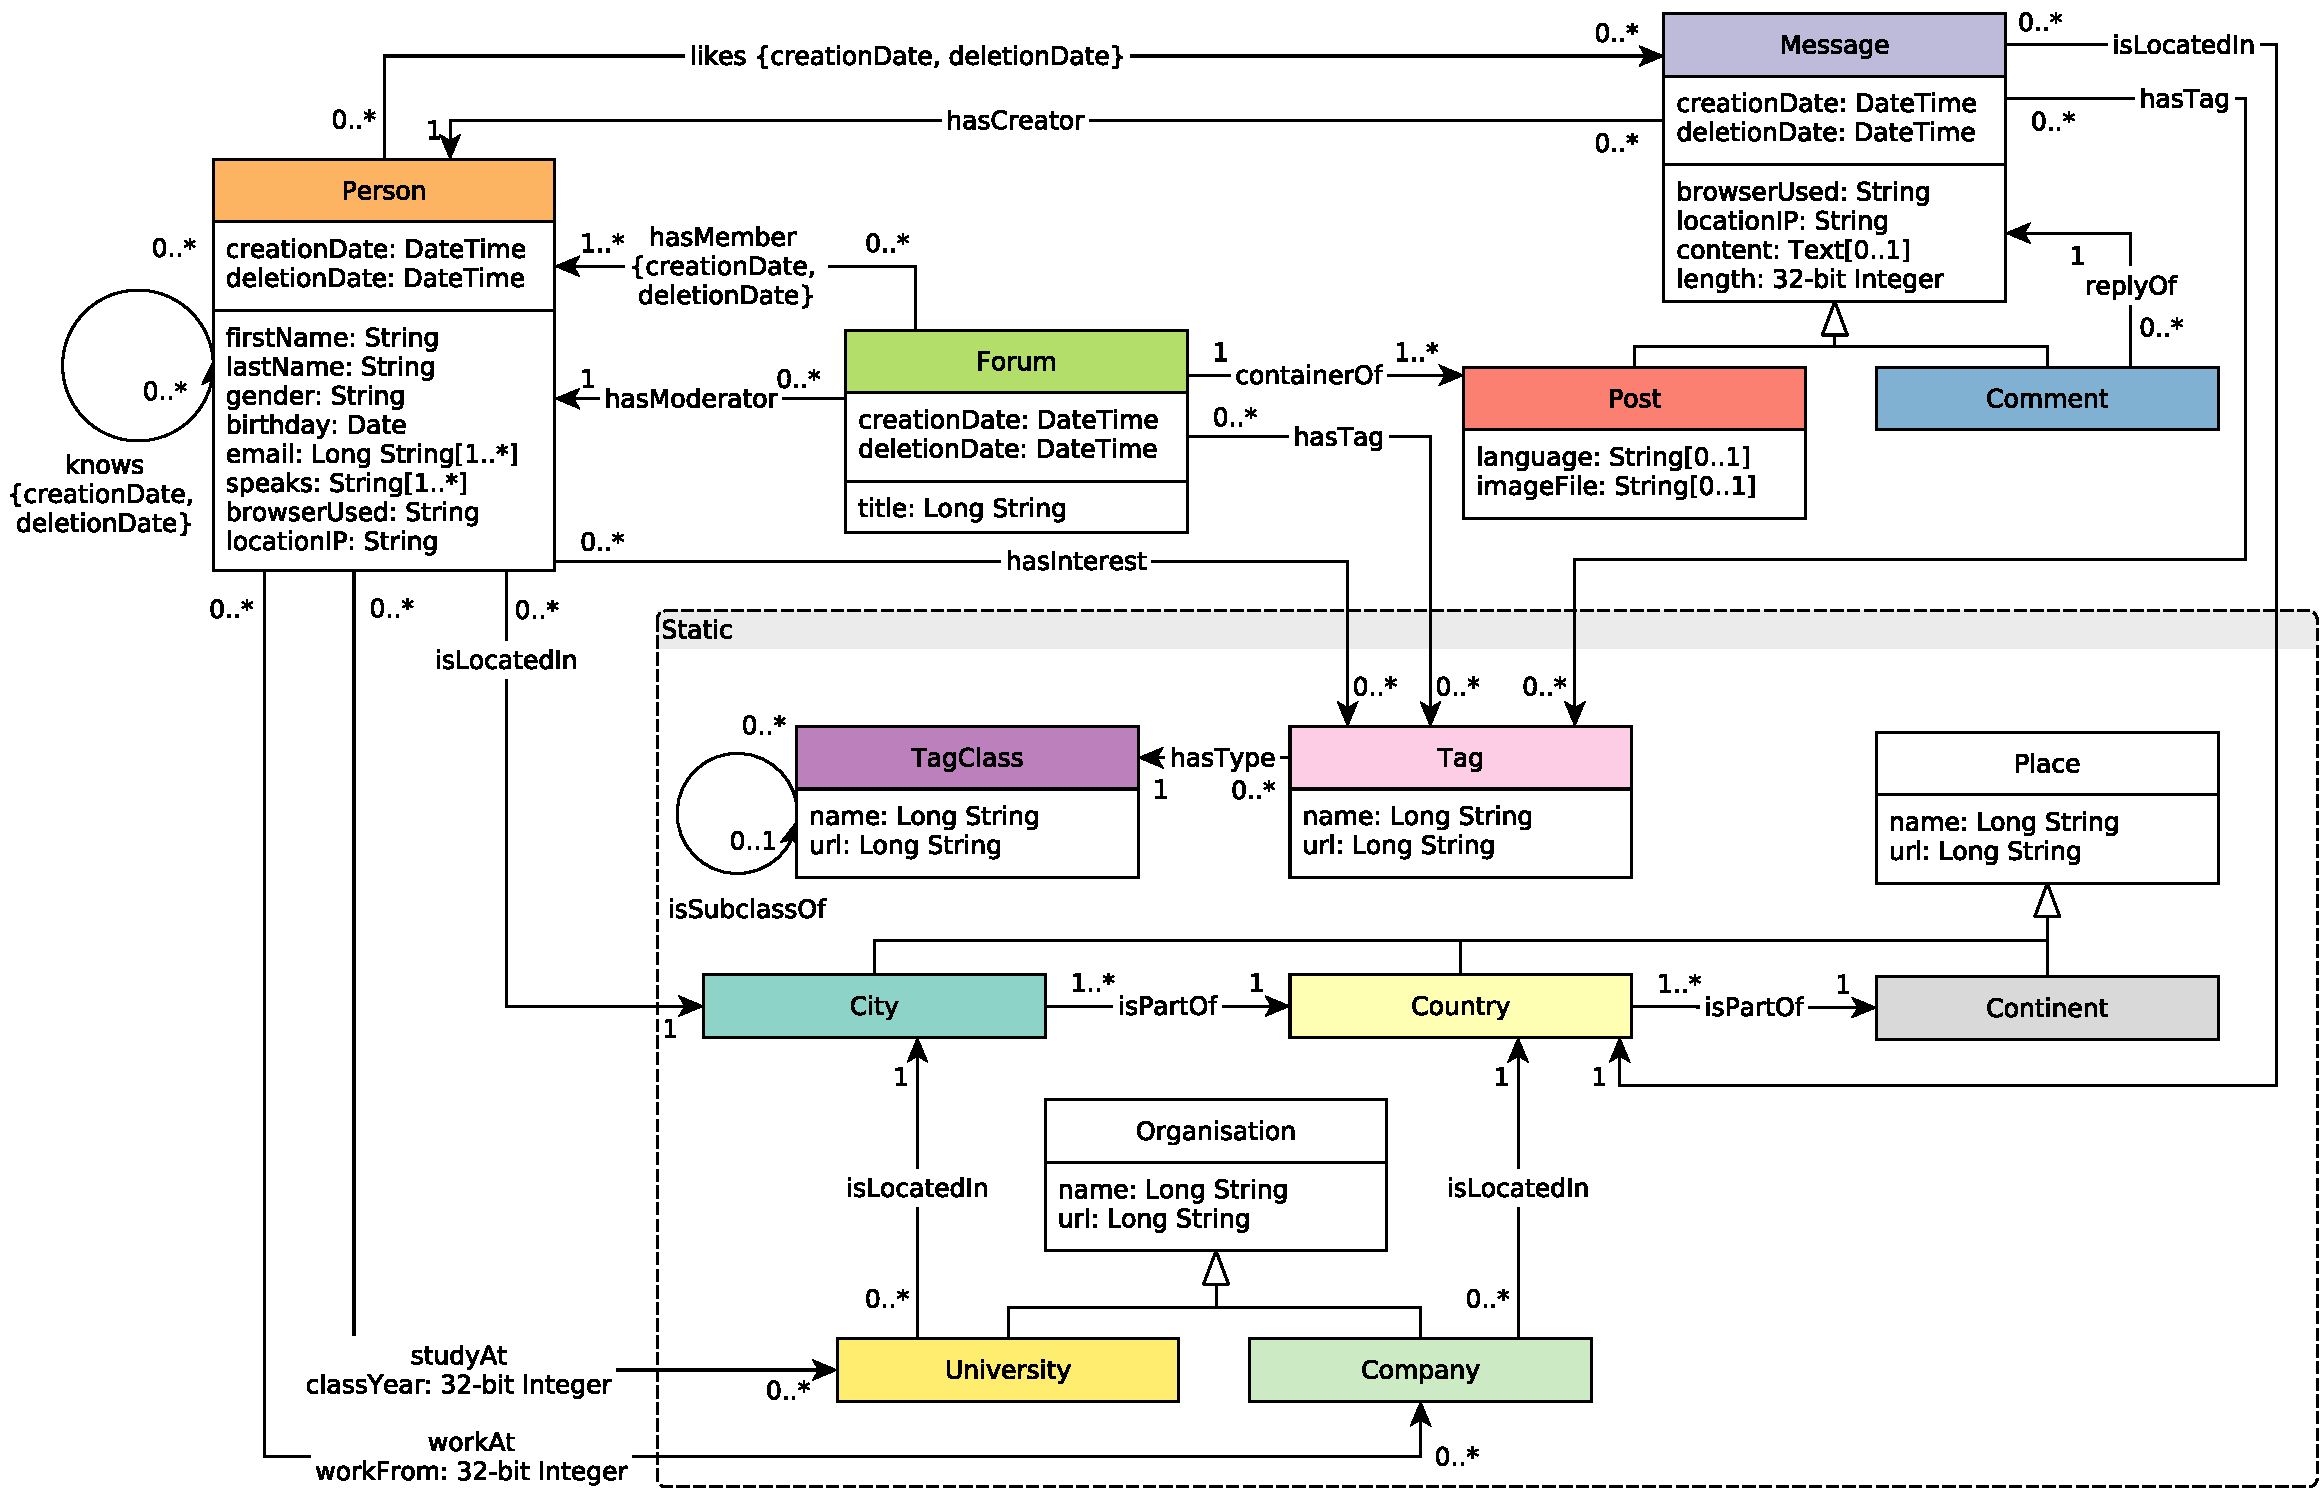
\includegraphics[width=\linewidth]{figures/schema}
	\caption{The \ldbcsnb data schema}
	\label{figure:schema}
\end{figure}

The schema specifies different entities, their attributes and their relations.
All of them are described in the following sections.

{\flushleft \textbf{Textual Restrictions and Notes}}
\begin{itemize}
    \item Posts have content or imageFile. They have one of them but not both. The one they do not have is an empty string.
    \item Posts in a forum can be created by a non-member person if and only if that person is a modeartor.
\end{itemize}

\subsubsection{Entities}

{\flushleft \textbf{City:}} a sub-class of a Place, and represents a
city of the real world. City entities are used to specify where persons live,
as well as where universities operate.

{\flushleft \textbf{Comment:}} a sub-class of a Message, and represents a
comment made by a person to an existing message (either a Post or a Comment).

{\flushleft \textbf{Company:}} a sub-class of an Organisation, and represents a company where persons work.


{\flushleft \textbf{Country:}} a sub-class of a Place, and represents a continent of the real world.


{\flushleft \textbf{Forum:}} a meeting point where people
post messages. Forums are characterized by the topics (represented as tags)
people in the forum are talking about. Although from the schema's perspective
it is not evident, there exist three different types of
forums: persons' personal walls, image albums, and groups. They are
distinguished by their titles. \autoref{table:forum} shows the attributes
of Forum entity.

\begin{table}[H]
    \begin{tabular}{|>{\varNameCell}p{\attributeColumnWidth}|>{\typeCell}p{\typeColumnWidth}|p{\descriptionColumnWidth}|}
        \hline
        \tableHeaderFirst{Attribute} & \tableHeader{Type} & \tableHeader{Description} \\
        \hline
        id & ID  & The identifier of the forum.\\
        \hline
        title & Long String  & The title of the forum.\\
        \hline
        creationDate & DateTime  & The date the forum was created.\\
        \hline
    \end{tabular}
    \caption{Attributes of Forum entity.}
    \label{table:forum}
\end{table}

{\flushleft \textbf{Message:}} an abstract entity that represents a message
created by a person. \autoref{table:message} shows the attributes of Message
abstract entity.

\begin{table}[H]
    \begin{tabular}{|>{\varNameCell}p{\attributeColumnWidth}|>{\typeCell}p{\typeColumnWidth}|p{\descriptionColumnWidth}|}
        \hline
        \tableHeaderFirst{Attribute} & \tableHeader{Type} & \tableHeader{Description} \\
        \hline
        id & ID  & The identifier of the message.\\
        \hline
        browserUsed & String  & The browser used by the Person to create the message.\\
        \hline
        creationDate & DateTime  & The date the message was created.\\
        \hline
        locationIP & String  & The IP of the location from which the message was created.\\
        \hline
        content & Text[0..1]  & The content of the message.\\
        \hline
        length & 32-bit Integer  & The length of the content.\\
        \hline
    \end{tabular}
    \caption{Attributes of Message interface.}
    \label{table:message}
\end{table}

{\flushleft \textbf{Organisation:}} an institution of the real
world. \autoref{table:organisation} shows the attributes of Organisation
entity.

\begin{table}[H]
    \begin{tabular}{|>{\varNameCell}p{\attributeColumnWidth}|>{\typeCell}p{\typeColumnWidth}|p{\descriptionColumnWidth}|}
        \hline
        \tableHeaderFirst{Attribute} & \tableHeader{Type} & \tableHeader{Description} \\
        \hline
        id & ID  & The identifier of the organisation.\\
        \hline
        name & Long String  & The name of the organisation.\\
        \hline
        url & Long String  & The URL of the organisation.\\
        \hline
    \end{tabular}
    \caption{Attributes of Organisation entity.}
    \label{table:organisation}
\end{table}

{\flushleft \textbf{Person:}} the avatar a real world person creates
when he/she joins the network, and contains various information about the
person as well as network related information. \autoref{table:person} shows
the attributes of Person entity.

\begin{table}[H]
    \begin{tabular}{|>{\varNameCell}p{\attributeColumnWidth}|>{\typeCell}p{\typeColumnWidth}|p{\descriptionColumnWidth}|}
        \hline
        \tableHeaderFirst{Attribute} & \tableHeader{Type} & \tableHeader{Description} \\
        \hline
        id & ID  & The identifier of the person.\\
        \hline
        firstName & String  & The first name of the person.\\
        \hline
        lastName & String  & The last name of the person.\\
        \hline
        gender & String  & The gender of the person.\\
        \hline
        birthday & Date  & The birthday of the person.\\
        \hline
        email & Long String[1..*]  & The set of emails the person has.\\
        \hline
        speaks & String[1..*]  & The set of languages the person speaks.\\
        \hline
        browserUsed & String  & The browser used by the person when he/she registered to the social network.\\
        \hline
        locationIP & String  & The IP of the location from which the person was registered to the social network.\\
        \hline
        creationDate & DateTime  & The date the person joined the social network.\\
        \hline
    \end{tabular}
    \caption{Attributes of Person entity.}
    \label{table:person}
\end{table}


{\flushleft \textbf{Place:}} a place in the world.
\autoref{table:place} shows the attributes of Place entity.

\begin{table}[H]
    \begin{tabular}{|>{\varNameCell}p{\attributeColumnWidth}|>{\typeCell}p{\typeColumnWidth}|p{\descriptionColumnWidth}|}
        \hline
        \tableHeaderFirst{Attribute} & \tableHeader{Type} & \tableHeader{Description} \\
        \hline
        id & ID  & The identifier of the place.\\
        \hline
        name & Long String  & The name of the place.\\
        \hline
        url & Long String  & The URL of the place.\\
        \hline
    \end{tabular}
    \caption{Attributes of Place entity.}
    \label{table:place}
\end{table}

{\flushleft \textbf{Post:}} a sub-class of Message, that is posted in a
forum. Posts are created by persons into the forums where they belong.
Posts contain either content or imageFile, always one of them but never both.
The one they do not have is an empty string.
\autoref{table:post} shows the attributes of Post entity.

\begin{table}[H]
    \begin{tabular}{|>{\varNameCell}p{\attributeColumnWidth}|>{\typeCell}p{\typeColumnWidth}|p{\descriptionColumnWidth}|}
        \hline
        \tableHeaderFirst{Attribute} & \tableHeader{Type} & \tableHeader{Description} \\
        \hline
        language & String[0..1]  & The language of the post.\\
        \hline
        imageFile & String[0..1]  & The image file of the post.\\
        \hline
    \end{tabular}
    \caption{Attributes of Post entity.}
    \label{table:post}
\end{table}

{\flushleft \textbf{Tag:}} a topic or a concept. Tags are used to
specify the topics of forums and posts, as well as the topics a person is
interested in. \autoref{table:tag} shows the attributes of Tag entity.

\begin{table}[H]
    \begin{tabular}{|>{\varNameCell}p{\attributeColumnWidth}|>{\typeCell}p{\typeColumnWidth}|p{\descriptionColumnWidth}|}
        \hline
        \tableHeaderFirst{Attribute} & \tableHeader{Type} & \tableHeader{Description} \\
        \hline
        id & ID  & The identifier of the tag.\\
        \hline
        name & Long String  &  The name of the tag.\\
        \hline
        url & Long String  &  The URL of the tag.\\
        \hline
    \end{tabular}
    \caption{Attributes of Tag entity.}
    \label{table:tag}
\end{table}

{\flushleft \textbf{TagClass:}} a class or a category used to build
a hierarchy of tags. \autoref{table:tagclass} shows the attributes of TagClass
entity.

\begin{table}[H]
    \begin{tabular}{|>{\varNameCell}p{\attributeColumnWidth}|>{\typeCell}p{\typeColumnWidth}|p{\descriptionColumnWidth}|}
        \hline
        \tableHeaderFirst{Attribute} & \tableHeader{Type} & \tableHeader{Description} \\
        \hline
        id & ID  & The identifier of the tagclass.\\
        \hline
        name & Long String  &  The name of the tagclass.\\
        \hline
        url & Long String  &  The URL of the tagclass.\\
        \hline
    \end{tabular}
    \caption{Attributes of TagClass entity.}
    \label{table:tagclass}
\end{table}

{\flushleft \textbf{University:}} a sub-class of Organisation,
and represents an institution where persons study.

\subsubsection{Relations}

Relations connect entities of different types. Entities are defined by their ''id'' attribute.

\begin{longtable}{|>{\varNameCell}p{2.5cm}|>{\typeCell}p{2.5cm}|>{\typeCell}p{2.5cm}|>{\edgeDirectionCell}c|p{6.5cm}|}
       \hline
        \tableHeaderFirst{Name} & \tableHeader{Tail} & \tableHeader{Head} & \tableHeader{Type} & \tableHeader{Description} \\
        \hline
        containerOf & Forum[1] & Post[1..*] & D & A Forum and a Post contained in it\\
        \hline
        hasCreator & Message[0..*] & Person[1] & D & A Message and its creator (Person)\\
        \hline
        hasInterest & Person[0..*] & Tag[0..*] & D & A Person and a Tag representing a topic the person is interested in\\
        \hline
        hasMember & Forum[0..*] &  Person[1..*] & D & A  Forum and a member (Person) of the forum

        \attributeTable{joinDate}{DateTime}{The Date the person joined the forum}

        \\
        \hline
        hasModerator & Forum[0..*] & Person[1] & D & A Forum and its moderator (Person) \\
        \hline
        hasTag & Message[0..*] & Tag[0..*] & D & A Message and a Tag representing the message's topic \\
        \hline
        hasTag & Forum[0..*] & Tag[0..*] & D & A Forum and a Tag representing the forum's topic \\
        \hline
        hasType & Tag[0..*] & TagClass[1] & D & A Tag and a TagClass the tag belongs to \\
        \hline
        isLocatedIn & Company[0..*] & Country[1] & D & A Company and its home Country \\
        \hline
        isLocatedIn & Message[0..*] & Country[1] & D & A Message and the Country from which it was issued \\
        \hline
        isLocatedIn & Person[0..*] & City[1] & D & A Person and their home City \\
        \hline
        isLocatedIn & University[0..*] & City[1] & D &  A University and the City where the university is \\
        \hline
        isPartOf & City[1..*] & Country[1] & D & A City and the Country it is part of \\
        \hline
        isPartOf & Country[1..*] & Continent[1] & D & A Country and the Continent it is part of \\
        \hline
        isSubclassOf & TagClass[0..*] & TagClass[0..1] & D & A TagClass and its parent TagClass \\
        \hline
        knows & Person[0..*] & Person[0..*] & U & Two Persons that know each other

        \attributeTable{creationDate}{DateTime}{The date the knows relation was established}

        \\
        \hline
        likes & Person[0..*] & Message[0..*] & D & A Person that likes a Message

		\attributeTable{creationDate}{DateTime}{The date the like was issued}

        \\
        \hline
        replyOf & Comment[0..*] & Message[1] & D & A Comment and the Message it replies \\
        \hline
        studyAt & Person[0..*] & University[0..*] & D & A Person and a University it has studied

		\attributeTable{classYear}{32-bit Integer}{The year the person graduated}

        \\
        \hline
        workAt & Person[0..*] & Company[0..*] & D & A Person and a Company it works

		\attributeTable{workFrom}{32-bit Integer}{The year the person started to work at that company}

        \\
        \hline
        \caption{Description of the data relations.}
        \label{table:relations}
\end{longtable}

\subsubsection{Domain Concepts}

A \emph{thread} consists of Messages, starting with a single Post and Comments that transitively reply to that Post.

\subsection{Data Generation}
\label{section:data_generation}

\ldbcsnb provides \datagen (Data Base Generator), which produces synthetic
datasets following the schema described above. Data
produced mimics a social network's activity during a period of time. Three
parameters determine the generated data: the number of persons, the number of
years simulated, and the starting year of simulation. \datagen is defined by the
following characteristics:

\begin{itemize}
    \item \textbf{Realism.} Data generated by \datagen mimics the
        characteristics of those found in a real social network. In \datagen,
        output attributes, cardinalities, correlations and distributions have
        been finely tuned to reproduce a real social network in each of its
        aspects On the one hand, it is aware of the  data and link distributions
        found in a real social network such as Facebook. On the other hand, it
        uses real data from DBpedia, such as property dictionaries, which are
        used to ensure that attribute values are realistic and correlated.
    \item \textbf{Scalability.} Since \ldbcsnb targets systems of different
        scales and budgets, \datagen is capable of generating datasets of
        different sizes, from a few Gigabytes to Terabytes. \datagen is
        implemented following the MapReduce parallel paradigm, allowing the
        generation of small datasets in single node machines, as well as large
        datasets on commodity clusters.
    \item \textbf{Determinism.} \datagen is deterministic regardless of the number
        of cores/machines used to produce the data. This important feature
        guarantees that all Test Sponsors will face the same dataset,
        thus, making the comparisons between different systems fair and the
        benchmarks' results reproducible.
    \item \textbf{Usability.} \ldbcsnb is designed to have an affordable entry
        point. As such, \datagen's design is  severely influenced by this
        philosophy, and therefore it is designed to be as easy to use as
        possible.
\end{itemize}


\subsubsection{Resource Files}

\datagen uses a set of resource files with data
extracted from DBpedia. Conceptually, \datagen generates attribute's
values following a property dictionary model that is defined by

\begin{itemize}
    \item a dictionary $D$
    \item a ranking function $R$
    \item a probability function $F$
\end{itemize}

Dictionary D is a fixed set of values. The ranking function R is a bijection
that assigns to each value in a dictionary a unique rank between 1 and |$D$|.
The probability density function $F$ specifies how the data generator chooses
values from dictionary $D$ using the rank for each term in the dictionary. The
idea to have a separate ranking and probability function is motivated by the
need of generating correlated values: in particular, the ranking function is
typically parameterized by some parameters: different parameter values result
in different rankings. For example, in the case of a dictionary of property
firstName, the popularity of first names, might depend on the gender, country
and birthday properties. Thus, the fact that the popularity of first names in
different countries and times is different, is reflected by the different ranks
produced by function $R$ over the full dictionary of names.  \datagen uses a
dictionary for each literal property, as well as ranking functions for all
literal properties. These are materialized in a set of resource files, which
are described in \autoref{table:property_dictionaries}.

\begin{table}[H]
\begin{tabular}{|p{4cm}|p{12cm}|}
    \hline
    \tableHeaderFirst{Resource Name} & \tableHeader{Description} \\
    \hline
    Browsers & Contains a list of web browsers and their probability to be used. It is used to set the browsers used by the users.\\
    \hline
    Cities by Country & Contains a list of cites and the country they belong. It is used to assign cities to users and universities.\\
    \hline
    Companies by Country & Contains the set of companies per country. It is used to set the countries where companies operate.\\
    \hline
    Countries & Contains a list of countries and their populations. It is used to obtain the amount of people generated for each country.\\
    \hline
    Emails & Contains the set of email providers. It is used to generate the email accounts of persons.\\
    \hline
    IP Zones & Contains the set of IP ranges assigned to each country. It is used to assign the IP addresses to users.\\
    \hline
    Languages by Country & Contains the set of languages spoken in each country. It is used to set the languages spoken by each user.\\
    \hline
    Name by Country & Contains the set of names and the probability to appear in each country. It is used to assign names to persons, correlated with their countries.\\
    \hline
    Popular places by Country & Contains the set of popular places per country. These are used to set where images attached to posts are taken from.\\
    \hline
    Surnames' by Country & Contains the set of surnames and the probability to appear in each country. It is used to assign surnames to persons, correlated with their countries.\\
    \hline
    Tags by Country & Contains a set of tags and their probability to appear in each country. It is used to assign the interests to persons and forums.\\
    \hline
    Tag Classes & Contains, for each tag, the classes it belongs to.\\
    \hline
    Tag Hierarchies & Contains, for each tagClass, their parent tagClass.\\
    \hline
    Tag Matrix & Contains, for each tag, the correlation probability with the other tags. It is used enrich the tags associated to messages.\\
    \hline
    Tag Text & Contains, for each tag, a text. This is used to generate the text for messages.\\
    \hline
    Universities by City & Contains the set of universities per city. It is used to set the cities where universities operate.\\
    \hline
\end{tabular}
    \caption{Resource files}
    \label{table:property_dictionaries}
\end{table}

\subsubsection{Graph Generation}

\autoref{figure:generation_process} conceptually depicts the full data
generation process. The first step loads all the dictionaries and resource
files, and initializes the \datagen parameters.  Second, it generates all the
Persons in the graph, and the minimum necessary information to operate. Part of
these information are the interests of the persons, and the number of knows
relationships of every person, which is guided by a degree distribution
function similar to that found in Facebook~\cite{facebook_anatomy}.

The next three steps are devoted to the creation of knows relationships.  An
important aspect of real social networks, is the fact that similar persons
(with similar interests and behaviors) tend to be connected. This is known as
the Homophily principle~\cite{mcpherson2001birds,DBLP:journals/socnet/BaroneC18}, and implies the presence of
a larger amount of triangles than that expected in a random network. In order
to reproduce this characteristic, \datagen generates the edges by means of
correlation dimensions.  Given a person, the probability to be connected to
another person is typically skewed with respect to some similarity between the
persons. That is, for a person $n$ and for a small set of persons that are
somehow similar to it, there is a high connectivity probability, whereas for
most other persons, this probability is quite low. This knowledge is
exploited by \datagen to reproduce correlations.

\begin{figure}[H]
    \centering
    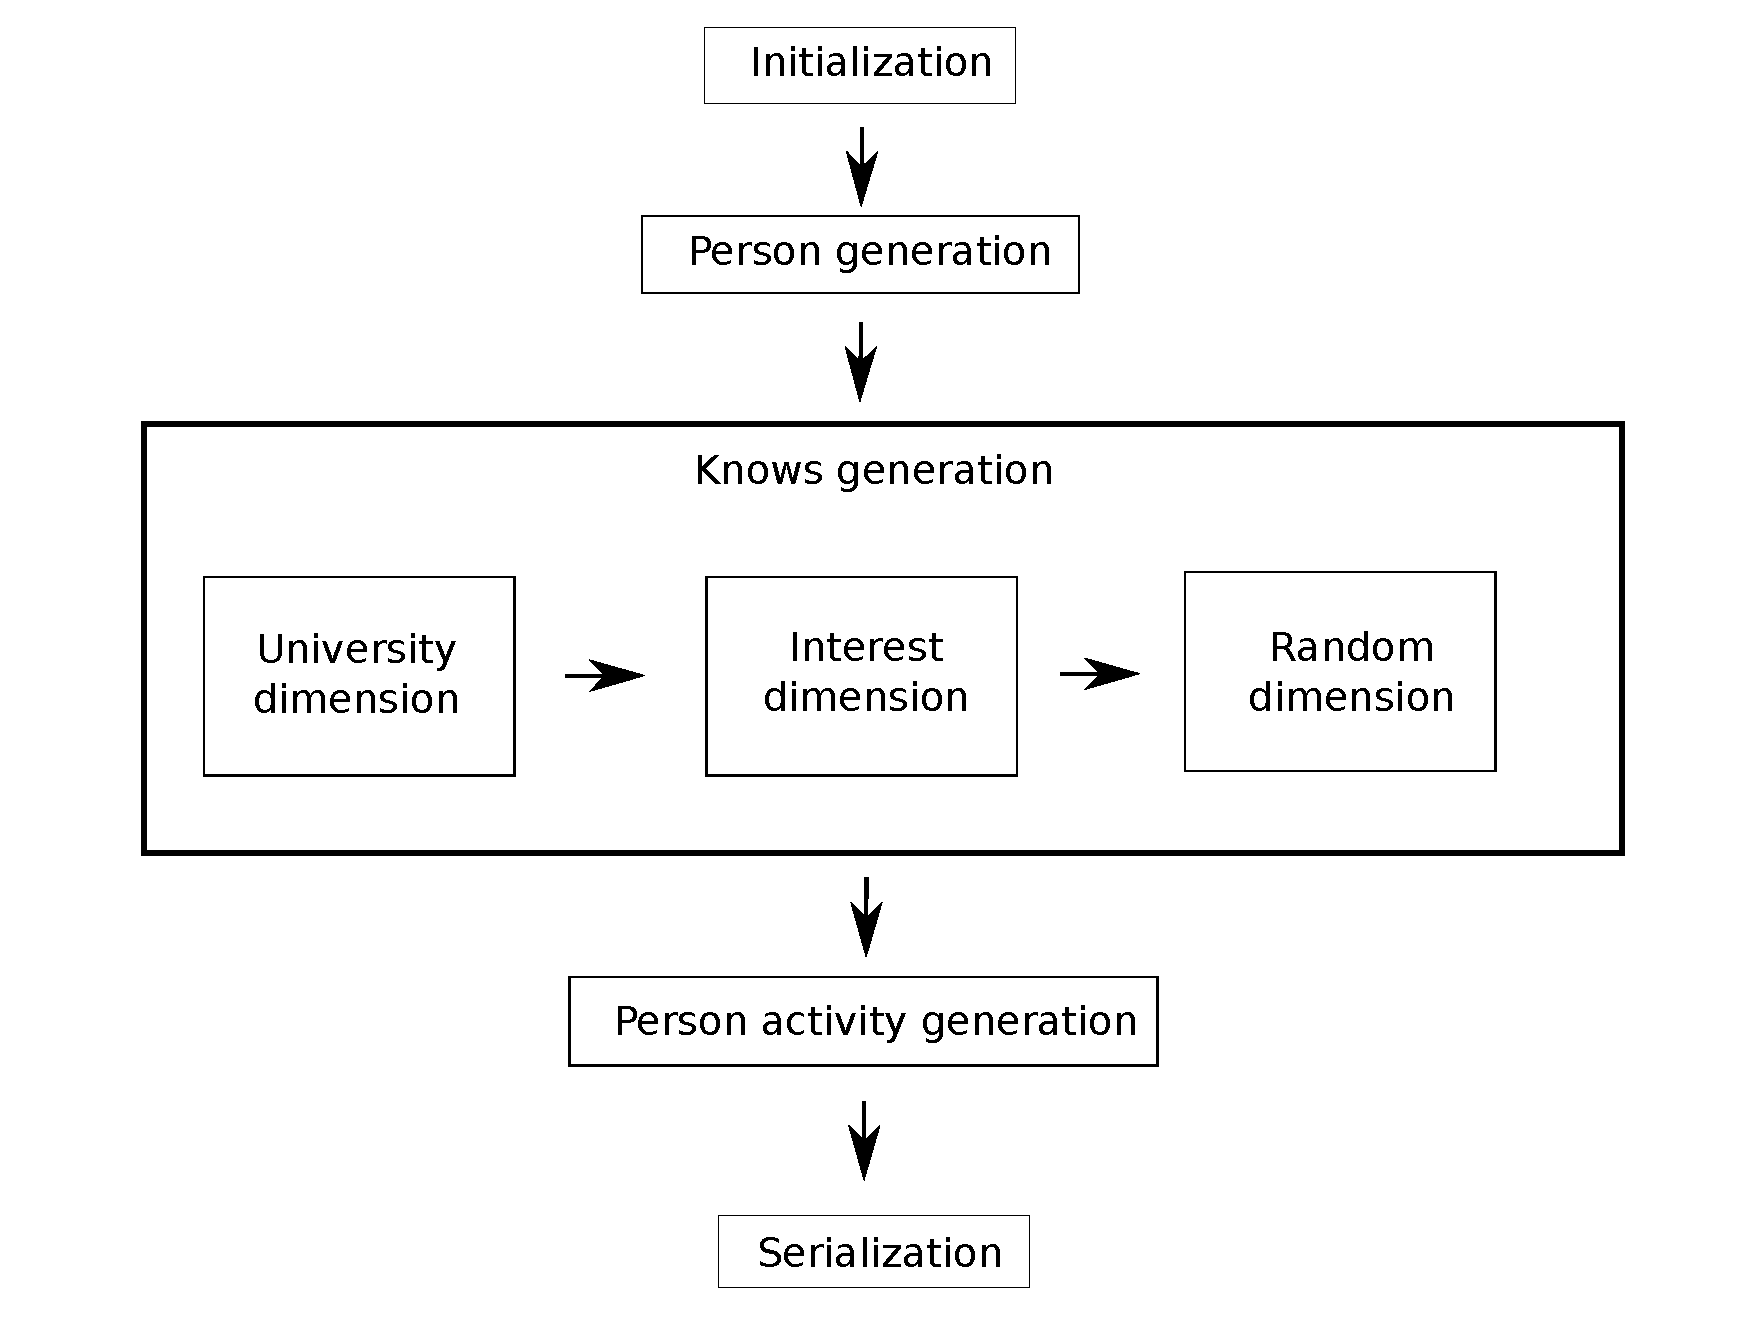
\includegraphics[width=1\linewidth]{figures/sndg/execution.pdf}
    \caption{The \datagen generation process.}
    \label{figure:generation_process}
\end{figure}

Given a similarity function $M(x) : n \rightarrow [0, \infty]$ that gives a score to a person,
with the characteristic that two similar persons will have similar scores, we
can sort all the persons by function $M$ and compare a person $n$ against only the
$W$ neighboring persons in the sorted array. The consequence of this approach is
that similar persons are grouped together, and the larger the
distance between two persons indicates a monotonic increase in their similarity
difference. In order to choose the persons to connect, \datagen uses a geometric
probability distribution that provides a probability for picking persons to
connect, that are between 1 and $W$ positions apart in the similarity
ranking.

Similarity functions and probability distribution functions over ranked
distance drive what kind of persons will be connected with an edge, not how
many. As stated above, the number of friends of a person is determined by a
Facebook-like distribution. The edges that will be connected to a person $n$,
are selected by randomly picking the required number of edges according to the
correlated probability distributions as discussed before. In the case that
multiple correlations exist, another probability function is used to divide the
intended number of edges between the various correlation dimensions. In \datagen,
three correlated dimensions are chosen: the first one depends on where the
person studied and when, and the second correlation dimension depends on the
interests of the person, and the third one is random (to reproduce the random
noise present in real data). Thus, \datagen has a Facebook-like distributed node
degree, and a predictable (but not fixed) average split between the reasons for
creating edges.

In the next step, person's activity, in the form of forums, posts and comments
is created. \datagen reproduces the fact that people with a larger number of
friends have a higher activity, and hence post more photos and comments to a
larger number of posts. Another important characteristic of real users'
activity in social network, are time correlations.  Usually, users' posts
creation in a social network is driven by real world events.  For
instance, one may think about an important event such as the elections in a
country, or a natural disaster. Around the time these events occur, network
activity about these events' topics sees an increase in volume. \datagen
reproduces these characteristics with the simulation of what we name as
flashmob events.  Several events are generated randomly at the beginning of the
generation process, which are assigned a random tag, and are given a time and
an intensity which represents the repercussion of the event in the real world.
When persons' posts are created, some of them are classified as flashmob posts,
and their topics and dates are assigned based on the generated flashmob events.
The volume of activity around this events is modeled following a model similar
to that described in~\cite{DBLP:conf/kdd/LeskovecBKT08}. Furthermore, in order to reproduce the
more uniform every day's user activity, \datagen also generates post uniformly
distributed along all the simulated time.

Finally, in the last step the data is serialized into the output files.

\subsubsection{Implementation Details}

\datagen is implemented using the MapReduce parallel paradigm. In MapReduce, a
Map function runs on different parts of the input data, in parallel and on many
node clusters. This function processes the input data and produces for each
result a key. Reduce functions then obtain this data and Reducers run in
parallel on many cluster nodes. The produced key simply determines the Reducer
to which the results are sent. The use of the MapReduce paradigm allows the
generator to scale considerably, allowing the generation of huge datasets by
using clusters of machines.

In the case of \datagen, the overall process is divided into three MapReduce jobs.
In the first job, each mapper generates a subset of the persons of the graph. A
key is assigned to each person using one of the similarity functions described
above. Then, reducers receive the the key-value pairs sorted by the key,
generate the knows relations following the described windowing process, and
assign to each person a new key based on another similarity function, for the
next MapReduce pass.  This process can be successively repeated for additional
correlation dimension.  Finally, the last reducer generates the remaining
information such as forums, posts and comments.


\subsection{Output Data}

\datagen produces outputs three different items:
\begin{itemize}
  \item \textbf{Dataset}: The dataset to be bulk loaded by the SUT. It
    corresponds to roughly the 90\% of the total generated network.
  \item \textbf{Update Streams}: A set of update streams containing update
    queries, which are used by the driver to generate the update queries of the
    workloads. This update
    streams correspond to the remaining 10\% of the generated dataset.
  \item \textbf{Substitution Parameters}: A set of files containing the
    different parameter bindings that will be used by the driver to generate the
    read queries of the workloads.
\end{itemize}

The SUT have to take care only of the generated Dataset to be bulk loaded.
The formats currently supported by \datagen are the following:

\begin{itemize}
  \item \textbf{CSV variants:}
    \begin{itemize}
      \item \textbf{CSVBasic:} Data output in CSV format, one file per different entity and on file
        per different relation. Also, there is a file for those attributes whose
        cardinality is larger than one (\ie Person.email, Person.speaks).
      \item \textbf{CSVMergeForeign:} Similar to the CSV format, but in this case, those
        relations of the form 1 to 1 and 1 to N, are stored in the tail entity file as
        a foreign keys.
      \item \textbf{CSVComposite:} Similar to the CSV format, but uses composite attributes for storing the Person.email, Person.speaks attributes.
      \item \textbf{CSVCompositeMergeForeign:} Has the traits of both the CSVComposite and the CSVMergeForeign formats.
    \end{itemize}
  \item \textbf{Turtle:} Dataset in Turtle format for RDF systems.
\end{itemize}



\subsubsection{CSV}

This is a comma separated format. Each entity, relation and properties with a
cardinality larger than one, are output in a separate file. Generated files are
summarized at \autoref{table:csv}.  Depending on the number of threads used
for generating the dataset, the number of files varies, since there is a file
generated per thread. The * in the file names indicates a number between 0 and
$\mathsf{NumberOfThreads}-1$.

\begin{table}[htb]
    \scriptsize
    \centering
    \begin{tabular}{|p{4.6cm}|p{9.8cm}|}
    	\hline
    	\tableHeaderFirst{File}                 & \tableHeader{Content}                                                                   \\ \hline
    	comment\_*.csv                          & id | creationDate | locationIP | browserUsed | content | length                         \\ \hline
    	comment\_hasCreator\_person\_*.csv      & Comment.id | Person.id                                                                  \\ \hline
    	comment\_hasTag\_tag\_*.csv             & Comment.id | Tag.id                                                                     \\ \hline
    	comment\_isLocatedIn\_place\_*.csv      & Comment.id | Place.id                                                                   \\ \hline
    	comment\_replyOf\_comment\_*.csv        & Comment.id | Comment.id                                                                 \\ \hline
    	comment\_replyOf\_post\_*.csv           & Comment.id | Post.id                                                                    \\ \hline
    	forum\_*.csv                            & id | title | creationDate                                                               \\ \hline
    	forum\_containerOf\_post\_*.csv         & Forum.id | Post.id                                                                      \\ \hline
    	forum\_hasMember\_person\_*.csv         & Forum.id | Person.id | joinDate                                                         \\ \hline
    	forum\_hasModerator\_person\_*.csv      & Forum.id | Person.id                                                                    \\ \hline
    	forum\_hasTag\_tag\_*.csv               & Forum.id | Tag.id                                                                       \\ \hline
    	organisation\_*.csv                     & id | type({"university", "company"}) | name | url                                       \\ \hline
    	organisation\_isLocatedIn\_place\_*.csv & Organisation.id | Place.id                                                              \\ \hline
    	person\_*.csv                           & id | firstName | lastName | gender | birthday | creationDate | locationIP | browserUsed \\ \hline
    	person\_email\_emailaddress\_*.csv      & Person.id | email                                                                       \\ \hline
    	person\_hasInterest\_tag\_*.csv         & Person.id | Tag.id                                                                      \\ \hline
    	person\_isLocatedIn\_place\_*.csv       & Person.id | Place.id                                                                    \\ \hline
    	person\_knows\_person\_*.csv            & Person.id | Person.id | creationDate                                                    \\ \hline
    	person\_likes\_comment\_*.csv           & Person.id | Post.id | creationDate                                                      \\ \hline
    	person\_likes\_post\_*.csv              & Person.id | Post.id | creationDate                                                      \\ \hline
    	person\_speaks\_language\_*.csv         & Person.id | language                                                                    \\ \hline
    	person\_studyAt\_organisation\_*.csv    & Person.id | Organisation.id | classYear                                                 \\ \hline
    	person\_workAt\_organisation\_*.csv     & Person.id | Organisation.id | workFrom                                                  \\ \hline
    	place\_*.csv                            & id | name | url | type({"city", "country", "continent"})                                \\ \hline
    	place\_isPartOf\_place\_*.csv           & Place.id | Place.id                                                                     \\ \hline
    	post\_*.csv                             & id | imageFile | creationDate | locationIP | browserUsed | language | content | length  \\ \hline
    	post\_hasCreator\_person\_*.csv         & Post.id | Person.id                                                                     \\ \hline
    	post\_hasTag\_tag\_*.csv                & Post.id | Tag.id                                                                        \\ \hline
    	post\_isLocatedIn\_place.csv            & Post.id | Place.id                                                                      \\ \hline
    	tag\_*.csv                              & id | name | url                                                                         \\ \hline
    	tag\_hasType\_tagclass\_*.csv           & Tag.id | TagClass.id                                                                    \\ \hline
    	tagclass\_*.csv                         & id | name | url                                                                         \\ \hline
    	tagclass\_isSubclassOf\_tagclass\_*.csv & TagClass.id | TagClass.id                                                               \\ \hline
    \end{tabular}
    \caption{Files output by the CSV serializer (33 in total)}
    \label{table:csv}
\end{table}



\subsubsection{CSV\_MERGE\_FOREIGN}

This is a comma separated format. It is similar to CSV, but those relations
connecting two entities A and B, where an entity A has a cardinality of one, A
is output as a column of entity B. Generated files are summarized at
\autoref{table:csv_merge_foreign}. Depending on the number of threads used for generating
the dataset, the number of files varies, since there is a file generated per
thread. The * in the file names indicates a number between 0 and $\mathsf{NumberOfThreads}-1$.

\begin{table}[htb]
    \scriptsize
    \centerline{\begin{tabular}{|p{4.3cm}|p{12.4cm}|}
        \hline
		\tableHeaderFirst{File}              & \tableHeader{Content}                                                                                               \\ \hline\hline
		organisation\_*.csv                  & id | type({"university", "company"}) | name | url | place                                                           \\ \hline
		place\_*.csv                         & id | name | url | type({"city", "country", "continent"}) | isPartOf                                                 \\ \hline
		tag\_*.csv                           & id | name | url | hasType                                                                                           \\ \hline
		tagclass\_*.csv                      & id | name | url | isSubclassOf                                                                                      \\ \hline\hline
        comment\_*.csv                       & id | creationDate | locationIP | browserUsed | content | length | creator | place | replyOfPost | replyOfComment    \\ \hline
        comment\_hasTag\_tag\_*.csv          & Comment.id | Tag.id                                                                                                 \\ \hline
        forum\_*.csv                         & id | title | creationDate | moderator                                                                               \\ \hline
        forum\_hasMember\_person\_*.csv      & Forum.id | Person.id | joinDate                                                                                     \\ \hline
        forum\_hasTag\_tag\_*.csv            & Forum.id | Tag.id                                                                                                   \\ \hline
		person\_*.csv                        & id | firstName | lastName | gender | birthday | creationDate | locationIP | browserUsed | place                     \\ \hline
        person\_email\_emailaddress\_*.csv   & Person.id | email                                                                                                   \\ \hline
        person\_hasInterest\_tag\_*.csv      & Person.id | Tag.id                                                                                                  \\ \hline
        person\_knows\_person\_*.csv         & Person.id | Person.id | creationDate                                                                                \\ \hline
        person\_likes\_comment\_*.csv        & Person.id | Post.id | creationDate                                                                                  \\ \hline
        person\_likes\_post\_*.csv           & Person.id | Post.id | creationDate                                                                                  \\ \hline
        person\_speaks\_language\_*.csv      & Person.id | language                                                                                                \\ \hline
        person\_studyAt\_organisation\_*.csv & Person.id | Organisation.id | classYear                                                                             \\ \hline
        person\_workAt\_organisation\_*.csv  & Person.id | Organisation.id | workFrom                                                                              \\ \hline
        post\_*.csv                          & id | imageFile | creationDate | locationIP | browserUsed | language | content | length | creator | Forum.id | place \\ \hline
        post\_hasTag\_tag\_*.csv             & Post.id | Tag.id                                                                                                    \\ \hline
    \end{tabular}}
    \caption{Files output by the CsvMergeForeign serializer (20 in total)}
    \label{table:csv_merge_foreign}
\end{table}


\begin{table}[htb]
    \scriptsize
    \centering
    \begin{tabular}{|c|p{4.6cm}|p{11.4cm}|}
    	\hline
    	\tableHeaderFirst{Ent.} & \tableHeader{File}                      & \tableHeader{Content}                                                                                       \\ \hline\hline
        N                       & organisation\_*.csv                     & id | type({"university", "company"}) | name | url                                                           \\ \hline
        E                       & organisation\_isLocatedIn\_place\_*.csv & Organisation.id | Place.id                                                                                  \\ \hline
        N                       & place\_*.csv                            & id | name | url | type({"city", "country", "continent"})                                                    \\ \hline
        E                       & place\_isPartOf\_place\_*.csv           & Place.id | Place.id                                                                                         \\ \hline
        N                       & tag\_*.csv                              & id | name | url                                                                                             \\ \hline
        E                       & tag\_hasType\_tagclass\_*.csv           & Tag.id | TagClass.id                                                                                        \\ \hline
        N                       & tagclass\_*.csv                         & id | name | url                                                                                             \\ \hline
        E                       & tagclass\_isSubclassOf\_tagclass\_*.csv & TagClass.id | TagClass.id                                                                                   \\ \hline\hline
        N                       & comment\_*.csv                          & id | creationDate | locationIP | browserUsed | content | length                                             \\ \hline
        E                       & comment\_hasCreator\_person\_*.csv      & Comment.id | Person.id                                                                                      \\ \hline
        E                       & comment\_hasTag\_tag\_*.csv             & Comment.id | Tag.id                                                                                         \\ \hline
        E                       & comment\_isLocatedIn\_place\_*.csv      & Comment.id | Place.id                                                                                       \\ \hline
        E                       & comment\_replyOf\_comment\_*.csv        & Comment.id | Comment.id                                                                                     \\ \hline
        E                       & comment\_replyOf\_post\_*.csv           & Comment.id | Post.id                                                                                        \\ \hline
        N                       & forum\_*.csv                            & id | title | creationDate                                                                                   \\ \hline
        E                       & forum\_containerOf\_post\_*.csv         & Forum.id | Post.id                                                                                          \\ \hline
        E                       & forum\_hasMember\_person\_*.csv         & Forum.id | Person.id | joinDate                                                                             \\ \hline
        E                       & forum\_hasModerator\_person\_*.csv      & Forum.id | Person.id                                                                                        \\ \hline
        E                       & forum\_hasTag\_tag\_*.csv               & Forum.id | Tag.id                                                                                           \\ \hline
        N                       & person\_*.csv                           & id | firstName | lastName | gender | birthday | creationDate | locationIP | browserUsed | language | emails \\ \hline
        E                       & person\_hasInterest\_tag\_*.csv         & Person.id | Tag.id                                                                                          \\ \hline
        E                       & person\_isLocatedIn\_place\_*.csv       & Person.id | Place.id                                                                                        \\ \hline
        E                       & person\_knows\_person\_*.csv            & Person.id | Person.id | creationDate                                                                        \\ \hline
        E                       & person\_likes\_comment\_*.csv           & Person.id | Post.id | creationDate                                                                          \\ \hline
        E                       & person\_likes\_post\_*.csv              & Person.id | Post.id | creationDate                                                                          \\ \hline
        E                       & person\_studyAt\_organisation\_*.csv    & Person.id | Organisation.id | classYear                                                                     \\ \hline
        E                       & person\_workAt\_organisation\_*.csv     & Person.id | Organisation.id | workFrom                                                                      \\ \hline
        N                       & post\_*.csv                             & id | imageFile | creationDate | locationIP | browserUsed | language | content | length                      \\ \hline
        E                       & post\_hasCreator\_person\_*.csv         & Post.id | Person.id                                                                                         \\ \hline
        E                       & post\_hasTag\_tag\_*.csv                & Post.id | Tag.id                                                                                            \\ \hline
        E                       & post\_isLocatedIn\_place.csv            & Post.id | Place.id                                                                                          \\ \hline
    \end{tabular}
    \caption{Files output by the CsvComposite serializer (31 in total). Notation -- N: Node, E: Edge.}
    \label{table:csv_composite}
\end{table}


\begin{table}[htb]
    \scriptsize
    \centerline{\begin{tabular}{|p{4.3cm}|p{12.4cm}|}
    	\hline
    	\tableHeaderFirst{File}              & \tableHeader{Content}                                                                                               \\ \hline
    	comment\_*.csv                       & id | creationDate | locationIP | browserUsed | content | length | creator | place | replyOfPost | replyOfComment    \\ \hline
    	comment\_hasTag\_tag\_*.csv          & Comment.id | Tag.id                                                                                                 \\ \hline
    	forum\_*.csv                         & id | title | creationDate | moderator                                                                               \\ \hline
    	forum\_hasMember\_person\_*.csv      & Forum.id | Person.id | joinDate                                                                                     \\ \hline
    	forum\_hasTag\_tag\_*.csv            & Forum.id | Tag.id                                                                                                   \\ \hline
    	organisation\_*.csv                  & id | type({"university", "company"}) | name | url                                                                   \\ \hline
    	person\_*.csv                        & id | firstName | lastName | gender | birthday | creationDate | locationIP | browserUsed | place | language | emails \\ \hline
    	person\_hasInterest\_tag\_*.csv      & Person.id | Tag.id                                                                                                  \\ \hline
    	person\_knows\_person\_*.csv         & Person.id | Person.id | creationDate                                                                                \\ \hline
    	person\_likes\_comment\_*.csv        & Person.id | Post.id | creationDate                                                                                  \\ \hline
    	person\_likes\_post\_*.csv           & Person.id | Post.id | creationDate                                                                                  \\ \hline
    	person\_studyAt\_organisation\_*.csv & Person.id | Organisation.id | classYear                                                                             \\ \hline
    	person\_workAt\_organisation\_*.csv  & Person.id | Organisation.id | workFrom                                                                              \\ \hline
    	place\_*.csv                         & id | name | url | type({"city", "country", "continent"})                                                            \\ \hline
    	post\_*.csv                          & id | imageFile | creationDate | locationIP | browserUsed | language | content | length | creator | Forum.id | place \\ \hline
    	post\_hasTag\_tag\_*.csv             & Post.id | Tag.id                                                                                                    \\ \hline
    	tag\_*.csv                           & id | name | url | hasType                                                                                           \\ \hline
    	tagclass\_*.csv                      & id | name | url | isSubclassOf                                                                                      \\ \hline
    \end{tabular}}
    \caption{Files output by the CSV\_COMPOSITE\_MERGE\_FOREIGN serializer (18 in total)}
    \label{table:csv_merge_foreign}
\end{table}



\subsubsection{Turtle}

This is the standard Turtle\footnote{Description of
the Turtle RDF format http://www.w3.org/TR/turtle/} format. \datagen outputs
two files: \texttt{0\_ldbc\_socialnet\_static\_dbp.ttl} and \texttt{0\_ldbc\_socialnet.ttl}.

\subsection{Scale Factors}

\ldbcsnb defines a set of scale factors (SFs), targeting systems of different
sizes and budgets.  SFs are computed based on the ASCII size in Gigabytes of
the generated output files using the CSV serializer. For example, SF 1 weighs roughly 1~GB in CSV
format, SF 3 weights roughly 3~GB and so on and so forth.  The proposed SFs are
the following: 1, 3, 10, 30, 100, 300, 1000.
Additionally, two small SFs, 0.1 and 0.3 are provided to help initial validation efforts.

The Test Sponsor may select the SF
that better fits their needs, by properly configuring the \datagen,
as described in \autoref{section:data_generation}.
The size of the resulting dataset, is mainly affected by the following
configuration parameters: the number of persons and the number of years
simulated. Different SFs are computed by scaling the number of Persons in
the network, while fixing the number of years simulated.
\autoref{tab:snsize} shows the parameters used in each of the SFs.

\begin{table}[H]
\centering
\begin{tabular}{|c||r|r|r|r|r|r|r|r|r|}
	\hline
	Scale Factor  &  0.1 &  0.3 &    1 &    3 &   10 &   30 &  100 &   300 & 1000 \\ \hline
	\# of Persons & 1.5K & 3.5K &  11K &  27K &  73K & 182K & 499K & 1.25M & 3.6M \\ \hline
	 \# of Years  &    3 &    3 &    3 &    3 &    3 &    3 &    3 &     3 &    3 \\ \hline
	 Start Year   & 2010 & 2010 & 2010 & 2010 & 2010 & 2010 & 2010 &  2010 & 2010 \\ \hline
\end{tabular}
\centering
\caption{Parameters of each scale factor.}
\label{tab:snsize}
\end{table}

For example, SF 30 consists of the activity of a social network of 182K users
during a period of three years, starting from 2010.

%In \autoref{appendix:scale_factors}, we show the statistics of each of the
%proposed SFs in detail, including distributions for some of the relations.

%%%%%%%%%%%%%%%%%%%%%%%%%%%%%%%%%%%%%%%%%%%%%%%%%%%%%%%%%%%%%%%%%%%%%%%%%%%%%%
%%%%%%%%%%%%%%%%%%%%%%%%%%%%%%%%%%%%%%%%%%%%%%%%%%%%%%%%%%%%%%%%%%%%%%%%%%%%%%
%%%%%%%%%%%%%%%%%%%%%%%%%%%%%%%%%%%%%%%%%%%%%%%%%%%%%%%%%%%%%%%%%%%%%%%%%%%%%%

\section{Benchmark Workflow}
\label{section:workflow}

The workflow of the benchmark is shown in \autoref{figure:workflow}.

\begin{figure}[htbp]
	\centering
	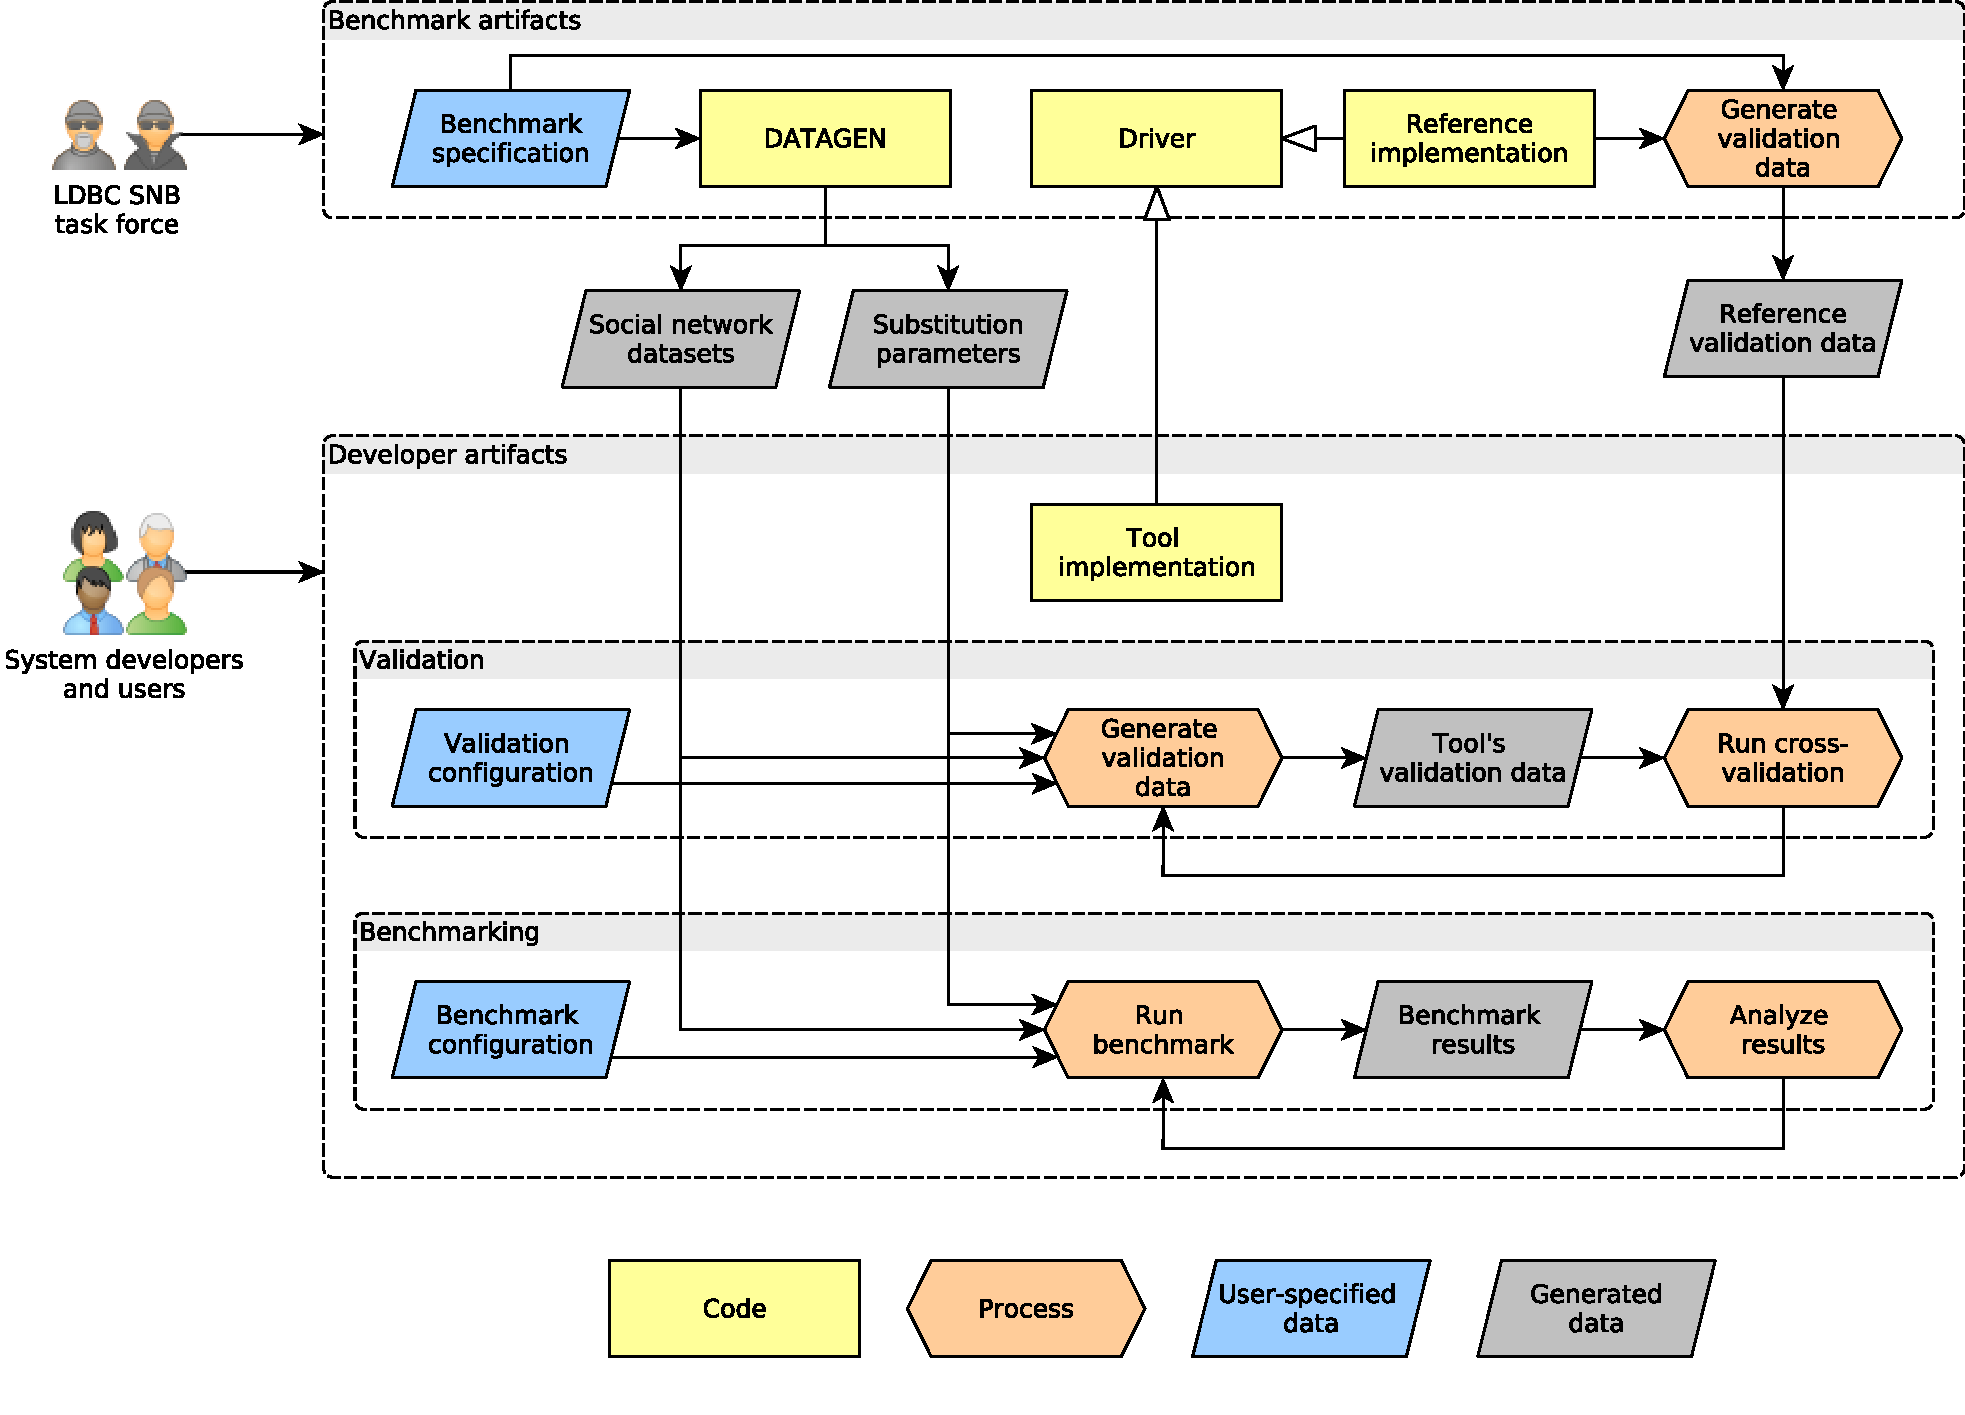
\includegraphics[width=\linewidth]{figures/workflow}
	\caption{Benchmark workflow.}
	\label{figure:workflow}
\end{figure}


\chapter{Workloads}
\label{section:workloads}

%%%%%%%%%%%%%%%%%%%%%%%%%%%%%%%%%%%%%%%%%%%%%%%%%%%%%%%%%%%%%%%%%%%%%%%%%%%%%%
%%%%%%%%%%%%%%%%%%%%%%%%%%%%%%%%%%%%%%%%%%%%%%%%%%%%%%%%%%%%%%%%%%%%%%%%%%%%%%
%%%%%%%%%%%%%%%%%%%%%%%%%%%%%%%%%%%%%%%%%%%%%%%%%%%%%%%%%%%%%%%%%%%%%%%%%%%%%%

\section{Query Description Format}
\label{sub:queries_structure}
Queries are described in natural language using a well-defined structure that consists of three sections:
\textit{description}, a concise textual description of the query;
\textit{parameters}, a list of input parameters and their types;
and \textit{results}, a list of expected results and their types.
The syntax used in \textit{parameters} and \textit{results} sections is as follows:

\begin{itemize}
    \item \textbf{Entity}: entity type in the dataset.\\
        One word, possibly constructed by appending multiple words together, starting with uppercase character and following the camel case notation,
        \eg \texttt{TagClass} represents an entity of type ``TagClass''.
    \item \textbf{Relationship}: relationship type in the dataset.\\
        One word, possibly constructed by appending multiple words together, starting with lowercase character and following the camel case notation,
        and surrounded by arrow to communicate direction,
        \eg \mbox{\texttt{-worksAt->}} represents a directed relationship of type ``worksAt''.
    \item \textbf{Attribute}: attribute of an entity or relationship in the dataset.\\
        One word, possibly constructed by appending multiple words together, starting with lowercase character and following the camel case notation,
        and prefixed by a ``.'' to dereference the entity/relationship,
        \eg \texttt{Person.firstName} refers to ``firstName'' attribute on the ``Person'' entity,
        and \mbox{\texttt{-studyAt->.classYear}} refers to ``classYear'' attribute on the ``studyAt'' relationship.
    \item \textbf{Unordered Set}: an unordered collection of distinct elements.\\
        Surrounded by \{ and \} braces, with the element type between them,
        \eg \texttt{\{String\}} refers to a set of strings.
    \item \textbf{Ordered List}: an ordered collection where duplicate elements are allowed.\\
        Surrounded by [ and ] braces, with the element type between them,
        \eg \texttt{[String]} refers to a list of strings.
    \item \textbf{Ordered Tuple}: a fixed length, fixed order list of elements, where elements at each position of the tuple have predefined, possibly different, types. \\
        Surrounded by < and > braces, with the element types between them in a specific order
        \eg \texttt{<String, Boolean>} refers to a 2-tuple containing a string value in the first element and a boolean value in the second,
        and \texttt{[<String, Boolean>]} is an ordered list of those 2-tuples.
\end{itemize}

\paragraph{Categorization of results.} Results are categorized according to their source of origin:

\begin{itemize}
	\item \textbf{Raw} (\texttt{R}), if the result is returned with an unmodified value and type.
	\item \textbf{Calculated} (\texttt{C}), if the result is calculated from other values and conditions.
	\item \textbf{Aggregated} (\texttt{A}), if the result is an aggregated value, \eg a count or a sum of another value. If a result is both calculated and aggregated (\eg $\mathsf{count(x) + count(y)}$ or $\mathsf{avg(x + y)}$), it is considered an aggregated result.
	\item \textbf{Meta} (\texttt{M}), if the result is based on type information, \eg the type of the node.
\end{itemize}


%%%%%%%%%%%%%%%%%%%%%%%%%%%%%%%%%%%%%%%%%%%%%%%%%%%%%%%%%%%%%%%%%%%%%%%%%%%%%%
%%%%%%%%%%%%%%%%%%%%%%%%%%%%%%%%%%%%%%%%%%%%%%%%%%%%%%%%%%%%%%%%%%%%%%%%%%%%%%
%%%%%%%%%%%%%%%%%%%%%%%%%%%%%%%%%%%%%%%%%%%%%%%%%%%%%%%%%%%%%%%%%%%%%%%%%%%%%%

\section{Conventions for Query Definitions}

\paragraph{Interval notations.} Closed interval boundaries are denoted with 
\texttt{[} 
and \texttt{]}, while open interval boundaries are denoted with \texttt{(} and 
\texttt{)}. For example, \texttt{[0, 1)} denoted an interval between 0 and 1, 
closed on the left and open on the right.

\paragraph{Comparing Date and DateTime values.}

Some query specifications (\eg \queryRefCard{bi-read-01}{BI}{1}, 
\queryRefCard{bi-read-02}{BI}{2}, etc.) require implementations to compare a 
$\mathsf{DateTime}$ value with a $\mathsf{Date}$ value. In these cases, the 
$\mathsf{Date}$ value should be implicitly converted $\mathsf{DateTime}$ value 
with a time of 00:00:00.000+0000 (\ie with the timezone of GMT).

\paragraph{Matching semantics.}

Unless noted otherwise, the specification uses \emph{homomorphic} matching 
semantics~\cite{Angles:2017:FMQ:3145473.3104031}, \ie both nodes and edges can 
occur multiple times in a match. Note that for variable length path, duplicate 
edges are not allowed.

\paragraph{Aggregation semantics.}

The \lstinline{count} aggregation always requires the query to determine the number of \emph{distinct} elements (nodes or edges). For example, this can be achieved in the Cypher, SPARQL and SQL query languages with the \lstinline[language=sql]{count(DISTINCT ...)} construct.

\paragraph{Graph patterns.}

To illustrate queries, we use graph patterns such as \autoref{fig:example-graph-pattern} with the following notation:

\begin{figure}[ht]
	\begin{center}
		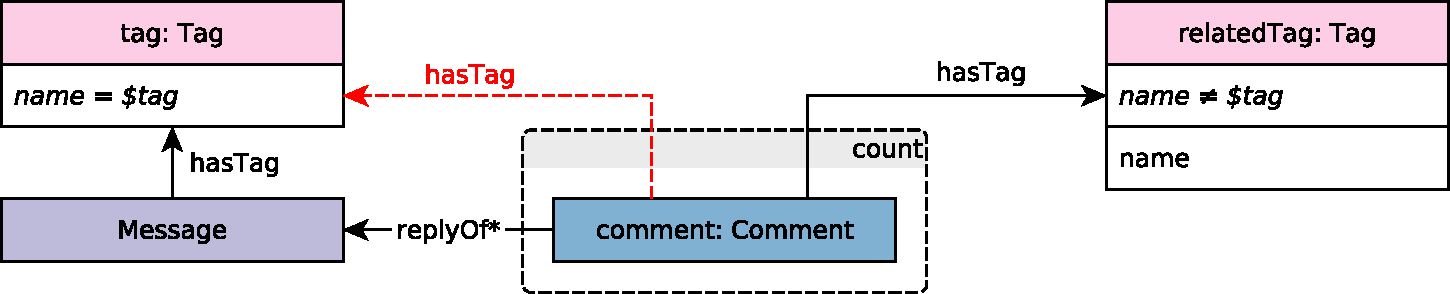
\includegraphics[scale=\patternscale,margin=0cm .2cm]{patterns/bi-read-08}
		\caption{Example graph pattern.}
		\label{fig:example-graph-pattern}
	\end{center}
\end{figure}

\begin{itemize}
	\item Nodes are marked as $\mathsf{entityName: EntityType}$ (camel case 
	notation for both, starting with a lowercase character for the first and an 
	uppercase character for the second). If the $\mathsf{entityName}$ is not used 
	in the query results, aggregations or calculations, and not referenced in the 
	query specification, the $\mathsf{entityName}$ can be omitted.
	\item Positive conditions for edges are denoted with solid lines.
	\item Negative conditions for edges, \ie edges that are not allowed in the graph, are denoted with \textcolor{red}{\dashuline{dashed red}} lines.
	\item Edges without direction imply that there must be an edge in \emph{at least one of the directions}.
	\item Filtering conditions are typeset in \textit{italic}, \eg $\mathit{id} = 
	\mathit{\textdollar tag}$.
	\item Attributes that should be returned are denoted in sans-serif font, \eg $\mathsf{name}$.
	\item Variable length paths, \ie edges that can be traversed multiple times 
	are denoted with $*\mathsf{min}...\mathsf{max}$, \eg $\mathsf{replyOf}*$ or 
	$\mathsf{knows*1 \ldots 2}$. By default, the value of $\mathsf{min}$ is 1, 
	and the value of $\mathsf{max}$ is unlimited.
	\item Aggregations are shown in dashed boxes with the type of aggregation ($\mathsf{count}$, $\mathsf{sum}$, $\mathsf{avg}$, etc.) in the upper right corner.
\end{itemize}

\newcommand{\tuple}[1]{\langle #1 \rangle}

\paragraph{Keywords.} The pattern notation uses a small set of keywords:

\begin{itemize}
	\item $\mathsf{UNWIND}$ unnests a list, \ie produces a set of one-tuples. For 
	example, $\mathsf{UNWIND} [1, 2, 3]$ results in $ \{ \tuple{1}, \tuple{2}, 
	\tuple{3} \} $.
	\item Aggregation operations: \lstinline{count}, \lstinline{avg}. % \lstinline{sum} - sum is not used in the figures as we always sum some derived value
	\item Functions:
	\begin{itemize}
		\item \lstinline{floor(x)} (returns $\lfloor x \rfloor$),
		\item \lstinline{year(date)} (extracts the year from a given date),
		\item \lstinline{month(date)} (extracts the month from a given date).
	\end{itemize}
\end{itemize}

\paragraph{Resolving ambiguity.} Note that if the textual description and the graph pattern are different for a particular query (either due to an error or the lack of sophistication in the graphical syntax), \emph{the textual description takes precedence}.

%%%%%%%%%%%%%%%%%%%%%%%%%%%%%%%%%%%%%%%%%%%%%%%%%%%%%%%%%%%%%%%%%%%%%%%%%%%%%%
%%%%%%%%%%%%%%%%%%%%%%%%%%%%%%%%%%%%%%%%%%%%%%%%%%%%%%%%%%%%%%%%%%%%%%%%%%%%%%
%%%%%%%%%%%%%%%%%%%%%%%%%%%%%%%%%%%%%%%%%%%%%%%%%%%%%%%%%%%%%%%%%%%%%%%%%%%%%%

\section{Substitution Parameters}

Together with the dataset, \datagen produces a set of parameters per
query type. Parameter generation is designed in such a way that for each query
type, all of the generated parameters yield similar runtime behaviour of that
query.

Specifically, the selection of parameters for a query template guarantees the following properties of the resulting queries:
\begin{enumerate}
\item[P1:] the query runtime has a bounded variance: the average runtime corresponds to the behavior of the majority of the queries
\item[P2:] the runtime distribution is stable: different samples of (\eg 10) parameter bindings used in different query streams result in an identical runtime distribution across streams
\item[P3:] the optimal logical plan (optimal operator order) of the queries is the same: this ensures that a specific query template tests the system's behavior under the well-chosen technical difficulty (\eg handling voluminous joins or proper cardinality estimation for subqueries, \etc)
\end{enumerate}


As a result, the amount of data that the query touches is roughly the
same for every parameter binding, assuming that the query optimizer figures out a
reasonable execution plan for the query. This is done to avoid bindings that
cause unexpectedly long or short runtimes of queries, or even result in a
completely different optimal execution plan. Such effects could arise due to
the data skew and correlations between values in the generated dataset.

In order to get the parameter bindings for each of the queries, we have designed a \textit{Parameter Curation} procedure that works in two stages:

\begin{enumerate}
\item for each query template for all possible parameter bindings, we determine the size of intermediate results in the {\em intended} query plan. Intermediate result size heavily influences the runtime of a query, so two queries with the same operator tree and similar intermediate result sizes at every level of this operator tree are expected to have similar runtimes. This analysis is effectively a side effect of data generation, that is we keep all the necessary counts (number of friends per user, number of posts of friends \etc) as we create the dataset.
\item then, a greedy algorithm selects (``curates'') those parameters with similar intermediate result counts from the domain of all the parameters.
\end{enumerate}

Parameter bindings are stored in the \texttt{substitution\_parameters} folder
inside the data generator directory. Each query gets its bindings in a separate
file. Every line of a parameter file is a JSON-formatted collection of
key-value pairs (name of the parameter and its value). For example, the Query 1
parameter bindings are stored in file \texttt{query\_1\_param.txt}, and one of
its lines may look like this:

\vspace{-6mm}
$$
\{\text{"PersonID"}: 1, \text{"Name"}: \text{"Lei"}, \text{"PersonURI"}: \text{"http://www.ldbc.eu/ldbc\_socialnet/1.0/data/pers1"}\}
$$

Depending on implementation, the SUT may refer to persons either by IDs
(relational and graph databases) or URIs (RDF systems), so we provide both
values for the Person parameter.  Finally, parameters for short reads are taken
from those in complex reads and updates.


%%%%%%%%%%%%%%%%%%%%%%%%%%%%%%%%%%%%%%%%%%%%%%%%%%%%%%%%%%%%%%%%%%%%%%%%%%%%%%
%%%%%%%%%%%%%%%%%%%%%%%%%%%%%%%%%%%%%%%%%%%%%%%%%%%%%%%%%%%%%%%%%%%%%%%%%%%%%%
%%%%%%%%%%%%%%%%%%%%%%%%%%%%%%%%%%%%%%%%%%%%%%%%%%%%%%%%%%%%%%%%%%%%%%%%%%%%%%

\section{Load Definition}

\ldbcsnb Test Driver is in charge of the execution of the Interactive Workload.
At the beginning of the execution, the Test Driver creates a query mix by
assigning to each query instance, a query issue time and a set of parameters
taken from the generated substitution parameter set described above.  

Query issue times have to be carefully assigned.  Although substitution
parameters are chosen in such a way that queries of the same type take similar
time, not all query types have the same complexity and touch the same amount of
data, which causes them to scale differently for the different scale factors.
Therefore, if all query instances, regardless of their type, are issued
at the same rate, those more complex queries will dominate the execution's
result, making faster query types purposeless. To avoid this situation, each
query type is executed at a different rate. The way the execution rate is decided,
also depends on the nature of the query: complex read, short read or update.

Update queries' issue times are taken from the update streams generated by the
data generator. These are the times where the actual event happened during the
simulation of the social network. Complex reads' times are expressed in terms
of update operations. For each complex read query type, a frequency value is
assigned which specifies the relation between the number of updates performed
per complex read.  Table~\ref{table:freqs} shows the frequencies assigned to
each query type for SF1. The frequencies of the different scale factors can be
found in Appendix~\ref{appendix:scale_factors}.

\begin{table}[H]
\centering
    \begin{tabular}{|c|c|c|c|}
    \hline
    Query Type & freq & Query Type & freq \\ 
    \hline
    \hline
    Query 1 & 26 & Query 8 & 45 \\ 
    \hline       
    Query 2 & 37 & Query 9 & 157 \\  
    \hline        
    Query 3 & 69 & Query 10 & 30 \\ 
    \hline        
    Query 4 & 36 & Query 11 & 16 \\ 
    \hline        
    Query 5 & 57 & Query 12 & 44 \\ 
    \hline        
    Query 6 & 129 & Query 13 & 19 \\  
    \hline        
    Query 7 & 87 & Query 14 & 49 \\ 
    \hline
    \end{tabular}
    \caption{Frequencies for each query type for SF1.}
    \label{table:freqs}
\end{table}

Finally, short reads are inserted in order to balance the ratio between reads
and writes, and to simulate the behavior of a real user of the social network.
For each complex read instance, a sequence of short reads is planned. There are two
types of short read sequences: Person centric and Message centric. Depending on
the type of the complex read, one of them is chosen. Each sequence consists of
a set of short reads which are issued in a row. The issue time assigned to each
short read in the sequence is determined at run time, and is based on the
completion time of the complex read it depends on. 
The substitution parameters for short reads are taken from the results of previously
executed complex reads and short reads.
Once a short read sequence is issued (and provided that sufficient substitution parameters 
exist), there is a probability that another short read  sequence is issued. 
This probability decreases for each new sequence issued. 
Since the same random number generator seed is used across
executions, the workload is deterministic.


The specified frequencies, implicitly define the query ratios between queries
of different types, as well as a default target throughput. However the Test
Sponsor may specify a different target throughput to test,  by ``squeezing''
together or ``stretching'' apart the queries of the workload. This is
achieved  by means of the ``Time Compression Ratio'' that is multiplied by the
frequencies (see \autoref{table:freqs}).  Therefore, different
throughputs can be tested while maintaining the relative ratios between the
different query types.


\chapter{Interactive Workload}

\section{Choke Points}

The design of the interactive workload queries has been conceived around two
main aspects: realism and technological relevance.  While realism has been
assessed by looking at existing social networks and thinking about what
interesting functionalities a user might desire from them, technological
relevance has been achieved by identifying a set of choke points queries should
stress.  These choke points capture those critical operations, techniques or
technologies that  could significatively affect the performance of the queries.
The choke points can be summarized in the following list:

% http://wiki.ldbcouncil.org/display/TUC/Interactive+Choke+Points

\subsection{Aggregation Performance}

The queries generally have a top-$k$ order by and often a group by in
addition to this.  These offer multiple optimization opportunities.
The queries also often have distinct operators, \ie distinct friends
within two steps.  Collectively these are all set operations that may
be implemented with some combination of hash and sorting, possibly
exploiting ordering in the data itself.  The aggregates are not
limited to counts and sums.  For example string concatenation occurs
as an aggregate, testing possible user defined aggregate support.
There is a wide range of cardinalities in grouping, from low, \eg country, to high, \eg post.

\subsection{Join Performance}

Each graph traversal step is in principle a join.  The join patterns are
diverse, exercising both index- and hash-based operators.   Queries are designed
so as to reward judicious use of hash join by having patterns starting with one
entity, fetching many related entities and then testing how these are related
to a third entity, \eg posts of a user with a tag of a given type.

\subsection{Data Access Locality}

Graph problems are notoriously non-local.  However, when queries touch
any non-trivial fraction of a dataset, locality will emerge and can be
exploited, for example by vectored index access or by ordering data so
that that a merge join is possible.

\subsection{Expression Calculation}

Queries often have expressions, including conditional expressions.
This provides opportunities for vectoring and tests efficient
management of intermediate results.

\subsection{Correlated Subqueries}

The workload has many correlated subqueries, for example constructts
like x within two steps but not in one step, which would typically be
a correlated subquery with NOT EXISTS.  There are also scalar
subqueries with aggregation, for example returning the count of posts
satisfying a certain criteria.


\subsection{Parallelism and Concurrency}

All queries offer opportunities for parallelism.  This tests a wide
range of constructs, for example partitioned parallel variants of
group by and distinct.  An interactive workload will typically avoid
trivially parallelizable table scans.  Thus the opportunities that
exist must be captured by index based, navigational query plans.  The
choice of whether to parallelize or not is often left to run time and
will have to depend on the actual data seen in the execution, as
starting a parallel thread with too little to do is
counter-productive.


\subsection{Graph Specifics}

Graph problems are generally characterized by transitive properties
and the fact that neighboring vertices often have a large overlap in
their environments.  This makes cardinality estimation harder.  For
example, a query optimizer needs to recognize whether a relationship
has a tree or graph shape in order to make correct cardinality
estimations.  Further, there are problems aggregating properties over
a set of consecutive edges.  The workload contains business questions
dealing with paths and aggregates across paths, as well as the easier
case of determining a membership in a hierarchy with a transitive
part-of relation.


\section{Query Specifications}

\subsection{Complex Reads Query Descriptions}
\label{sub:queries}

%\renewcommand*{\arraystretch}{1.1}

\subsection*{Interactive / complex / 1}
\label{section:interactive-complex-read-01}

\noindent\begin{tabularx}{\queryCardWidth}{|>{\queryPropertyCell}p{\queryPropertyCellWidth}|X|}
	\hline
	query & Interactive / complex / 1 \\ \hline
%
	title & Friends with certain name
 \\ \hline
%
	pattern & \hfill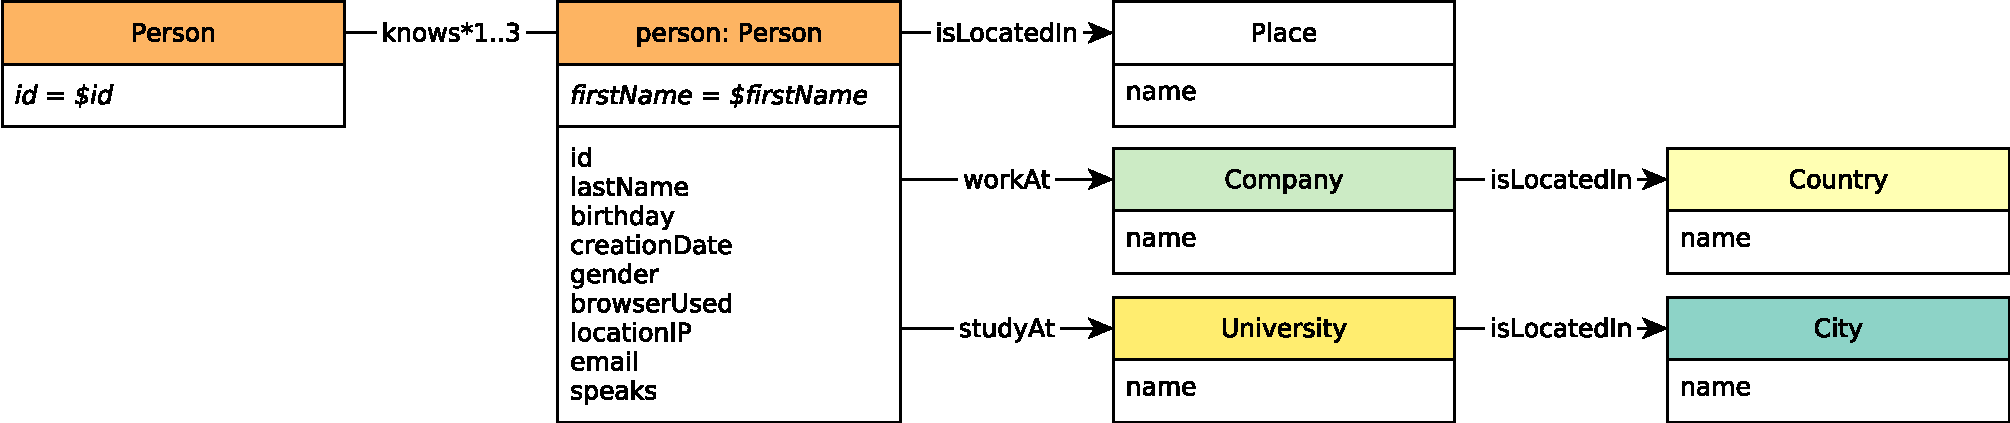
\includegraphics[scale=\patternscale,margin=0cm .2cm]{patterns/interactive-complex-read-01}\hfill\vadjust{} \\ \hline
%
	desc. & Given a start Person, find Persons with a given first name that the
start Person is connected to (excluding start Person) by at most 3 steps
via Knows relationships. Return Persons, including summaries of the
Persons workplaces and places of study.
 \\ \hline
%
	
		params &
		\innerCardVSpace{\begin{tabularx}{\attributeCardWidth}{|>{\paramNumberCell}c|>{\varNameCell}M|>{\typeCell}m{\typeWidth}|Y|} \hline
		$\mathsf{1}$ & Person.id
 & ID
 &  \\ \hline
		$\mathsf{2}$ & Person.firstName
 & String
 &  \\ \hline
		\end{tabularx}}\innerCardVSpace \\ \hline
	
%
	
		result &
		\innerCardVSpace{\begin{tabularx}{\attributeCardWidth}{|>{\resultNumberCell}c|>{\varNameCell}M|>{\typeCell}m{\typeWidth}|>{\resultOriginCell}c|Y|} \hline
		$\mathsf{1}$ & Person.id
 & ID
 & R &
				 \\ \hline
		$\mathsf{2}$ & Person.lastName
 & String
 & R &
				 \\ \hline
		$\mathsf{3}$ & Person.birthday
 & Date
 & R &
				 \\ \hline
		$\mathsf{4}$ & Person.creationDate
 & DateTime
 & R &
				 \\ \hline
		$\mathsf{5}$ & Person.gender
 & String
 & R &
				 \\ \hline
		$\mathsf{6}$ & Person.browserUsed
 & String
 & R &
				 \\ \hline
		$\mathsf{7}$ & Person.locationIP
 & String
 & R &
				 \\ \hline
		$\mathsf{8}$ & \{Person.email\}
 & \{String\}
 & R &
				 \\ \hline
		$\mathsf{9}$ & \{Person.speaks\}
 & \{String\}
 & R &
				 \\ \hline
		$\mathsf{10}$ & Person-isLocatedIn-\textgreater{}Place.name
 & String
 & R &
				 \\ \hline
		$\mathsf{11}$ & \{Person-studyAt-\textgreater{}University.name,
Person-studyAt-\textgreater{}.classYear,
Person-studyAt-\textgreater{}University-isLocatedIn-\textgreater{}City.name\}
 & \{\}
 & R &
				 \\ \hline
		$\mathsf{12}$ & \{Person-workAt-\textgreater{}Company.name,
Person-workAt-\textgreater{}.workFrom,
Person-workAt-\textgreater{}Company-isLocatedIn-\textgreater{}Country.name\}
 & \{\}
 & R &
				 \\ \hline
		\end{tabularx}}\innerCardVSpace \\ \hline
	
%
	
		sort		&
		\innerCardVSpace{\begin{tabularx}{\attributeCardWidth}{|>{\sortNumberCell}c|>{\varNameCell}M|>{\directionCell}c|Y|} \hline
		$\mathsf{1}$ & distanceFromPerson
 & $\asc
$ &  \\ \hline
		$\mathsf{2}$ & Person.lastName
 & $\asc
$ &  \\ \hline
		$\mathsf{3}$ & Person.id
 & $\asc
$ &  \\ \hline
		\end{tabularx}}\innerCardVSpace \\ \hline
	%
	limit & 20 \\ \hline
	%
	CPs &
	\multicolumn{1}{>{\raggedright}l|}{
		\chokePoint{1.3}, 
		\chokePoint{2.1}, 
		\chokePoint{5.3}
		} \\ \hline
	%
	relevance &
		\small This query is a representative of a simple navigational query. It looks for paths of length one, two or three through
the knows relation, starting from a given Person and ending at a Person with a given name. It is interesting for several
aspects. First, it requires for a complex aggregation, that is, returning the concatenation of universities, companies,
languages and email information of the person. Second, it tests the ability of the optimizer to move the evaluation of
sub-queries functionally dependant on the Person, after the evaluation of the top-k. Finally, performance is
highly sensitive to properly estimating the cardinalities in each transitive path, and paying attention not to explode
already visited Persons.
 \\ \hline%
\end{tabularx}
\queryCardVSpace
\renewcommand*{\arraystretch}{1.1}

\subsection*{Interactive / complex / 2}
\label{section:interactive-complex-read-02}

% change \emph{} to use sans-serif font
\let\oldemph\emph
\renewcommand{\emph}[1]{{\footnotesize \sf #1}}

\renewcommand{\currentQueryCard}{2}
\marginpar{
	\raggedleft
	\vspace{0.22ex}

	\queryRefCard{interactive-complex-read-01}{Interactive}{1}\\
	\queryRefCard{interactive-complex-read-02}{Interactive}{2}\\
	\queryRefCard{interactive-complex-read-03}{Interactive}{3}\\
	\queryRefCard{interactive-complex-read-04}{Interactive}{4}\\
	\queryRefCard{interactive-complex-read-05}{Interactive}{5}\\
	\queryRefCard{interactive-complex-read-06}{Interactive}{6}\\
	\queryRefCard{interactive-complex-read-07}{Interactive}{7}\\
	\queryRefCard{interactive-complex-read-08}{Interactive}{8}\\
	\queryRefCard{interactive-complex-read-09}{Interactive}{9}\\
	\queryRefCard{interactive-complex-read-10}{Interactive}{10}\\
	\queryRefCard{interactive-complex-read-11}{Interactive}{11}\\
	\queryRefCard{interactive-complex-read-12}{Interactive}{12}\\
	\queryRefCard{interactive-complex-read-13}{Interactive}{13}\\
	\queryRefCard{interactive-complex-read-14}{Interactive}{14}\\
}

\noindent\begin{tabularx}{\queryCardWidth}{|>{\queryPropertyCell}p{\queryPropertyCellWidth}|X|}
	\hline
	query & Interactive / complex / 2 \\ \hline
%
	title & Recent posts and comments by your friends \\ \hline
%
	pattern & \multicolumn{1}{c|}{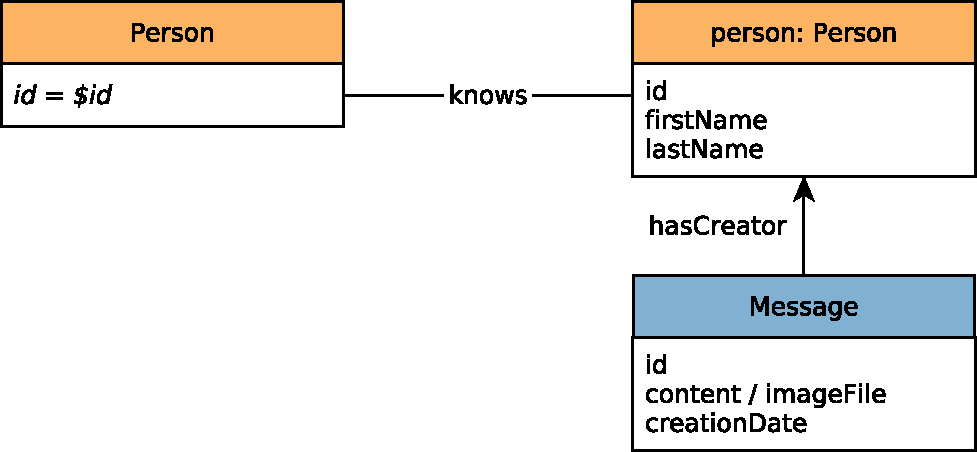
\includegraphics[scale=\patternscale,margin=0cm .2cm]{patterns/interactive-complex-read-02}} \\ \hline
%
	desc. & Given a start Person, find (most recent) Messages from all of that
Person's friends, that were created before (and including) a given date.
 \\ \hline
%
	
		params &
		\innerCardVSpace{\begin{tabularx}{\attributeCardWidth}{|>{\paramNumberCell}c|>{\varNameCell}M|>{\typeCell}m{\typeWidth}|Y|} \hline
		$\mathsf{1}$ & Person.id
 & ID
 &  \\ \hline
		$\mathsf{2}$ & date
 & DateTime
 &  \\ \hline
		\end{tabularx}}\innerCardVSpace \\ \hline
	
%
	
		result &
		\innerCardVSpace{\begin{tabularx}{\attributeCardWidth}{|>{\resultNumberCell}c|>{\varNameCell}M|>{\typeCell}m{\typeWidth}|>{\resultOriginCell}c|Y|} \hline
		$\mathsf{1}$ & Message-hasCreator-\textgreater{}Person.id & ID & R &
				 \\ \hline
		$\mathsf{2}$ & Message-hasCreator-\textgreater{}Person.firstName & String & R &
				 \\ \hline
		$\mathsf{3}$ & Message-hasCreator-\textgreater{}Person.lastName & String & R &
				 \\ \hline
		$\mathsf{4}$ & Message.id & ID & R &
				 \\ \hline
		$\mathsf{5}$ & Message.content or Post.imageFile & String & R &
				 \\ \hline
		$\mathsf{6}$ & Message.creationDate & DateTime & R &
				 \\ \hline
		\end{tabularx}}\innerCardVSpace \\ \hline
	
%
	
		sort		&
		\innerCardVSpace{\begin{tabularx}{\attributeCardWidth}{|>{\sortNumberCell}c|>{\varNameCell}M|>{\directionCell}c|Y|} \hline
		$\mathsf{1}$ & Message.creationDate
 & $\desc
$ &  \\ \hline
		$\mathsf{2}$ & Message.id
 & $\asc
$ &  \\ \hline
		\end{tabularx}}\innerCardVSpace \\ \hline
	%
	limit & 20 \\ \hline
	%
	CPs &
	\multicolumn{1}{>{\raggedright}l|}{
		\chokePoint{1.1}, 
		\chokePoint{2.2}, 
		\chokePoint{2.3}, 
		\chokePoint{3.2}
		} \\ \hline
	%
	relevance &
		\small This is a navigational query looking for paths of length two, starting from a given Person, going to their friends and
from them, moving to their published Posts and Comments. This query exercices both the optimizer and how data is
stored. It tests the ability to create execution plans taking advantage of the orderings induced by some operators to
avoid performing expensive sorts. This query requires selecting Posts and Comments based on their creation date,
which might be correlated with their identifier and therefore, having intermediate results with interesting orders.
Also, messages could be stored in an order correlated with their creation date to improve data access locality. Finally,
as many of the attributes required in the projection are not needed for the execution of the query, it is expected that
the query optimizer will move the projection to the end.
 \\ \hline%
\end{tabularx}
\queryCardVSpace

% change \emph back to the old one
\renewcommand{\emph}[1]{\oldemph{#1}}
\renewcommand*{\arraystretch}{1.1}

\subsection*{Interactive / complex / 3}
\label{section:interactive-complex-read-03}

% change \emph{} to use sans-serif font
\let\oldemph\emph
\renewcommand{\emph}[1]{{\footnotesize \sf #1}}

\renewcommand{\currentQueryCard}{3}
\marginpar{
	\raggedleft
	\vspace{0.22ex}

	\queryRefCard{interactive-complex-read-01}{IC}{1}\\
	\queryRefCard{interactive-complex-read-02}{IC}{2}\\
	\queryRefCard{interactive-complex-read-03}{IC}{3}\\
	\queryRefCard{interactive-complex-read-04}{IC}{4}\\
	\queryRefCard{interactive-complex-read-05}{IC}{5}\\
	\queryRefCard{interactive-complex-read-06}{IC}{6}\\
	\queryRefCard{interactive-complex-read-07}{IC}{7}\\
	\queryRefCard{interactive-complex-read-08}{IC}{8}\\
	\queryRefCard{interactive-complex-read-09}{IC}{9}\\
	\queryRefCard{interactive-complex-read-10}{IC}{10}\\
	\queryRefCard{interactive-complex-read-11}{IC}{11}\\
	\queryRefCard{interactive-complex-read-12}{IC}{12}\\
	\queryRefCard{interactive-complex-read-13}{IC}{13}\\
	\queryRefCard{interactive-complex-read-14}{IC}{14}\\
}


\noindent\begin{tabularx}{\queryCardWidth}{|>{\queryPropertyCell}p{\queryPropertyCellWidth}|X|}
	\hline
	query & Interactive / complex / 3 \\ \hline
%
	title & Friends and friends of friends that have been to countries X and Y \\ \hline
%
	pattern & \multicolumn{1}{c|}{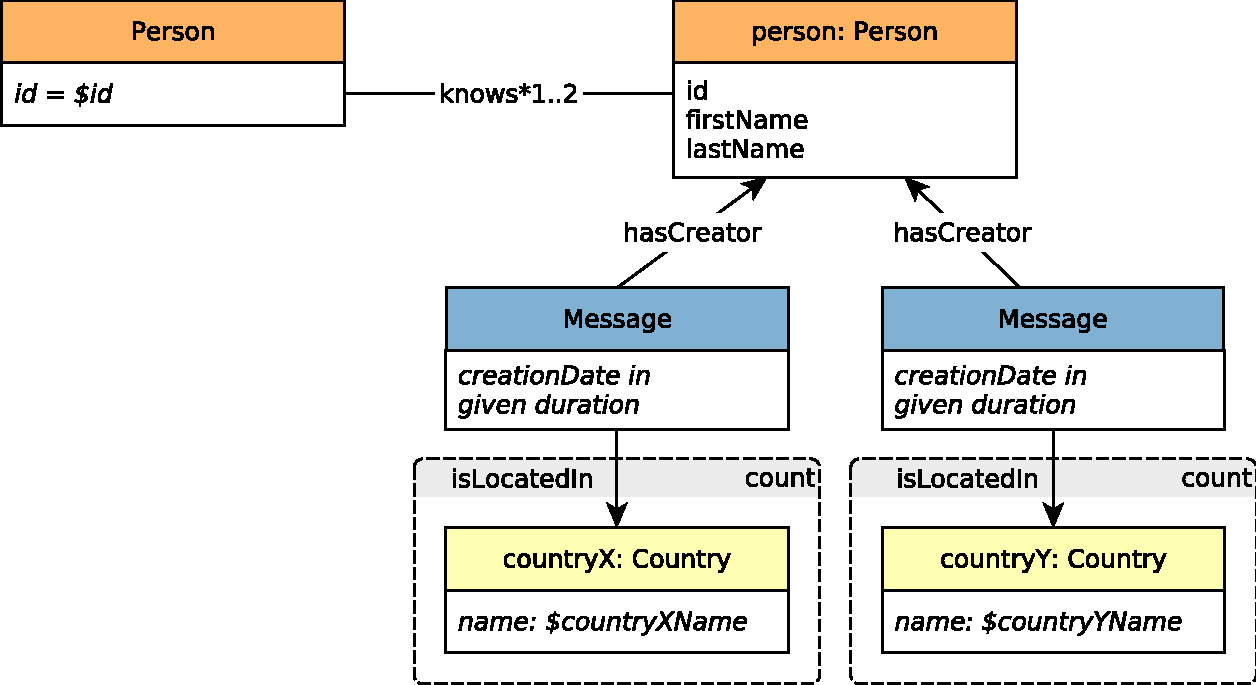
\includegraphics[scale=\patternscale,margin=0cm .2cm]{patterns/interactive-complex-read-03}} \\ \hline
%
	desc. & Given a start Person, find Persons that are their friends and friends of
friends (excluding start Person) that have made Posts/Comments in both
of the given Countries, X and Y, within a given period. Only Persons
that are foreign to Countries X and Y are considered, that is Persons
whose Location is not Country X or Country Y.
 \\ \hline
%
	
		params &
		\innerCardVSpace{\begin{tabularx}{\attributeCardWidth}{|>{\paramNumberCell}c|>{\varNameCell}M|>{\typeCell}m{\typeWidth}|Y|} \hline
		$\mathsf{1}$ & Person.id
 & ID
 &  \\ \hline
		$\mathsf{2}$ & CountryX.name
 & String
 &  \\ \hline
		$\mathsf{3}$ & CountryY.name
 & String
 &  \\ \hline
		$\mathsf{4}$ & startDate
 & Date
 & Beginning of requested period
 \\ \hline
		$\mathsf{5}$ & duration
 & 32-bit Integer
 & Duration of requested period, in days the interval {[}startDate,
startDate + Duration) is closed-open
 \\ \hline
		\end{tabularx}}\innerCardVSpace \\ \hline
	
%
	
		result &
		\innerCardVSpace{\begin{tabularx}{\attributeCardWidth}{|>{\resultNumberCell}c|>{\varNameCell}M|>{\typeCell}m{\typeWidth}|>{\resultOriginCell}c|Y|} \hline
		$\mathsf{1}$ & Person.id & ID & R &
				 \\ \hline
		$\mathsf{2}$ & Person.firstName & String & R &
				 \\ \hline
		$\mathsf{3}$ & Person.lastName & String & R &
				 \\ \hline
		$\mathsf{4}$ & countX & 32-bit Integer & A &
				Number of Messages from Country X made by Person within the given time
 \\ \hline
		$\mathsf{5}$ & countY & 32-bit Integer & A &
				Number of Messages from Country Y made by Person within the given time
 \\ \hline
		$\mathsf{6}$ & count & 32-bit Integer & A &
				\texttt{countX} + \texttt{countY}
 \\ \hline
		\end{tabularx}}\innerCardVSpace \\ \hline
	
%
	
		sort		&
		\innerCardVSpace{\begin{tabularx}{\attributeCardWidth}{|>{\sortNumberCell}c|>{\varNameCell}M|>{\directionCell}c|Y|} \hline
		$\mathsf{1}$ & countX
 & $\desc
$ &  \\ \hline
		$\mathsf{2}$ & Person.id
 & $\asc
$ &  \\ \hline
		\end{tabularx}}\innerCardVSpace \\ \hline
	%
	limit & 20 \\ \hline
	%
	CPs &
	\multicolumn{1}{>{\raggedright}l|}{
		\chokePoint{2.1}, 
		\chokePoint{3.1}, 
		\chokePoint{5.1}
		} \\ \hline
	%
	relevance &
		\small This query looks for paths of length two and three, starting from a Person, going to friends or friends of friends, and
then moving to Messages. This query tests the ability of the query optimizer to select the most efficient join ordering,
which will depend on the cardinalities of the intermediate results. Many friends of friends can be duplicate, then it is
expected to eliminate duplicates and those people prior to access the Post and Comments, as well as eliminate those
friends from countries X and Y, as the size of the intermediate results can be severely affected. A possible structural
optimization could be to materialize the number of Posts and Comments created by a person, and progressively
filter those people that could not even fall in the top 20 even having all their posts in the countries X and Y.
 \\ \hline%
\end{tabularx}
\queryCardVSpace

% change \emph back to the old one
\let\emph\oldemph
\renewcommand*{\arraystretch}{1.1}

\subsection*{Interactive / complex / 4}
\label{section:interactive-complex-read-04}

% change \emph{} to use sans-serif font
\let\oldemph\emph
\renewcommand{\emph}[1]{{\footnotesize \sf #1}}

\renewcommand{\currentQueryCard}{4}
\marginpar{
	\raggedleft
	\vspace{0.22ex}

	\queryRefCard{interactive-complex-read-01}{IC}{1}\\
	\queryRefCard{interactive-complex-read-02}{IC}{2}\\
	\queryRefCard{interactive-complex-read-03}{IC}{3}\\
	\queryRefCard{interactive-complex-read-04}{IC}{4}\\
	\queryRefCard{interactive-complex-read-05}{IC}{5}\\
	\queryRefCard{interactive-complex-read-06}{IC}{6}\\
	\queryRefCard{interactive-complex-read-07}{IC}{7}\\
	\queryRefCard{interactive-complex-read-08}{IC}{8}\\
	\queryRefCard{interactive-complex-read-09}{IC}{9}\\
	\queryRefCard{interactive-complex-read-10}{IC}{10}\\
	\queryRefCard{interactive-complex-read-11}{IC}{11}\\
	\queryRefCard{interactive-complex-read-12}{IC}{12}\\
	\queryRefCard{interactive-complex-read-13}{IC}{13}\\
	\queryRefCard{interactive-complex-read-14}{IC}{14}\\
}


\noindent\begin{tabularx}{\queryCardWidth}{|>{\queryPropertyCell}p{\queryPropertyCellWidth}|X|}
	\hline
	query & Interactive / complex / 4 \\ \hline
%
	title & New topics \\ \hline
%
	pattern & \multicolumn{1}{c|}{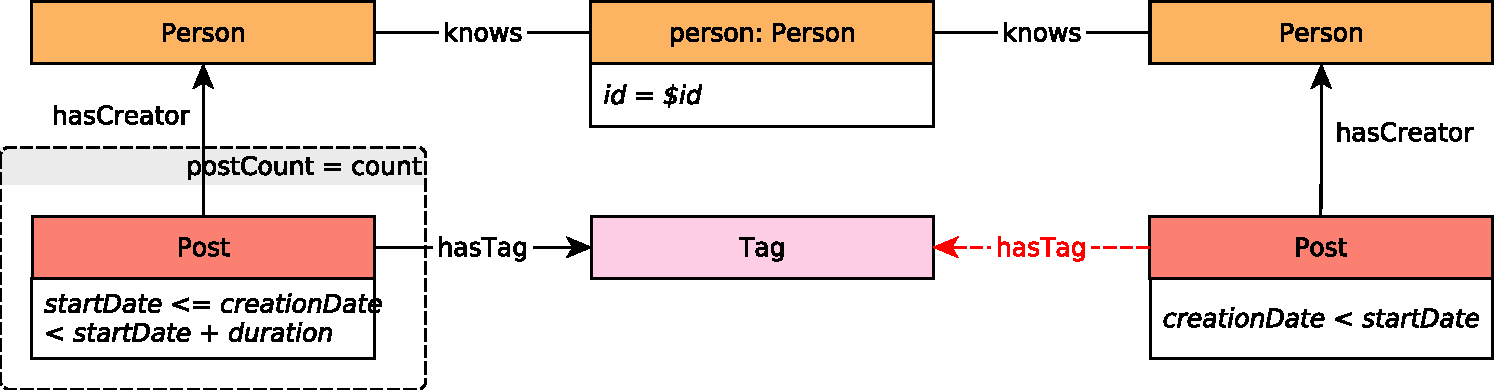
\includegraphics[scale=\patternscale,margin=0cm .2cm]{patterns/interactive-complex-read-04}} \\ \hline
%
	desc. & Given a start Person, find Tags that are attached to Posts that were
created by that Person's friends. Only include Tags that were attached
to friends' Posts created within a given time interval, and that were
never attached to friends' Posts created before this interval.
 \\ \hline
%
	
		params &
		\innerCardVSpace{\begin{tabularx}{\attributeCardWidth}{|>{\paramNumberCell}c|>{\varNameCell}M|>{\typeCell}m{\typeWidth}|Y|} \hline
		$\mathsf{1}$ & Person.id
 & ID
 &  \\ \hline
		$\mathsf{2}$ & startDate
 & Date
 &  \\ \hline
		$\mathsf{3}$ & duration
 & 32-bit Integer
 & Duration of requested period, in days the interval {[}startDate,
startDate + Duration) is closed-open
 \\ \hline
		\end{tabularx}}\innerCardVSpace \\ \hline
	
%
	
		result &
		\innerCardVSpace{\begin{tabularx}{\attributeCardWidth}{|>{\resultNumberCell}c|>{\varNameCell}M|>{\typeCell}m{\typeWidth}|>{\resultOriginCell}c|Y|} \hline
		$\mathsf{1}$ & Tag.name & String & R &
				 \\ \hline
		$\mathsf{2}$ & count & 32-bit Integer & A &
				Number of Posts made within the given time interval that have this Tag
 \\ \hline
		\end{tabularx}}\innerCardVSpace \\ \hline
	
%
	
		sort		&
		\innerCardVSpace{\begin{tabularx}{\attributeCardWidth}{|>{\sortNumberCell}c|>{\varNameCell}M|>{\directionCell}c|Y|} \hline
		$\mathsf{1}$ & count
 & $\desc
$ &  \\ \hline
		$\mathsf{2}$ & Tag.name
 & $\asc
$ &  \\ \hline
		\end{tabularx}}\innerCardVSpace \\ \hline
	%
	limit & 10 \\ \hline
	%
	CPs &
	\multicolumn{1}{>{\raggedright}l|}{
		\chokePoint{2.3}
		} \\ \hline
	%
	relevance &
		\small This query looks for paths of length two, starting from a given Person, moving to Posts and then to Tags. It tests
the ability of the query optimizer to properly select the usage of hash joins or index based joins, depending on the
cardinality of the intermediate results. These cardinalities are clearly affected by the input Person, the number of
friends, the variety of Tags, the time interval and the number of Posts.
 \\ \hline%
\end{tabularx}
\queryCardVSpace

% change \emph back to the old one
\let\emph\oldemph
\renewcommand*{\arraystretch}{1.1}

\subsection*{Interactive / complex / 5}
\label{section:interactive-complex-read-05}

% change \emph{} to use sans-serif font
\let\oldemph\emph
\renewcommand{\emph}[1]{{\footnotesize \sf #1}}

\renewcommand{\currentQueryCard}{5}
\input{query-cards/interactive-navbar}

\noindent\begin{tabularx}{\queryCardWidth}{|>{\queryPropertyCell}p{\queryPropertyCellWidth}|X|}
	\hline
	query & Interactive / complex / 5 \\ \hline
%
	title & New groups
 \\ \hline
%
	pattern & \hfill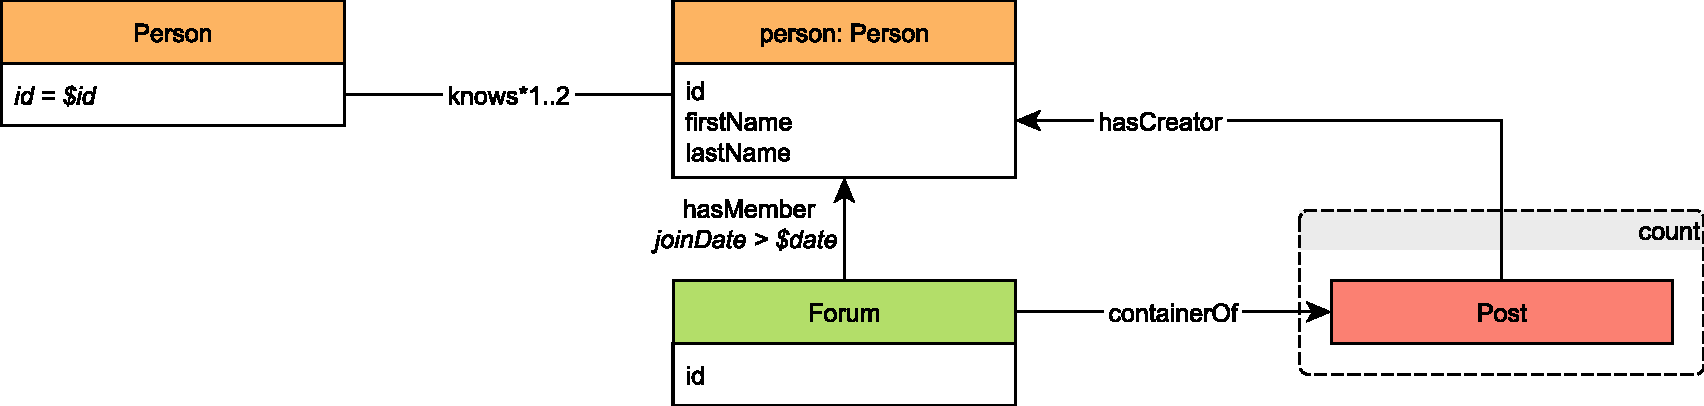
\includegraphics[scale=\patternscale,margin=0cm .2cm]{patterns/interactive-complex-read-05}\hfill\vadjust{} \\ \hline
%
	desc. & Given a start Person, find the Forums which that Person's friends and
friends of friends (excluding start Person) became Members of after a
given date. For each forum find the number of Posts that were created by
any of these Persons. For each Forum and consider only those Persons
which joined that particular Forum after the given date.
 \\ \hline
%
	
		params &
		\innerCardVSpace{\begin{tabularx}{\attributeCardWidth}{|>{\paramNumberCell}c|>{\varNameCell}M|>{\typeCell}m{\typeWidth}|Y|} \hline
		$\mathsf{1}$ & Person.id
 & ID
 &  \\ \hline
		$\mathsf{2}$ & date
 & Date
 &  \\ \hline
		\end{tabularx}}\innerCardVSpace \\ \hline
	
%
	
		result &
		\innerCardVSpace{\begin{tabularx}{\attributeCardWidth}{|>{\resultNumberCell}c|>{\varNameCell}M|>{\typeCell}m{\typeWidth}|>{\resultOriginCell}c|Y|} \hline
		$\mathsf{1}$ & Forum.title & String & R &
				 \\ \hline
		$\mathsf{2}$ & count & 32-bit Integer & A &
				Number of Posts made in Forum that were created by friends
 \\ \hline
		\end{tabularx}}\innerCardVSpace \\ \hline
	
%
	
		sort		&
		\innerCardVSpace{\begin{tabularx}{\attributeCardWidth}{|>{\sortNumberCell}c|>{\varNameCell}M|>{\directionCell}c|Y|} \hline
		$\mathsf{1}$ & count
 & $\desc
$ &  \\ \hline
		$\mathsf{2}$ & Forum.id
 & $\asc
$ &  \\ \hline
		\end{tabularx}}\innerCardVSpace \\ \hline
	%
	limit & 20 \\ \hline
	%
	CPs &
	\multicolumn{1}{>{\raggedright}l|}{
		\chokePoint{2.3}, 
		\chokePoint{3.3}
		} \\ \hline
	%
	relevance &
		\small This query looks for paths of length two and three, starting from a given Person, moving to friends and friends of
friends, and then getting the Forums they are members of. Besides testing the ability of the query optimizer to select
the proper join operator, it rewards the usage of indexes, but their accesses will be presumably scattered due to the
two/three-hop search space of the query, leading to unpredictable and scattered index accesses. Having efficient
implementations of such indexes will be highly beneficial.
 \\ \hline%
\end{tabularx}
\queryCardVSpace

% change \emph back to the old one
\renewcommand{\emph}[1]{\oldemph{#1}}
\renewcommand*{\arraystretch}{1.1}

\label{sec:interactive-complex-read-06}
\noindent\begin{tabularx}{\queryCardWidth}{|>{\queryPropertyCell}c|X|}
	\hline
	query & Interactive / complex / 6 \\ \hline
%
	title & Tag co-occurrence \\ \hline
%
    pattern & \hfill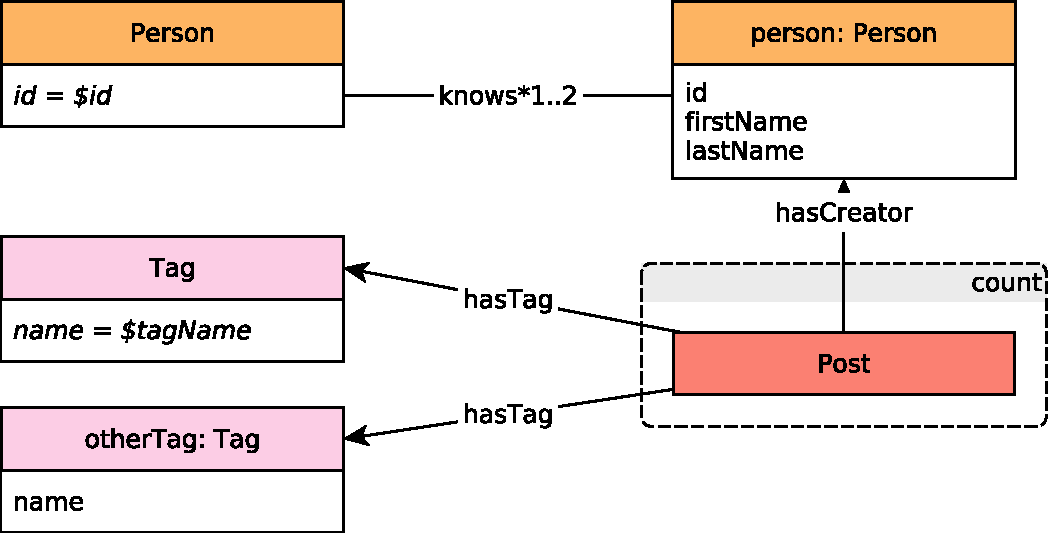
\includegraphics[scale=\patternscale,margin=0cm .2cm]{patterns/interactive-complex-read-06}\hfill\vadjust{} \\ \hline
%
	desc. & Given a start Person and some Tag, find the other Tags that occur
together with this Tag on Posts that were created by start Person's
friends and friends of friends (excluding start Person). Return For each
Tag, find the count of Posts that were created by these Persons, which
contain both this Tag and the given Tag.
 \\ \hline
%
	
%
    
        params &
        \innerCardVSpace{\begin{tabularx}{\attributeCardWidth}{|>{\paramNumberCell}c|>{\varNameCell}M|>{\typeCell}m{\typeWidth}|Y|} \hline
        \cellcolor{parameter} \color{white} \footnotesize $\mathsf{1}$ &Person.id& ID &  \\ \hline
        \cellcolor{parameter} \color{white} \footnotesize $\mathsf{2}$ &Tag.name& String &  \\ \hline
        \end{tabularx}}\innerCardVSpace \\ \hline
	
%
	
        result &
        \innerCardVSpace{\begin{tabularx}{\attributeCardWidth}{|>{\resultNumberCell}c|>{\varNameCell}M|>{\typeCell}m{\typeWidth}|>{\resultOriginCell}c|Y|} \hline
        $\mathsf{1}$ & Tag.name & String &R&
                 \\ \hline
        $\mathsf{2}$ & count & 32-bit Integer &A&
                number of Posts that were created by friends and friends of friends, which contain this Tag \\ \hline
        \end{tabularx}}\innerCardVSpace \\ \hline
	
%
	sort        &
        \innerCardVSpace{\begin{tabular}{|>{\sortNumberCell}c|>{\varNameCell}l|>{\directionCell}c|} \hline
        $\mathsf{1}$ & count & $\desc$ \\ \hline
        $\mathsf{2}$ & Tag.name & $\asc$ \\ \hline
        \end{tabular}}\innerCardVSpace \\ \hline
	%
	limit & 10 \\ \hline
	%
	CPs &
	\multicolumn{1}{>{\raggedright}l|}{
	    \chokePoint{5.1}
	    } \\ \hline
	%
    relevance &
        \small This query looks for paths of lengths three or four, starting from a Given Person, moving to friends or friends of
friends, then to Posts and finally ending at a given Tag.
 \\ \hline%
\end{tabularx}
\queryCardVSpace
\renewcommand*{\arraystretch}{1.1}

\subsection*{Interactive / complex / 7}
\label{section:interactive-complex-read-07}

\noindent\begin{tabularx}{\queryCardWidth}{|>{\queryPropertyCell}p{\queryPropertyCellWidth}|X|}
	\hline
	query & Interactive / complex / 7 \\ \hline
%
	title & Recent likers
 \\ \hline
%
	pattern & \hfill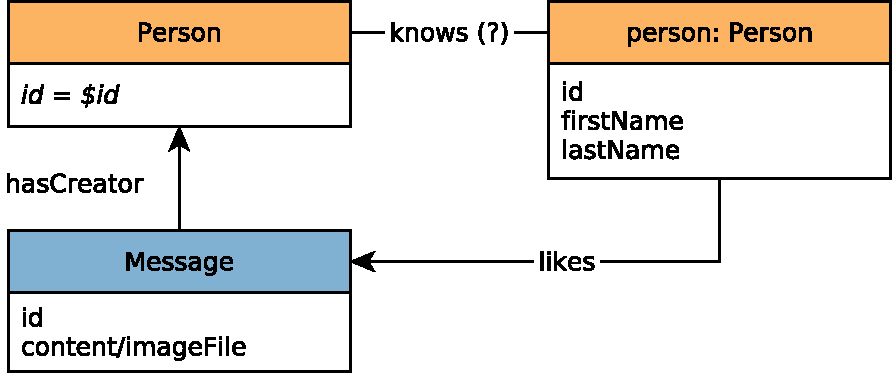
\includegraphics[scale=\patternscale,margin=0cm .2cm]{patterns/interactive-complex-read-07}\hfill\vadjust{} \\ \hline
%
	desc. & Given a start Person, find (most recent) Likes on any of start Person's
Messages. Find Persons that Liked any of start Person's Messages, the
Messages they liked most recently, creation date of that Like, and the
latency (in minutes) between creation of Messages and Like.
Additionally, for each Person found return a flag indicating whether the
liker is a friend of start Person. In the case that a Person Liked
multiple Messages at the same time, return the Message with lowest
identifier.
 \\ \hline
%
	
		params &
		\innerCardVSpace{\begin{tabularx}{\attributeCardWidth}{|>{\paramNumberCell}c|>{\varNameCell}M|>{\typeCell}m{\typeWidth}|Y|} \hline
		$\mathsf{1}$ & Person.id
 & 64-bit Integer
 &  \\ \hline
		\end{tabularx}}\innerCardVSpace \\ \hline
	
%
	
		result &
		\innerCardVSpace{\begin{tabularx}{\attributeCardWidth}{|>{\resultNumberCell}c|>{\varNameCell}M|>{\typeCell}m{\typeWidth}|>{\resultOriginCell}c|Y|} \hline
		$\mathsf{1}$ & Person.id
 & ID
 & R &
				 \\ \hline
		$\mathsf{2}$ & Person.firstName
 & String
 & R &
				 \\ \hline
		$\mathsf{3}$ & Person.lastName
 & String
 & R &
				 \\ \hline
		$\mathsf{4}$ & Like.creationDate
 & DateTime
 & R &
				 \\ \hline
		$\mathsf{5}$ & Message.id
 & ID
 & R &
				 \\ \hline
		$\mathsf{6}$ & Message.content or Post.imageFile
 & String
 & R &
				 \\ \hline
		$\mathsf{7}$ & latency
 & 32-bit Integer
 & R &
				Duration between creation of Message and Like, in minutes
 \\ \hline
		$\mathsf{8}$ & isNew
 & Boolean
 & R &
				\texttt{false} if liker Person is friend of start Person, \texttt{true}
otherwise
 \\ \hline
		\end{tabularx}}\innerCardVSpace \\ \hline
	
%
	
		sort		&
		\innerCardVSpace{\begin{tabularx}{\attributeCardWidth}{|>{\sortNumberCell}c|>{\varNameCell}M|>{\directionCell}c|Y|} \hline
		$\mathsf{1}$ & Like.creationDate
 & $\desc
$ &  \\ \hline
		$\mathsf{2}$ & Person.id
 & $\asc
$ &  \\ \hline
		\end{tabularx}}\innerCardVSpace \\ \hline
	%
	limit & 20 \\ \hline
	%
	CPs &
	\multicolumn{1}{>{\raggedright}l|}{
		\chokePoint{2.2}, 
		\chokePoint{2.3}, 
		\chokePoint{3.3}, 
		\chokePoint{5.1}
		} \\ \hline
	%
	relevance &
		\small This query looks for paths of length two, starting from a given Person, moving
to its published messages and then to Persons who liked them. It tests several aspects related to join optimization,
both at query optimization plan level and execution engine level. On the one hand, many of the columns needed for
the projection are only needed in the last stages of the query, so the optimizer is expected to delay the projection
until the end. This query implies accessing 2-hop data, and as a consequence, index accesses are expected to be
scattered. We expect to observe variate cardinalities, depending on the characteristics of the input parameter, so
properly selecting the join operators will be crucial. This query has a lot of correlated sub-queries, so it is testing
the ability to flatten the query execution plans.
 \\ \hline%
\end{tabularx}
\queryCardVSpace
\renewcommand*{\arraystretch}{1.1}

\subsection*{Interactive / complex / 8}
\label{section:interactive-complex-read-08}

% change \emph{} to use sans-serif font
\let\oldemph\emph
\renewcommand{\emph}[1]{{\footnotesize \sf #1}}

\renewcommand{\currentQueryCard}{8}
\marginpar{
	\raggedleft
	\vspace{0.22ex}

	\queryRefCard{interactive-complex-read-01}{IC}{1}\\
	\queryRefCard{interactive-complex-read-02}{IC}{2}\\
	\queryRefCard{interactive-complex-read-03}{IC}{3}\\
	\queryRefCard{interactive-complex-read-04}{IC}{4}\\
	\queryRefCard{interactive-complex-read-05}{IC}{5}\\
	\queryRefCard{interactive-complex-read-06}{IC}{6}\\
	\queryRefCard{interactive-complex-read-07}{IC}{7}\\
	\queryRefCard{interactive-complex-read-08}{IC}{8}\\
	\queryRefCard{interactive-complex-read-09}{IC}{9}\\
	\queryRefCard{interactive-complex-read-10}{IC}{10}\\
	\queryRefCard{interactive-complex-read-11}{IC}{11}\\
	\queryRefCard{interactive-complex-read-12}{IC}{12}\\
	\queryRefCard{interactive-complex-read-13}{IC}{13}\\
	\queryRefCard{interactive-complex-read-14}{IC}{14}\\
}


\noindent\begin{tabularx}{\queryCardWidth}{|>{\queryPropertyCell}p{\queryPropertyCellWidth}|X|}
	\hline
	query & Interactive / complex / 8 \\ \hline
%
	title & Recent replies \\ \hline
%
	pattern & \centering 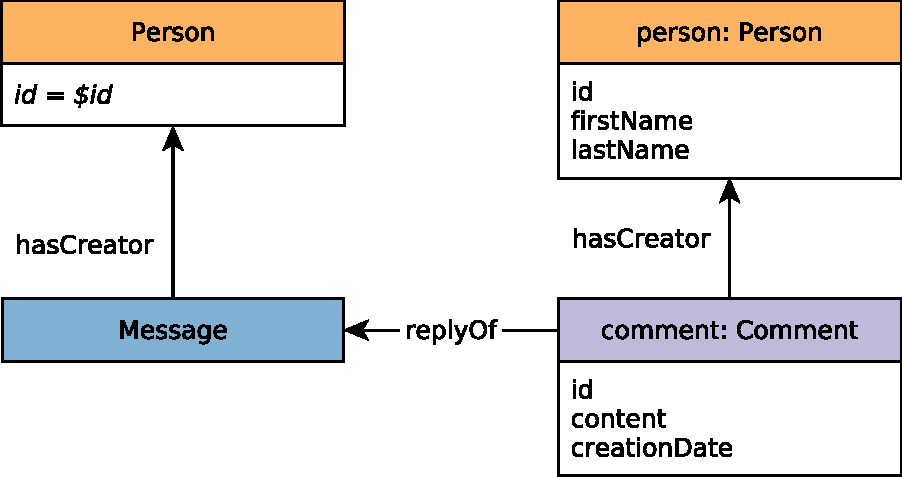
\includegraphics[scale=\patternscale,margin=0cm .2cm]{patterns/interactive-complex-read-08} \tabularnewline \hline
%
	desc. & Given a start \emph{Person}, find (most recent) \emph{Comments} that are
replies to \emph{Messages} of the start \emph{Person}. Only consider
direct (single-hop) replies, not the transitive (multi-hop) ones. Return
the reply \emph{Comments}, and the \emph{Person} that created each reply
\emph{Comment}.
 \\ \hline
%
	
		params &
		\innerCardVSpace{\begin{tabularx}{\attributeCardWidth}{|>{\paramNumberCell}c|>{\varNameCell}M|>{\typeCell}m{\typeWidth}|Y|} \hline
		$\mathsf{1}$ & Person.id
 & ID
 & \texttt{personId}
 \\ \hline
		\end{tabularx}}\innerCardVSpace \\ \hline
	
%
	
		result &
		\innerCardVSpace{\begin{tabularx}{\attributeCardWidth}{|>{\resultNumberCell}c|>{\varNameCell}M|>{\typeCell}m{\typeWidth}|>{\resultOriginCell}c|Y|} \hline
		$\mathsf{1}$ & Person.id & ID & R &
				\texttt{personId}
 \\ \hline
		$\mathsf{2}$ & Person.firstName & String & R &
				\texttt{personFirstName}
 \\ \hline
		$\mathsf{3}$ & Person.lastName & String & R &
				\texttt{personLastName}
 \\ \hline
		$\mathsf{4}$ & Comment.creationDate & DateTime & R &
				\texttt{commentCreationDate}
 \\ \hline
		$\mathsf{5}$ & Comment.id & ID & R &
				\texttt{commentId}
 \\ \hline
		$\mathsf{6}$ & Comment.content & String & R &
				\texttt{commentContent}
 \\ \hline
		\end{tabularx}}\innerCardVSpace \\ \hline
	
%
	
		sort		&
		\innerCardVSpace{\begin{tabularx}{\attributeCardWidth}{|>{\sortNumberCell}c|>{\varNameCell}M|>{\directionCell}c|Y|} \hline
		$\mathsf{1}$ & Comment.creationDate
 & $\desc
$ &  \\ \hline
		$\mathsf{2}$ & Comment.id
 & $\asc
$ &  \\ \hline
		\end{tabularx}}\innerCardVSpace \\ \hline
	%
	limit & 20 \\ \hline
	%
	CPs &
	\multicolumn{1}{>{\raggedright}l|}{
		\chokePoint{2.4}, 
		\chokePoint{3.2}, 
		\chokePoint{3.3}, 
		\chokePoint{5.3}
		} \\ \hline
	%
	relevance &
		\footnotesize This query looks for paths of length two, starting from a given
\emph{Person}, going through its created \emph{Messages} and finishing
at their replies. In this query there is temporal locality between the
replies being accessed. Thus the top-k order by this can interact with
the selection, i.e.~do not consider older \emph{Posts} than the 20th
oldest seen so far.
 \\ \hline%
\end{tabularx}
\queryCardVSpace

% change \emph back to the old one
\let\emph\oldemph
\renewcommand*{\arraystretch}{1.1}

\subsection*{Interactive / complex / 9}
\label{section:interactive-complex-read-09}

% change \emph{} to use sans-serif font
\let\oldemph\emph
\renewcommand{\emph}[1]{{\footnotesize \sf #1}}

\renewcommand{\currentQueryCard}{9}
\marginpar{
	\raggedleft
	\vspace{0.22ex}

	\queryRefCard{interactive-complex-read-01}{IC}{1}\\
	\queryRefCard{interactive-complex-read-02}{IC}{2}\\
	\queryRefCard{interactive-complex-read-03}{IC}{3}\\
	\queryRefCard{interactive-complex-read-04}{IC}{4}\\
	\queryRefCard{interactive-complex-read-05}{IC}{5}\\
	\queryRefCard{interactive-complex-read-06}{IC}{6}\\
	\queryRefCard{interactive-complex-read-07}{IC}{7}\\
	\queryRefCard{interactive-complex-read-08}{IC}{8}\\
	\queryRefCard{interactive-complex-read-09}{IC}{9}\\
	\queryRefCard{interactive-complex-read-10}{IC}{10}\\
	\queryRefCard{interactive-complex-read-11}{IC}{11}\\
	\queryRefCard{interactive-complex-read-12}{IC}{12}\\
	\queryRefCard{interactive-complex-read-13}{IC}{13}\\
	\queryRefCard{interactive-complex-read-14}{IC}{14}\\
}


\noindent\begin{tabularx}{\queryCardWidth}{|>{\queryPropertyCell}p{\queryPropertyCellWidth}|X|}
	\hline
	query & Interactive / complex / 9 \\ \hline
%
	title & Recent posts and comments by friends or friends of friends \\ \hline
%
	pattern & \multicolumn{1}{c|}{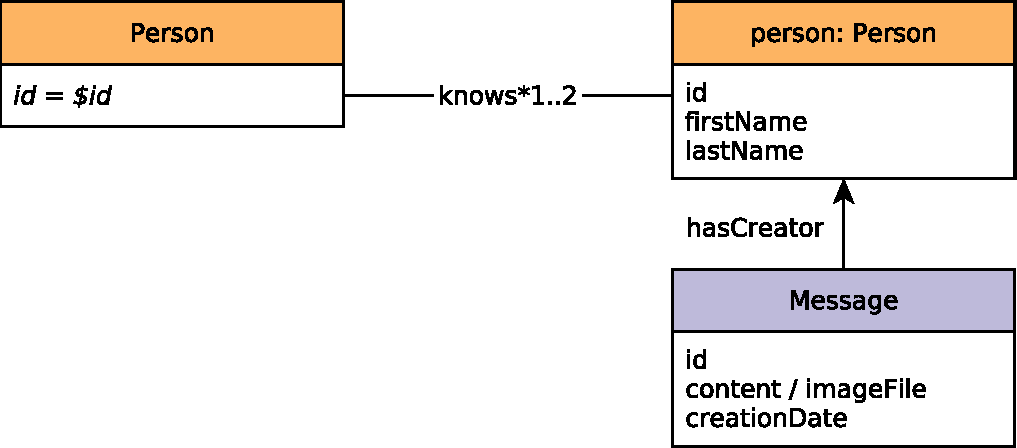
\includegraphics[scale=\patternscale,margin=0cm .2cm]{patterns/interactive-complex-read-09}} \\ \hline
%
	desc. & Given a start Person, find the (most recent) Messages created by that
Person's friends or friends of friends (excluding start Person). Only
consider the Messages created before a given date (excluding that date).
 \\ \hline
%
	
		params &
		\innerCardVSpace{\begin{tabularx}{\attributeCardWidth}{|>{\paramNumberCell}c|>{\varNameCell}M|>{\typeCell}m{\typeWidth}|Y|} \hline
		$\mathsf{1}$ & Person.id
 & ID
 &  \\ \hline
		$\mathsf{2}$ & date
 & Date
 &  \\ \hline
		\end{tabularx}}\innerCardVSpace \\ \hline
	
%
	
		result &
		\innerCardVSpace{\begin{tabularx}{\attributeCardWidth}{|>{\resultNumberCell}c|>{\varNameCell}M|>{\typeCell}m{\typeWidth}|>{\resultOriginCell}c|Y|} \hline
		$\mathsf{1}$ & Message-hasCreator-\textgreater{}Person.id & ID & R &
				\texttt{personId}
 \\ \hline
		$\mathsf{2}$ & Message-hasCreator-\textgreater{}Person.firstName & String & R &
				\texttt{personFirstName}
 \\ \hline
		$\mathsf{3}$ & Message-hasCreator-\textgreater{}Person.lastName & String & R &
				\texttt{personLastName}
 \\ \hline
		$\mathsf{4}$ & Message.id & ID & R &
				\texttt{commentOrPostId}
 \\ \hline
		$\mathsf{5}$ & Message.content or Post.imageFile & String & R &
				\texttt{commentOrPostContent}
 \\ \hline
		$\mathsf{6}$ & Message.creationDate & DateTime & R &
				\texttt{commentOrPostCreationDate}
 \\ \hline
		\end{tabularx}}\innerCardVSpace \\ \hline
	
%
	
		sort		&
		\innerCardVSpace{\begin{tabularx}{\attributeCardWidth}{|>{\sortNumberCell}c|>{\varNameCell}M|>{\directionCell}c|Y|} \hline
		$\mathsf{1}$ & Message.creationDate
 & $\desc
$ &  \\ \hline
		$\mathsf{2}$ & Message.id
 & $\asc
$ &  \\ \hline
		\end{tabularx}}\innerCardVSpace \\ \hline
	%
	limit & 20 \\ \hline
	%
	CPs &
	\multicolumn{1}{>{\raggedright}l|}{
		\chokePoint{1.1}, 
		\chokePoint{1.2}, 
		\chokePoint{2.2}, 
		\chokePoint{2.3}, 
		\chokePoint{3.2}, 
		\chokePoint{3.3}
		} \\ \hline
	%
	relevance &
		\footnotesize This query looks for paths of length two or three, starting from a given Person, moving to its friends and friends of
friends, and ending at their created Messages. This is one of the most complex queries, as the list of choke-points
indicates. This query is expected to touch variable amounts of data with entities of different characteristics, and
therefore, properly estimating cardinalities and selecting the proper operators will be crucial.
 \\ \hline%
\end{tabularx}
\queryCardVSpace

% change \emph back to the old one
\let\emph\oldemph
\renewcommand*{\arraystretch}{1.1}

\subsection*{Interactive / complex / 10}
\label{section:interactive-complex-read-10}

% change \emph{} to use sans-serif font
\let\oldemph\emph
\renewcommand{\emph}[1]{{\footnotesize \sf #1}}

\renewcommand{\currentQueryCard}{10}
\marginpar{
	\raggedleft
	\vspace{0.22ex}

	\queryRefCard{interactive-complex-read-01}{Interactive}{1}\\
	\queryRefCard{interactive-complex-read-02}{Interactive}{2}\\
	\queryRefCard{interactive-complex-read-03}{Interactive}{3}\\
	\queryRefCard{interactive-complex-read-04}{Interactive}{4}\\
	\queryRefCard{interactive-complex-read-05}{Interactive}{5}\\
	\queryRefCard{interactive-complex-read-06}{Interactive}{6}\\
	\queryRefCard{interactive-complex-read-07}{Interactive}{7}\\
	\queryRefCard{interactive-complex-read-08}{Interactive}{8}\\
	\queryRefCard{interactive-complex-read-09}{Interactive}{9}\\
	\queryRefCard{interactive-complex-read-10}{Interactive}{10}\\
	\queryRefCard{interactive-complex-read-11}{Interactive}{11}\\
	\queryRefCard{interactive-complex-read-12}{Interactive}{12}\\
	\queryRefCard{interactive-complex-read-13}{Interactive}{13}\\
	\queryRefCard{interactive-complex-read-14}{Interactive}{14}\\
}

\noindent\begin{tabularx}{\queryCardWidth}{|>{\queryPropertyCell}p{\queryPropertyCellWidth}|X|}
	\hline
	query & Interactive / complex / 10 \\ \hline
%
	title & Friend recommendation \\ \hline
%
	pattern & \multicolumn{1}{c|}{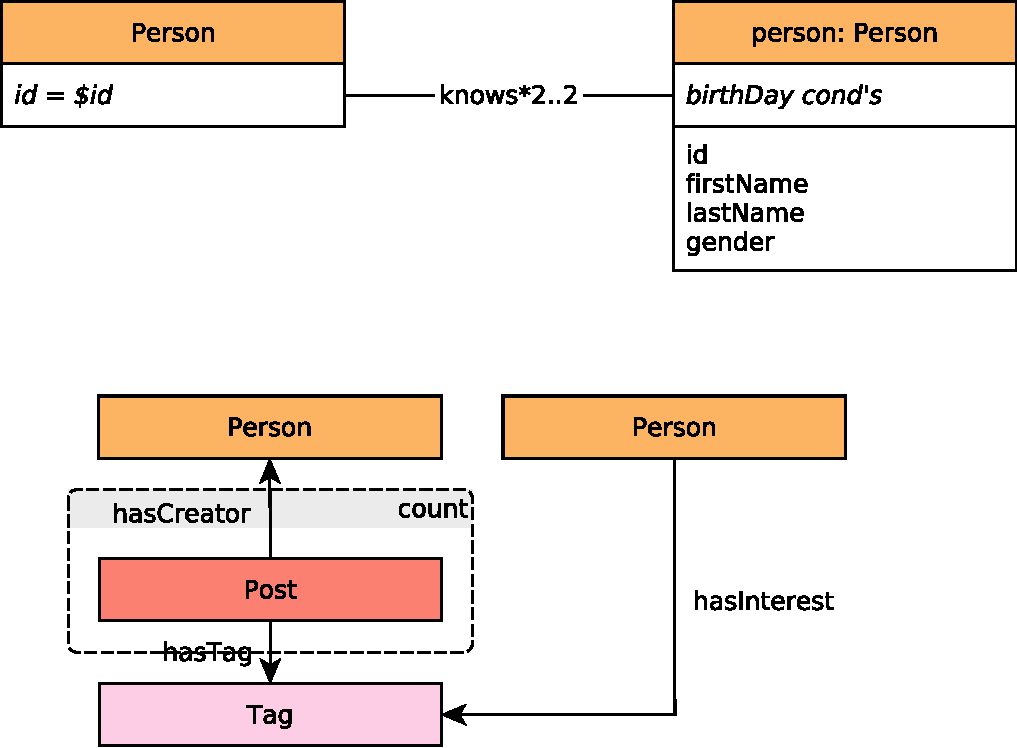
\includegraphics[scale=\patternscale,margin=0cm .2cm]{patterns/interactive-complex-read-10}} \\ \hline
%
	desc. & Given a start Person, find that Person's friends of friends (excluding
start Person, and immediate friends), who were born on or after the 21st
of a given month (in any year) and before the 22nd of the following
month. Calculate the similarity between each of these Persons and start
Person, where similarity for any Person is defined as follows:

\begin{itemize}
\tightlist
\item
  common = number of Posts created by that Person, such that the Post
  has a Tag that start Person is Interested in
\item
  uncommon = number of Posts created by that Person, such that the Post
  has no Tag that start Person is Interested in
\item
  similarity = common - uncommon
\end{itemize}
 \\ \hline
%
	
		params &
		\innerCardVSpace{\begin{tabularx}{\attributeCardWidth}{|>{\paramNumberCell}c|>{\varNameCell}M|>{\typeCell}m{\typeWidth}|Y|} \hline
		$\mathsf{1}$ & Person.id
 & ID
 &  \\ \hline
		$\mathsf{2}$ & month
 & 32-bit Integer
 & Between 1-12
 \\ \hline
		\end{tabularx}}\innerCardVSpace \\ \hline
	
%
	
		result &
		\innerCardVSpace{\begin{tabularx}{\attributeCardWidth}{|>{\resultNumberCell}c|>{\varNameCell}M|>{\typeCell}m{\typeWidth}|>{\resultOriginCell}c|Y|} \hline
		$\mathsf{1}$ & Person.id & ID & R &
				 \\ \hline
		$\mathsf{2}$ & Person.firstName & String & R &
				 \\ \hline
		$\mathsf{3}$ & Person.lastName & String & R &
				 \\ \hline
		$\mathsf{4}$ & similarity & 32-bit Integer & C &
				 \\ \hline
		$\mathsf{5}$ & Person.gender & String & R &
				 \\ \hline
		$\mathsf{6}$ & Person-isLocatedIn-\textgreater{}Place.name & String & R &
				 \\ \hline
		\end{tabularx}}\innerCardVSpace \\ \hline
	
%
	
		sort		&
		\innerCardVSpace{\begin{tabularx}{\attributeCardWidth}{|>{\sortNumberCell}c|>{\varNameCell}M|>{\directionCell}c|Y|} \hline
		$\mathsf{1}$ & similarity
 & $\desc
$ &  \\ \hline
		$\mathsf{2}$ & Person.id
 & $\asc
$ &  \\ \hline
		\end{tabularx}}\innerCardVSpace \\ \hline
	%
	limit & 10 \\ \hline
	%
	CPs &
	\multicolumn{1}{>{\raggedright}l|}{
		\chokePoint{2.3}, 
		\chokePoint{3.3}, 
		\chokePoint{4.1}, 
		\chokePoint{4.2}, 
		\chokePoint{5.1}, 
		\chokePoint{5.2}, 
		\chokePoint{6.1}, 
		\chokePoint{7.1}
		} \\ \hline
	%
	relevance &
		\small This query looks for paths of length two, starting from a Person and ending at the friends of their friends. It does
widely scattered graph traversal, and one expects no locality of in friends of friends, as these have been acquired
over a long time and have widely scattered identifiers. The join order is simple but one must see that the anti-join
for "not in my friends" is better with hash. Also the last pattern in the scalar sub-queries joining or anti-joining the
tags of the candidate's posts to interests of self should be by hash.
 \\ \hline%
\end{tabularx}
\queryCardVSpace

% change \emph back to the old one
\renewcommand{\emph}[1]{\oldemph{#1}}
\renewcommand*{\arraystretch}{1.1}

\subsection*{Interactive / complex / 11}
\label{section:interactive-complex-read-11}

% change \emph{} to use sans-serif font
\let\oldemph\emph
\renewcommand{\emph}[1]{{\footnotesize \sf #1}}

\renewcommand{\currentQueryCard}{11}
\marginpar{
	\raggedleft
	\vspace{0.22ex}

	\queryRefCard{interactive-complex-read-01}{IC}{1}\\
	\queryRefCard{interactive-complex-read-02}{IC}{2}\\
	\queryRefCard{interactive-complex-read-03}{IC}{3}\\
	\queryRefCard{interactive-complex-read-04}{IC}{4}\\
	\queryRefCard{interactive-complex-read-05}{IC}{5}\\
	\queryRefCard{interactive-complex-read-06}{IC}{6}\\
	\queryRefCard{interactive-complex-read-07}{IC}{7}\\
	\queryRefCard{interactive-complex-read-08}{IC}{8}\\
	\queryRefCard{interactive-complex-read-09}{IC}{9}\\
	\queryRefCard{interactive-complex-read-10}{IC}{10}\\
	\queryRefCard{interactive-complex-read-11}{IC}{11}\\
	\queryRefCard{interactive-complex-read-12}{IC}{12}\\
	\queryRefCard{interactive-complex-read-13}{IC}{13}\\
	\queryRefCard{interactive-complex-read-14}{IC}{14}\\
}


\noindent\begin{tabularx}{\queryCardWidth}{|>{\queryPropertyCell}p{\queryPropertyCellWidth}|X|}
	\hline
	query & Interactive / complex / 11 \\ \hline
%
	title & Job referral \\ \hline
%
	pattern & \multicolumn{1}{c|}{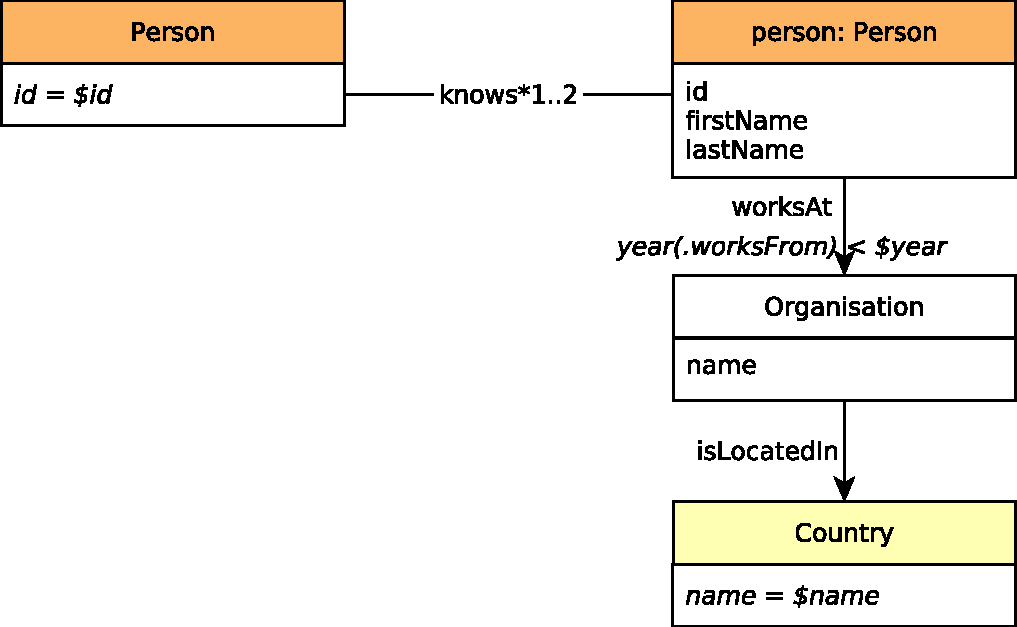
\includegraphics[scale=\patternscale,margin=0cm .2cm]{patterns/interactive-complex-read-11}} \\ \hline
%
	desc. & Given a start Person, find that Person's friends and friends of friends
(excluding start Person) who started Working in some Company in a given
Country, before a given date (year).
 \\ \hline
%
	
		params &
		\innerCardVSpace{\begin{tabularx}{\attributeCardWidth}{|>{\paramNumberCell}c|>{\varNameCell}M|>{\typeCell}m{\typeWidth}|Y|} \hline
		$\mathsf{1}$ & Person.id
 & ID
 & \texttt{Person}
 \\ \hline
		$\mathsf{2}$ & Country.name
 & String
 & \texttt{Country}
 \\ \hline
		$\mathsf{3}$ & year
 & 32-bit Integer
 & \texttt{Date0}
 \\ \hline
		\end{tabularx}}\innerCardVSpace \\ \hline
	
%
	
		result &
		\innerCardVSpace{\begin{tabularx}{\attributeCardWidth}{|>{\resultNumberCell}c|>{\varNameCell}M|>{\typeCell}m{\typeWidth}|>{\resultOriginCell}c|Y|} \hline
		$\mathsf{1}$ & Person.id & ID & R &
				\texttt{personId}
 \\ \hline
		$\mathsf{2}$ & Person.firstName & String & R &
				\texttt{personFirstName}
 \\ \hline
		$\mathsf{3}$ & Person.lastName & String & R &
				\texttt{personLastName}
 \\ \hline
		$\mathsf{4}$ & Person-worksAt-\textgreater{}Organisation.name & String & R &
				\texttt{organizationName}
 \\ \hline
		$\mathsf{5}$ & Person-worksAt-\textgreater{}.worksFrom & 32-bit Integer & R &
				\texttt{organizationWorkFromYear}
 \\ \hline
		\end{tabularx}}\innerCardVSpace \\ \hline
	
%
	
		sort		&
		\innerCardVSpace{\begin{tabularx}{\attributeCardWidth}{|>{\sortNumberCell}c|>{\varNameCell}M|>{\directionCell}c|Y|} \hline
		$\mathsf{1}$ & Person-worksAt-\textgreater{}.worksFrom
 & $\asc
$ &  \\ \hline
		$\mathsf{2}$ & Person.id
 & $\asc
$ &  \\ \hline
		$\mathsf{3}$ & Person-worksAt-\textgreater{}Organisation.name
 & $\desc
$ &  \\ \hline
		\end{tabularx}}\innerCardVSpace \\ \hline
	%
	limit & 10 \\ \hline
	%
	CPs &
	\multicolumn{1}{>{\raggedright}l|}{
		\chokePoint{1.3}, 
		\chokePoint{2.3}, 
		\chokePoint{2.4}, 
		\chokePoint{3.3}
		} \\ \hline
	%
	relevance &
		\footnotesize This query looks for paths of length two or three, starting from a Person, moving to friends or friends of friends,
and ending at a Company. In this query, there are selective joins and a top k order by that can be exploited for
optimizations.
 \\ \hline%
\end{tabularx}
\queryCardVSpace

% change \emph back to the old one
\let\emph\oldemph
\renewcommand*{\arraystretch}{1.1}

\subsection*{Interactive / complex / 12}
\label{section:interactive-complex-read-12}

% change \emph{} to use sans-serif font
\let\oldemph\emph
\renewcommand{\emph}[1]{{\footnotesize \sf #1}}

\renewcommand{\currentQueryCard}{12}
\marginpar{
	\raggedleft
	\vspace{0.22ex}

	\queryRefCard{interactive-complex-read-01}{Interactive}{1}\\
	\queryRefCard{interactive-complex-read-02}{Interactive}{2}\\
	\queryRefCard{interactive-complex-read-03}{Interactive}{3}\\
	\queryRefCard{interactive-complex-read-04}{Interactive}{4}\\
	\queryRefCard{interactive-complex-read-05}{Interactive}{5}\\
	\queryRefCard{interactive-complex-read-06}{Interactive}{6}\\
	\queryRefCard{interactive-complex-read-07}{Interactive}{7}\\
	\queryRefCard{interactive-complex-read-08}{Interactive}{8}\\
	\queryRefCard{interactive-complex-read-09}{Interactive}{9}\\
	\queryRefCard{interactive-complex-read-10}{Interactive}{10}\\
	\queryRefCard{interactive-complex-read-11}{Interactive}{11}\\
	\queryRefCard{interactive-complex-read-12}{Interactive}{12}\\
	\queryRefCard{interactive-complex-read-13}{Interactive}{13}\\
	\queryRefCard{interactive-complex-read-14}{Interactive}{14}\\
}

\noindent\begin{tabularx}{\queryCardWidth}{|>{\queryPropertyCell}p{\queryPropertyCellWidth}|X|}
	\hline
	query & Interactive / complex / 12 \\ \hline
%
	title & Expert search \\ \hline
%
	pattern & \hfill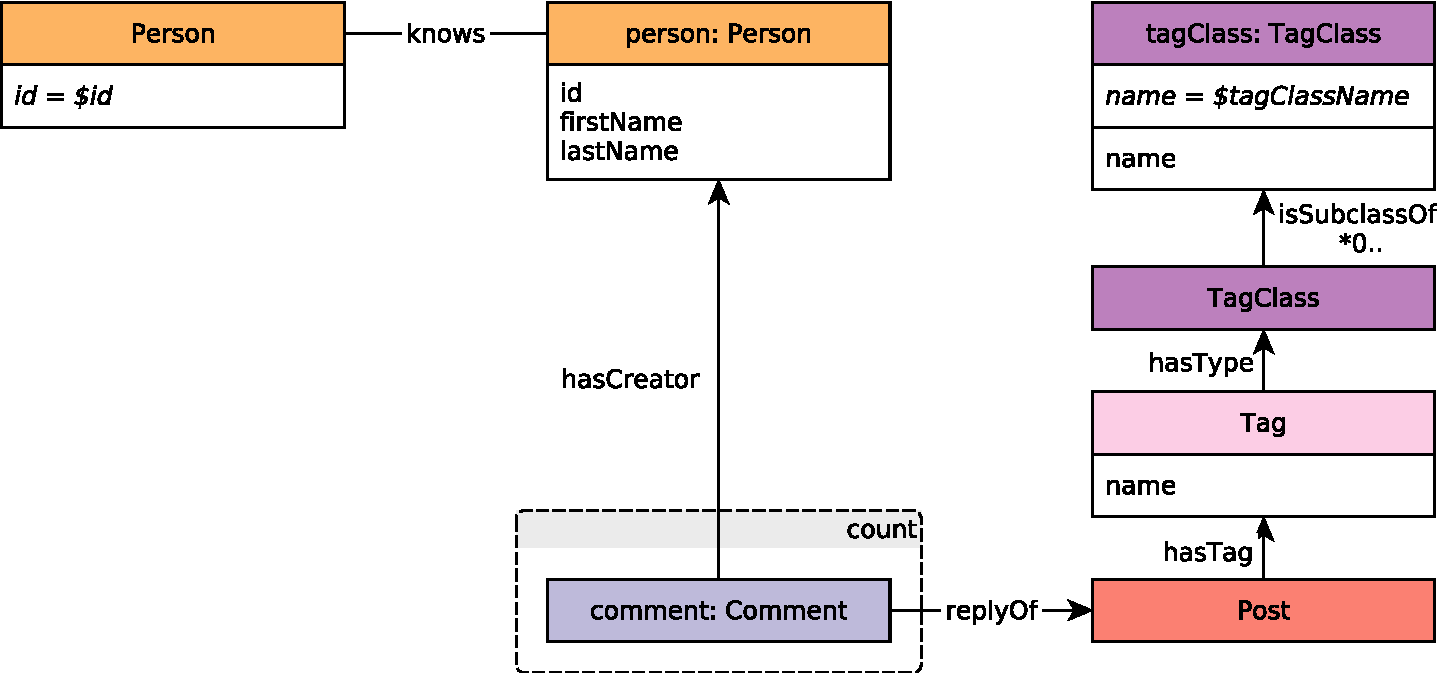
\includegraphics[scale=\patternscale,margin=0cm .2cm]{patterns/interactive-complex-read-12}\hfill \\ \hline
%
	desc. & Given a start Person, find the Comments that this Person's friends made
in reply to Posts, considering only those Comments that are immediate
(1-hop) replies to Posts, not the transitive (multi-hop) case. Only
consider Posts with a Tag in a given TagClass or in a descendent of that
TagClass. Count the number of these reply Comments, and collect the Tags
that were attached to the Posts they replied to, but only collect Tags
with the given TagClass or with a descendant of that TagClass Return
Persons with at least one reply, the reply count, and the collection of
Tags.
 \\ \hline
%
	
		params &
		\innerCardVSpace{\begin{tabularx}{\attributeCardWidth}{|>{\paramNumberCell}c|>{\varNameCell}M|>{\typeCell}m{\typeWidth}|Y|} \hline
		$\mathsf{1}$ & Person.id
 & ID
 &  \\ \hline
		$\mathsf{2}$ & TagClass.name
 & String
 &  \\ \hline
		\end{tabularx}}\innerCardVSpace \\ \hline
	
%
	
		result &
		\innerCardVSpace{\begin{tabularx}{\attributeCardWidth}{|>{\resultNumberCell}c|>{\varNameCell}M|>{\typeCell}m{\typeWidth}|>{\resultOriginCell}c|Y|} \hline
		$\mathsf{1}$ & Person.id & ID & R &
				 \\ \hline
		$\mathsf{2}$ & Person.firstName & String & R &
				 \\ \hline
		$\mathsf{3}$ & Person.lastName & String & R &
				 \\ \hline
		$\mathsf{4}$ & \{Tag.name\} & \{String\} & R &
				 \\ \hline
		$\mathsf{5}$ & count & 32-bit Integer & A &
				Number of reply Comments
 \\ \hline
		\end{tabularx}}\innerCardVSpace \\ \hline
	
%
	
		sort		&
		\innerCardVSpace{\begin{tabularx}{\attributeCardWidth}{|>{\sortNumberCell}c|>{\varNameCell}M|>{\directionCell}c|Y|} \hline
		$\mathsf{1}$ & count
 & $\desc
$ &  \\ \hline
		$\mathsf{2}$ & Person.id
 & $\asc
$ &  \\ \hline
		\end{tabularx}}\innerCardVSpace \\ \hline
	%
	limit & 20 \\ \hline
	%
	CPs &
	\multicolumn{1}{>{\raggedright}l|}{
		\chokePoint{1.5}, 
		\chokePoint{3.3}, 
		\chokePoint{7.2}, 
		\chokePoint{7.3}
		} \\ \hline
	%
	relevance &
		\small This query looks for paths of length three, starting at a Person, moving to its friends, the to their Comments and
ending at the Post the Comments are replying. The chain from original post to the reply is transitive. The traversal
may be initiated at either end, the system may note that this is a tree, hence leaf to root is always best. Additionally,
a hash table can be built from either end, e.g. from the friends of self, from the tags in the category, from the or
other.
 \\ \hline%
\end{tabularx}
\queryCardVSpace

% change \emph back to the old one
\renewcommand{\emph}[1]{\oldemph{#1}}
\renewcommand*{\arraystretch}{1.1}

\subsection*{Interactive / complex / 13}
\label{sec:interactive-complex-read-13}

\noindent\begin{tabularx}{\queryCardWidth}{|>{\queryPropertyCell}c|X|}
	\hline
	query & Interactive / complex / 13 \\ \hline
%
	title & Single shortest path \\ \hline
%
    pattern & \hfill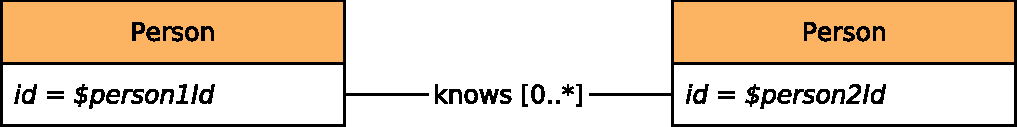
\includegraphics[scale=\patternscale,margin=0cm .2cm]{patterns/interactive-complex-read-13}\hfill\vadjust{} \\ \hline
%
	desc. & Given two Persons, find the shortest path between these two Persons in
the subgraph induced by the Knows relationships.

Return the length of this path:

\begin{itemize}
\tightlist
\item
  \(-1\) : no path found
\item
  \(0\): start person = end person
\item
  \(> 0\): regular case
\end{itemize}
 \\ \hline
%
	
%
    
        params &
        \innerCardVSpace{\begin{tabularx}{\attributeCardWidth}{|>{\paramNumberCell}c|>{\varNameCell}M|>{\typeCell}m{\typeWidth}|Y|} \hline
        \cellcolor{parameter} \color{white} \footnotesize $\mathsf{1}$ &person1.id& ID &  \\ \hline
        \cellcolor{parameter} \color{white} \footnotesize $\mathsf{2}$ &person2.id& ID &  \\ \hline
        \end{tabularx}}\innerCardVSpace \\ \hline
	
%
	
        result &
        \innerCardVSpace{\begin{tabularx}{\attributeCardWidth}{|>{\resultNumberCell}c|>{\varNameCell}M|>{\typeCell}m{\typeWidth}|>{\resultOriginCell}c|Y|} \hline
        $\mathsf{1}$ & length & 32-bit Integer &C&
                 \\ \hline
        \end{tabularx}}\innerCardVSpace \\ \hline
	
%
	%
	%
	CPs &
	\multicolumn{1}{>{\raggedright}l|}{
	    \chokePoint{3.3}, 
	    \chokePoint{7.2}, 
	    \chokePoint{7.3}
	    } \\ \hline
	%
    relevance &
        \small This query looks for a variable length path, starting at a given Person and finishing at an another given Person.
Proper cardinality estimation and search space prunning, will be crucial. This query also allows for possible parallel
implementations.
 \\ \hline%
\end{tabularx}
\queryCardVSpace
\renewcommand*{\arraystretch}{1.1}

\subsection*{Interactive / complex / 14}
\label{sec:interactive-complex-read-14}

\noindent\begin{tabularx}{\queryCardWidth}{|>{\queryPropertyCell}p{\queryPropertyCellWidth}|X|}
	\hline
	query & Interactive / complex / 14 \\ \hline
%
	title & Weighted/unweighted paths
 \\ \hline
%
	pattern & \hfill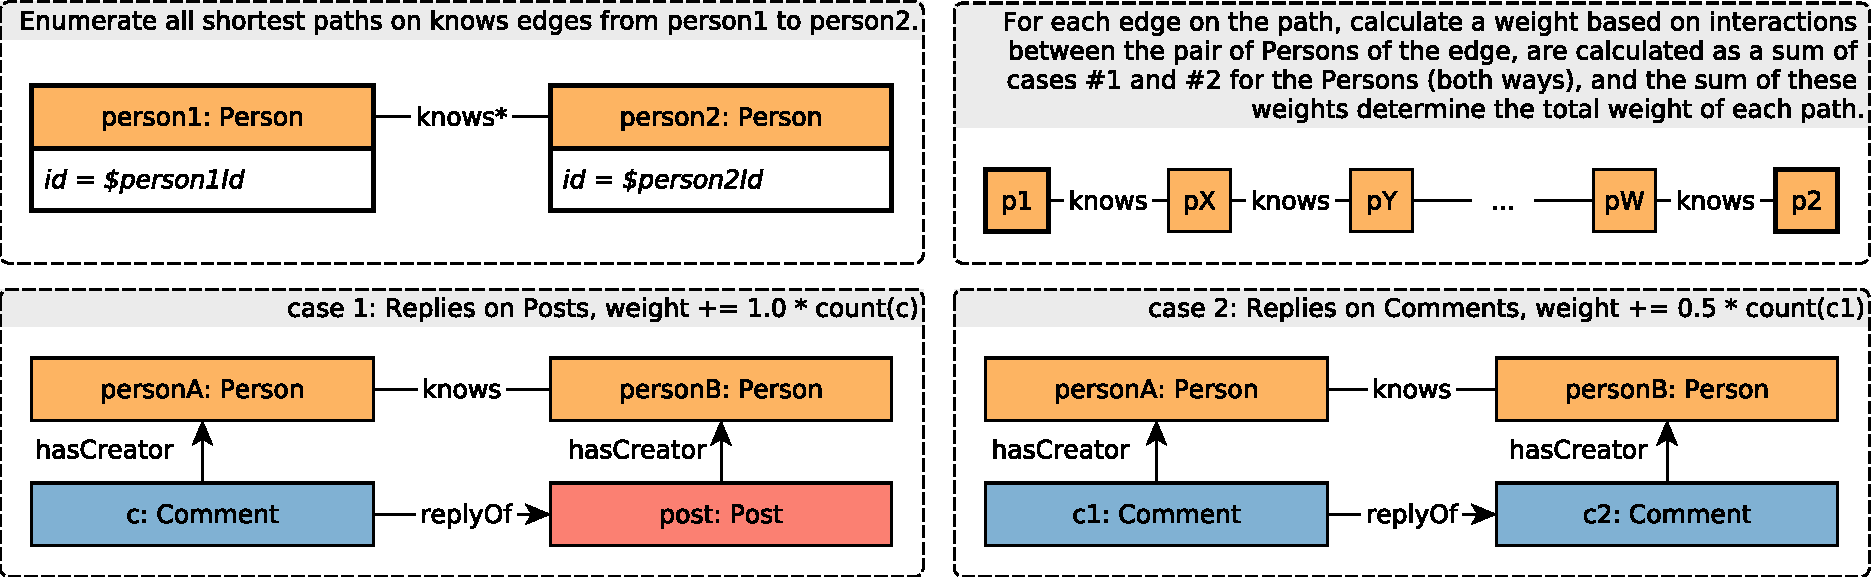
\includegraphics[scale=\patternscale,margin=0cm .2cm]{patterns/interactive-complex-read-14}\hfill\vadjust{} \\ \hline
%
	desc. & Given two Persons, find all (unweighted) shortest paths between these
two Persons, in the subgraph induced by the Knows relationship. Then,
for each path calculate a weight. The nodes in the path are Persons, and
the weight of a path is the sum of weights between every pair of
consecutive Person nodes in the path. The weight for a pair of Persons
is calculated such that every reply (by one of the Persons) to a Post
(by the other Person) contributes 1.0, and every reply (by ones of the
Persons) to a Comment (by the other Person) contributes 0.5. Return all
the paths with shortest length, and their weights. Do not return any
rows if there is now path between the two Persons.
 \\ \hline
%
	
%
	
		params &
		\innerCardVSpace{\begin{tabularx}{\attributeCardWidth}{|>{\paramNumberCell}c|>{\varNameCell}M|>{\typeCell}m{\typeWidth}|Y|} \hline
		$\mathsf{1}$ & person1.id
 & ID
 &  \\ \hline
		$\mathsf{2}$ & person2.id
 & ID
 &  \\ \hline
		\end{tabularx}}\innerCardVSpace \\ \hline
	
%
	
		result &
		\innerCardVSpace{\begin{tabularx}{\attributeCardWidth}{|>{\resultNumberCell}c|>{\varNameCell}M|>{\typeCell}m{\typeWidth}|>{\resultOriginCell}c|Y|} \hline
		$\mathsf{1}$ & {[}Person.id{]}
 & {[}ID{]}
 & R &
				Identifiers representing an ordered sequence of the Persons in the path
 \\ \hline
		$\mathsf{2}$ & weight
 & 64-bit Float
 & R &
				 \\ \hline
		\end{tabularx}}\innerCardVSpace \\ \hline
	
%
	
		sort		&
		\innerCardVSpace{\begin{tabular}{|>{\sortNumberCell}c|>{\varNameCell}l|>{\directionCell}c|} \hline
		$\mathsf{1}$ & weight
 & $\desc
$ \\ \hline
		\end{tabular}}\innerCardVSpace \\ \hline
	%
	%
	CPs &
	\multicolumn{1}{>{\raggedright}l|}{
		\chokePoint{3.3}, 
		\chokePoint{7.2}, 
		\chokePoint{7.3}
		} \\ \hline
	%
	relevance &
		\small This query looks for a variable length path, starting at a given Person and finishing at an another given Person. This
is a more complex query as not only requires computing the path length, but returning it and computing a weight.
To compute this weight one must look for smaller sub-queries with paths of length three, formed by the two Persons
at each step, a Post and a Comment.
 \\ \hline%
\end{tabularx}
\queryCardVSpace

% reset counter to make sure the last query card isn't stuck in highlighted mode
\renewcommand{\currentQueryCard}{0}


\renewcommand*{\arraystretch}{1.1}

\noindent\begin{tabularx}{17cm}{|p{1.95cm}|X|}
	\hline
	number      & 1                                                          \\ \hline
%
	title       & Friends with certain name                                                           \\ \hline
	\multicolumn{2}{|c|}{ 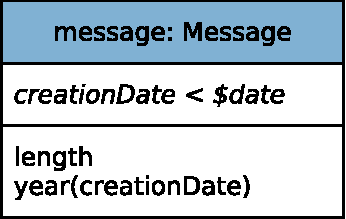
\includegraphics[scale=\patternscale,margin=0cm .2cm]{patterns/q01}} \\ \hline
	description & Given a start Person, find Persons with a given first name that the
start Person is connected to (excluding start Person) by at most 3 steps
via Knows relationships. Return Persons, including summaries of the
Persons workplaces and places of study.
 \\ \hline
	
%
	parameters  &
	\vspace{1.1ex}{\begin{tabularx}{14.2cm}{|c|l|m{2cm}|Y|} \hline
	\cellcolor{black!70} \color{white} $\mathsf{1}$ & \varname{Person.id} & \cellcolor{gray!20} \vartype{ID} &  \\\hline
	\cellcolor{black!70} \color{white} $\mathsf{2}$ & \varname{Person.firstName} & \cellcolor{gray!20} \vartype{String} &  \\
	\end{tabularx}} \\ \hline
%
	result      &
	\vspace{1.1ex}{\begin{tabularx}{14.2cm}{|c|l|m{2cm}|Y|} \hline
	\cellcolor{black!70} \color{white} $\mathsf{1}$ & \varname{Person.id} & \cellcolor{gray!20} \vartype{ID} &  \\\hline
	\cellcolor{black!70} \color{white} $\mathsf{2}$ & \varname{Person.lastName} & \cellcolor{gray!20} \vartype{String} &  \\\hline
	\cellcolor{black!70} \color{white} $\mathsf{3}$ & \varname{Person.birthday} & \cellcolor{gray!20} \vartype{Date} &  \\\hline
	\cellcolor{black!70} \color{white} $\mathsf{4}$ & \varname{Person.creationDate} & \cellcolor{gray!20} \vartype{DateTime} &  \\\hline
	\cellcolor{black!70} \color{white} $\mathsf{5}$ & \varname{Person.gender} & \cellcolor{gray!20} \vartype{String} &  \\\hline
	\cellcolor{black!70} \color{white} $\mathsf{6}$ & \varname{Person.browserUsed} & \cellcolor{gray!20} \vartype{String} &  \\\hline
	\cellcolor{black!70} \color{white} $\mathsf{7}$ & \varname{Person.locationIP} & \cellcolor{gray!20} \vartype{String} &  \\\hline
	\cellcolor{black!70} \color{white} $\mathsf{8}$ & \varname{\{Person.emails\}} & \cellcolor{gray!20} \vartype{\{String\}} &  \\\hline
	\cellcolor{black!70} \color{white} $\mathsf{9}$ & \varname{\{Person.language\}} & \cellcolor{gray!20} \vartype{\{String\}} &  \\\hline
	\cellcolor{black!70} \color{white} $\mathsf{10}$ & \varname{Person-isLocatedIn->Place.name} & \cellcolor{gray!20} \vartype{String} &  \\\hline
	\cellcolor{black!70} \color{white} $\mathsf{11}$ & \varname{\{Person-studyAt->University.name, Person-studyAt->.classYear, Person-studyAt->University-isLocatedIn->City.name\}} & \cellcolor{gray!20} \vartype{\{<String, 32-bit Integer, String>\}} &  \\\hline
	\cellcolor{black!70} \color{white} $\mathsf{12}$ & \varname{\{Person-workAt->Company.name, Person-workAt->.workFrom, Person-workAt->Company-isLocatedIn->Country.name\}} & \cellcolor{gray!20} \vartype{\{<String, 32-bit Integer, String>\}} &  \\
	\end{tabularx}} \\ \hline
	%
	sort        &
	\vspace{1.1ex}{\begin{tabular}{|c|l|c|} \hline
	\cellcolor{black!70} \color{white} $\mathsf{1}$ & \varname{distance from person} & \cellcolor{gray!20} $\asc$ \\\hline
	\cellcolor{black!70} \color{white} $\mathsf{2}$ & \varname{Person.lastName} & \cellcolor{gray!20} $\asc$ \\\hline
	\cellcolor{black!70} \color{white} $\mathsf{3}$ & \varname{Person.id} & \cellcolor{gray!20} $\asc$ \\
	\end{tabular}} \\ \hline
	%
	limit       & 20 \\ \hline
	%
	choke points &
	\multicolumn{1}{>{\raggedright}X|}{
		}\\ \hline
\end{tabularx}
\clearpage
\renewcommand*{\arraystretch}{1.1}

\noindent\begin{tabularx}{17cm}{|p{1.95cm}|X|}
	\hline
	workload    & Interactive \\ \hline
%
	query       & 2 \\ \hline
%
	title       & Recent posts and comments by your friends \\ \hline
%
    pattern     & \hfill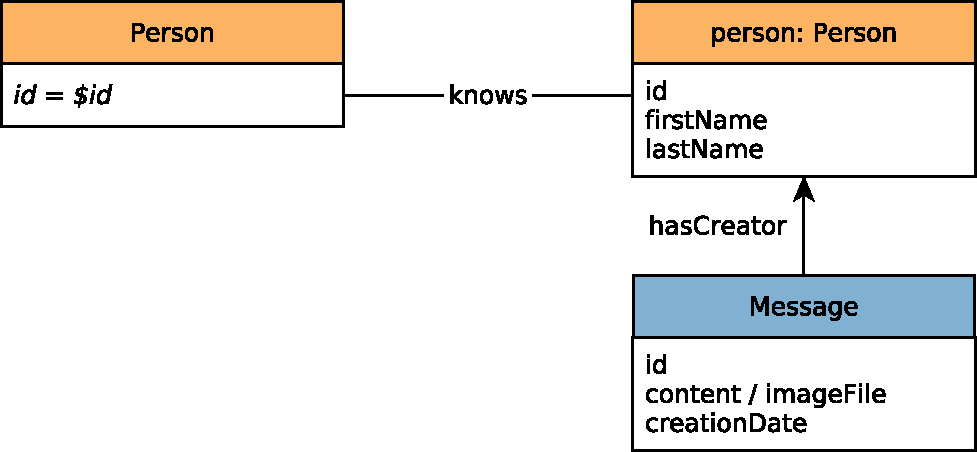
\includegraphics[scale=\patternscale,margin=0cm .2cm]{patterns/interactive02}\hfill\vadjust{} \\ \hline
%
	description & Given a start Person, find (most recent) Messages from all of that
Person's friends, that were created before (and including) a given date.
 \\ \hline
	
%
	parameters  &
	\vspace{1.1ex}{\begin{tabularx}{14.2cm}{|c|M|m{2cm}|Y|} \hline
	\cellcolor{black!70} \color{white} $\mathsf{1}$ & \varname{Person.id} & \cellcolor{gray!20} \vartype{ID} &  \\ \hline
	\cellcolor{black!70} \color{white} $\mathsf{2}$ & \varname{date} & \cellcolor{gray!20} \vartype{DateTime} &  \\ \hline
	\end{tabularx}}\vspace{1.1ex} \\ \hline
%
	result      &
	\vspace{1.1ex}{\begin{tabularx}{14.2cm}{|c|M|m{2cm}|Y|} \hline
	\cellcolor{black!70} \color{white} $\mathsf{1}$ & \varname{Message-hasCreator->Person.id} & \cellcolor{gray!20} \vartype{ID} &  \\ \hline
	\cellcolor{black!70} \color{white} $\mathsf{2}$ & \varname{Message-hasCreator->Person.firstName} & \cellcolor{gray!20} \vartype{String} &  \\ \hline
	\cellcolor{black!70} \color{white} $\mathsf{3}$ & \varname{Message-hasCreator->Person.lastName} & \cellcolor{gray!20} \vartype{String} &  \\ \hline
	\cellcolor{black!70} \color{white} $\mathsf{4}$ & \varname{Message.id} & \cellcolor{gray!20} \vartype{ID} &  \\ \hline
	\cellcolor{black!70} \color{white} $\mathsf{5}$ & \varname{Message.content or Post.imageFile} & \cellcolor{gray!20} \vartype{String} &  \\ \hline
	\cellcolor{black!70} \color{white} $\mathsf{6}$ & \varname{Message.creationDate} & \cellcolor{gray!20} \vartype{DateTime} &  \\ \hline
	\end{tabularx}}\vspace{1.1ex} \\ \hline
	%
	sort        &
	\vspace{1.1ex}{\begin{tabular}{|c|l|c|} \hline
	\cellcolor{black!70} \color{white} $\mathsf{1}$ & \varname{Message.creationDate} & \cellcolor{gray!20} $\desc$ \\ \hline
	\cellcolor{black!70} \color{white} $\mathsf{2}$ & \varname{Message.id} & \cellcolor{gray!20} $\asc$ \\ \hline
	\end{tabular}}\vspace{1.1ex} \\ \hline
	%
	limit       & 20 \\ \hline
	%
	choke points &
	\multicolumn{1}{>{\raggedright}X|}{
		}\\ \hline
\end{tabularx}
\clearpage
\renewcommand*{\arraystretch}{1.1}

\noindent\begin{tabularx}{17cm}{|p{1.95cm}|X|}
	\hline
	workload    & Interactive \\ \hline
%
	query       & 3 \\ \hline
%
	title       & Friends and friends of friends that have been to countries X and Y \\ \hline
%
    pattern     & \hfill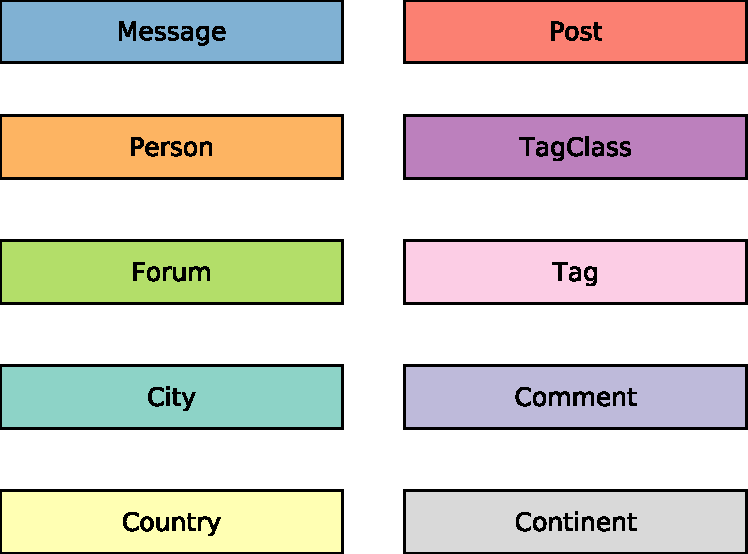
\includegraphics[scale=\patternscale,margin=0cm .2cm]{patterns/interactive03}\hfill\vadjust{} \\ \hline
%
	description & Given a start Person, find Persons that are their friends and friends of
friends (excluding start Person) that have made Posts/Comments in both
of the given Countries, X and Y, within a given period. Only Persons
that are foreign to Countries X and Y are considered, that is Persons
whose Location is not Country X or Country Y.
 \\ \hline
	
%
	parameters  &
	\vspace{1.1ex}{\begin{tabularx}{14.2cm}{|c|M|m{2cm}|Y|} \hline
	\cellcolor{black!70} \color{white} $\mathsf{1}$ & \varname{Person.id} & \cellcolor{gray!20} \vartype{ID} &  \\ \hline
	\cellcolor{black!70} \color{white} $\mathsf{2}$ & \varname{CountryX.name} & \cellcolor{gray!20} \vartype{String} &  \\ \hline
	\cellcolor{black!70} \color{white} $\mathsf{3}$ & \varname{CountryY.name} & \cellcolor{gray!20} \vartype{String} &  \\ \hline
	\cellcolor{black!70} \color{white} $\mathsf{4}$ & \varname{startDate} & \cellcolor{gray!20} \vartype{Date} & beginning of requested period \\ \hline
	\cellcolor{black!70} \color{white} $\mathsf{5}$ & \varname{duration} & \cellcolor{gray!20} \vartype{32-bit Integer} & duration of requested period, in days the interval [startDate, startDate + Duration) is closed-open \\ \hline
	\end{tabularx}}\vspace{1.1ex} \\ \hline
%
	result      &
	\vspace{1.1ex}{\begin{tabularx}{14.2cm}{|c|M|m{2cm}|Y|} \hline
	\cellcolor{black!70} \color{white} $\mathsf{1}$ & \varname{Person.id} & \cellcolor{gray!20} \vartype{ID} &  \\ \hline
	\cellcolor{black!70} \color{white} $\mathsf{2}$ & \varname{Person.firstName} & \cellcolor{gray!20} \vartype{String} &  \\ \hline
	\cellcolor{black!70} \color{white} $\mathsf{3}$ & \varname{Person.lastName} & \cellcolor{gray!20} \vartype{String} &  \\ \hline
	\cellcolor{black!70} \color{white} $\mathsf{4}$ & \varname{countX} & \cellcolor{gray!20} \vartype{32-bit Integer} & number of Messages from Country X made by Person within the given time \\ \hline
	\cellcolor{black!70} \color{white} $\mathsf{5}$ & \varname{countY} & \cellcolor{gray!20} \vartype{32-bit Integer} & number of Messages from Country Y made by Person within the given time \\ \hline
	\cellcolor{black!70} \color{white} $\mathsf{6}$ & \varname{count} & \cellcolor{gray!20} \vartype{32-bit Integer} & countX + countY \\ \hline
	\end{tabularx}}\vspace{1.1ex} \\ \hline
	%
	sort        &
	\vspace{1.1ex}{\begin{tabular}{|c|l|c|} \hline
	\cellcolor{black!70} \color{white} $\mathsf{1}$ & \varname{countX} & \cellcolor{gray!20} $\desc$ \\ \hline
	\cellcolor{black!70} \color{white} $\mathsf{2}$ & \varname{Person.id} & \cellcolor{gray!20} $\asc$ \\ \hline
	\end{tabular}}\vspace{1.1ex} \\ \hline
	%
	limit       & 20 \\ \hline
	%
	choke points &
	\multicolumn{1}{>{\raggedright}X|}{
		}\\ \hline
\end{tabularx}
\clearpage
\renewcommand*{\arraystretch}{1.1}

\noindent\begin{tabularx}{17cm}{|p{1.95cm}|X|}
	\hline
	workload    & Interactive \\ \hline
%
	query       & 4 \\ \hline
%
	title       & New topics \\ \hline
	\multicolumn{2}{|c|}{ 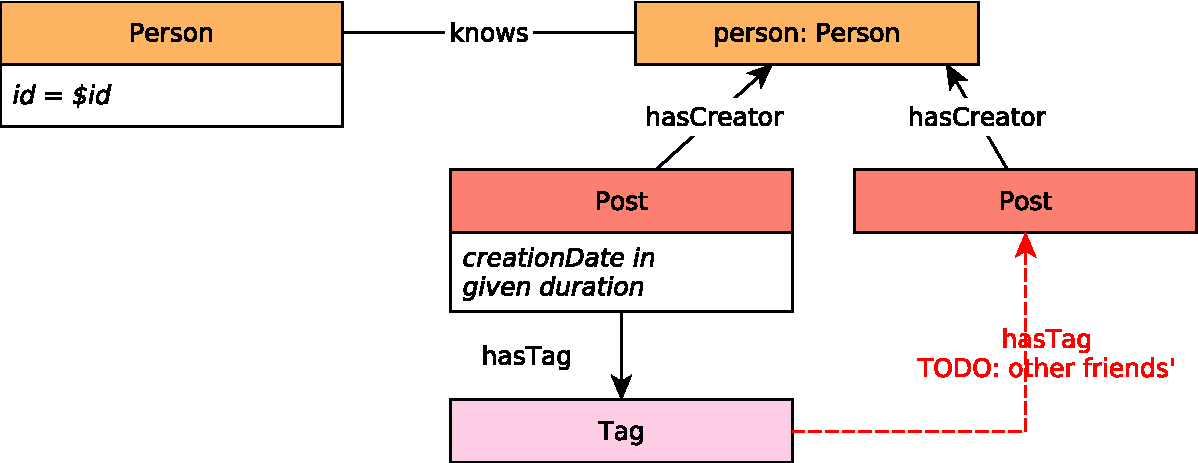
\includegraphics[scale=\patternscale,margin=0cm .2cm]{patterns/interactive04}} \\ \hline
	description & Given a start Person, find Tags that are attached to Posts that were
created by that Person's friends. Only include Tags that were attached
to friends' Posts created within a given time interval, and that were
never attached to friends' Posts created before this interval.
 \\ \hline
	
%
	parameters  &
	\vspace{1.1ex}{\begin{tabularx}{14.2cm}{|c|M|m{2cm}|Y|} \hline
	\cellcolor{black!70} \color{white} $\mathsf{1}$ & \varname{Person.id} & \cellcolor{gray!20} \vartype{ID} &  \\ \hline
	\cellcolor{black!70} \color{white} $\mathsf{2}$ & \varname{startDate} & \cellcolor{gray!20} \vartype{Date} &  \\ \hline
	\cellcolor{black!70} \color{white} $\mathsf{3}$ & \varname{duration} & \cellcolor{gray!20} \vartype{32-bit Integer} & duration of requested period, in days the interval [startDate, startDate + Duration) is closed-open \\ \hline
	\end{tabularx}}\vspace{1.1ex} \\ \hline
%
	result      &
	\vspace{1.1ex}{\begin{tabularx}{14.2cm}{|c|M|m{2cm}|Y|} \hline
	\cellcolor{black!70} \color{white} $\mathsf{1}$ & \varname{Tag.name} & \cellcolor{gray!20} \vartype{String} &  \\ \hline
	\cellcolor{black!70} \color{white} $\mathsf{2}$ & \varname{count} & \cellcolor{gray!20} \vartype{32-bit Integer} & number of Posts made within the given time interval that have this Tag \\ \hline
	\end{tabularx}}\vspace{1.1ex} \\ \hline
	%
	sort        &
	\vspace{1.1ex}{\begin{tabular}{|c|l|c|} \hline
	\cellcolor{black!70} \color{white} $\mathsf{1}$ & \varname{count} & \cellcolor{gray!20} $\desc$ \\ \hline
	\cellcolor{black!70} \color{white} $\mathsf{2}$ & \varname{Tag.name} & \cellcolor{gray!20} $\asc$ \\ \hline
	\end{tabular}}\vspace{1.1ex} \\ \hline
	%
	limit       & 10 \\ \hline
	%
	choke points &
	\multicolumn{1}{>{\raggedright}X|}{
		}\\ \hline
\end{tabularx}
\clearpage
\renewcommand*{\arraystretch}{1.1}

\noindent\begin{tabularx}{17cm}{|p{1.95cm}|X|}
	\hline
	workload    & Interactive \\ \hline
%
	query       & 5 \\ \hline
%
	title       & New groups \\ \hline
	\multicolumn{2}{|c|}{ 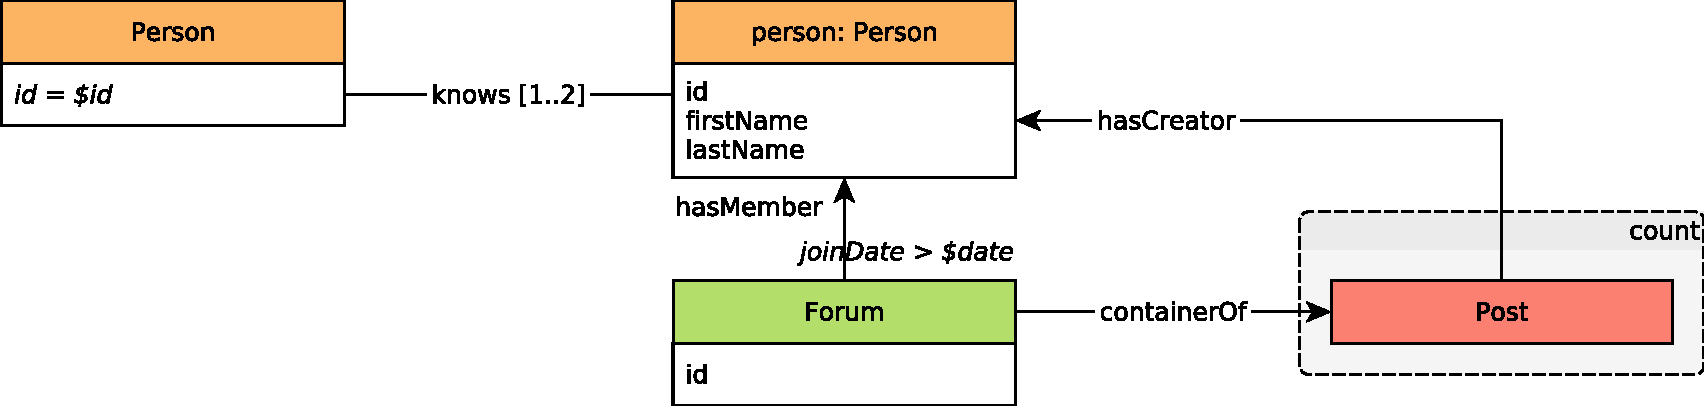
\includegraphics[scale=\patternscale,margin=0cm .2cm]{patterns/interactive05}} \\ \hline
	description & Given a start Person, find the Forums which that Person's friends and
friends of friends (excluding start Person) became Members of after a
given date. For each forum find the number of Posts that were created by
any of these Persons. For each Forum and consider only those Persons
which joined that particular Forum after the given date.
 \\ \hline
	
%
	parameters  &
	\vspace{1.1ex}{\begin{tabularx}{14.38cm}{|c|M|m{2cm}|Y} \hline
	\cellcolor{black!70} \color{white} $\mathsf{1}$ & \varname{Person.id} & \cellcolor{gray!20} \vartype{ID} &  \\\hline
	\cellcolor{black!70} \color{white} $\mathsf{2}$ & \varname{date} & \cellcolor{gray!20} \vartype{Date} &  \\
	\end{tabularx}} \\ \hline
%
	result      &
	\vspace{1.1ex}{\begin{tabularx}{14.38cm}{|c|M|m{2cm}|Y} \hline
	\cellcolor{black!70} \color{white} $\mathsf{1}$ & \varname{Forum.title} & \cellcolor{gray!20} \vartype{String} &  \\\hline
	\cellcolor{black!70} \color{white} $\mathsf{2}$ & \varname{count} & \cellcolor{gray!20} \vartype{32-bit Integer} & number of Posts made in Forum that were created by friends \\
	\end{tabularx}} \\ \hline
	%
	sort        &
	\vspace{1.1ex}{\begin{tabular}{|c|l|c|} \hline
	\cellcolor{black!70} \color{white} $\mathsf{1}$ & \varname{count} & \cellcolor{gray!20} $\desc$ \\\hline
	\cellcolor{black!70} \color{white} $\mathsf{2}$ & \varname{Forum.id} & \cellcolor{gray!20} $\asc$ \\
	\end{tabular}} \\ \hline
	%
	limit       & 20 \\ \hline
	%
	choke points &
	\multicolumn{1}{>{\raggedright}X|}{
		}\\ \hline
\end{tabularx}
\clearpage
\renewcommand*{\arraystretch}{1.1}

\noindent\begin{tabularx}{17cm}{|p{1.95cm}|X|}
	\hline
	workload    & interactive \\ \hline
%
	query       & 6 \\ \hline
%
	title       & Tag co-occurrence \\ \hline
	\multicolumn{2}{|c|}{ 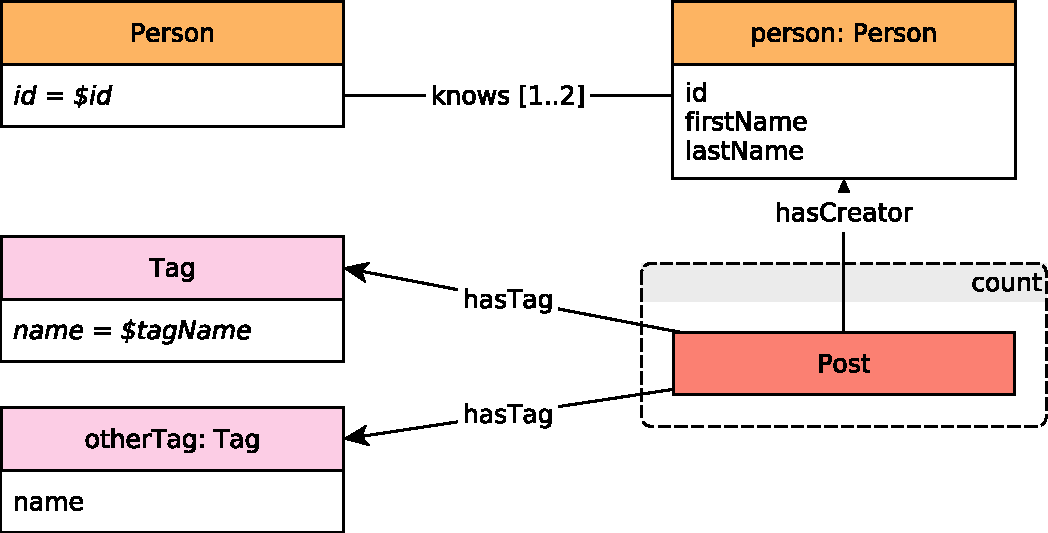
\includegraphics[scale=\patternscale,margin=0cm .2cm]{patterns/interactive06}} \\ \hline
	description & Given a start Person and some Tag, find the other Tags that occur
together with this Tag on Posts that were created by start Person's
friends and friends of friends (excluding start Person). Return For each
Tag, find the count of Posts that were created by these Persons, which
contain both this Tag and the given Tag.
 \\ \hline
	
%
	parameters  &
	\vspace{1.1ex}{\begin{tabularx}{14.38cm}{|c|M|m{2cm}|Y} \hline
	\cellcolor{black!70} \color{white} $\mathsf{1}$ & \varname{Person.id} & \cellcolor{gray!20} \vartype{ID} &  \\\hline
	\cellcolor{black!70} \color{white} $\mathsf{2}$ & \varname{Tag.name} & \cellcolor{gray!20} \vartype{String} &  \\
	\end{tabularx}} \\ \hline
%
	result      &
	\vspace{1.1ex}{\begin{tabularx}{14.38cm}{|c|M|m{2cm}|Y} \hline
	\cellcolor{black!70} \color{white} $\mathsf{1}$ & \varname{Tag.name} & \cellcolor{gray!20} \vartype{String} &  \\\hline
	\cellcolor{black!70} \color{white} $\mathsf{2}$ & \varname{count} & \cellcolor{gray!20} \vartype{32-bit Integer} & number of Posts that were created by friends and friends of friends, which contain this Tag \\
	\end{tabularx}} \\ \hline
	%
	sort        &
	\vspace{1.1ex}{\begin{tabular}{|c|l|c|} \hline
	\cellcolor{black!70} \color{white} $\mathsf{1}$ & \varname{count} & \cellcolor{gray!20} $\desc$ \\\hline
	\cellcolor{black!70} \color{white} $\mathsf{2}$ & \varname{Tag.name} & \cellcolor{gray!20} $\asc$ \\
	\end{tabular}} \\ \hline
	%
	limit       & 10 \\ \hline
	%
	choke points &
	\multicolumn{1}{>{\raggedright}X|}{
		}\\ \hline
\end{tabularx}
\clearpage
\renewcommand*{\arraystretch}{1.1}

\noindent\begin{tabularx}{17cm}{|p{1.95cm}|X|}
	\hline
	workload    & interactive \\ \hline
%
	query       & 7 \\ \hline
%
	title       & Recent likers \\ \hline
	\multicolumn{2}{|c|}{ 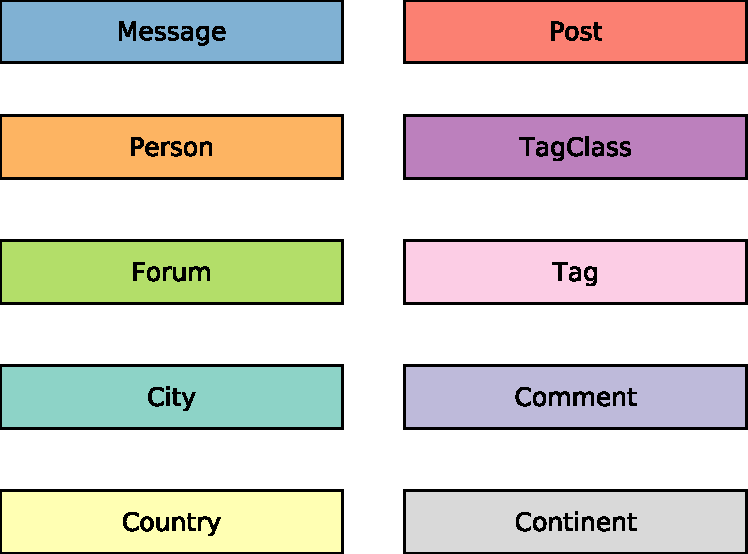
\includegraphics[scale=\patternscale,margin=0cm .2cm]{patterns/interactive07}} \\ \hline
	description & Given a start Person, find (most recent) Likes on any of start Person's
Messages. Find Persons that Liked any of start Person's Messages, the
Messages they liked most recently, creation date of that Like, and the
latency (in minutes) between creation of Messages and Like.
Additionally, for each Person found return a flag indicating whether the
liker is a friend of start Person. In the case that a Person Liked
multiple Messages at the same time, return the Message with lowest
identifier.
 \\ \hline
	
%
	parameters  &
	\vspace{1.1ex}{\begin{tabularx}{14.38cm}{|c|M|m{2cm}|Y} \hline
	\cellcolor{black!70} \color{white} $\mathsf{1}$ & \varname{Person.id} & \cellcolor{gray!20} \vartype{64-bit Integer} &  \\
	\end{tabularx}} \\ \hline
%
	result      &
	\vspace{1.1ex}{\begin{tabularx}{14.38cm}{|c|M|m{2cm}|Y} \hline
	\cellcolor{black!70} \color{white} $\mathsf{1}$ & \varname{Person.id} & \cellcolor{gray!20} \vartype{ID} &  \\\hline
	\cellcolor{black!70} \color{white} $\mathsf{2}$ & \varname{Person.firstName} & \cellcolor{gray!20} \vartype{String} &  \\\hline
	\cellcolor{black!70} \color{white} $\mathsf{3}$ & \varname{Person.lastName} & \cellcolor{gray!20} \vartype{String} &  \\\hline
	\cellcolor{black!70} \color{white} $\mathsf{4}$ & \varname{Like.creationDate} & \cellcolor{gray!20} \vartype{DateTime} &  \\\hline
	\cellcolor{black!70} \color{white} $\mathsf{5}$ & \varname{Message.id} & \cellcolor{gray!20} \vartype{ID} &  \\\hline
	\cellcolor{black!70} \color{white} $\mathsf{6}$ & \varname{Message.content or Post.imageFile} & \cellcolor{gray!20} \vartype{String} &  \\\hline
	\cellcolor{black!70} \color{white} $\mathsf{7}$ & \varname{latency} & \cellcolor{gray!20} \vartype{32-bit Integer} & duration between creation of\par Message and Like, in minutes \\\hline
	\cellcolor{black!70} \color{white} $\mathsf{8}$ & \varname{isNew} & \cellcolor{gray!20} \vartype{Boolean} & false if liker Person is friend of\par start Person, true otherwise \\
	\end{tabularx}} \\ \hline
	%
	sort        &
	\vspace{1.1ex}{\begin{tabular}{|c|l|c|} \hline
	\cellcolor{black!70} \color{white} $\mathsf{1}$ & \varname{Like.creationDate} & \cellcolor{gray!20} $\desc$ \\\hline
	\cellcolor{black!70} \color{white} $\mathsf{2}$ & \varname{Person.id} & \cellcolor{gray!20} $\asc$ \\
	\end{tabular}} \\ \hline
	%
	limit       & 20 \\ \hline
	%
	choke points &
	\multicolumn{1}{>{\raggedright}X|}{
		}\\ \hline
\end{tabularx}
\clearpage
\renewcommand*{\arraystretch}{1.1}

\noindent\begin{tabularx}{17cm}{|p{1.95cm}|X|}
	\hline
	workload    & Interactive \\ \hline
%
	query       & 8 \\ \hline
%
	title       & Recent replies \\ \hline
	\multicolumn{2}{|c|}{ 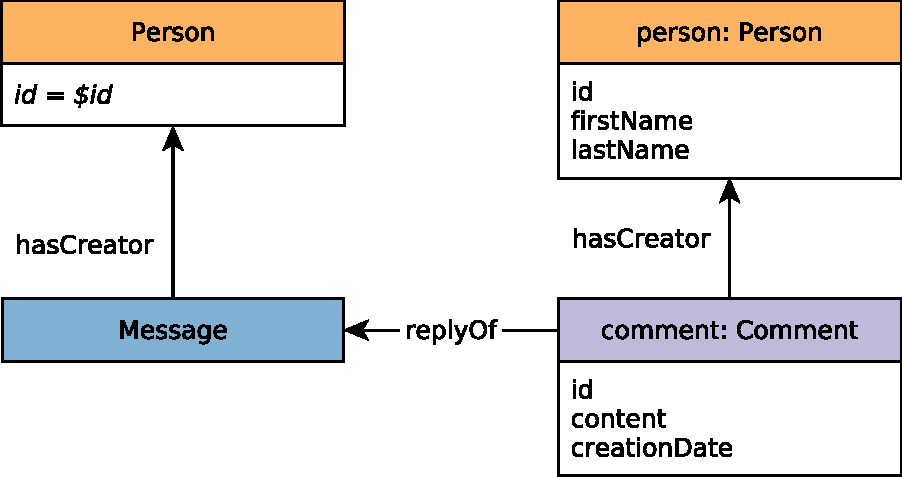
\includegraphics[scale=\patternscale,margin=0cm .2cm]{patterns/interactive08}} \\ \hline
	description & Given a start Person, find (most recent) Comments that are replies to
Messages of the start Person. Only consider immediate (1-hop) replies,
not the transitive (multi-hop) case. Return the reply Comments, and the
Person that created each reply Comment.
 \\ \hline
	
%
	parameters  &
	\vspace{1.1ex}{\begin{tabularx}{14.2cm}{|c|M|m{2cm}|Y|} \hline
	\cellcolor{black!70} \color{white} $\mathsf{1}$ & \varname{Person.id} & \cellcolor{gray!20} \vartype{ID} &  \\ \hline
	\end{tabularx}}\vspace{1.1ex} \\ \hline
%
	result      &
	\vspace{1.1ex}{\begin{tabularx}{14.2cm}{|c|M|m{2cm}|Y|} \hline
	\cellcolor{black!70} \color{white} $\mathsf{1}$ & \varname{Person.id} & \cellcolor{gray!20} \vartype{ID} &  \\ \hline
	\cellcolor{black!70} \color{white} $\mathsf{2}$ & \varname{Person.firstName} & \cellcolor{gray!20} \vartype{String} &  \\ \hline
	\cellcolor{black!70} \color{white} $\mathsf{3}$ & \varname{Person.lastName} & \cellcolor{gray!20} \vartype{String} &  \\ \hline
	\cellcolor{black!70} \color{white} $\mathsf{4}$ & \varname{Comment.creationDate} & \cellcolor{gray!20} \vartype{DateTime} &  \\ \hline
	\cellcolor{black!70} \color{white} $\mathsf{5}$ & \varname{Comment.id} & \cellcolor{gray!20} \vartype{ID} &  \\ \hline
	\cellcolor{black!70} \color{white} $\mathsf{6}$ & \varname{Comment.content} & \cellcolor{gray!20} \vartype{String} &  \\ \hline
	\end{tabularx}}\vspace{1.1ex} \\ \hline
	%
	sort        &
	\vspace{1.1ex}{\begin{tabular}{|c|l|c|} \hline
	\cellcolor{black!70} \color{white} $\mathsf{1}$ & \varname{Comment.creationDate} & \cellcolor{gray!20} $\desc$ \\ \hline
	\cellcolor{black!70} \color{white} $\mathsf{2}$ & \varname{Comment.id} & \cellcolor{gray!20} $\asc$ \\ \hline
	\end{tabular}}\vspace{1.1ex} \\ \hline
	%
	limit       & 20 \\ \hline
	%
	choke points &
	\multicolumn{1}{>{\raggedright}X|}{
		}\\ \hline
\end{tabularx}
\clearpage
\renewcommand*{\arraystretch}{1.1}

\noindent\begin{tabularx}{17cm}{|p{1.95cm}|X|}
	\hline
	workload    & Interactive \\ \hline
%
	query       & 9 \\ \hline
%
	title       & Recent posts and comments by friends or friends of friends \\ \hline
%
    pattern     & \hfill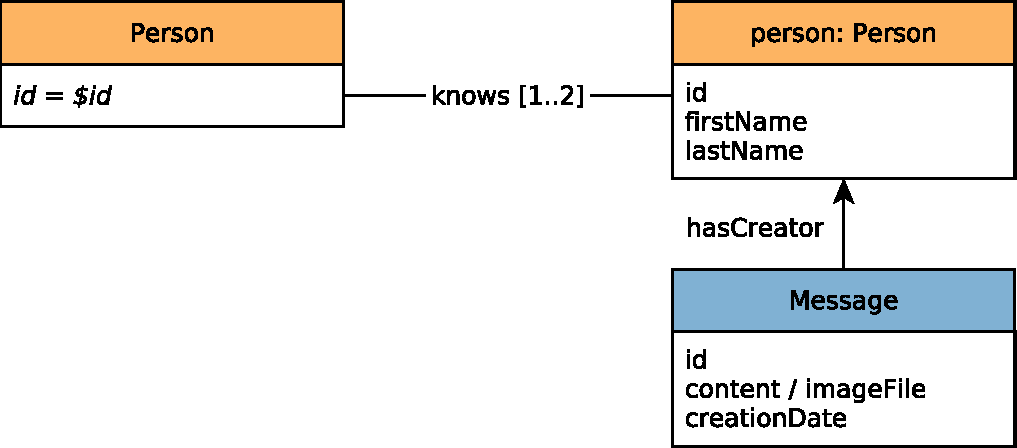
\includegraphics[scale=\patternscale,margin=0cm .2cm]{patterns/interactive09}\hfill\vadjust{} \\ \hline
%
	description & Given a start Person, find the (most recent) Messages created by that
Person's friends or friends of friends (excluding start Person). Only
consider the Messages created before a given date (excluding that date).
 \\ \hline
	
%
	parameters  &
	\vspace{1.1ex}{\begin{tabularx}{14.2cm}{|c|M|m{2cm}|Y|} \hline
	\cellcolor{black!70} \color{white} $\mathsf{1}$ & \varname{Person.id} & \cellcolor{gray!20} \vartype{ID} &  \\ \hline
	\cellcolor{black!70} \color{white} $\mathsf{2}$ & \varname{date} & \cellcolor{gray!20} \vartype{Date} &  \\ \hline
	\end{tabularx}}\vspace{1.1ex} \\ \hline
%
	result      &
	\vspace{1.1ex}{\begin{tabularx}{14.2cm}{|c|M|m{2cm}|Y|} \hline
	\cellcolor{black!70} \color{white} $\mathsf{1}$ & \varname{Message-hasCreator->Person.id} & \cellcolor{gray!20} \vartype{ID} &  \\ \hline
	\cellcolor{black!70} \color{white} $\mathsf{2}$ & \varname{Message-hasCreator->Person.firstName} & \cellcolor{gray!20} \vartype{String} &  \\ \hline
	\cellcolor{black!70} \color{white} $\mathsf{3}$ & \varname{Message-hasCreator->Person.lastName} & \cellcolor{gray!20} \vartype{String} &  \\ \hline
	\cellcolor{black!70} \color{white} $\mathsf{4}$ & \varname{Message.id} & \cellcolor{gray!20} \vartype{ID} &  \\ \hline
	\cellcolor{black!70} \color{white} $\mathsf{5}$ & \varname{Message.content or Post.imageFile} & \cellcolor{gray!20} \vartype{String} &  \\ \hline
	\cellcolor{black!70} \color{white} $\mathsf{6}$ & \varname{Message.creationDate} & \cellcolor{gray!20} \vartype{DateTime} &  \\ \hline
	\end{tabularx}}\vspace{1.1ex} \\ \hline
	%
	sort        &
	\vspace{1.1ex}{\begin{tabular}{|c|l|c|} \hline
	\cellcolor{black!70} \color{white} $\mathsf{1}$ & \varname{Message.creationDate} & \cellcolor{gray!20} $\desc$ \\ \hline
	\cellcolor{black!70} \color{white} $\mathsf{2}$ & \varname{Message.id} & \cellcolor{gray!20} $\asc$ \\ \hline
	\end{tabular}}\vspace{1.1ex} \\ \hline
	%
	limit       & 20 \\ \hline
	%
	choke points &
	\multicolumn{1}{>{\raggedright}X|}{
		}\\ \hline
\end{tabularx}
\clearpage
\renewcommand*{\arraystretch}{1.1}

\noindent\begin{tabularx}{17cm}{|p{1.95cm}|X|}
	\hline
	workload    & Interactive \\ \hline
%
	query       & 10 \\ \hline
%
	title       & Friend recommendation \\ \hline
%
    pattern     & \hfill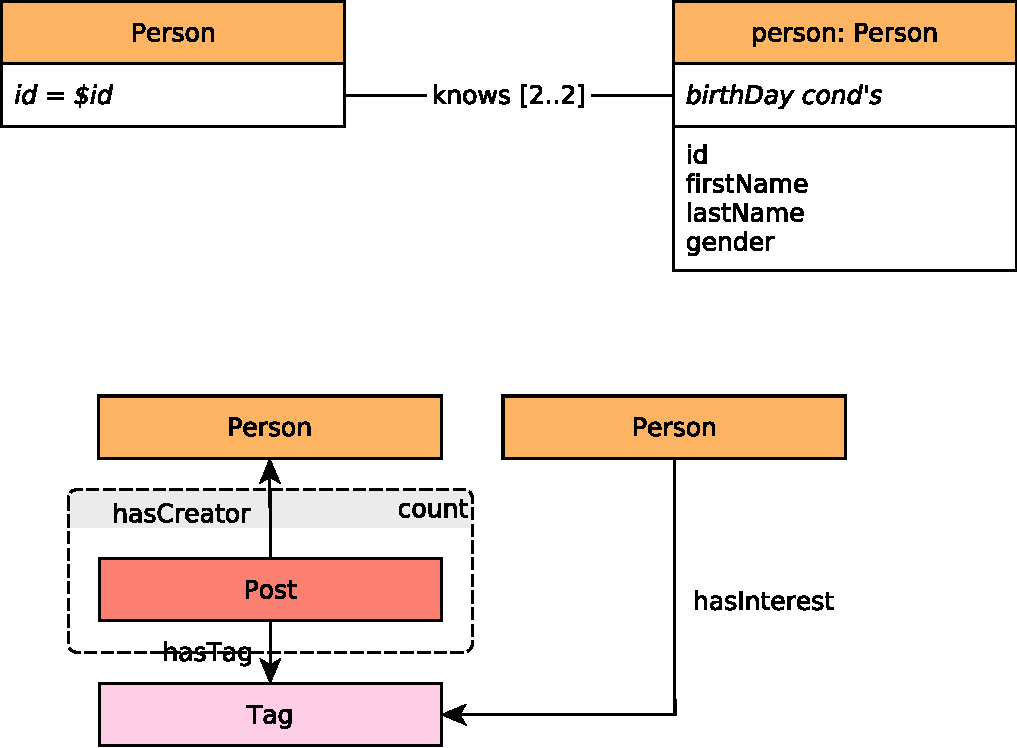
\includegraphics[scale=\patternscale,margin=0cm .2cm]{patterns/interactive10}\hfill\vadjust{} \\ \hline
%
	description & Given a start Person, find that Person's friends of friends (excluding
start Person, and immediate friends), who were born on or after the 21st
of a given month (in any year) and before the 22nd of the following
month. Calculate the similarity between each of these Persons and start
Person, where similarity for any Person is defined as follows:

\begin{itemize}
\tightlist
\item
  common = number of Posts created by that Person, such that the Post
  has a Tag that start Person is Interested in
\item
  uncommon = number of Posts created by that Person, such that the Post
  has no Tag that start Person is Interested in
\item
  similarity = common - uncommon
\end{itemize}
 \\ \hline
	
%
	parameters  &
	\vspace{1.1ex}{\begin{tabularx}{14.2cm}{|c|M|m{2cm}|Y|} \hline
	\cellcolor{black!70} \color{white} $\mathsf{1}$ & \varname{Person.id} & \cellcolor{gray!20} \vartype{ID} &  \\ \hline
	\cellcolor{black!70} \color{white} $\mathsf{2}$ & \varname{month} & \cellcolor{gray!20} \vartype{32-bit Integer} & between 1-12 \\ \hline
	\end{tabularx}}\vspace{1.1ex} \\ \hline
%
	result      &
	\vspace{1.1ex}{\begin{tabularx}{14.2cm}{|c|M|m{2cm}|Y|} \hline
	\cellcolor{black!70} \color{white} $\mathsf{1}$ & \varname{Person.id} & \cellcolor{gray!20} \vartype{ID} &  \\ \hline
	\cellcolor{black!70} \color{white} $\mathsf{2}$ & \varname{Person.firstName} & \cellcolor{gray!20} \vartype{String} &  \\ \hline
	\cellcolor{black!70} \color{white} $\mathsf{3}$ & \varname{Person.lastName} & \cellcolor{gray!20} \vartype{String} &  \\ \hline
	\cellcolor{black!70} \color{white} $\mathsf{4}$ & \varname{similarity} & \cellcolor{gray!20} \vartype{32-bit Integer} &  \\ \hline
	\cellcolor{black!70} \color{white} $\mathsf{5}$ & \varname{Person.gender} & \cellcolor{gray!20} \vartype{String} &  \\ \hline
	\cellcolor{black!70} \color{white} $\mathsf{6}$ & \varname{Person-isLocatedIn->Place.name} & \cellcolor{gray!20} \vartype{String} &  \\ \hline
	\end{tabularx}}\vspace{1.1ex} \\ \hline
	%
	sort        &
	\vspace{1.1ex}{\begin{tabular}{|c|l|c|} \hline
	\cellcolor{black!70} \color{white} $\mathsf{1}$ & \varname{similarity} & \cellcolor{gray!20} $\desc$ \\ \hline
	\cellcolor{black!70} \color{white} $\mathsf{2}$ & \varname{Person.id} & \cellcolor{gray!20} $\asc$ \\ \hline
	\end{tabular}}\vspace{1.1ex} \\ \hline
	%
	limit       & 10 \\ \hline
	%
	choke points &
	\multicolumn{1}{>{\raggedright}X|}{
		}\\ \hline
\end{tabularx}
\clearpage
\renewcommand*{\arraystretch}{1.1}

\noindent\begin{tabularx}{17cm}{|p{1.95cm}|X|}
	\hline
	workload    & interactive \\ \hline
%
	query       & 11 \\ \hline
%
	title       & Job referral \\ \hline
	\multicolumn{2}{|c|}{ 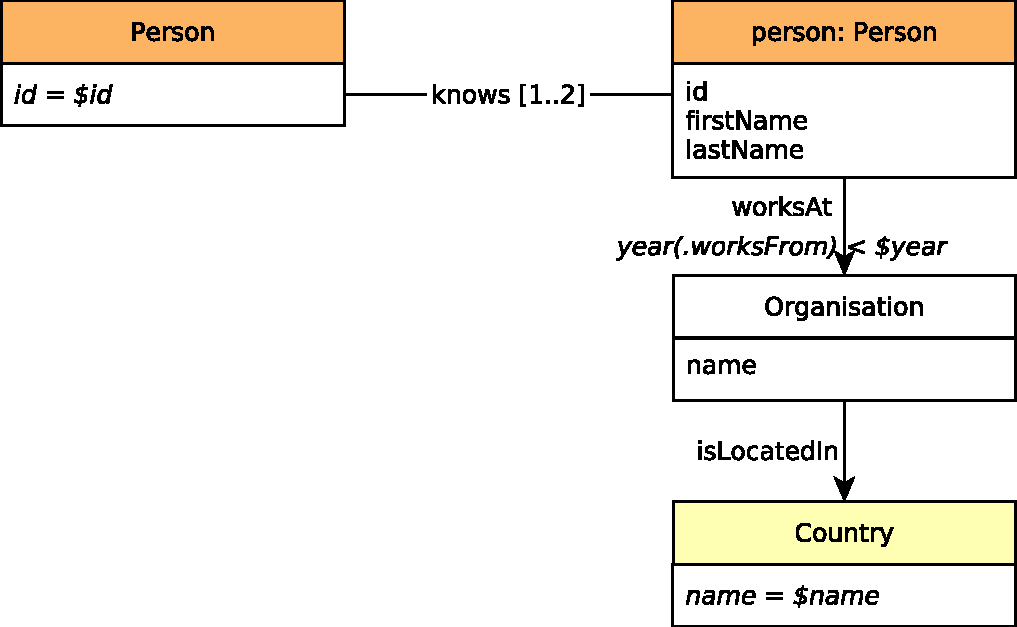
\includegraphics[scale=\patternscale,margin=0cm .2cm]{patterns/interactive11}} \\ \hline
	description & Given a start Person, find that Person's friends and friends of friends
(excluding start Person) who started Working in some Company in a given
Country, before a given date (year).
 \\ \hline
	
%
	parameters  &
	\vspace{1.1ex}{\begin{tabularx}{14.38cm}{|c|M|m{2cm}|Y} \hline
	\cellcolor{black!70} \color{white} $\mathsf{1}$ & \varname{Person.id} & \cellcolor{gray!20} \vartype{ID} &  \\\hline
	\cellcolor{black!70} \color{white} $\mathsf{2}$ & \varname{Country.name} & \cellcolor{gray!20} \vartype{String} &  \\\hline
	\cellcolor{black!70} \color{white} $\mathsf{3}$ & \varname{year} & \cellcolor{gray!20} \vartype{32-bit Integer} &  \\
	\end{tabularx}} \\ \hline
%
	result      &
	\vspace{1.1ex}{\begin{tabularx}{14.38cm}{|c|M|m{2cm}|Y} \hline
	\cellcolor{black!70} \color{white} $\mathsf{1}$ & \varname{Person.id} & \cellcolor{gray!20} \vartype{ID} &  \\\hline
	\cellcolor{black!70} \color{white} $\mathsf{2}$ & \varname{Person.firstName} & \cellcolor{gray!20} \vartype{String} &  \\\hline
	\cellcolor{black!70} \color{white} $\mathsf{3}$ & \varname{Person.lastName} & \cellcolor{gray!20} \vartype{String} &  \\\hline
	\cellcolor{black!70} \color{white} $\mathsf{4}$ & \varname{Person-worksAt->Organization.name} & \cellcolor{gray!20} \vartype{String} &  \\\hline
	\cellcolor{black!70} \color{white} $\mathsf{5}$ & \varname{Person-worksAt->.worksFrom} & \cellcolor{gray!20} \vartype{32-bit Integer} &  \\
	\end{tabularx}} \\ \hline
	%
	sort        &
	\vspace{1.1ex}{\begin{tabular}{|c|l|c|} \hline
	\cellcolor{black!70} \color{white} $\mathsf{1}$ & \varname{Person-worksAt->.worksFrom} & \cellcolor{gray!20} $\asc$ \\\hline
	\cellcolor{black!70} \color{white} $\mathsf{2}$ & \varname{Person.id} & \cellcolor{gray!20} $\asc$ \\\hline
	\cellcolor{black!70} \color{white} $\mathsf{3}$ & \varname{Person-worksAt->Organization.name} & \cellcolor{gray!20} $\desc$ \\
	\end{tabular}} \\ \hline
	%
	limit       & 10 \\ \hline
	%
	choke points &
	\multicolumn{1}{>{\raggedright}X|}{
		}\\ \hline
\end{tabularx}
\clearpage
\renewcommand*{\arraystretch}{1.1}

\noindent\begin{tabularx}{17cm}{|p{1.95cm}|X|}
	\hline
	workload    & interactive \\ \hline
%
	query       & 12 \\ \hline
%
	title       & Expert search \\ \hline
	\multicolumn{2}{|c|}{ 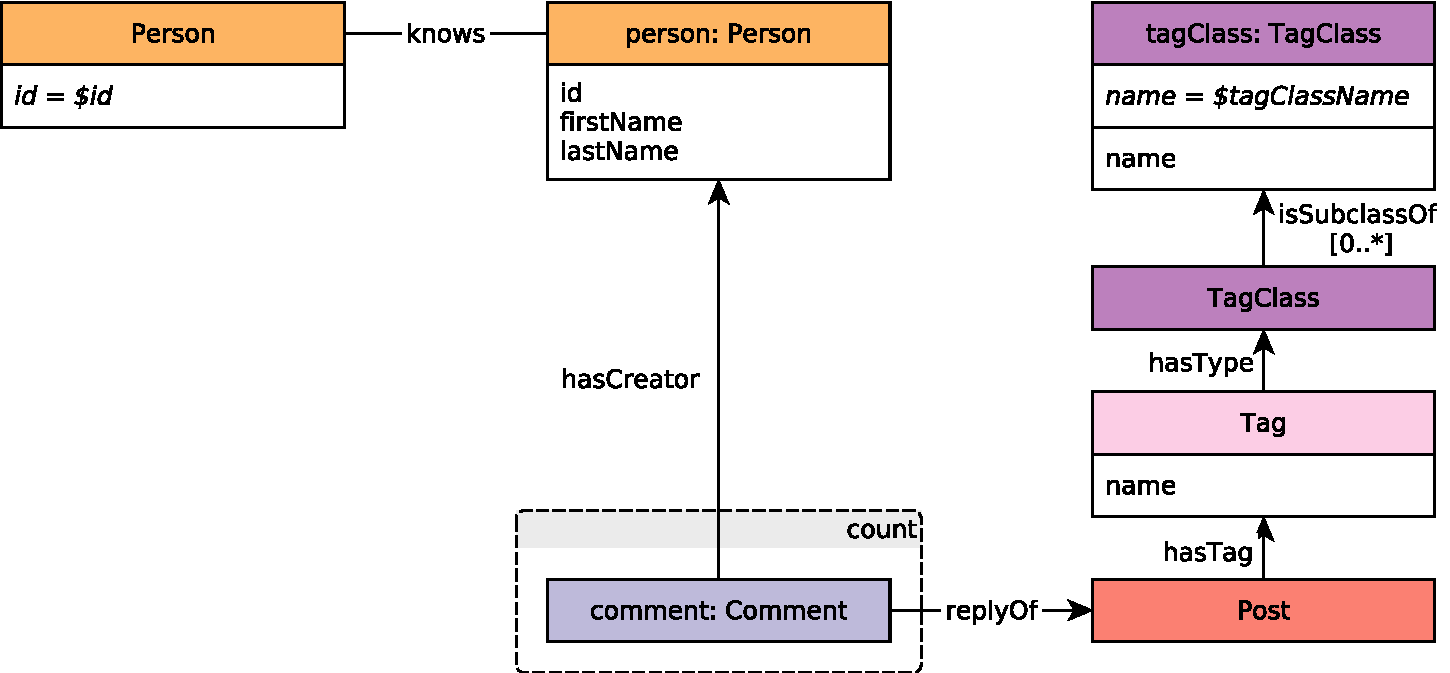
\includegraphics[scale=\patternscale,margin=0cm .2cm]{patterns/interactive12}} \\ \hline
	description & Given a start Person, find the Comments that this Person's friends made
in reply to Posts, considering only those Comments that are immediate
(1-hop) replies to Posts, not the transitive (multi-hop) case. Only
consider Posts with a Tag in a given TagClass or in a descendent of that
TagClass. Count the number of these reply Comments, and collect the Tags
(with valid tag class) that were attached to the Posts they replied to.
Return Persons with at least one reply, the reply count, and the
collection of Tags.
 \\ \hline
	
%
	parameters  &
	\vspace{1.1ex}{\begin{tabularx}{14.38cm}{|c|M|m{2cm}|Y} \hline
	\cellcolor{black!70} \color{white} $\mathsf{1}$ & \varname{Person.id} & \cellcolor{gray!20} \vartype{ID} &  \\\hline
	\cellcolor{black!70} \color{white} $\mathsf{2}$ & \varname{TagClass.name} & \cellcolor{gray!20} \vartype{String} &  \\
	\end{tabularx}} \\ \hline
%
	result      &
	\vspace{1.1ex}{\begin{tabularx}{14.38cm}{|c|M|m{2cm}|Y} \hline
	\cellcolor{black!70} \color{white} $\mathsf{1}$ & \varname{Person.id} & \cellcolor{gray!20} \vartype{ID} &  \\\hline
	\cellcolor{black!70} \color{white} $\mathsf{2}$ & \varname{Person.firstName} & \cellcolor{gray!20} \vartype{String} &  \\\hline
	\cellcolor{black!70} \color{white} $\mathsf{3}$ & \varname{Person.lastName} & \cellcolor{gray!20} \vartype{String} &  \\\hline
	\cellcolor{black!70} \color{white} $\mathsf{4}$ & \varname{\{Tag.name\}} & \cellcolor{gray!20} \vartype{\{String\}} &  \\\hline
	\cellcolor{black!70} \color{white} $\mathsf{5}$ & \varname{count} & \cellcolor{gray!20} \vartype{32-bit Integer} & number of reply Comments \\
	\end{tabularx}} \\ \hline
	%
	sort        &
	\vspace{1.1ex}{\begin{tabular}{|c|l|c|} \hline
	\cellcolor{black!70} \color{white} $\mathsf{1}$ & \varname{count} & \cellcolor{gray!20} $\desc$ \\\hline
	\cellcolor{black!70} \color{white} $\mathsf{2}$ & \varname{Person.id} & \cellcolor{gray!20} $\asc$ \\
	\end{tabular}} \\ \hline
	%
	limit       & 20 \\ \hline
	%
	choke points &
	\multicolumn{1}{>{\raggedright}X|}{
		}\\ \hline
\end{tabularx}
\clearpage
\renewcommand*{\arraystretch}{1.1}

\noindent\begin{tabularx}{17cm}{|p{1.95cm}|X|}
	\hline
	workload    & Interactive \\ \hline
%
	query       & 13 \\ \hline
%
	title       & Single shortest path \\ \hline
	\multicolumn{2}{|c|}{ 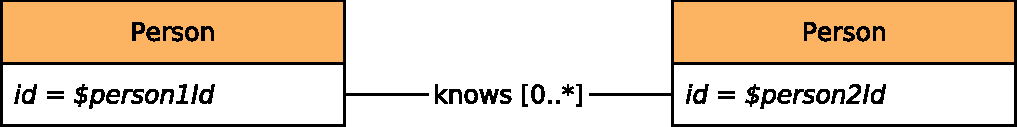
\includegraphics[scale=\patternscale,margin=0cm .2cm]{patterns/interactive13}} \\ \hline
	description & Given two Persons, find the shortest path between these two Persons in
the subgraph induced by the Knows relationships.

Return the length of this path:

\begin{itemize}
\tightlist
\item
  -1 : no path found
\item
  0: start person = end person
\item
  \textgreater{} 0: regular case
\end{itemize}
 \\ \hline
	
%
	parameters  &
	\vspace{1.1ex}{\begin{tabularx}{14.2cm}{|c|M|m{2cm}|Y|} \hline
	\cellcolor{black!70} \color{white} $\mathsf{1}$ & \varname{person1.id} & \cellcolor{gray!20} \vartype{ID} &  \\ \hline
	\cellcolor{black!70} \color{white} $\mathsf{2}$ & \varname{person2.id} & \cellcolor{gray!20} \vartype{ID} &  \\ \hline
	\end{tabularx}}\vspace{1.1ex} \\ \hline
%
	result      &
	\vspace{1.1ex}{\begin{tabularx}{14.2cm}{|c|M|m{2cm}|Y|} \hline
	\cellcolor{black!70} \color{white} $\mathsf{1}$ & \varname{length} & \cellcolor{gray!20} \vartype{32-bit Integer} &  \\ \hline
	\end{tabularx}}\vspace{1.1ex} \\ \hline
	%
	%
	choke points &
	\multicolumn{1}{>{\raggedright}X|}{
		}\\ \hline
\end{tabularx}
\clearpage
\renewcommand*{\arraystretch}{1.1}

\noindent\begin{tabularx}{17cm}{|p{1.95cm}|X|}
	\hline
	workload    & Interactive \\ \hline
%
	query       & 14 \\ \hline
%
	title       & Weighted/unweighted paths \\ \hline
	\multicolumn{2}{|c|}{ 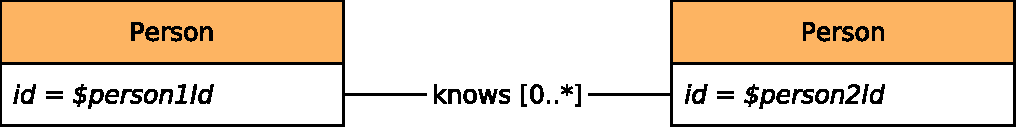
\includegraphics[scale=\patternscale,margin=0cm .2cm]{patterns/interactive14}} \\ \hline
	description & Given two Persons, find all (unweighted) shortest paths between these
two Persons, in the subgraph induced by the Knows relationship. Then,
for each path calculate a weight. The nodes in the path are Persons, and
the weight of a path is the sum of weights between every pair of
consecutive Person nodes in the path. The weight for a pair of Persons
is calculated such that every reply (by one of the Persons) to a Post
(by the other Person) contributes 1.0, and every reply (by ones of the
Persons) to a Comment (by the other Person) contributes 0.5. Return all
the paths with shortest length, and their weights.
 \\ \hline
	
%
	parameters  &
	\vspace{1.1ex}{\begin{tabularx}{14.38cm}{|c|M|m{2cm}|Y} \hline
	\cellcolor{black!70} \color{white} $\mathsf{1}$ & \varname{person1.id} & \cellcolor{gray!20} \vartype{ID} &  \\\hline
	\cellcolor{black!70} \color{white} $\mathsf{2}$ & \varname{person2.id} & \cellcolor{gray!20} \vartype{ID} &  \\
	\end{tabularx}} \\ \hline
%
	result      &
	\vspace{1.1ex}{\begin{tabularx}{14.38cm}{|c|M|m{2cm}|Y} \hline
	\cellcolor{black!70} \color{white} $\mathsf{1}$ & \varname{[Person.id]} & \cellcolor{gray!20} \vartype{[ID]} & Identifiers representing an ordered sequence of the Persons in the path \\\hline
	\cellcolor{black!70} \color{white} $\mathsf{2}$ & \varname{weight} & \cellcolor{gray!20} \vartype{64-bit Float} &  \\
	\end{tabularx}} \\ \hline
	%
	sort        &
	\vspace{1.1ex}{\begin{tabular}{|c|l|c|} \hline
	\cellcolor{black!70} \color{white} $\mathsf{1}$ & \varname{weight} & \cellcolor{gray!20} $\desc$ \\
	\end{tabular}} \\ \hline
	%
	%
	choke points &
	\multicolumn{1}{>{\raggedright}X|}{
		}\\ \hline
\end{tabularx}
\clearpage

\subsection{Short Reads Query Descriptions}

{\small
\begin{enumerate}

  \item Person Profile
    \begin{itemize}
      \item \textbf{Description:}
        Given a start Person, retrieve their first name, last name, birthday, IP address, browser, and city of residence.
      \item \textbf{Parameters:} \\
        \begin{tabular}{lll}
          Person.id 										& ID \\
        \end{tabular}
      \item \textbf{Results:} \\
        \begin{tabular}{lll}
          Person.firstName									& String \\
          Person.lastName										& String \\
          Person.birthDay										& Date \\
          Person.locationIP									& String \\
          Person.browserUsed								& String \\
          Person-isLocatedIn->Place.id			& 32-bit Integer \\
          Person.gender									    & String \\
          Person.creationDate						    & DateTime \\
        \end{tabular}
            \item \textbf{Sort:}
                  \begin{itemize}
                    \item[] -
                  \end{itemize}
            \item \textbf{Limit:}
                  \begin{itemize}
                    \item[] -
                  \end{itemize}
    \end{itemize}

  \item Person Recent Messages
    \begin{itemize}
      \item \textbf{Description:}
        Given a start Person, retrieve the last 10 Messages created by that user.
        For each message, return that message, the original post in its conversation, and the author of that post.
        If any of the Messages is a Post, then the original Post will be the same Message, \ie that Message will appear twice in that result.
      \item \textbf{Parameters:} \\
        \begin{tabular}{lll}
          Person.id 										& ID \\
        \end{tabular}
      \item \textbf{Results:} \\
        \begin{tabular}{lll}
          Message.id     									& 64-bit Integer \\
          Message.content or Post.imageFile										& String \\
          Message.creationDate  & DateTime \\
          Post.id or Comment-replyOf*->Post.id								& ID \\
          Post-hasCreator->Person.id or Comment-replyOf*->Post-hasCreator->Person.id & ID \\
          Post-hasCreator->Person.firstName or Comment-replyOf*->Post-hasCreator->Person.firstName & String \\
          Post-hasCreator->Person.lastName or Comment-replyOf*->Post-hasCreator->Person.lastName & String \\
        \end{tabular}
      \item \textbf{Sort:}
        \begin{itemize}
          \item[1st] Message.creationDate (descending)
          \item[2nd] Message.id (descending)
        \end{itemize}
            \item \textbf{Limit:}
                  \begin{itemize}
                    \item[] -
                  \end{itemize}
    \end{itemize}

  \item Person Friends
    \begin{itemize}
      \item \textbf{Description:}
        Given a start Person, retrieve all of their friends, and the date at which they became friends.
      \item \textbf{Parameters:} \\
        \begin{tabular}{lll}
          Person.id 										& ID \\
        \end{tabular}
      \item \textbf{Results:} \\
        \begin{tabular}{lll}
          Person.id     									& ID \\
          Person.firstName     						& String \\
          Person.lastName    							& String \\
          Knows.creationDate    					& DateTime \\
        \end{tabular}
      \item \textbf{Sort:}
        \begin{itemize}
          \item[1st] Knows.creationDate (descending)
          \item[2nd] Person.id (ascending)
        \end{itemize}
            \item \textbf{Limit:}
                  \begin{itemize}
                    \item[] -
                  \end{itemize}
    \end{itemize}

  \item Message Content
    \begin{itemize}
      \item \textbf{Description:}
        Given a Message, retrieve its content and creation date.
      \item \textbf{Parameters:} \\
        \begin{tabular}{lll}
          Message.id 										& ID \\
        \end{tabular}
      \item \textbf{Results:} \\
        \begin{tabular}{lll}
          Message.creationDate   									& ID \\
          Message.content or Post.imageFile           										& String \\
        \end{tabular}
            \item \textbf{Sort:}
                  \begin{itemize}
                    \item[] -
                  \end{itemize}
            \item \textbf{Limit:}
                  \begin{itemize}
                    \item[] -
                  \end{itemize}
    \end{itemize}

  \item Message Creator
    \begin{itemize}
      \item \textbf{Description:}
        Given a Message, retrieve its author.
      \item \textbf{Parameters:} \\
        \begin{tabular}{lll}
          Message.id 										& ID \\
        \end{tabular}
      \item \textbf{Results:} \\
        \begin{tabular}{lll}
          Message-hasCreator->Person.id     									& ID \\
          Message-hasCreator->Person.firstName     									& String \\
          Message-hasCreator->Person.lastName    									& String \\
        \end{tabular}
            \item \textbf{Sort:}
                  \begin{itemize}
                    \item[] -
                  \end{itemize}
            \item \textbf{Limit:}
                  \begin{itemize}
                    \item[] -
                  \end{itemize}
    \end{itemize}

  \item Message Forum
    \begin{itemize}
      \item \textbf{Description:}
        Given a Message, retrieve the Forum that contains it
        and the Person that moderates that forum. Since comments are not
        directly contained in forums, for comments, return the forum containing
        the original post in the thread which the comment is replying to.
      \item \textbf{Parameters:} \\
        \begin{tabular}{lll}
          Message.id 										& ID \\
        \end{tabular}
      \item \textbf{Results:} \\
        \begin{tabular}{lll}
          Message<-containerOf-Forum.id                       & ID \\
          Message<-containerOf-Forum.title     									& String \\
          Message<-containerOf-Forum-hasModerator->Person.id     									& ID \\
          Message<-containerOf-Forum-hasModerator->Person.firstName    									& String \\
          Message<-containerOf-Forum-hasModerator->Person.lastName    									& String \\
        \end{tabular}
            \item \textbf{Sort:}
                  \begin{itemize}
                    \item[] -
                  \end{itemize}
            \item \textbf{Limit:}
                  \begin{itemize}
                    \item[] -
                  \end{itemize}
    \end{itemize}

  \item Message Replies
    \begin{itemize}
      \item \textbf{Description:}
        Given a Message, retrieve the (1-hop) Comments that reply to it.
        In addition, return a boolean flag indicating if the author of the reply knows the author of the original message.
        If author is same as original author, return false for "knows" flag.
      \item \textbf{Parameters:} \\
        \begin{tabular}{lll}
          Message.id 										& ID \\
        \end{tabular}
      \item \textbf{Results:} \\
        \begin{tabular}{lll}
          Message<-replyOf-Comment.id                       & ID \\
          Message<-replyOf-Comment.content                       & String \\
          Message<-replyOf-Comment.creationDate                       & DateTime \\
          Message-hasCreator->Person.id     									& ID \\
          Message-hasCreator->Person.firstName    									& String \\
          Message-hasCreator->Person.lastName     									& String \\
        \end{tabular}
      \item \textbf{Sort:}
        \begin{itemize}
          \item[1st] Message<-replyOf-Comment.creationDate (descending)
          \item[2nd] Message-hasCreator->Person.id (ascending)
        \end{itemize}
            \item \textbf{Limit:}
                  \begin{itemize}
                    \item[] -
                  \end{itemize}
    \end{itemize}
\end{enumerate}
}


\subsection{Update Query Descriptions}

{\small
\begin{enumerate}
    \item Add Person
        \begin{itemize}
            \item \textbf{Description:} Add a Person to the social network.
            \item \textbf{Parameters:} \\
                \begin{tabular}{lll}
                    Person.id 	 			& ID & \parbox[t]{20cm}{\par \strut} \\
                    Person.firstName 		& String & \parbox[t]{20cm}{\par \strut} \\
                    Person.lastName 		& String & \parbox[t]{20cm}{\par \strut} \\
                    Person.gender 		& String & \parbox[t]{20cm}{\par \strut} \\
                    Person.birthDay 		& Date & \parbox[t]{20cm}{\par \strut} \\
                    Person.creationDate     & DateTime & \parbox[t]{20cm}{\par \strut} \\
                    Person.locationIP     & String & \parbox[t]{20cm}{\par \strut} \\
                    Person.browserUsed     & String & \parbox[t]{20cm}{\par \strut} \\
                    Person-isLocatedIn->City.id 	& ID & \parbox[t]{20cm}{\par \strut} \\
                    Person.speaks 	& \{ String \} & \parbox[t]{20cm}{\par \strut} \\
                    Person.emails 	& \{ String \} & \parbox[t]{20cm}{\par \strut} \\
                    Person-hasInterest->Tag.id 	& \{ ID \} & \parbox[t]{20cm}{\par \strut} \\
                    \{ Person-studyAt->University.id, \\
                    Person-studyAt->.classYear \}  & \{ID, 32-bit Integer\} & \parbox[t]{20cm}{\par \strut} \\
                        \{ Person-workAt->Company.id, \\
                        Person-workAt->.workFrom \}  & \{ID, 32-bit Integer\} & \parbox[t]{20cm}{\par \strut} \\
                        \end{tabular}
                \end{itemize}
            \item Add Post Like
                \begin{itemize}
                    \item \textbf{Description:} Add a Like to a Post of the social network.
                    \item \textbf{Parameters:} \\
                        \begin{tabular}{lll}
                            Person.id 	 			& ID & \parbox[t]{20cm}{\par \strut} \\
                            Post.id 	 			& ID & \parbox[t]{20cm}{\par \strut} \\
                            Person-likes->.creationDate 	 		& DateTime & \parbox[t]{20cm}{\par \strut} \\
                        \end{tabular}
                \end{itemize}
            \item Add Comment Like
                \begin{itemize}
                    \item \textbf{Description: Add a Like to a Comment of the social network.}
                    \item \textbf{Parameters:} \\
                        \begin{tabular}{lll}
                            Person.id 	 			& ID & \parbox[t]{20cm}{\par \strut} \\
                            Comment.id 	 			& ID & \parbox[t]{20cm}{\par \strut} \\
                            Person-likes->.creationDate 	 		& DateTime & \parbox[t]{20cm}{\par \strut} \\
                        \end{tabular}
                \end{itemize}
            \item Add Forum
                \begin{itemize}
                    \item \textbf{Description:} Add a Forum to the social network.
                    \item \textbf{Parameters:} \\
                        \begin{tabular}{lll}
                            Forum.id 	 			& ID & \parbox[t]{20cm}{// person 1\strut} \\
                            Forum.title 	 			& String & \parbox[t]{20cm}{// person 2\strut} \\
                            Forum.creationDate & DateTime & \parbox[t]{20cm}{\par \strut} \\
                            Forum-hasModerator->Person.id 	& \{ ID \} & \parbox[t]{20cm}{\par \strut} \\
                            Forum-hasTag->Tag.id 	& \{ ID \} & \parbox[t]{20cm}{\par \strut} \\
                        \end{tabular}
                \end{itemize}
            \item Add Forum Membership
                \begin{itemize}
                    \item \textbf{Description:} Add a Forum membership to the social network.
                    \item \textbf{Parameters:} \\
                        \begin{tabular}{lll}
                            Person.id 	 			& ID & \parbox[t]{20cm}{\par \strut} \\
                            Person-hasMember->Forum.id 	 			& ID & \parbox[t]{20cm}{\par \strut} \\
                            Person-hasMember->.joinDate 	 		& DateTime & \parbox[t]{20cm}{\par \strut} \\
                        \end{tabular}
                \end{itemize}
            \item Add Post
                \begin{itemize}
                    \item \textbf{Description:} Add a Post to the social network.
                    \item \textbf{Parameters:} \\
                        \begin{tabular}{lll}
                            Post.id 	 			& ID & \parbox[t]{20cm}{\par \strut} \\
                            Post.imageFile 	 			& String & \parbox[t]{20cm}{\par \strut} \\
                            Post.creationDate 	 		& DateTime & \parbox[t]{20cm}{\par \strut} \\
                            Post.locationIP 	 		& String & \parbox[t]{20cm}{\par \strut} \\
                            Post.browserUsed 	 		& String & \parbox[t]{20cm}{\par \strut} \\
                            Post.language 	 		    & String & \parbox[t]{20cm}{\par \strut} \\
                            Post.content 	 		    & Text & \parbox[t]{20cm}{\par \strut} \\
                            Post.length 	 		    & 32-bit Integer & \parbox[t]{20cm}{\par \strut} \\
                            Post-hasCreator->Person.id & ID & \parbox[t]{20cm}{\par \strut} \\
                            Forum-containerOf->Post.id & ID & \parbox[t]{20cm}{\par \strut} \\
                            Post-isLocatedIn->Country.id & ID & \parbox[t]{20cm}{\par \strut} \\
                            \{Post-hasTag->Tag.id\} & \{ID\} & \parbox[t]{20cm}{\par \strut} \\
                        \end{tabular}
                \end{itemize}
            \item Add Comment
                \begin{itemize}
                    \item \textbf{Description:} Add a Comment replying to a Post/Comment to the social network.
                    \item \textbf{Parameters:} \\
                        \begin{tabular}{lll}
                            Comment.id 	 			& ID & \parbox[t]{20cm}{\par \strut} \\
                            Comment.creationDate 			& DateTime & \parbox[t]{20cm}{\par \strut} \\
                            Comment.locationIP 	 		& String & \parbox[t]{20cm}{\par \strut} \\
                            Comment.browserUsed 	 		& String & \parbox[t]{20cm}{\par \strut} \\
                            Comment.content 	 		    & Text & \parbox[t]{20cm}{\par \strut} \\
                            Comment.length 	 		    & 32-bit Integer & \parbox[t]{20cm}{\par \strut} \\
                            Comment-hasCreator->Person.id & ID & \parbox[t]{20cm}{\par \strut} \\
                            Comment-isLocatedIn->Country.id & ID & \parbox[t]{20cm}{\par \strut} \\
                            Comment-replyOf->Post.id & ID & \parbox[t]{20cm}{ // -1 if the comment is a reply of a comment. \strut} \\
                            Comment-replyOf->Comment.id & ID & \parbox[t]{20cm}{// -1 if the comment is a reply of a post. \strut} \\
                            \{Comment-hasTag->Tag.id\} & \{ID\} & \parbox[t]{20cm}{\par \strut} \\
                        \end{tabular}
                \end{itemize}
            \item Add Friendship
                \begin{itemize}
                    \item \textbf{Description:} Add a friendship relation to the social network
                    \item \textbf{Parameters:} \\
                        \begin{tabular}{lll}
                            Person.id 	 			& ID & \parbox[t]{20cm}{// person 1\strut} \\
                            Person.id 	 			& ID & \parbox[t]{20cm}{// person 2\strut} \\
                            Person-knows->.creationDate & DateTime & \parbox[t]{20cm}{\par \strut} \\
                        \end{tabular}
                \end{itemize}
        \end{enumerate}
      }


\section{Substitution parameters}\label{section:substitution}
Together with the dataset, DATAGEN produces a set of parameters per
query type. Parameter generation is designed in such a way that for each query
type, all of the generated parameters yield similar runtime behaviour of that
query.

Specifically, the selection of parameters for a query template guarantees the following properties of the resulting queries:
\begin{enumerate}
\item[P1:] the query runtime has a bounded variance: the average runtime corresponds to the behavior of the majority of the queries
\item[P2:] the runtime distribution is stable: different samples of (\eg 10) parameter bindings used in different query streams result in an identical runtime distribution across streams
\item[P3:] the optimal logical plan (optimal operator order) of the queries is the same: this ensures that a specific query template tests the system's behavior under the well-chosen technical difficulty (\eg handling voluminous joins or proper cardinality estimation for subqueries, \etc)
\end{enumerate}


As a result, the amount of data that the query touches is roughly the
same for every parameter binding, assuming that the query optimizer figures out a
reasonable execution plan for the query. This is done to avoid bindings that
cause unexpectedly long or short runtimes of queries, or even result in a
completely different optimal execution plan. Such effects could arise due to
the data skew and correlations between values in the generated dataset.

In order to get the parameter bindings for each of the queries, we have designed a \textit{Parameter Curation} procedure that works in two stages:

\begin{enumerate}
\item for each query template for all possible parameter bindings, we determine the size of intermediate results in the {\em intended} query plan. Intermediate result size heavily influences the runtime of a query, so two queries with the same operator tree and similar intermediate result sizes at every level of this operator tree are expected to have similar runtimes. This analysis is effectively a side effect of data generation, that is we keep all the necessary counts (number of friends per user, number of posts of friends \etc) as we create the dataset.
\item then, a greedy algorithm selects (``curates'') those parameters with similar intermediate result counts from the domain of all the parameters.
\end{enumerate}

Parameter bindings are stored in the \texttt{substitution\_parameters} folder
inside the data generator directory. Each query gets its bindings in a separate
file. Every line of a parameter file is a JSON-formatted collection of
key-value pairs (name of the parameter and its value). For example, the Query 1
parameter bindings are stored in file \texttt{query\_1\_param.txt}, and one of
its lines may look like this:

\vspace{-6mm}
$$
\{\text{"PersonID"}: 1, \text{"Name"}: \text{"Lei"}, \text{"PersonURI"}: \text{"http://www.ldbc.eu/ldbc\_socialnet/1.0/data/pers1"}\}
$$

Depending on implementation, the SUT may refer to persons either by IDs
(relational and graph databases) or URIs (RDF systems), so we provide both
values for the Person parameter.  Finally, parameters for short reads are taken
from those in complex reads and updates.


\section{Load Definition}\label{section:workload}
\ldbcsnb Test Driver is in charge of the execution of the Interactive Workload.
At the beginning of the execution, the Test Driver creates a query mix by
assigning to each query instance, a query issue time and a set of parameters
taken from the generated substitution parameter set described above.  

Query issue times have to be carefully assigned.  Although substitution
parameters are chosen in such a way that queries of the same type take similar
time, not all query types have the same complexity and touch the same amount of
data, which causes them to scale differently for the different scale factors.
Therefore, if all query instances, regardless of their type, are issued
at the same rate, those more complex queries will dominate the execution's
result, making faster query types purposeless. To avoid this situation, each
query type is executed at a different rate. The way the execution rate is decided,
also depends on the nature of the query: complex read, short read or update.

Update queries' issue times are taken from the update streams generated by the
data generator. These are the times where the actual event happened during the
simulation of the social network. Complex reads' times are expressed in terms
of update operations. For each complex read query type, a frequency value is
assigned which specifies the relation between the number of updates performed
per complex read.  Table~\ref{table:freqs} shows the frequencies assigned to
each query type for SF1. The frequencies of the different scale factors can be
found in Appendix~\ref{appendix:scale_factors}.

\begin{table}[H]
\centering
    \begin{tabular}{|c|c|c|c|}
    \hline
    Query Type & freq & Query Type & freq \\ 
    \hline
    \hline
    Query 1 & 26 & Query 8 & 45 \\ 
    \hline       
    Query 2 & 37 & Query 9 & 157 \\  
    \hline        
    Query 3 & 69 & Query 10 & 30 \\ 
    \hline        
    Query 4 & 36 & Query 11 & 16 \\ 
    \hline        
    Query 5 & 57 & Query 12 & 44 \\ 
    \hline        
    Query 6 & 129 & Query 13 & 19 \\  
    \hline        
    Query 7 & 87 & Query 14 & 49 \\ 
    \hline
    \end{tabular}
    \caption{Frequencies for each query type for SF1.}
    \label{table:freqs}
\end{table}

Finally, short reads are inserted in order to balance the ratio between reads
and writes, and to simulate the behavior of a real user of the social network.
For each complex read instance, a sequence of short reads is planned. There are two
types of short read sequences: Person centric and Message centric. Depending on
the type of the complex read, one of them is chosen. Each sequence consists of
a set of short reads which are issued in a row. The issue time assigned to each
short read in the sequence is determined at run time, and is based on the
completion time of the complex read it depends on. 
The substitution parameters for short reads are taken from the results of previously
executed complex reads and short reads.
Once a short read sequence is issued (and provided that sufficient substitution parameters 
exist), there is a probability that another short read  sequence is issued. 
This probability decreases for each new sequence issued. 
Since the same random number generator seed is used across
executions, the workload is deterministic.


The specified frequencies, implicitly define the query ratios between queries
of different types, as well as a default target throughput. However the Test
Sponsor may specify a different target throughput to test,  by ``squeezing''
together or ``stretching'' apart the queries of the workload. This is
achieved  by means of the ``Time Compression Ratio'' that is multiplied by the
frequencies (see \autoref{table:freqs}).  Therefore, different
throughputs can be tested while maintaining the relative ratios between the
different query types.


\chapter{Business Intelligence Workload}

\section{Choke Points}
\section{Choke Points}

\subsection{Aggregation Performance}

\subsubsection{SNBI-1.1/TCPH-1.2: [QOPT]  Interesting Orders}
\label{choke_point_1.1}
This choke-point tests the ability of the query optimizer to exploit the interesting orders induced by some operators. Apart from clustered indexes providing key order, other operators also preserve or even induce tuple orderings.
Sort-based operators create new orderings, typically the probe-side of a hash join conserves its order, etc.

\subsubsection{SNBI-1.2/TCPH-1.1: [QEXE] High Cardinality group-by performance}
\label{choke_point_1.2}
This choke-point tests the ability of the execution engine to parallelize group-by's with a large number of groups. Some queries require performing large group-by's.
In such a case, if an aggregation produces a significant number of groups, intra query parallelization can be exploited as each thread may make its own partial aggregation.
Then, to produce the result, these have to be re-aggregated. In order to avoid this, the tuples entering the aggregation operator may be partitioned by a hash of the grouping key and be sent to the appropriate partition.
Each partition would have its own thread so that only that thread would write the aggregation, hence avoiding costly critical sections as well. A high cardinality distinct modifier in a query is a special case of this choke point.
It is amenable to the same solution with intra query parallelization and partitioning as the group-by.
We further note that scale-out systems have an extra incentive for partitioning since this will distribute the CPU and memory pressure over multiple machines, yielding better platform utilization and scalability.

\subsubsection{SNBI-1.3: [QEXE] Complex aggregate performance}
\label{choke_point_1.3}
This choke-point test the performance of the execution engine to perform complex aggregates. Many databases offer user defined aggregates and more complex aggregation operations than the basic count, sum, max and min, for example string concatenation aggregation operator. These types of aggregates are expected to benefit from the same optimizations as the basic built-in ones, for example partitioning.

\subsubsection{SNBI-1.4: [QOPT]  Top-k push down}
\label{choke_point_1.4}
Top-k push down. This choke-point tests the ability of the query optimizer to perform optimizations based on top-k selections. Many times queries demand for returning the top-k elements.
Once k results are obtained, extra restrictions in a selection can be added based on the properties of the kth element currently in the top-k, being more restrictive as the query advances, instead of sorting all elements and picking the highest k.

\subsubsection{SNBI-1.5/TCPH-1.4: [QEXE] Dependent group-by keys}
\label{choke_point_1.5}
This choke-point tests the ability of the query optimizer to exclude those functionally dependent group-bys. Sometimes queries require for group-by's on a set of columns and a key, where the value of the key determines the columns.
In this situation, the aggregation operator should be able to exclude certain group-by attributes from the key matching.

\subsubsection{SNBI-1.6/TCPH-1.3: [QEXE] Low Cardinality group-by performance}
\label{choke_point_1.6}
This choke-point tests the ability to efficiently perform group by evaluation when only a very limited set of groups is available.  This can require special strategies for parallelization, e.g. pre-aggregation when possible. This case also allows using special strategies for grouping like using array lookup if the domain of keys is small.

\subsection{Join Performance}

\subsubsection{SNBI-2.1/TCPH-2.3: [QOPT]  Rich join order optimization}
\label{choke_point_2.1}
This choke-point tests the ability of the query optimizer to find optimal join orders. A graph can be traversed in different ways. In the relational model, this is equivalent as different join orders.
The execution time of these orders may differ by orders of magnitude. Therefore, finding an efficient join (traversal) order is important, which in general, requires enumeration of all the possibilities.
The enumeration is complicated by operators that are not freely re-orderable like semi-, \mbox{anti-,} and outer-joins. Because of this difficulty most join enumeration algorithms do not enumerate all possible plans, and therefore can miss the optimal join order. Therefore, these chokepoint tests the ability of the query optimizer to find optimal join (traversal) orders.

\subsubsection{SNBI-2.2/TCPH-2.4: [QOPT]  Late projection}
\label{choke_point_2.2}
This choke-point tests the ability of the query optimizer to delay the projection of unneeded attributes until late in the execution. Queries where certain columns are only needed late in the query.
In such a situation, it is better to omit them from initial table scans, as fetching them later by row-id with a separate scan operator, which is joined to the intermediate query result, can save temporal space, and therefore I/O.
Late projection does have a trade-off involving locality, since late in the plan the tuples may be in a different order, and scattered I/O in terms of tuples/second is much more expensive than sequential I/O.
Late projection specifically makes sense in queries where the late use of these columns happens at a moment where the amount of tuples involved has been considerably reduced;
for example after an aggregation with only few unique group-by keys, or a top-k operator.

\subsubsection{SNBI-2.3/TCPH-2.1: [QOPT]  Join type selection}
\label{choke_point_2.3}
This choke-point tests the ability of the query optimizer to select the proper join operator type, which implies accurate estimates of cardinalities.
Depending on the cardinalities of both sides of a join, a hash or an index index based join operator is more appropriate.
This is especially important with column stores, where one usually has an index on everything. Deciding to use a hash join requires a good estimation of cardinalities on both the probe and build sides.
In TPC-H, the use of hash join is almost a foregone conclusion in many cases, since an implementation will usually not even define an index on foreign key columns.
There is a break even point between index and hash based plans, depending on the cardinality on the probe and build sides

\subsubsection{SNBI-2.4/TCPH-2.2: [QOPT]  Sparse foreign key joins}
\label{choke_point_2.4}
This choke-point tests the performance of join operators when the join is sparse. Sometimes joins involve relations where only a small percentage of rows in one of the tables is required to satisfy a join. When tables are larger, typical join methods can be sub-optimal. Partitioning the sparse table, using Hash Clustered indexes or implementing bloom filter tests inside the join are techniques to improve the performance in such situations~\cite{DBLP:journals/csur/Graefe93}.

\subsection{Data Access Locality}

\subsubsection{SNBI-3.1/TCPH-3.3: [QOPT]  Detecting correlation}
\label{choke_point_3.1}
This choke-point tests the ability of the query optimizer to detect data correlations and exploiting them. If a schema rewards creating clustered indexes, the question then is which of the date or data columns to use as key.
In fact it should not matter which column is used, as range- propagation between correlated attributes of the same table is relatively easy. One way is through the creation of multi-attribute histograms after detection of attribute correlation.
With MinMax indexes, range-predicates on any column can be translated into qualifying tuple position ranges. If an attribute value is correlated with tuple position, this reduces the area to scan roughly equally to predicate selectivity.

\subsubsection{SNBI-3.2: [STORAGE] Dimensional clustering}
\label{choke_point_3.2}
This chokepoint tests suitability of the identifiers assigned to entities by the storage system to better exploit data locality. A data model where each entity has a unique synthetic identifier,
e.g. RDF or graph models, has some choice in assigning a value to this identifier. The properties of the entity being identified may affect this, e.g. type (label), other dependent properties,
e.g. geographic location, date, position in a hierarchy etc, depending on the application. Such identifier choice may create locality which in turn improves efficiency of compression or index access.

\subsubsection{SNBI-3.3: [QEXE] Scattered Index Access patterns}
\label{choke_point_3.3}
This choke-point tests the performance of indexes when scattered accesses are performed. The efficiency of index lookup is very different depending on the locality of keys coming to the indexed access.
Techniques like vectoring non-local index accesses by simply missing the cache in parallel on multiple lookups vectored on the same thread may have high impact.
Also detecting absence of locality should turn off any locality dependent optimizations if these are costly when there is no locality. A graph neighborhood traversal is an example of an operation with random access without predictable locality.

\subsection{Expression Calculation}

\subsubsection{SNBI-4.1/TPCH-4.2a: [QOPT]  Common subexpression elimination}
\label{choke_point_4.1}
This choke-point tests the ability of the query optimizer to detect common sub-expressions and reuse their results. A basic technique helpful in multiple queries is common subexpression elimination (CSE).
CSE should recognize also that average aggregates can be derived afterwards by dividing a SUM by the COUNT when those have been computed.

\subsubsection{SNBI-4.2/TCPH-4.2d: [QOPT]  Complex boolean expression joins and selections}
\label{choke_point_4.2}
This choke-point tests the ability of the query optimizer to reorder the execution of boolean expressions to improve the performance. Some boolean expressions are complex, with possibilities for alternative optimal evaluation orders.
For instance, the optimizer may reorder conjunctions to test first those conditions with larger selectivity~\cite{DBLP:conf/vldb/Moerkotte98}.

\subsubsection{SNBI-4.3 [QEXE] Low overhead expressions interpretation}
\label{choke_point_4.3}
This choke-point tests the ability to efficiently evaluate simple expressions on a large number of values. A typical example could be simple arithmetic expressions, mathematical functions like floor and absolute or date functions like extracting a year.

\subsection{Correlated Sub-queries}

\subsubsection{SNBI-5.1/TCPH-5.1: [QOPT]  Flattening sub-queries}
\label{choke_point_5.1}
This choke-point tests the ability of the query optimizer to flatten execution plans when there are correlated sub-queries. Many queries have correlated sub-queries and their query plans can be flattened,
such that the correlated sub-query is handled using an equi-join, outer-join or anti-join. To execute queries well, systems need to flatten both sub-queries, the first into an equi-join plan, the second into an anti-join plan.
Therefore, the execution layer of the database system will benefit from implementing these extended join variants.
The ill effects of repetitive tuple-at-a-time sub-query execution can also be mitigated if execution systems by using vectorized, or block-wise query execution, allowing to run sub-queries with thousands of input parameters instead of one.
The ability to look up many keys in an index in one API call creates the opportunity to benefit from physical locality, if lookup keys exhibit some clustering.

\subsubsection{SNBI-5.2/TCPH-5.3: [QEXE] Overlap between outer and sub-query}
\label{choke_point_5.2}
This choke-point tests the ability of the execution engine to reuse results when there is an overlap between the outer query and the sub-query. In some queries, the correlated sub-query and the outer query have the same joins and selections.
In this case, a non-tree, rather DAG-shaped~\cite{DBLP:conf/btw/NeumannM09} query plan would allow to execute the common parts just once, providing the intermediate result stream to both the outer query and correlated sub-query,
which higher up in the query plan are joined together (using normal query decorrelation rewrites).
As such, the benchmark rewards systems where the optimizer can detect this and the execution engine supports an operator that can buffer intermediate results and provide them to multiple parent operators.

\subsubsection{SNBI-5.3/TCPH-5.2 ? TODO: [QEXE] Intra-query result reuse}
\label{choke_point_5.3}
This choke-point tests the ability of the execution engine to reuse sub-query results when two sub-queries are mostly identical.
Some queries have almost identical sub-queries, where some of their internal results can be reused in both sides of the execution plan, thus avoiding to repeat computations.

\subsection{Parallelism and Concurrency}

\subsubsection{SNBI-6.1/TCPH-6.3: [QEXE] Inter-query result reuse}
\label{choke_point_6.1}
This choke-point tests the ability of the query execution engine to reuse results from different queries. Sometimes with a high number of streams a significant amount of identical queries emerge in the resulting workload.
The reason is that certain parameters, as generated by the workload generator, have only a limited amount of parameters bindings.
This weakness opens up the possibility of using a query result cache, to eliminate the repetitive part of the workload.
A further opportunity that detects even more overlap is the work on recycling, which does not only cache final query results, but also intermediate query results of a "high worth".
Here, worth is a combination of partial-query result size, partial-query evaluation cost, and observed (or estimated) frequency of the partial-query in the workload.

\subsection{RDF and Graph Specifics}

\subsubsection{SNBI-7.1: [QOPT]  Translation of internal ids to external ones [KILL WITH FIRE]}
\label{choke_point_7.1}
This choke-point tests the ability of the query optimizer to delay the translation between internal and external entity ids to late in the query. Translate at point of minimum cardinality,
e.g. after top k order by RDF and possibly graph models often use a synthetic integer identifier for entities, e.g. URI's . For presentation to the client applications, these identifiers must be translated to their original form,
e.g. the URI string that was used when loading the data. This should be done as late as possible, or at the point of minimal cardinality in the plan.

\subsubsection{SNBI-7.2: [QOPT]  Cardinality estimation of transitive paths}
\label{choke_point_7.2}
This choke-point tests the ability of the query optimizer to properly estimate the cardinality of intermediate results when executing transitive paths. A transitive path may occur in a ``fact table'' or a ``dimension table'' position.
A transitive path may cover a tree or a graph, e.g. descendants in a geographical hierarchy vs. graph neighborhood or transitive closure in a many-to-many connected social network.
In order to decide proper join order and type, the cardinality of the expansion of the transitive path needs to be correctly estimated.
This could for example take the form of executing on a sample of the data in the cost model or of gathering special statistics, e.g. the depth and fan-out of a tree. In the case of hierarchical dimensions,
e.g. geographic locations or other hierarchical classifications, detecting the cardinality of the transitive path will allow one to go to a star schema plan with scan of a fact table with a selective hash join.
Such a plan will be on the other hand very bad for example if the hash table is much larger than the ``fact table'' being scanned.

\subsubsection{SNBI-7.3: [QEXE] Execution of a transitive step}
\label{choke_point_7.3}
This choke-point tests the ability of the query execution engine to efficiently execute transitive steps. Graph workloads may have transitive operations, for example finding a shortest path between vertices.
This involves repeated execution of a short lookup, often on many values at the same time, while usually having an end condition, e.g. the target vertex being reached or having reached the border of a search going in the opposite direction.
For the best efficiency, these operations can be merged or tightly coupled to the index operations themselves. Also parallelization may be possible but may need to deal with a global state, e.g. set of visited vertices.
There are many possible tradeoffs between generality and performance

\subsubsection{SNBI 7.4: [QEXE] Efficient evaluation of termination criteria for transitive queries}
\label{choke_point_7.4}
This tests the ability of a system to express termination criteria for transitive queries so that not the whole transitive relation has to be evaluated as well as efficient testing for termination.

\subsubsection{SNBI 7.5: [QEXE] Path pattern reuse}
\label{choke_point_7.5}
This choke-point tests the ability of the execution engine to reuse work across graph traversals [TODO: complete in more detail]
For example, when computing paths within a range of distances, it is often possible to incrementally compute longer paths by reusing paths of shorter distances that were already computed


\section{Graph Patterns}

We use the following notation for defining graph patterns:

\begin{itemize}
	\item Filtering conditions are typeset in \textit{italic}.
	\item Properties that should be returned are denoted in normal (book) font.
	\item Negative conditions, i.e., edges that are now allowed in the graph are denoted with dashed \textcolor{red}{red} lines.
	\item Aggregations are shown in dashed boxes.
\end{itemize}

\begin{figure}[hbp]
	\begin{center}
		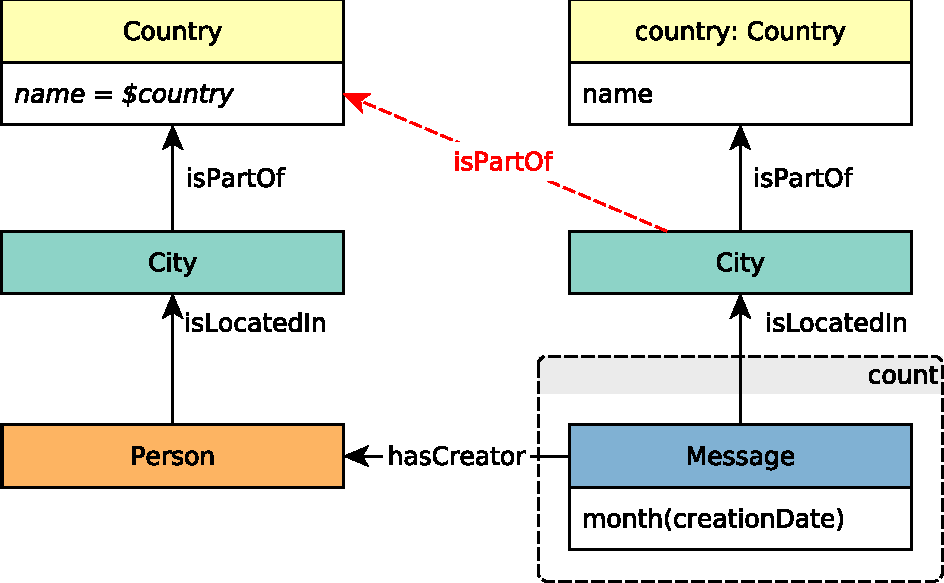
\includegraphics[scale=\patternscale,margin=0cm .2cm]{patterns/q23}
		\caption{Example graph pattern.}
		\label{fig:example-graph-pattern}
	\end{center}
\end{figure}



\section{Business Intelligence Queries}

\clearpage

\renewcommand*{\arraystretch}{1.1}

\noindent\begin{tabularx}{17cm}{|p{1.95cm}|X|}
	\hline
	workload    & BI \\ \hline
%
	query       & 1 \\ \hline
%
	title       & Posting summary \\ \hline
	\multicolumn{2}{|c|}{ 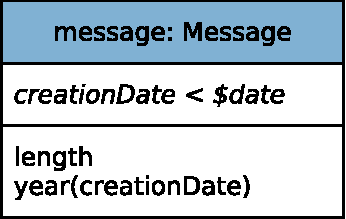
\includegraphics[scale=\patternscale,margin=0cm .2cm]{patterns/bi01}} \\ \hline
	description & Given a date, find all Messages created before that date. Group them by
a 3-level grouping:

\begin{enumerate}
\def\labelenumi{\arabic{enumi}.}
\tightlist
\item
  by year of creation
\item
  for each year, group into message types, i.e., Posts or Comments
\item
  for each year-type group, split into four groups based on length of
  their content

  \begin{itemize}
  \tightlist
  \item
    0 \textless{}= length \textless{} 40: \texttt{short}
  \item
    40 \textless{}= length \textless{} 80: \texttt{one\ liner}
  \item
    80 \textless{}= length \textless{} 160: \texttt{tweet}
  \item
    160 \textless{}= length: \texttt{long}
  \end{itemize}
\end{enumerate}
 \\ \hline
	
%
	group by       &
	\multicolumn{1}{>{\raggedright}X|}{
		\varname{year}, 
		\varname{message type}, 
		\varname{length group}
		} \\ \hline
	
%
	parameters  &
	\vspace{1.1ex}{\begin{tabularx}{14.2cm}{|c|M|m{2cm}|Y|} \hline
	\cellcolor{black!70} \color{white} $\mathsf{1}$ & \varname{date} & \cellcolor{gray!20} \vartype{Date} &  \\ \hline
	\end{tabularx}}\vspace{1.1ex} \\ \hline
%
	result      &
	\vspace{1.1ex}{\begin{tabularx}{14.2cm}{|c|M|m{2cm}|Y|} \hline
	\cellcolor{black!70} \color{white} $\mathsf{1}$ & \varname{message.year} & \cellcolor{gray!20} \vartype{32-bit Integer} &  \\ \hline
	\cellcolor{black!70} \color{white} $\mathsf{2}$ & \varname{messageType} & \cellcolor{gray!20} \vartype{String} & post/comment (in lowercase) \\ \hline
	\cellcolor{black!70} \color{white} $\mathsf{3}$ & \varname{lengthCategory} & \cellcolor{gray!20} \vartype{String} & short/one-liner/tweet/long (in lowercase) \\ \hline
	\cellcolor{black!70} \color{white} $\mathsf{4}$ & \varname{messageCount} & \cellcolor{gray!20} \vartype{32-bit Integer} & total number of Messages (Posts/Comments) in that group \\ \hline
	\cellcolor{black!70} \color{white} $\mathsf{5}$ & \varname{averageMessageLength} & \cellcolor{gray!20} \vartype{32-bit Integer} & average length of the Message content in that group \\ \hline
	\cellcolor{black!70} \color{white} $\mathsf{6}$ & \varname{sumMessageLength} & \cellcolor{gray!20} \vartype{32-bit Integer} & sum of all message content lengths \\ \hline
	\cellcolor{black!70} \color{white} $\mathsf{7}$ & \varname{percentageOfMessages} & \cellcolor{gray!20} \vartype{32-bit Float} & number of messages in group as a percentage of all messages created before the given date \\ \hline
	\end{tabularx}}\vspace{1.1ex} \\ \hline
	%
	sort        &
	\vspace{1.1ex}{\begin{tabular}{|c|l|c|} \hline
	\cellcolor{black!70} \color{white} $\mathsf{1}$ & \varname{year} & \cellcolor{gray!20} $\desc$ \\ \hline
	\cellcolor{black!70} \color{white} $\mathsf{2}$ & \varname{message type} & \cellcolor{gray!20} $\asc$ \\ \hline
	\cellcolor{black!70} \color{white} $\mathsf{3}$ & \varname{size category} & \cellcolor{gray!20} $\asc$ \\ \hline
	\end{tabular}}\vspace{1.1ex} \\ \hline
	%
	%
	choke points &
	\multicolumn{1}{>{\raggedright}X|}{
		\chokepoint{1.2}, 
		\chokepoint{3.2}, 
		\chokepoint{4.1}
		}\\ \hline
\end{tabularx}
\clearpage
\renewcommand*{\arraystretch}{1.5}
\noindent\begin{tabularx}{17cm}{|p{1.95cm}|X|}
	\hline
	number      & 2                                                          \\ \hline
	title       & Top tags for country, age, gender, time                                                           \\ \hline
	\multicolumn{2}{|c|}{ 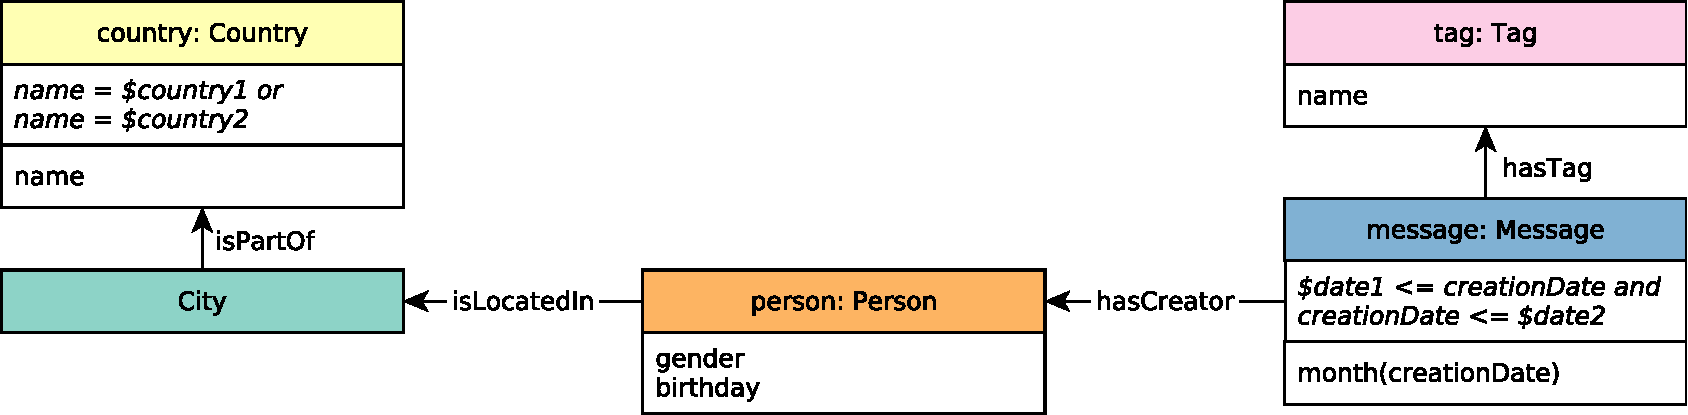
\includegraphics[scale=\patternscale,margin=0cm .2cm]{patterns/q02}} \\ \hline
	description & Select all Messages (Posts \& Comments) created between date1-date2
(inclusive) by persons located in country1 or country2. Select the
creators (Persons) and the Tags of these Messages. Split these Persons,
Tags and Messages into a 5-level grouping: (1) name of country of
person, (2) month message was created, (3) gender of person, (4) age
group of person, defined as years between person's birthday and end of
simulation (2013-01-01), divided by 5, rounded down, (5) name of tag
attached to message.

Only return groups where number of messages is greater than 100.
 \\ \hline
	
	group by       &
	\multicolumn{1}{>{\raggedright}X|}{
		\varname{countryName}, 
		\varname{month}, 
		\varname{gender}, 
		\varname{ageGroup}, 
		\varname{tagName}
		}\\ \hline
	
	parameters  &
	\renewcommand*{\arraystretch}{1.0}
	\vspace{-1.8ex}{\begin{tabularx}{14.2cm}{|c|l|p{2cm}|Y|} \hline
	\cellcolor{black!70} \color{white} $\mathsf{1}$ & \varname{date1} & \cellcolor{gray!20} \vartype{Date} & \\ \hline
	\cellcolor{black!70} \color{white} $\mathsf{2}$ & \varname{date2} & \cellcolor{gray!20} \vartype{Date} & \\ \hline
	\cellcolor{black!70} \color{white} $\mathsf{3}$ & \varname{country1} & \cellcolor{gray!20} \vartype{String} & \\ \hline
	\cellcolor{black!70} \color{white} $\mathsf{4}$ & \varname{country2} & \cellcolor{gray!20} \vartype{String} & \\ 
	\end{tabularx}} \\ \hline
	result      &
	\renewcommand*{\arraystretch}{1.0}
	\vspace{-1.8ex}{\begin{tabularx}{14.2cm}{|c|l|p{2cm}|Y|} \hline
	\cellcolor{black!70} \color{white} $\mathsf{1}$ & \varname{country.name} & \cellcolor{gray!20} \vartype{String} & \\ \hline
	\cellcolor{black!70} \color{white} $\mathsf{2}$ & \varname{message.month} & \cellcolor{gray!20} \vartype{32bitInteger} & \\ \hline
	\cellcolor{black!70} \color{white} $\mathsf{3}$ & \varname{person.gender} & \cellcolor{gray!20} \vartype{String} & \\ \hline
	\cellcolor{black!70} \color{white} $\mathsf{4}$ & \varname{ageGroup} & \cellcolor{gray!20} \vartype{32bitInteger} & \\ \hline
	\cellcolor{black!70} \color{white} $\mathsf{5}$ & \varname{tag.name} & \cellcolor{gray!20} \vartype{String} & \\ \hline
	\cellcolor{black!70} \color{white} $\mathsf{6}$ & \varname{messageCount} & \cellcolor{gray!20} \vartype{64bitInteger} & \\ 
	\end{tabularx}} \\ \hline
	sort        &
	\renewcommand*{\arraystretch}{1.0}
	\vspace{-1.8ex}{\begin{tabular}{|c|l|c|} \hline
	\cellcolor{black!70} \color{white} $\mathsf{1}$ & \varname{messageCount} & \cellcolor{gray!20} $\desc$ \\ \hline
	\cellcolor{black!70} \color{white} $\mathsf{2}$ & \varname{tag.name} & \cellcolor{gray!20} $\asc$ \\ \hline
	\cellcolor{black!70} \color{white} $\mathsf{3}$ & \varname{ageGroup} & \cellcolor{gray!20} $\asc$ \\ \hline
	\cellcolor{black!70} \color{white} $\mathsf{4}$ & \varname{person.gender} & \cellcolor{gray!20} $\asc$ \\ \hline
	\cellcolor{black!70} \color{white} $\mathsf{5}$ & \varname{message.month} & \cellcolor{gray!20} $\asc$ \\ \hline
	\cellcolor{black!70} \color{white} $\mathsf{6}$ & \varname{country.name} & \cellcolor{gray!20} $\asc$ \\ 
	\end{tabular}} \\ \hline
	limit       & 100                                                           \\ \hline
	choke points        &
	\multicolumn{1}{>{\raggedright}X|}{
		\chokepoint{1.1}, 
		\chokepoint{1.2}, 
		\chokepoint{1.4}, 
		\chokepoint{2.1}, 
		\chokepoint{2.3}, 
		\chokepoint{3.1}, 
		\chokepoint{3.2}
		}\\ \hline
\end{tabularx}
\clearpage
\renewcommand*{\arraystretch}{1.1}

\noindent\begin{tabularx}{17cm}{|p{1.95cm}|X|}
	\hline
	workload    & BI \\ \hline
%
	query       & 3 \\ \hline
%
	title       & Tag evolution \\ \hline
	\multicolumn{2}{|c|}{ 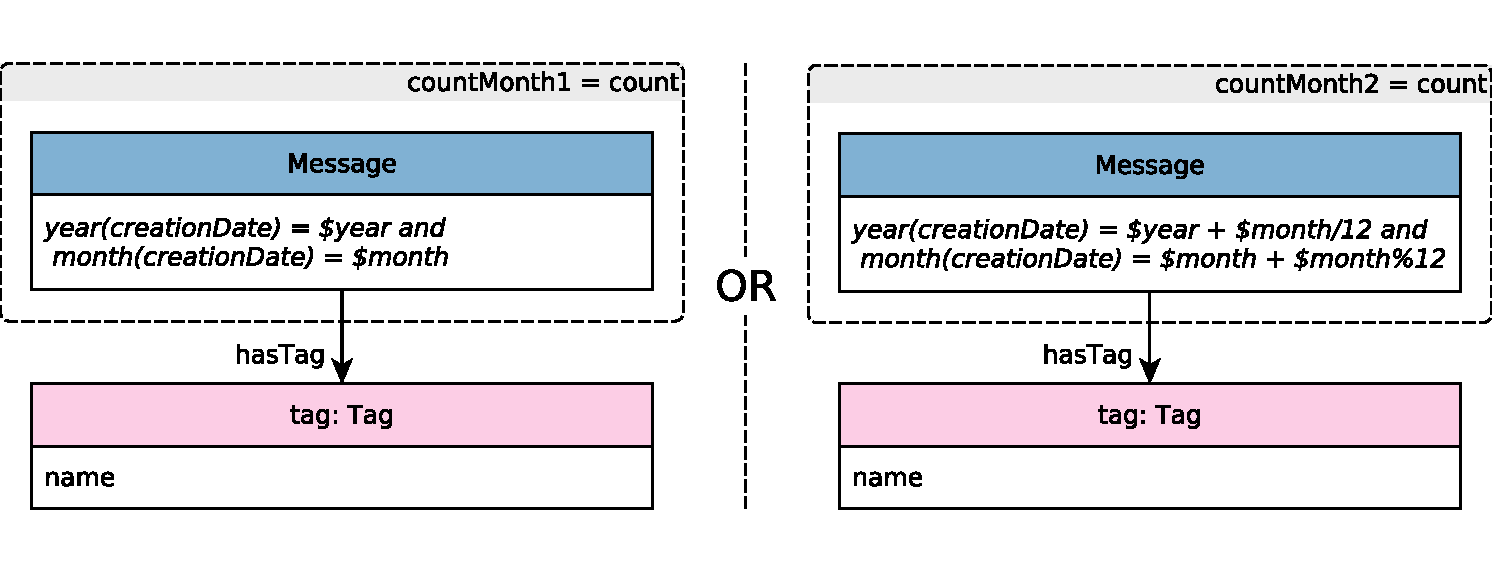
\includegraphics[scale=\patternscale,margin=0cm .2cm]{patterns/bi03}} \\ \hline
	description & Given a year and a month, find the Tags that were used in Messages
during the given month of the given year, and the Tags that were used
during the month after the given month of the given year.

For both months, compute the count of Messages that used each of the
Tags.
 \\ \hline
	
%
	parameters  &
	\vspace{1.1ex}{\begin{tabularx}{14.38cm}{|c|M|m{2cm}|Y} \hline
	\cellcolor{black!70} \color{white} $\mathsf{1}$ & \varname{year} & \cellcolor{gray!20} \vartype{32-bit Integer} &  \\\hline
	\cellcolor{black!70} \color{white} $\mathsf{2}$ & \varname{month} & \cellcolor{gray!20} \vartype{32-bit Integer} &  \\
	\end{tabularx}} \\ \hline
%
	result      &
	\vspace{1.1ex}{\begin{tabularx}{14.38cm}{|c|M|m{2cm}|Y} \hline
	\cellcolor{black!70} \color{white} $\mathsf{1}$ & \varname{tag.name} & \cellcolor{gray!20} \vartype{String} &  \\\hline
	\cellcolor{black!70} \color{white} $\mathsf{2}$ & \varname{countMonth1} & \cellcolor{gray!20} \vartype{32-bit Integer} & occurrences of the tag during year-month 1 \\\hline
	\cellcolor{black!70} \color{white} $\mathsf{3}$ & \varname{countMonth2} & \cellcolor{gray!20} \vartype{32-bit Integer} & occurrences of the tag during year-month 2 \\\hline
	\cellcolor{black!70} \color{white} $\mathsf{4}$ & \varname{diff} & \cellcolor{gray!20} \vartype{32-bit Integer} & difference between occurrences of this Tag in month 1 and month 2 \\
	\end{tabularx}} \\ \hline
	%
	sort        &
	\vspace{1.1ex}{\begin{tabular}{|c|l|c|} \hline
	\cellcolor{black!70} \color{white} $\mathsf{1}$ & \varname{diff} & \cellcolor{gray!20} $\desc$ \\\hline
	\cellcolor{black!70} \color{white} $\mathsf{2}$ & \varname{tag.name} & \cellcolor{gray!20} $\asc$ \\
	\end{tabular}} \\ \hline
	%
	limit       & 100 \\ \hline
	%
	choke points &
	\multicolumn{1}{>{\raggedright}X|}{
		\chokepoint{2.4}, 
		\chokepoint{3.1}, 
		\chokepoint{3.2}, 
		\chokepoint{4.1}, 
		\chokepoint{4.3}, 
		\chokepoint{5.3}, 
		\chokepoint{6.1}
		}\\ \hline
\end{tabularx}
\clearpage
\renewcommand*{\arraystretch}{1.1}

\noindent\begin{tabularx}{17cm}{|p{1.95cm}|X|}
	\hline
	workload    & BI \\ \hline
%
	query       & 4 \\ \hline
%
	title       & Popular topics in a country \\ \hline
	\multicolumn{2}{|c|}{ 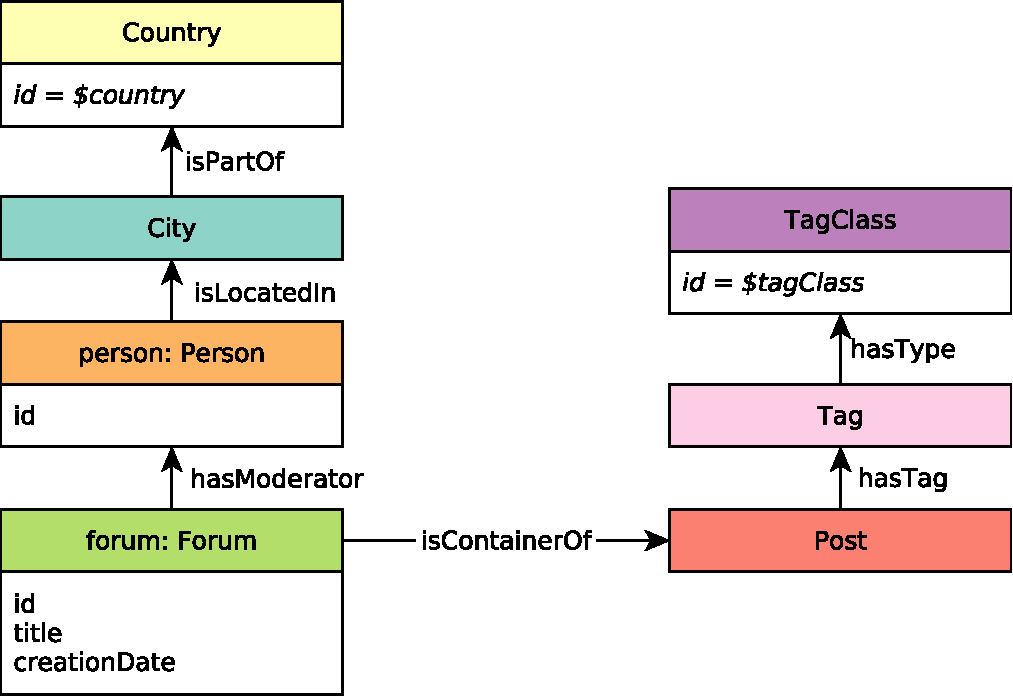
\includegraphics[scale=\patternscale,margin=0cm .2cm]{patterns/bi04}} \\ \hline
	description & Given a TagClass and a Country, find all the Forums created in the given
Country, containing at least one Post with Tags belonging directly to
the given TagClass.

The location of a Forum is identified by the location of the Forum's
moderator.

TODO - what do we count, Posts? (szarnyasg)
 \\ \hline
	
%
	parameters  &
	\vspace{1.1ex}{\begin{tabularx}{14.38cm}{|c|M|m{2cm}|Y} \hline
	\cellcolor{black!70} \color{white} $\mathsf{1}$ & \varname{tagClass} & \cellcolor{gray!20} \vartype{32-bit Integer} &  \\\hline
	\cellcolor{black!70} \color{white} $\mathsf{2}$ & \varname{country} & \cellcolor{gray!20} \vartype{32-bit Integer} &  \\
	\end{tabularx}} \\ \hline
%
	result      &
	\vspace{1.1ex}{\begin{tabularx}{14.38cm}{|c|M|m{2cm}|Y} \hline
	\cellcolor{black!70} \color{white} $\mathsf{1}$ & \varname{forum.id} & \cellcolor{gray!20} \vartype{64-bit Integer} &  \\\hline
	\cellcolor{black!70} \color{white} $\mathsf{2}$ & \varname{forum.title} & \cellcolor{gray!20} \vartype{String} &  \\\hline
	\cellcolor{black!70} \color{white} $\mathsf{3}$ & \varname{forum.creationDate} & \cellcolor{gray!20} \vartype{DateTime} &  \\\hline
	\cellcolor{black!70} \color{white} $\mathsf{4}$ & \varname{person.id} & \cellcolor{gray!20} \vartype{64-bit Integer} &  \\\hline
	\cellcolor{black!70} \color{white} $\mathsf{5}$ & \varname{count} & \cellcolor{gray!20} \vartype{32-bit Integer} &  \\
	\end{tabularx}} \\ \hline
	%
	sort        &
	\vspace{1.1ex}{\begin{tabular}{|c|l|c|} \hline
	\cellcolor{black!70} \color{white} $\mathsf{1}$ & \varname{count} & \cellcolor{gray!20} $\desc$ \\\hline
	\cellcolor{black!70} \color{white} $\mathsf{2}$ & \varname{forum.id} & \cellcolor{gray!20} $\asc$ \\
	\end{tabular}} \\ \hline
	%
	limit       & 20 \\ \hline
	%
	choke points &
	\multicolumn{1}{>{\raggedright}X|}{
		\chokepoint{1.1}, 
		\chokepoint{1.2}, 
		\chokepoint{1.4}, 
		\chokepoint{2.1}, 
		\chokepoint{2.2}, 
		\chokepoint{2.4}, 
		\chokepoint{3.3}
		}\\ \hline
\end{tabularx}
\clearpage
\renewcommand*{\arraystretch}{1.1}

\noindent\begin{tabularx}{17cm}{|p{1.95cm}|X|}
	\hline
	workload    & BI \\ \hline
%
	query       & 5 \\ \hline
%
	title       & Top posters in a country \\ \hline
	\multicolumn{2}{|c|}{ 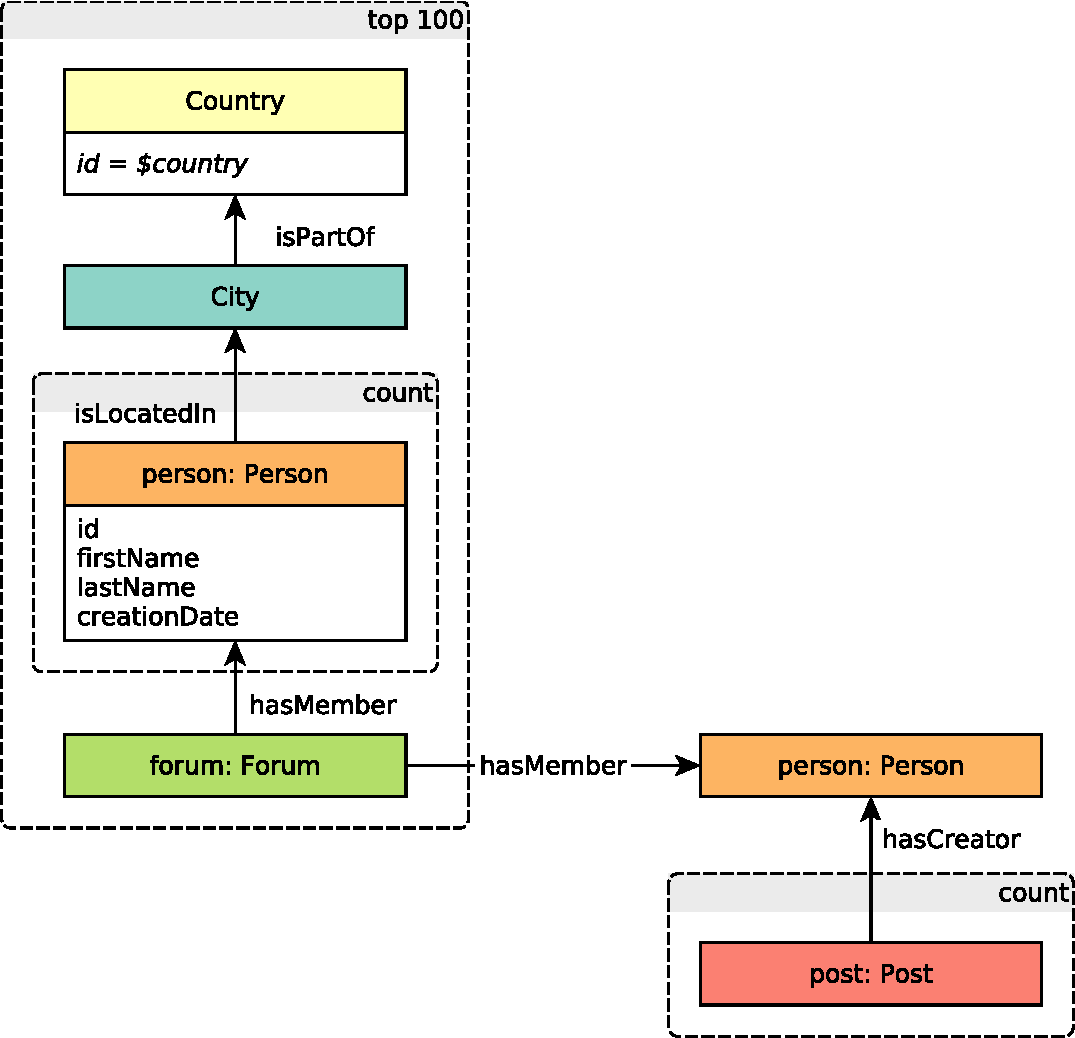
\includegraphics[scale=\patternscale,margin=0cm .2cm]{patterns/bi05}} \\ \hline
	description & Find the most popular Forums for a given Country, where the popularity
of a Forum is measured by the number of members that Forum has from the
given Country.

For each member of the 100 most popular Forums, count the number of
Posts they made in any of those (most popular) Forums.
 \\ \hline
	
%
	group by       &
	\multicolumn{1}{>{\raggedright}X|}{
		\varname{person.id}, 
		\varname{person.firstName}, 
		\varname{person.lastName}, 
		\varname{person.creationDate}
		} \\ \hline
	
%
	parameters  &
	\vspace{1.1ex}{\begin{tabularx}{14.2cm}{|c|M|m{2cm}|Y|} \hline
	\cellcolor{black!70} \color{white} $\mathsf{1}$ & \varname{country} & \cellcolor{gray!20} \vartype{32-bit Integer} &  \\ \hline
	\end{tabularx}}\vspace{1.1ex} \\ \hline
%
	result      &
	\vspace{1.1ex}{\begin{tabularx}{14.2cm}{|c|M|m{2cm}|Y|} \hline
	\cellcolor{black!70} \color{white} $\mathsf{1}$ & \varname{person.id} & \cellcolor{gray!20} \vartype{64-bit Integer} &  \\ \hline
	\cellcolor{black!70} \color{white} $\mathsf{2}$ & \varname{person.firstName} & \cellcolor{gray!20} \vartype{String} &  \\ \hline
	\cellcolor{black!70} \color{white} $\mathsf{3}$ & \varname{person.lastName} & \cellcolor{gray!20} \vartype{String} &  \\ \hline
	\cellcolor{black!70} \color{white} $\mathsf{4}$ & \varname{person.creationDate} & \cellcolor{gray!20} \vartype{DateTime} &  \\ \hline
	\cellcolor{black!70} \color{white} $\mathsf{5}$ & \varname{postCount} & \cellcolor{gray!20} \vartype{32-bit Integer} &  \\ \hline
	\end{tabularx}}\vspace{1.1ex} \\ \hline
	%
	sort        &
	\vspace{1.1ex}{\begin{tabular}{|c|l|c|} \hline
	\cellcolor{black!70} \color{white} $\mathsf{1}$ & \varname{postCount} & \cellcolor{gray!20} $\desc$ \\ \hline
	\cellcolor{black!70} \color{white} $\mathsf{2}$ & \varname{person.id} & \cellcolor{gray!20} $\asc$ \\ \hline
	\end{tabular}}\vspace{1.1ex} \\ \hline
	%
	limit       & 100 \\ \hline
	%
	choke points &
	\multicolumn{1}{>{\raggedright}X|}{
		\chokepoint{1.2}, 
		\chokepoint{1.4}, 
		\chokepoint{1.5}, 
		\chokepoint{2.1}, 
		\chokepoint{2.2}, 
		\chokepoint{2.3}, 
		\chokepoint{2.4}, 
		\chokepoint{3.3}, 
		\chokepoint{5.3}, 
		\chokepoint{6.1}
		}\\ \hline
\end{tabularx}
\clearpage
\renewcommand*{\arraystretch}{1.5}
\noindent\begin{tabularx}{17cm}{|p{1.95cm}|X|}
	\hline
	number      & 6                                                          \\ \hline
	title       & Most active Posters of a given Topic                                                           \\ \hline
	\multicolumn{2}{|c|}{ 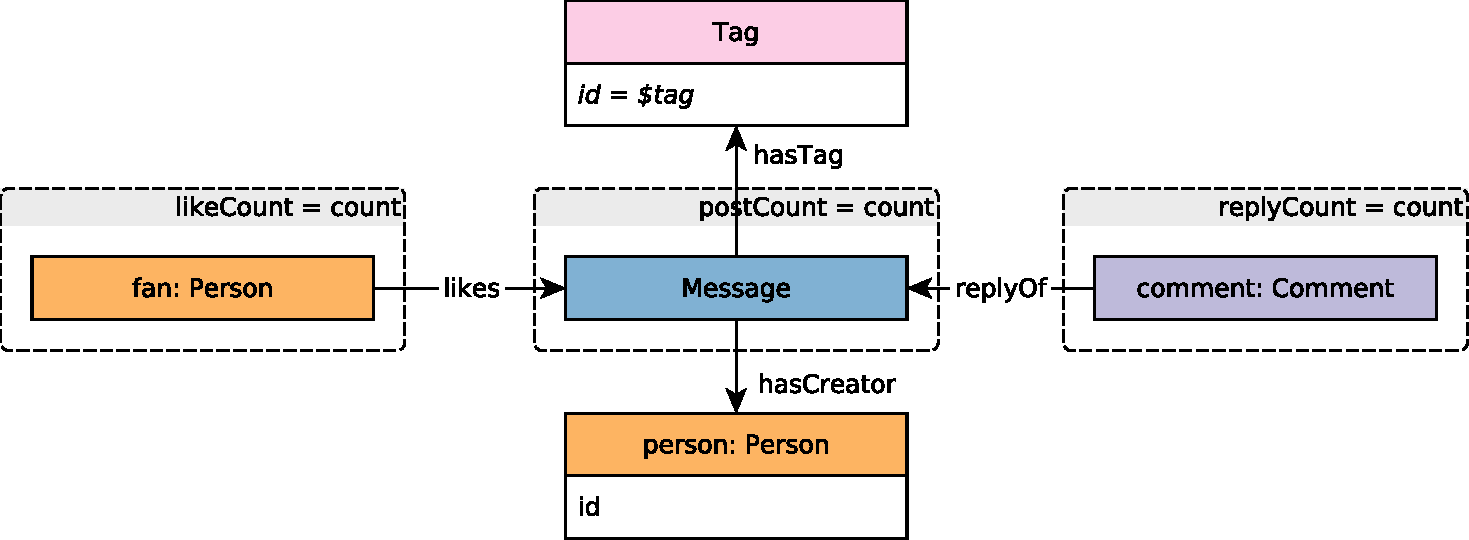
\includegraphics[scale=\patternscale,margin=0cm .2cm]{patterns/q06}} \\ \hline
	description & Get Persons who have created a Message (Post or Comment) with a given
Tag.

Each Person has a score, computed as follows:

\begin{itemize}
\tightlist
\item
  Count of Messages with the given Tag (\texttt{postCount}).
\item
  Count of Likes (\texttt{likeCount}) and Comments (\texttt{replyCount})
  in reply of their Messages with the given Tag. (TODO - transitive or
  direct? szarnyasg)
\end{itemize}

The sum is weighted as follows:

\begin{itemize}
\tightlist
\item
  Messages (\texttt{postCount}) are multiplied by 1,
\item
  Comments to Messages (\texttt{replyCount}) are multiplied by 2,
\item
  Likes (\texttt{likeCount}) are multiplied by 10.
\end{itemize}
 \\ \hline
	
	parameters  &
	\renewcommand*{\arraystretch}{1.0}
	\vspace{-1.8ex}{\begin{tabularx}{14.2cm}{|c|l|p{2cm}|Y|} \hline
	\cellcolor{black!70} \color{white} $\mathsf{1}$ & \varname{tag} & \cellcolor{gray!20} \vartype{32bitInteger} & \\ 
	\end{tabularx}} \\ \hline
	result      &
	\renewcommand*{\arraystretch}{1.0}
	\vspace{-1.8ex}{\begin{tabularx}{14.2cm}{|c|l|p{2cm}|Y|} \hline
	\cellcolor{black!70} \color{white} $\mathsf{1}$ & \varname{person.id} & \cellcolor{gray!20} \vartype{64bitInteger} & \\ \hline
	\cellcolor{black!70} \color{white} $\mathsf{2}$ & \varname{replyCount} & \cellcolor{gray!20} \vartype{32bitInteger} & \\ \hline
	\cellcolor{black!70} \color{white} $\mathsf{3}$ & \varname{likeCount} & \cellcolor{gray!20} \vartype{32bitInteger} & \\ \hline
	\cellcolor{black!70} \color{white} $\mathsf{4}$ & \varname{postCount} & \cellcolor{gray!20} \vartype{32bitInteger} & \\ \hline
	\cellcolor{black!70} \color{white} $\mathsf{5}$ & \varname{score} & \cellcolor{gray!20} \vartype{32bitInteger} & \\ 
	\end{tabularx}} \\ \hline
	sort        &
	\renewcommand*{\arraystretch}{1.0}
	\vspace{-1.8ex}{\begin{tabular}{|c|l|c|} \hline
	\cellcolor{black!70} \color{white} $\mathsf{1}$ & \varname{score} & \cellcolor{gray!20} $\desc$ \\ \hline
	\cellcolor{black!70} \color{white} $\mathsf{2}$ & \varname{person.id} & \cellcolor{gray!20} $\asc$ \\ 
	\end{tabular}} \\ \hline
	limit       & 100                                                           \\ \hline
	choke points        &
	\multicolumn{1}{>{\raggedright}X|}{
		\chokepoint{1.2}, 
		\chokepoint{2.3}
		}\\ \hline
\end{tabularx}
\clearpage
\renewcommand*{\arraystretch}{1.1}

\noindent\begin{tabularx}{17cm}{|p{1.95cm}|X|}
	\hline
	number      & 7                                                          \\ \hline
%
	title       & Most authoritative users on a given topic                                                           \\ \hline
	\multicolumn{2}{|c|}{ 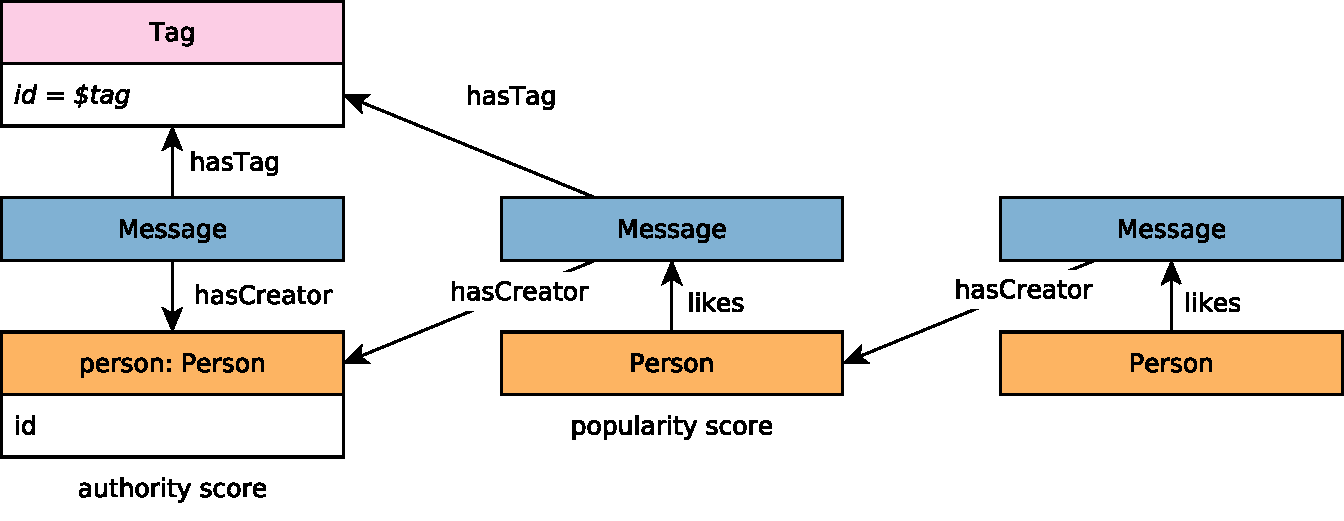
\includegraphics[scale=\patternscale,margin=0cm .2cm]{patterns/q07}} \\ \hline
	description & Given a Tag, find all Persons that ever created a Message with the given
Tag. For each of these Persons compute their ``authority score'' as
follows:

\begin{itemize}
\tightlist
\item
  The ``authority score'' is the sum of ``popularity scores'' of the
  Persons that liked any of that Person's Messages with the given Tag.
\item
  A Person's ``popularity score'' is defined as the total number of
  likes on all of their Messages.
\end{itemize}
 \\ \hline
	
%
	parameters  &
	\vspace{1.1ex}{\begin{tabularx}{14.2cm}{|c|l|m{2cm}|Y|} \hline
	\cellcolor{black!70} \color{white} $\mathsf{1}$ & \varname{tag} & \cellcolor{gray!20} \vartype{32-bit Integer} &  \\
	\end{tabularx}} \\ \hline
%
	result      &
	\vspace{1.1ex}{\begin{tabularx}{14.2cm}{|c|l|m{2cm}|Y|} \hline
	\cellcolor{black!70} \color{white} $\mathsf{1}$ & \varname{person1.id} & \cellcolor{gray!20} \vartype{64-bit Integer} &  \\\hline
	\cellcolor{black!70} \color{white} $\mathsf{2}$ & \varname{authorityScore} & \cellcolor{gray!20} \vartype{32-bit Integer} &  \\
	\end{tabularx}} \\ \hline
	%
	sort        &
	\vspace{1.1ex}{\begin{tabular}{|c|l|c|} \hline
	\cellcolor{black!70} \color{white} $\mathsf{1}$ & \varname{authorityScore} & \cellcolor{gray!20} $\desc$ \\\hline
	\cellcolor{black!70} \color{white} $\mathsf{2}$ & \varname{person1.id} & \cellcolor{gray!20} $\asc$ \\
	\end{tabular}} \\ \hline
	%
	limit       & 100 \\ \hline
	%
	choke points &
	\multicolumn{1}{>{\raggedright}X|}{
		\chokepoint{1.2}, 
		\chokepoint{2.3}, 
		\chokepoint{3.2}, 
		\chokepoint{3.3}, 
		\chokepoint{6.1}
		}\\ \hline
\end{tabularx}
\clearpage
\renewcommand*{\arraystretch}{1.1}

\noindent\begin{tabularx}{17cm}{|p{1.95cm}|X|}
	\hline
	workload    & BI \\ \hline
%
	query       & 8 \\ \hline
%
	title       & Related topics \\ \hline
%
    pattern     & \hfill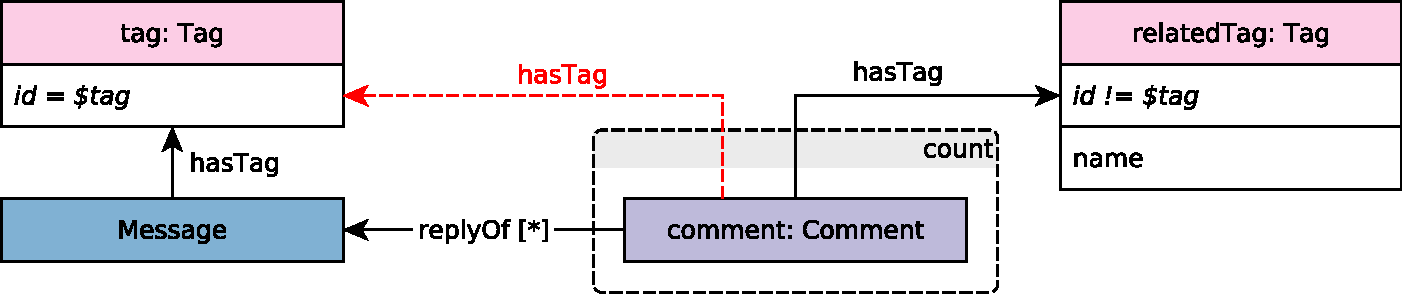
\includegraphics[scale=\patternscale,margin=0cm .2cm]{patterns/bi08}\hfill\vadjust{} \\ \hline
%
	description & Find all Messages that have a given Tag. Find the related Tags attached
to replies of these Messages (TODO - transitive? szarnyasg), but only of
those replies that do not have the given Tag.

Group the Tags by name, and get the count of replies in each group.
 \\ \hline
	
%
	group by       &
	\multicolumn{1}{>{\raggedright}X|}{
		\varname{relatedTag.name}
		} \\ \hline
	
%
	parameters  &
	\vspace{1.1ex}{\begin{tabularx}{14.2cm}{|c|M|m{2cm}|Y|} \hline
	\cellcolor{black!70} \color{white} $\mathsf{1}$ & \varname{tag} & \cellcolor{gray!20} \vartype{32-bit Integer} &  \\ \hline
	\end{tabularx}}\vspace{1.1ex} \\ \hline
%
	result      &
	\vspace{1.1ex}{\begin{tabularx}{14.2cm}{|c|M|m{2cm}|Y|} \hline
	\cellcolor{black!70} \color{white} $\mathsf{1}$ & \varname{relatedTag.name} & \cellcolor{gray!20} \vartype{String} &  \\ \hline
	\cellcolor{black!70} \color{white} $\mathsf{2}$ & \varname{count} & \cellcolor{gray!20} \vartype{32-bit Integer} &  \\ \hline
	\end{tabularx}}\vspace{1.1ex} \\ \hline
	%
	sort        &
	\vspace{1.1ex}{\begin{tabular}{|c|l|c|} \hline
	\cellcolor{black!70} \color{white} $\mathsf{1}$ & \varname{count} & \cellcolor{gray!20} $\desc$ \\ \hline
	\cellcolor{black!70} \color{white} $\mathsf{2}$ & \varname{relatedTag.name} & \cellcolor{gray!20} $\asc$ \\ \hline
	\end{tabular}}\vspace{1.1ex} \\ \hline
	%
	limit       & 100 \\ \hline
	%
	choke points &
	\multicolumn{1}{>{\raggedright}X|}{
		\chokepoint{1.6}, 
		\chokepoint{3.3}, 
		\chokepoint{5.2}
		}\\ \hline
\end{tabularx}
\clearpage
\renewcommand*{\arraystretch}{1.1}

\noindent\begin{tabularx}{17cm}{|p{1.95cm}|X|}
	\hline
	number      & 9                                                          \\ \hline
%
	title       & Forum with related Tags                                                           \\ \hline
	\multicolumn{2}{|c|}{ 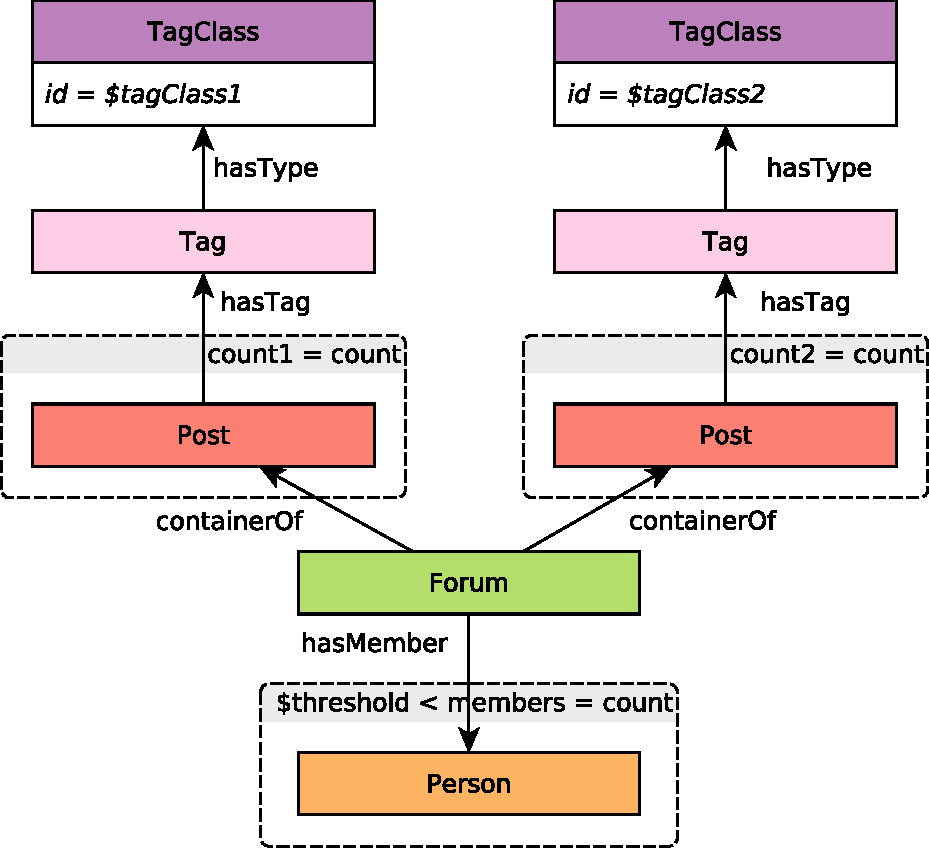
\includegraphics[scale=\patternscale,margin=0cm .2cm]{patterns/q09}} \\ \hline
	description & Given two TagClasses (\texttt{tagClass1} \& \texttt{tagClass2}), find
Forums that contain at least one Post with a Tag from \texttt{tagClass1}
and at least one Post with a Tag from \texttt{tagClass2} (direct
children not transitive) -- this may be the same Post.

Consider the Forums with a number of members greater than a given
threshold. For every such forum, count the number of Posts that have a
Tag from TagClass1 (count1), and the number of posts that have a tag
from TagClass2.
 \\ \hline
	
%
	parameters  &
	\vspace{1.1ex}{\begin{tabularx}{14.38cm}{|c|M|m{2cm}|Y} \hline
	\cellcolor{black!70} \color{white} $\mathsf{1}$ & \varname{tagClass1} & \cellcolor{gray!20} \vartype{32-bit Integer} &  \\\hline
	\cellcolor{black!70} \color{white} $\mathsf{2}$ & \varname{tagClass2} & \cellcolor{gray!20} \vartype{32-bit Integer} &  \\\hline
	\cellcolor{black!70} \color{white} $\mathsf{3}$ & \varname{threshold} & \cellcolor{gray!20} \vartype{32-bit Integer} &  \\
	\end{tabularx}} \\ \hline
%
	result      &
	\vspace{1.1ex}{\begin{tabularx}{14.38cm}{|c|M|m{2cm}|Y} \hline
	\cellcolor{black!70} \color{white} $\mathsf{1}$ & \varname{forum.id} & \cellcolor{gray!20} \vartype{64-bit Integer} &  \\\hline
	\cellcolor{black!70} \color{white} $\mathsf{2}$ & \varname{count1} & \cellcolor{gray!20} \vartype{32-bit Integer} & Number of Posts with at least one tag belonging to tagClass1 \\\hline
	\cellcolor{black!70} \color{white} $\mathsf{3}$ & \varname{count2} & \cellcolor{gray!20} \vartype{32-bit Integer} & Number of Posts with at least one tag belonging to tagClass2 \\
	\end{tabularx}} \\ \hline
	%
	sort        &
	\vspace{1.1ex}{\begin{tabular}{|c|l|c|} \hline
	\cellcolor{black!70} \color{white} $\mathsf{1}$ & \varname{count2} & \cellcolor{gray!20} $\desc$ \\\hline
	\cellcolor{black!70} \color{white} $\mathsf{2}$ & \varname{count1} & \cellcolor{gray!20} $\desc$ \\\hline
	\cellcolor{black!70} \color{white} $\mathsf{3}$ & \varname{forum.id} & \cellcolor{gray!20} $\asc$ \\
	\end{tabular}} \\ \hline
	%
	limit       & 100 \\ \hline
	%
	choke points &
	\multicolumn{1}{>{\raggedright}X|}{
		\chokepoint{1.2}, 
		\chokepoint{1.4}, 
		\chokepoint{2.1}, 
		\chokepoint{2.3}, 
		\chokepoint{2.4}
		}\\ \hline
\end{tabularx}
\clearpage
\renewcommand*{\arraystretch}{1.1}

\noindent\begin{tabularx}{17cm}{|p{1.95cm}|X|}
	\hline
	number      & 10                                                          \\ \hline
%
	title       & Central Person for a Tag                                                           \\ \hline
	\multicolumn{2}{|c|}{ 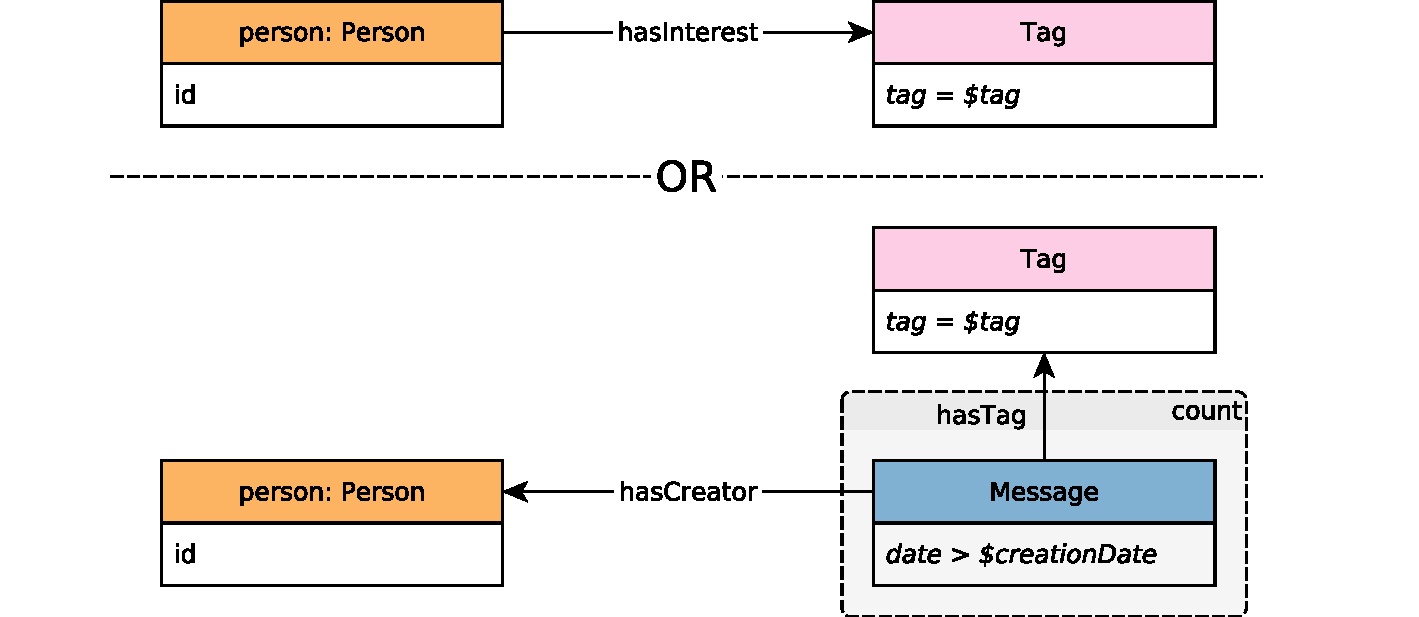
\includegraphics[scale=\patternscale,margin=0cm .2cm]{patterns/q10}} \\ \hline
	description & Given a Tag, find all Persons that are either interested in the Tag, or
have written a Message (Post or Comment) with creation date after a
given date and that has a given Tag. For each Person, compute the score
as the sum of the following two aspects:

\begin{itemize}
\tightlist
\item
  100, if the Person has this tag as their interest, or 0 otherwise
\item
  number of messages by this person with the given tag
\end{itemize}
 \\ \hline
	
%
	parameters  &
	\vspace{1.1ex}{\begin{tabularx}{14.2cm}{|c|l|m{2cm}|Y|} \hline
	\cellcolor{black!70} \color{white} $\mathsf{1}$ & \varname{tag} & \cellcolor{gray!20} \vartype{32-bit Integer} &  \\\hline
	\cellcolor{black!70} \color{white} $\mathsf{2}$ & \varname{date} & \cellcolor{gray!20} \vartype{Date} &  \\
	\end{tabularx}} \\ \hline
%
	result      &
	\vspace{1.1ex}{\begin{tabularx}{14.2cm}{|c|l|m{2cm}|Y|} \hline
	\cellcolor{black!70} \color{white} $\mathsf{1}$ & \varname{person.id} & \cellcolor{gray!20} \vartype{64-bit Integer} &  \\\hline
	\cellcolor{black!70} \color{white} $\mathsf{2}$ & \varname{score} & \cellcolor{gray!20} \vartype{32-bit Integer} &  \\\hline
	\cellcolor{black!70} \color{white} $\mathsf{3}$ & \varname{friendsScore} & \cellcolor{gray!20} \vartype{32-bit Integer} & The sum of the score of the Person's friends \\
	\end{tabularx}} \\ \hline
	%
	sort        &
	\vspace{1.1ex}{\begin{tabular}{|c|l|c|} \hline
	\cellcolor{black!70} \color{white} $\mathsf{1}$ & \varname{score + friendsScore} & \cellcolor{gray!20} $\desc$ \\\hline
	\cellcolor{black!70} \color{white} $\mathsf{2}$ & \varname{person.id} & \cellcolor{gray!20} $\asc$ \\
	\end{tabular}} \\ \hline
	%
	limit       & 100 \\ \hline
	%
	choke points &
	\multicolumn{1}{>{\raggedright}X|}{
		\chokepoint{1.2}, 
		\chokepoint{2.1}, 
		\chokepoint{2.3}, 
		\chokepoint{3.2}
		}\\ \hline
\end{tabularx}
\clearpage
\renewcommand*{\arraystretch}{1.5}
\begin{tabularx}{15cm}{|p{2.1cm}@{\hskip 1ex}|@{\hskip 1ex}X|}
	\hline
	number      & 11                                                          \\ \hline
	title       & Unrelated replies                                                           \\ \hline
	\multicolumn{2}{|c|}{ 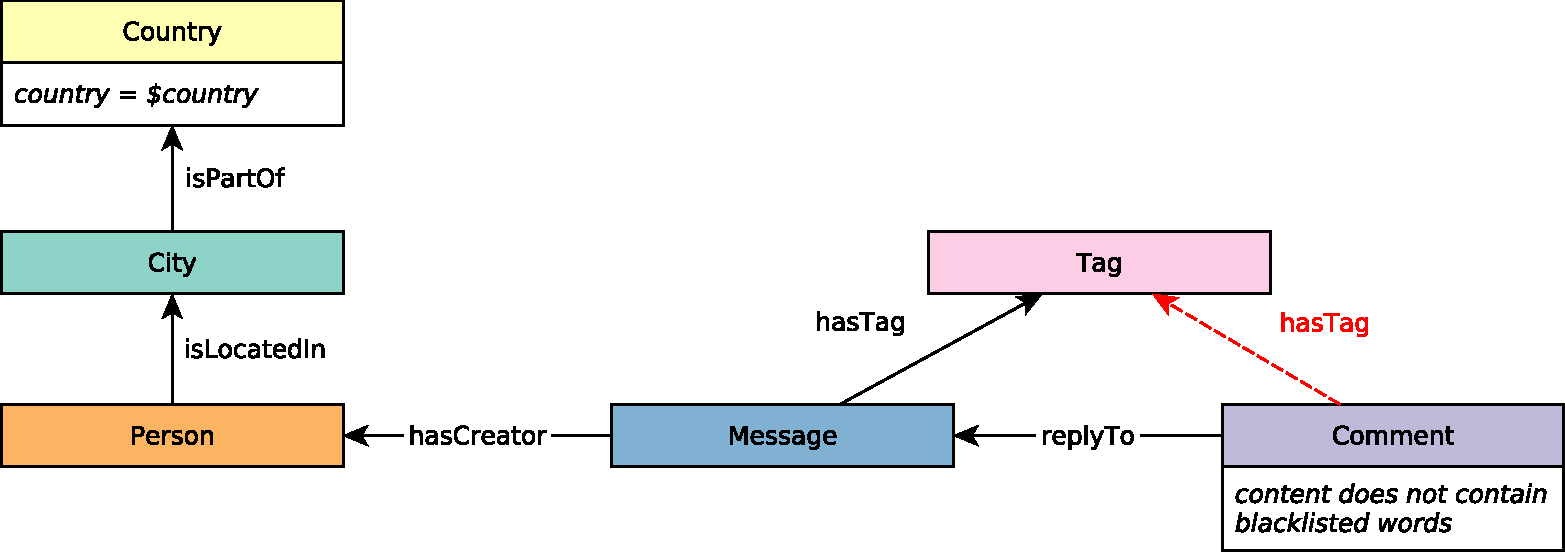
\includegraphics[scale=\patternscale,margin=0cm .2cm]{patterns/q11}} \\ \hline
	description & Find those Persons of a given country that replied to any Message, such
that the reply does not have any Tag in common with the Message {[}are
transitive replies considered or not? - SzG{]}. Consider only those
replies not containing any word from a given blacklist. For each Person
and valid reply, retrieve the Tags associated with the reply, and
retrieve the number of likes on the reply.
 \\ \hline
	
	group       &
	\multicolumn{1}{>{\raggedright}X|}{
		\varname{person.id}, 
		\varname{tag.name}
		}\\ \hline
	
	parameters  &
	\multicolumn{1}{>{\raggedright}X|}{
		\variable{country}{32bitInteger} \\
		\variable{blacklist}{String[]} 
		}\\ \hline
	result      &
	\multicolumn{1}{>{\raggedright}X|}{
		\variable{person.id}{64bitInteger}\\
		\variable{tag.name}{String}\\
		\variable{countLikes}{32bitInteger}The count of Likes to replies with that Tag.\\
		\variable{countReplies}{32bitInteger}The count of replies with that Tag.
		}\\ \hline
	sort        &
	\multicolumn{1}{>{\raggedright}X|}{
		\sortentry{countLikes}{\desc}\\
		\sortentry{person.id}{\asc}\\
		\sortentry{tag.name}{\asc}
		}\\ \hline
	limit       & 100                                                           \\ \hline
	choke points        &
	\multicolumn{1}{>{\raggedright}X|}{
		\chokepoint{1.1}, 
		\chokepoint{2.1}, 
		\chokepoint{2.2}, 
		\chokepoint{2.3}, 
		\chokepoint{3.1}, 
		\chokepoint{3.2}, 
		\chokepoint{6.1}
		}\\ \hline
\end{tabularx}
\clearpage

\renewcommand*{\arraystretch}{1.1}

\noindent\begin{tabularx}{17cm}{|p{1.95cm}|X|}
	\hline
	workload    & BI \\ \hline
%
	query       & 12 \\ \hline
%
	title       & Trending Posts \\ \hline
	\multicolumn{2}{|c|}{ 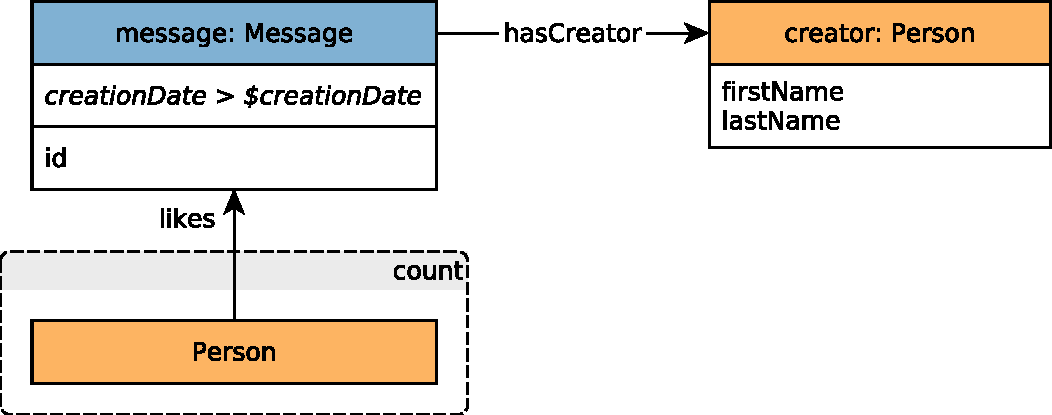
\includegraphics[scale=\patternscale,margin=0cm .2cm]{patterns/bi12}} \\ \hline
	description & Find all Messages created after a given date, that received more than a
given number of likes.
 \\ \hline
	
%
	parameters  &
	\vspace{1.1ex}{\begin{tabularx}{14.2cm}{|c|M|m{2cm}|Y|} \hline
	\cellcolor{black!70} \color{white} $\mathsf{1}$ & \varname{creationDate} & \cellcolor{gray!20} \vartype{Date} &  \\ \hline
	\cellcolor{black!70} \color{white} $\mathsf{2}$ & \varname{likeThreshold} & \cellcolor{gray!20} \vartype{32-bit Integer} &  \\ \hline
	\end{tabularx}}\vspace{1.1ex} \\ \hline
%
	result      &
	\vspace{1.1ex}{\begin{tabularx}{14.2cm}{|c|M|m{2cm}|Y|} \hline
	\cellcolor{black!70} \color{white} $\mathsf{1}$ & \varname{message.id} & \cellcolor{gray!20} \vartype{64-bit Integer} &  \\ \hline
	\cellcolor{black!70} \color{white} $\mathsf{2}$ & \varname{message.creationDate} & \cellcolor{gray!20} \vartype{DateTime} &  \\ \hline
	\cellcolor{black!70} \color{white} $\mathsf{3}$ & \varname{creator.firstName} & \cellcolor{gray!20} \vartype{String} & The first name of the post's creator \\ \hline
	\cellcolor{black!70} \color{white} $\mathsf{4}$ & \varname{creator.lastName} & \cellcolor{gray!20} \vartype{String} & The last name of the post's creator \\ \hline
	\cellcolor{black!70} \color{white} $\mathsf{5}$ & \varname{likeCount} & \cellcolor{gray!20} \vartype{32-bit Integer} & The number of Likes the Post received \\ \hline
	\end{tabularx}}\vspace{1.1ex} \\ \hline
	%
	sort        &
	\vspace{1.1ex}{\begin{tabular}{|c|l|c|} \hline
	\cellcolor{black!70} \color{white} $\mathsf{1}$ & \varname{likeCount} & \cellcolor{gray!20} $\desc$ \\ \hline
	\cellcolor{black!70} \color{white} $\mathsf{2}$ & \varname{message.id} & \cellcolor{gray!20} $\asc$ \\ \hline
	\end{tabular}}\vspace{1.1ex} \\ \hline
	%
	limit       & 100 \\ \hline
	%
	choke points &
	\multicolumn{1}{>{\raggedright}X|}{
		\chokepoint{1.2}, 
		\chokepoint{2.2}, 
		\chokepoint{3.1}, 
		\chokepoint{6.1}
		}\\ \hline
\end{tabularx}
\clearpage
\renewcommand*{\arraystretch}{1.1}

\noindent\begin{tabularx}{17cm}{|p{1.95cm}|X|}
	\hline
	workload    & BI \\ \hline
%
	query       & 13 \\ \hline
%
	title       & Popular Tags per month in a country \\ \hline
%
    pattern     & \hfill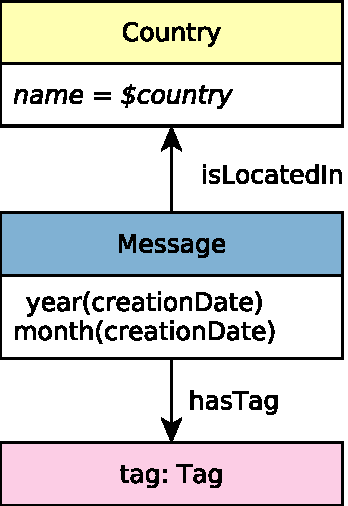
\includegraphics[scale=\patternscale,margin=0cm .2cm]{patterns/bi13}\hfill\vadjust{} \\ \hline
%
	description & Find all Messages in a given Country, as well as their Tags.

For each group, find the 5 most popular Tags, where popularity is the
number of Messages (from within the same group) where the Tag appears.
 \\ \hline
	
%
	group by       &
	\multicolumn{1}{>{\raggedright}X|}{
		\varname{year}, 
		\varname{month}
		} \\ \hline
	
%
	parameters  &
	\vspace{1.1ex}{\begin{tabularx}{14.2cm}{|c|M|m{2cm}|Y|} \hline
	\cellcolor{black!70} \color{white} $\mathsf{1}$ & \varname{country} & \cellcolor{gray!20} \vartype{String} &  \\ \hline
	\end{tabularx}}\vspace{1.1ex} \\ \hline
%
	result      &
	\vspace{1.1ex}{\begin{tabularx}{14.2cm}{|c|M|m{2cm}|Y|} \hline
	\cellcolor{black!70} \color{white} $\mathsf{1}$ & \varname{year} & \cellcolor{gray!20} \vartype{32-bit Integer} & year(message.creationDate) \\ \hline
	\cellcolor{black!70} \color{white} $\mathsf{2}$ & \varname{month} & \cellcolor{gray!20} \vartype{32-bit Integer} & month(message.creationDate) \\ \hline
	\cellcolor{black!70} \color{white} $\mathsf{3}$ & \varname{popularTags} & \cellcolor{gray!20} \vartype{TagPairs} & (tag.name - String, popularity - 32-bit Integer), sorted descending by popularity, then ascending by tag name \\ \hline
	\end{tabularx}}\vspace{1.1ex} \\ \hline
	%
	sort        &
	\vspace{1.1ex}{\begin{tabular}{|c|l|c|} \hline
	\cellcolor{black!70} \color{white} $\mathsf{1}$ & \varname{year} & \cellcolor{gray!20} $\desc$ \\ \hline
	\cellcolor{black!70} \color{white} $\mathsf{2}$ & \varname{month} & \cellcolor{gray!20} $\asc$ \\ \hline
	\end{tabular}}\vspace{1.1ex} \\ \hline
	%
	limit       & 100 \\ \hline
	%
	choke points &
	\multicolumn{1}{>{\raggedright}X|}{
		\chokepoint{1.2}, 
		\chokepoint{2.2}, 
		\chokepoint{2.3}, 
		\chokepoint{3.2}, 
		\chokepoint{6.1}
		}\\ \hline
\end{tabularx}
\clearpage
\renewcommand*{\arraystretch}{1.1}

\noindent\begin{tabularx}{17cm}{|p{1.95cm}|X|}
	\hline
	number      & 14                                                          \\ \hline
%
	title       & Top thread initiators                                                           \\ \hline
	\multicolumn{2}{|c|}{ 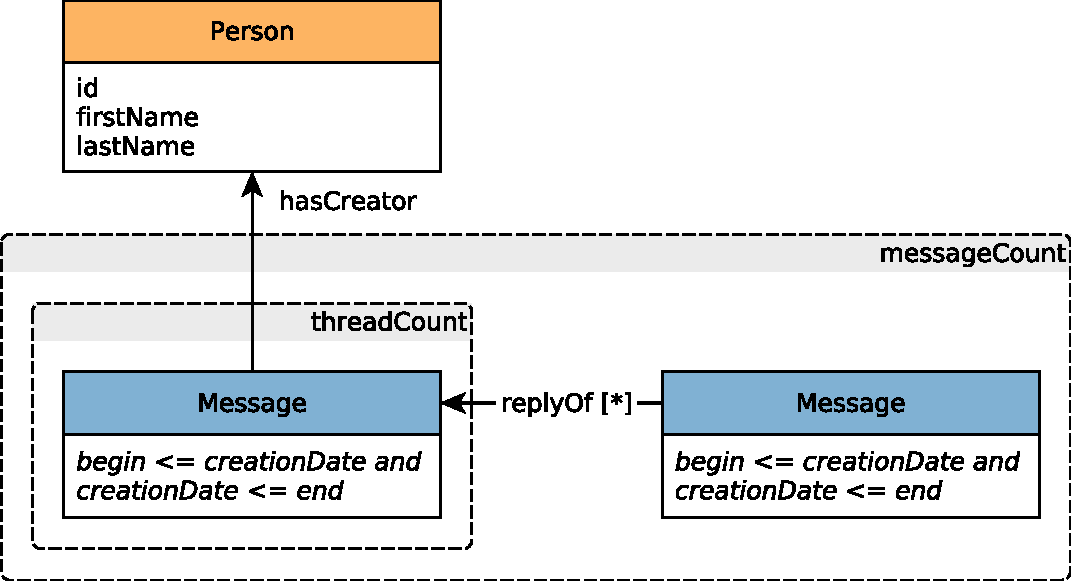
\includegraphics[scale=\patternscale,margin=0cm .2cm]{patterns/q14}} \\ \hline
	description & For each person, count the number Posts they created in the time
interval \texttt{(begin,\ end)}, and the number of messages in each of
their (transitive) reply trees. When calculating message counts only
consider messages created within the given time interval.

Return each person, number of Posts they created, and the count of all
messages that appeared in the reply trees (including Post at tree root)
they created.
 \\ \hline
	
%
	parameters  &
	\vspace{1.1ex}{\begin{tabularx}{14.38cm}{|c|M|m{2cm}|Y} \hline
	\cellcolor{black!70} \color{white} $\mathsf{1}$ & \varname{begin} & \cellcolor{gray!20} \vartype{Date} &  \\\hline
	\cellcolor{black!70} \color{white} $\mathsf{2}$ & \varname{end} & \cellcolor{gray!20} \vartype{Date} &  \\
	\end{tabularx}} \\ \hline
%
	result      &
	\vspace{1.1ex}{\begin{tabularx}{14.38cm}{|c|M|m{2cm}|Y} \hline
	\cellcolor{black!70} \color{white} $\mathsf{1}$ & \varname{person.id} & \cellcolor{gray!20} \vartype{64-bit Integer} &  \\\hline
	\cellcolor{black!70} \color{white} $\mathsf{2}$ & \varname{person.firstName} & \cellcolor{gray!20} \vartype{String} &  \\\hline
	\cellcolor{black!70} \color{white} $\mathsf{3}$ & \varname{person.lastName} & \cellcolor{gray!20} \vartype{String} &  \\\hline
	\cellcolor{black!70} \color{white} $\mathsf{4}$ & \varname{threadCount} & \cellcolor{gray!20} \vartype{32-bit Integer} & The number of threads initiated by that Person \\\hline
	\cellcolor{black!70} \color{white} $\mathsf{5}$ & \varname{messageCount} & \cellcolor{gray!20} \vartype{32-bit Integer} & The number of messages created in all the threads this Person initiated \\
	\end{tabularx}} \\ \hline
	%
	sort        &
	\vspace{1.1ex}{\begin{tabular}{|c|l|c|} \hline
	\cellcolor{black!70} \color{white} $\mathsf{1}$ & \varname{messageCount} & \cellcolor{gray!20} $\desc$ \\\hline
	\cellcolor{black!70} \color{white} $\mathsf{2}$ & \varname{person.id} & \cellcolor{gray!20} $\asc$ \\
	\end{tabular}} \\ \hline
	%
	limit       & 100 \\ \hline
	%
	choke points &
	\multicolumn{1}{>{\raggedright}X|}{
		\chokepoint{1.2}, 
		\chokepoint{2.2}, 
		\chokepoint{2.3}, 
		\chokepoint{3.2}, 
		\chokepoint{7.2}, 
		\chokepoint{7.3}, 
		\chokepoint{7.4}
		}\\ \hline
\end{tabularx}
\clearpage
\renewcommand*{\arraystretch}{1.1}

\noindent\begin{tabularx}{17cm}{|p{1.95cm}|X|}
	\hline
	workload    & bi \\ \hline
%
	query       & 15 \\ \hline
%
	title       & Social normals \\ \hline
	\multicolumn{2}{|c|}{ 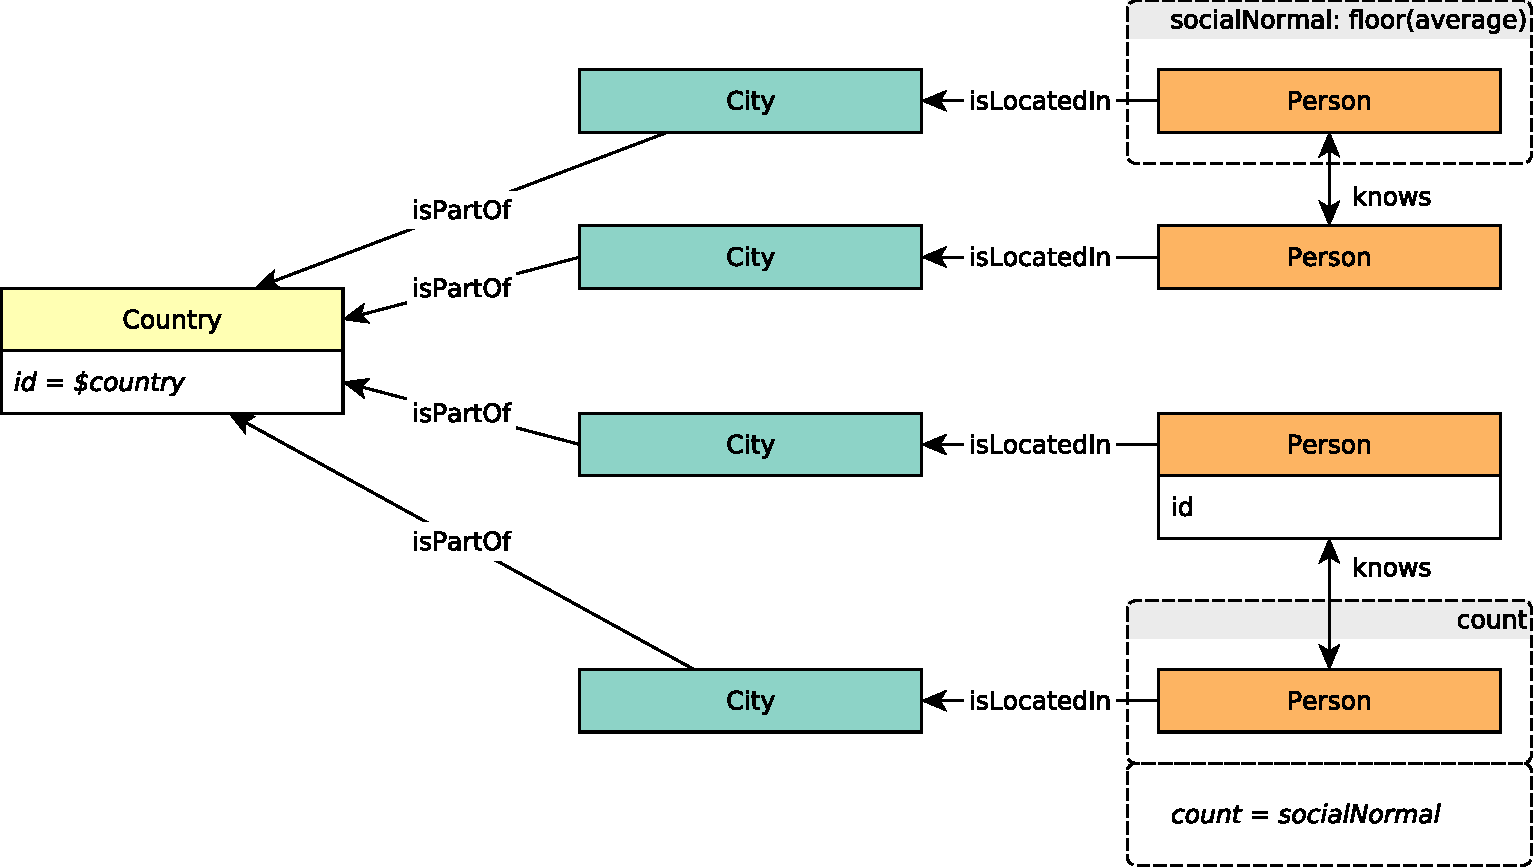
\includegraphics[scale=\patternscale,margin=0cm .2cm]{patterns/bi15}} \\ \hline
	description & Given a country, find all Persons of the country whose number of friends
in the given country equals the (floor of) average number of friends
that Persons of the given country have in the given country.
 \\ \hline
	
%
	parameters  &
	\vspace{1.1ex}{\begin{tabularx}{14.38cm}{|c|M|m{2cm}|Y} \hline
	\cellcolor{black!70} \color{white} $\mathsf{1}$ & \varname{country} & \cellcolor{gray!20} \vartype{32-bit Integer} &  \\
	\end{tabularx}} \\ \hline
%
	result      &
	\vspace{1.1ex}{\begin{tabularx}{14.38cm}{|c|M|m{2cm}|Y} \hline
	\cellcolor{black!70} \color{white} $\mathsf{1}$ & \varname{person.id} & \cellcolor{gray!20} \vartype{64-bit Integer} &  \\\hline
	\cellcolor{black!70} \color{white} $\mathsf{2}$ & \varname{count} & \cellcolor{gray!20} \vartype{32-bit Integer} &  \\
	\end{tabularx}} \\ \hline
	%
	sort        &
	\vspace{1.1ex}{\begin{tabular}{|c|l|c|} \hline
	\cellcolor{black!70} \color{white} $\mathsf{1}$ & \varname{person.id} & \cellcolor{gray!20} $\asc$ \\
	\end{tabular}} \\ \hline
	%
	limit       & 100 \\ \hline
	%
	choke points &
	\multicolumn{1}{>{\raggedright}X|}{
		\chokepoint{1.2}, 
		\chokepoint{2.3}, 
		\chokepoint{3.2}, 
		\chokepoint{3.3}, 
		\chokepoint{5.3}, 
		\chokepoint{6.1}
		}\\ \hline
\end{tabularx}
\clearpage
\renewcommand*{\arraystretch}{1.1}

\noindent\begin{tabularx}{17cm}{|p{1.95cm}|X|}
	\hline
	workload    & BI \\ \hline
%
	query       & 16 \\ \hline
%
	title       & Experts in social circle \\ \hline
	\multicolumn{2}{|c|}{ 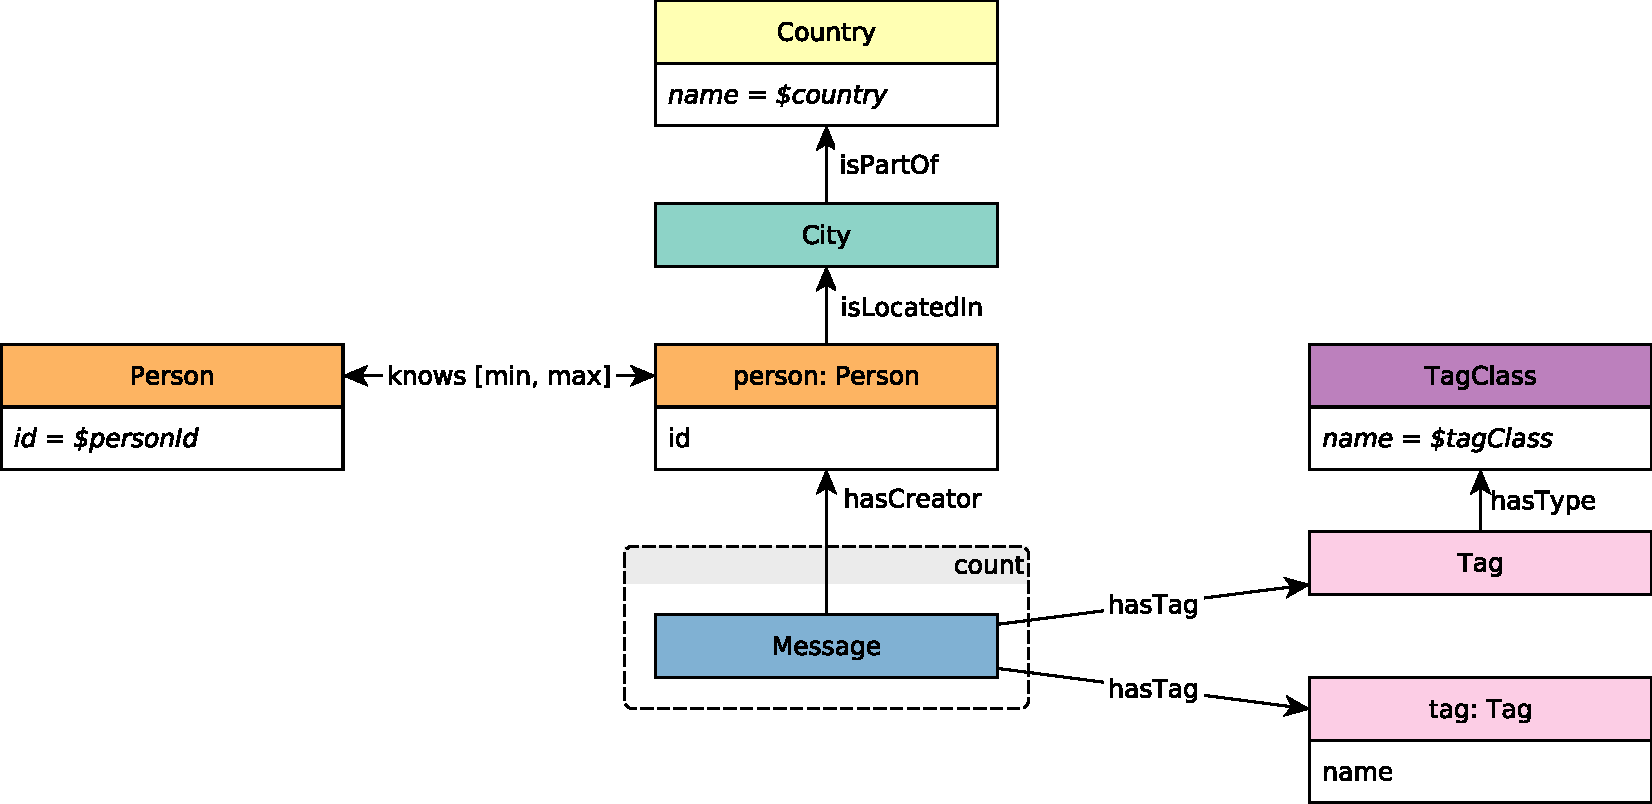
\includegraphics[scale=\patternscale,margin=0cm .2cm]{patterns/bi16}} \\ \hline
	description & Given a Person, find all other Persons that live in a given country and
are connected to given person by a transitive path with length in range
\texttt{{[}min,\ max{]}} through the knows relation.

{[}DISCUSS: edge isomorphism semantics{]}

For each of these Persons, retrieve all of their Messages (Posts \&
Comments) that contain at least one Tag belonging to a given TagClass
(direct relation not transitive).

For each Message, also retrieve its Tags.

TODO {[}szarnyasg{]}: what is postCount?
 \\ \hline
	
%
	group by       &
	\multicolumn{1}{>{\raggedright}X|}{
		\varname{tag.name}, 
		\varname{person.id}
		} \\ \hline
	
%
	parameters  &
	\vspace{1.1ex}{\begin{tabularx}{14.38cm}{|c|M|m{2cm}|Y} \hline
	\cellcolor{black!70} \color{white} $\mathsf{1}$ & \varname{personId} & \cellcolor{gray!20} \vartype{64-bit Integer} &  \\\hline
	\cellcolor{black!70} \color{white} $\mathsf{2}$ & \varname{country} & \cellcolor{gray!20} \vartype{String} &  \\\hline
	\cellcolor{black!70} \color{white} $\mathsf{3}$ & \varname{tagClass} & \cellcolor{gray!20} \vartype{String} &  \\\hline
	\cellcolor{black!70} \color{white} $\mathsf{4}$ & \varname{minPathDistance} & \cellcolor{gray!20} \vartype{32-bit Integer} &  \\\hline
	\cellcolor{black!70} \color{white} $\mathsf{5}$ & \varname{maxPathDistance} & \cellcolor{gray!20} \vartype{32-bit Integer} &  \\
	\end{tabularx}} \\ \hline
%
	result      &
	\vspace{1.1ex}{\begin{tabularx}{14.38cm}{|c|M|m{2cm}|Y} \hline
	\cellcolor{black!70} \color{white} $\mathsf{1}$ & \varname{person.id} & \cellcolor{gray!20} \vartype{64-bit Integer} &  \\\hline
	\cellcolor{black!70} \color{white} $\mathsf{2}$ & \varname{tag.name} & \cellcolor{gray!20} \vartype{String} &  \\\hline
	\cellcolor{black!70} \color{white} $\mathsf{3}$ & \varname{messageCount} & \cellcolor{gray!20} \vartype{32-bit Integer} & number of Messages created by that Person containing that Tag \\
	\end{tabularx}} \\ \hline
	%
	sort        &
	\vspace{1.1ex}{\begin{tabular}{|c|l|c|} \hline
	\cellcolor{black!70} \color{white} $\mathsf{1}$ & \varname{messageCount} & \cellcolor{gray!20} $\desc$ \\\hline
	\cellcolor{black!70} \color{white} $\mathsf{2}$ & \varname{tag.name} & \cellcolor{gray!20} $\asc$ \\\hline
	\cellcolor{black!70} \color{white} $\mathsf{3}$ & \varname{person.id} & \cellcolor{gray!20} $\asc$ \\
	\end{tabular}} \\ \hline
	%
	limit       & 100 \\ \hline
	%
	choke points &
	\multicolumn{1}{>{\raggedright}X|}{
		\chokepoint{1.2}, 
		\chokepoint{1.4}, 
		\chokepoint{2.3}, 
		\chokepoint{2.4}, 
		\chokepoint{3.3}, 
		\chokepoint{7.2}, 
		\chokepoint{7.3}
		}\\ \hline
\end{tabularx}
\clearpage
\renewcommand*{\arraystretch}{1.5}
\noindent\begin{tabularx}{17cm}{|p{1.95cm}|X|}
	\hline
	number      & 17                                                          \\ \hline
	title       & Friend triangles                                                           \\ \hline
	\multicolumn{2}{|c|}{ 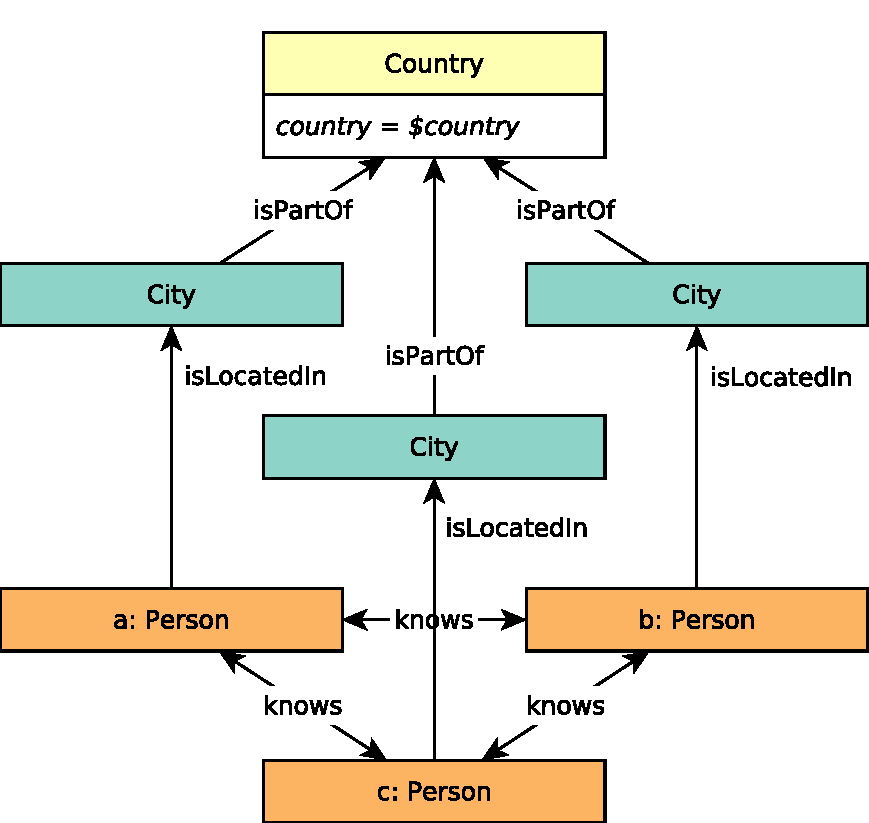
\includegraphics[scale=\patternscale,margin=0cm .2cm]{patterns/q17}} \\ \hline
	description & For a given country, count all the distinct triples of persons such that
\texttt{a} is friend of \texttt{b}, \texttt{b} is friend of \texttt{c},
and \texttt{c} is friend of \texttt{a}.

Distinct means that given a triple \emph{t1} in the result set \emph{R}
of all qualified triples, there is not a triple \emph{t2} in \emph{R}
such that \textbar{}\emph{t1} U \emph{b}\textbar{} = 3.
 \\ \hline
	
	parameters  &
	\renewcommand*{\arraystretch}{1.0}
	\vspace{-1.8ex}{\begin{tabularx}{14.2cm}{|c|l|p{2cm}|Y|} \hline
	\cellcolor{black!70} \color{white} $\mathsf{ 1 }$ & \varname{country} & \cellcolor{gray!20} \vartype{String} & \\ 
	\end{tabularx}} \\ \hline
	result      &
	\renewcommand*{\arraystretch}{1.0}
	\vspace{-1.8ex}{\begin{tabularx}{14.2cm}{|c|l|p{2cm}|Y|} \hline
	\cellcolor{black!70} \color{white} $\mathsf{ 1 }$ & \varname{count} & \cellcolor{gray!20} \vartype{32bitInteger} & \\ 
	\end{tabularx}} \\ \hline
	choke points        &
	\multicolumn{1}{>{\raggedright}X|}{
		\chokepoint{1.1}, 
		\chokepoint{2.3}
		}\\ \hline
\end{tabularx}
\clearpage
\renewcommand*{\arraystretch}{1.5}
\begin{tabularx}{15cm}{|p{2.1cm}@{\hskip 1ex}|@{\hskip 1ex}X|}
	\hline
	number      & 18                                                          \\ \hline
	title       & How many persons have a given number of posts                                                           \\ \hline
	\multicolumn{2}{|c|}{ \includegraphics[scale=\patternscale,margin=0cm .2cm]{patterns/q18}} \\ \hline
	description & For each Person, count the number of Messages (Posts \& Comments) they
made.

Only consider messages with:

\begin{itemize}
\tightlist
\item
  length below the \texttt{lengthThreshold}
\item
  creationDate after \texttt{creationDate} (TODO - is after exclusive or
  inclusive, does it allow equality?)
\item
  any of the given \texttt{languages} (TODO - only Posts have a
  language, messages do not)
\end{itemize}
 \\ \hline
	
	group       &
	\multicolumn{1}{>{\raggedright}X|}{
		\varname{messageCount}
		}\\ \hline
	
	parameters  &
	\multicolumn{1}{>{\raggedright}X|}{
		\variable{creationDate}{Date} \\
		\variable{lengthThreshold}{TODO (32bitInteger?)} 
		}\\ \hline
	result      &
	\multicolumn{1}{>{\raggedright}X|}{
		\variable{messageCount}{32bitInteger}number of messages created\\
		\variable{personCount}{32bitInteger}the number of Persons with `messageCount` messages
		}\\ \hline
	sort        &
	\multicolumn{1}{>{\raggedright}X|}{
		\sortentry{personCount}{\desc}
		}\\ \hline
	choke points        &
	\multicolumn{1}{>{\raggedright}X|}{
		\chokepoint{1.1}, 
		\chokepoint{1.2}, 
		\chokepoint{1.6}, 
		\chokepoint{3.2}, 
		\chokepoint{4.2}, 
		\chokepoint{4.3}
		}\\ \hline
\end{tabularx}
\clearpage

\renewcommand*{\arraystretch}{1.1}

\noindent\begin{tabularx}{17cm}{|p{1.95cm}|X|}
	\hline
	workload    & BI \\ \hline
%
	query       & 19 \\ \hline
%
	title       & Stranger's interaction \\ \hline
%
    pattern     & \hfill\includegraphics[scale=\patternscale,margin=0cm .2cm]{patterns/bi19}\hfill\vadjust{} \\ \hline
%
	description & For all the Persons born after a certain date, find all the strangers
they interacted with, where strangers are Persons that do not Know each
other. There is no restriction on the date that strangers were born.

Consider only strangers that are members of Forums tagged with tagClass1
(direct children not transitive) AND members of Forums tagged with
tagClass2 (direct children not transitive). It does not matter if these
Tags are attached to the same Forum, or different Forums.

We define interaction as follows: a Person replies to a Message (Post or
Comment) by another Person.

For each Person, count the number of strangers they interacted
(directed) with and total number of times they interacted (directed)
with them.
 \\ \hline
	
%
	parameters  &
	\vspace{1.1ex}{\begin{tabularx}{14.2cm}{|c|M|m{2cm}|Y|} \hline
	\cellcolor{black!70} \color{white} $\mathsf{1}$ & \varname{date} & \cellcolor{gray!20} \vartype{Date} &  \\ \hline
	\cellcolor{black!70} \color{white} $\mathsf{2}$ & \varname{tagClass1} & \cellcolor{gray!20} \vartype{32-bit Integer} &  \\ \hline
	\cellcolor{black!70} \color{white} $\mathsf{3}$ & \varname{tagClass2} & \cellcolor{gray!20} \vartype{32-bit Integer} &  \\ \hline
	\end{tabularx}}\vspace{1.1ex} \\ \hline
%
	result      &
	\vspace{1.1ex}{\begin{tabularx}{14.2cm}{|c|M|m{2cm}|Y|} \hline
	\cellcolor{black!70} \color{white} $\mathsf{1}$ & \varname{person.id} & \cellcolor{gray!20} \vartype{64-bit Integer} &  \\ \hline
	\cellcolor{black!70} \color{white} $\mathsf{2}$ & \varname{strangersCount} & \cellcolor{gray!20} \vartype{32-bit Integer} &  \\ \hline
	\cellcolor{black!70} \color{white} $\mathsf{3}$ & \varname{interactionCount} & \cellcolor{gray!20} \vartype{32-bit Integer} &  \\ \hline
	\end{tabularx}}\vspace{1.1ex} \\ \hline
	%
	sort        &
	\vspace{1.1ex}{\begin{tabular}{|c|l|c|} \hline
	\cellcolor{black!70} \color{white} $\mathsf{1}$ & \varname{interactionCount} & \cellcolor{gray!20} $\desc$ \\ \hline
	\cellcolor{black!70} \color{white} $\mathsf{2}$ & \varname{person.id} & \cellcolor{gray!20} $\asc$ \\ \hline
	\end{tabular}}\vspace{1.1ex} \\ \hline
	%
	limit       & 100 \\ \hline
	%
	choke points &
	\multicolumn{1}{>{\raggedright}X|}{
		\chokepoint{1.1}, 
		\chokepoint{1.4}, 
		\chokepoint{2.1}, 
		\chokepoint{2.3}, 
		\chokepoint{2.4}, 
		\chokepoint{3.3}, 
		\chokepoint{5.1}, 
		\chokepoint{7.3}, 
		\chokepoint{7.4}
		}\\ \hline
\end{tabularx}
\clearpage
\renewcommand*{\arraystretch}{1.1}

\noindent\begin{tabularx}{17cm}{|p{1.95cm}|X|}
	\hline
	number      & 20                                                          \\ \hline
%
	title       & High-level topics                                                           \\ \hline
	\multicolumn{2}{|c|}{ \includegraphics[scale=\patternscale,margin=0cm .2cm]{patterns/q20}} \\ \hline
	description & For all given TagClasses, count number of Messages that have a Tag that
belongs to that TagClass or any of its children (all descendants through
a transitive relation).
 \\ \hline
	
%
	parameters  &
	\vspace{1.1ex}{\begin{tabularx}{14.38cm}{|c|M|m{2cm}|Y} \hline
	\cellcolor{black!70} \color{white} $\mathsf{1}$ & \varname{tagClasses} & \cellcolor{gray!20} \vartype{String[]} &  \\
	\end{tabularx}} \\ \hline
%
	result      &
	\vspace{1.1ex}{\begin{tabularx}{14.38cm}{|c|M|m{2cm}|Y} \hline
	\cellcolor{black!70} \color{white} $\mathsf{1}$ & \varname{tagClass.name} & \cellcolor{gray!20} \vartype{String} & the TagClass of the root \\\hline
	\cellcolor{black!70} \color{white} $\mathsf{2}$ & \varname{postCount} & \cellcolor{gray!20} \vartype{32-bit Integer} &  \\
	\end{tabularx}} \\ \hline
	%
	sort        &
	\vspace{1.1ex}{\begin{tabular}{|c|l|c|} \hline
	\cellcolor{black!70} \color{white} $\mathsf{1}$ & \varname{postCount} & \cellcolor{gray!20} $\desc$ \\\hline
	\cellcolor{black!70} \color{white} $\mathsf{2}$ & \varname{tagClass.name} & \cellcolor{gray!20} $\asc$ \\
	\end{tabular}} \\ \hline
	%
	limit       & 100 \\ \hline
	%
	choke points &
	\multicolumn{1}{>{\raggedright}X|}{
		\chokepoint{1.6}, 
		\chokepoint{2.1}, 
		\chokepoint{6.1}
		}\\ \hline
\end{tabularx}
\clearpage
\renewcommand*{\arraystretch}{1.1}

\noindent\begin{tabularx}{17cm}{|p{1.95cm}|X|}
	\hline
	number      & 21                                                          \\ \hline
%
	title       & Zombies in a country                                                           \\ \hline
	\multicolumn{2}{|c|}{ \includegraphics[scale=\patternscale,margin=0cm .2cm]{patterns/q21}} \\ \hline
	description & Find zombies within the given country, and return their zombie scores.

A zombie is a Person created before the given \texttt{endDate} and that
has created between \texttt{{[}0,\ 1)} Messages per month, on average,
during the time range between profile creation date and the given
\texttt{endDate}.

The number of months spans the time range from creation date of the
profile to the \texttt{endDate} and also includes partial months.
 \\ \hline
	
%
	parameters  &
	\vspace{1.1ex}{\begin{tabularx}{14.2cm}{|c|l|m{2cm}|Y|} \hline
	\cellcolor{black!70} \color{white} $\mathsf{1}$ & \varname{country} & \cellcolor{gray!20} \vartype{String} &  \\\hline
	\cellcolor{black!70} \color{white} $\mathsf{2}$ & \varname{endDate} & \cellcolor{gray!20} \vartype{Date} &  \\
	\end{tabularx}} \\ \hline
%
	result      &
	\vspace{1.1ex}{\begin{tabularx}{14.2cm}{|c|l|m{2cm}|Y|} \hline
	\cellcolor{black!70} \color{white} $\mathsf{1}$ & \varname{person.id} & \cellcolor{gray!20} \vartype{64-bit Integer} &  \\\hline
	\cellcolor{black!70} \color{white} $\mathsf{2}$ & \varname{zombieLikeCount} & \cellcolor{gray!20} \vartype{32-bit Integer} &  \\\hline
	\cellcolor{black!70} \color{white} $\mathsf{3}$ & \varname{realLikeCount} & \cellcolor{gray!20} \vartype{32-bit Integer} &  \\\hline
	\cellcolor{black!70} \color{white} $\mathsf{4}$ & \varname{zombieScore} & \cellcolor{gray!20} \vartype{32bitFloat} & the ratio between the number of likes received from zombies (`zombieLikeCount`) and the total number of likes received on that person's messages (`realLikeCount`) -- only count likes received from profiles that were created before the given `endDate`. \\
	\end{tabularx}} \\ \hline
	%
	sort        &
	\vspace{1.1ex}{\begin{tabular}{|c|l|c|} \hline
	\cellcolor{black!70} \color{white} $\mathsf{1}$ & \varname{zombieScore} & \cellcolor{gray!20} $\desc$ \\\hline
	\cellcolor{black!70} \color{white} $\mathsf{2}$ & \varname{person.id} & \cellcolor{gray!20} $\asc$ \\
	\end{tabular}} \\ \hline
	%
	limit       & 100 \\ \hline
	%
	choke points &
	\multicolumn{1}{>{\raggedright}X|}{
		\chokepoint{1.2}, 
		\chokepoint{2.1}, 
		\chokepoint{2.3}, 
		\chokepoint{2.4}, 
		\chokepoint{3.2}, 
		\chokepoint{3.3}, 
		\chokepoint{5.1}, 
		\chokepoint{5.3}
		}\\ \hline
\end{tabularx}
\clearpage
\renewcommand*{\arraystretch}{1.1}

\noindent\begin{tabularx}{17cm}{|p{1.95cm}|X|}
	\hline
	number      & 22                                                          \\ \hline
%
	title       & International dialog                                                           \\ \hline
	\multicolumn{2}{|c|}{ \includegraphics[scale=\patternscale,margin=0cm .2cm]{patterns/q22}} \\ \hline
	description & Consider all pairs of people \texttt{(p1,\ p2)} such that one is located
in a city of Country \texttt{countryX} and the other is located in a
city of Country \texttt{countryY}.

For each city of Country \texttt{countryX}, return the highest scoring
pair.

The score of a pair is defined as the sum of the scores of the following
kinds of interaction:

\begin{itemize}
\tightlist
\item
  \texttt{p1} has created a reply Comment to at least one Comment or
  Post by \texttt{p2}: \texttt{Score\ =\ 4}
\item
  \texttt{p1} has created at least one Post or Comment that \texttt{p2}
  has created a reply Comment to: \texttt{Score\ =\ 1}
\item
  \texttt{p1} and \texttt{p2} Know each other: \texttt{Score\ =\ 15}
\item
  \texttt{p1} liked at least one Post or Comment by \texttt{p2}:
  \texttt{Score\ =\ 10}
\item
  \texttt{p1} has created at least one Post or Comment that was liked by
  \texttt{p2}: \texttt{Score\ =\ 1}
\end{itemize}

I.e., the maximum score a pair can obtain is:
\texttt{4\ +\ 1\ +\ 15\ +\ 10\ +\ 1\ =\ 31}
 \\ \hline
	
%
	parameters  &
	\vspace{1.1ex}{\begin{tabularx}{14.2cm}{|c|l|m{2cm}|Y|} \hline
	\cellcolor{black!70} \color{white} $\mathsf{1}$ & \varname{countryX} & \cellcolor{gray!20} \vartype{String} &  \\\hline
	\cellcolor{black!70} \color{white} $\mathsf{2}$ & \varname{countryY} & \cellcolor{gray!20} \vartype{String} &  \\
	\end{tabularx}} \\ \hline
%
	result      &
	\vspace{1.1ex}{\begin{tabularx}{14.2cm}{|c|l|m{2cm}|Y|} \hline
	\cellcolor{black!70} \color{white} $\mathsf{1}$ & \varname{p1.id} & \cellcolor{gray!20} \vartype{64-bit Integer} &  \\\hline
	\cellcolor{black!70} \color{white} $\mathsf{2}$ & \varname{p2.id} & \cellcolor{gray!20} \vartype{64-bit Integer} &  \\\hline
	\cellcolor{black!70} \color{white} $\mathsf{3}$ & \varname{cityX.name} & \cellcolor{gray!20} \vartype{String} &  \\\hline
	\cellcolor{black!70} \color{white} $\mathsf{4}$ & \varname{score} & \cellcolor{gray!20} \vartype{32-bit Integer} &  \\
	\end{tabularx}} \\ \hline
	%
	sort        &
	\vspace{1.1ex}{\begin{tabular}{|c|l|c|} \hline
	\cellcolor{black!70} \color{white} $\mathsf{1}$ & \varname{score} & \cellcolor{gray!20} $\desc$ \\\hline
	\cellcolor{black!70} \color{white} $\mathsf{2}$ & \varname{p1.id} & \cellcolor{gray!20} $\asc$ \\\hline
	\cellcolor{black!70} \color{white} $\mathsf{3}$ & \varname{p2.id} & \cellcolor{gray!20} $\asc$ \\
	\end{tabular}} \\ \hline
	%
	%
	choke points &
	\multicolumn{1}{>{\raggedright}X|}{
		\chokepoint{1.4}, 
		\chokepoint{1.6}, 
		\chokepoint{2.1}, 
		\chokepoint{3.1}, 
		\chokepoint{3.3}, 
		\chokepoint{5.1}, 
		\chokepoint{5.2}, 
		\chokepoint{5.3}
		}\\ \hline
\end{tabularx}
\clearpage
\renewcommand*{\arraystretch}{1.1}

\noindent\begin{tabularx}{17cm}{|p{1.95cm}|X|}
	\hline
	workload    & bi \\ \hline
%
	query       & 23 \\ \hline
%
	title       & Holiday destinations \\ \hline
	\multicolumn{2}{|c|}{ \includegraphics[scale=\patternscale,margin=0cm .2cm]{patterns/bi23}} \\ \hline
	description & Count the messages all residents of Country \texttt{country} have
written abroad grouped by month and Country. A Message was written
abroad if the Country the Message was written in is different than the
Country of the Person it was written by.
 \\ \hline
	
%
	parameters  &
	\vspace{1.1ex}{\begin{tabularx}{14.38cm}{|c|M|m{2cm}|Y} \hline
	\cellcolor{black!70} \color{white} $\mathsf{1}$ & \varname{country} & \cellcolor{gray!20} \vartype{String} &  \\
	\end{tabularx}} \\ \hline
%
	result      &
	\vspace{1.1ex}{\begin{tabularx}{14.38cm}{|c|M|m{2cm}|Y} \hline
	\cellcolor{black!70} \color{white} $\mathsf{1}$ & \varname{messageCount} & \cellcolor{gray!20} \vartype{32-bit Integer} & The number of messages in each group \\\hline
	\cellcolor{black!70} \color{white} $\mathsf{2}$ & \varname{country.name} & \cellcolor{gray!20} \vartype{String} & The name of the destination country \\\hline
	\cellcolor{black!70} \color{white} $\mathsf{3}$ & \varname{month} & \cellcolor{gray!20} \vartype{32-bit Integer} &  \\
	\end{tabularx}} \\ \hline
	%
	sort        &
	\vspace{1.1ex}{\begin{tabular}{|c|l|c|} \hline
	\cellcolor{black!70} \color{white} $\mathsf{1}$ & \varname{messageCount} & \cellcolor{gray!20} $\desc$ \\\hline
	\cellcolor{black!70} \color{white} $\mathsf{2}$ & \varname{country.name} & \cellcolor{gray!20} $\asc$ \\\hline
	\cellcolor{black!70} \color{white} $\mathsf{3}$ & \varname{month} & \cellcolor{gray!20} $\asc$ \\
	\end{tabular}} \\ \hline
	%
	limit       & 100 \\ \hline
	%
	choke points &
	\multicolumn{1}{>{\raggedright}X|}{
		\chokepoint{1.6}, 
		\chokepoint{2.3}, 
		\chokepoint{2.4}, 
		\chokepoint{3.3}, 
		\chokepoint{4.3}
		}\\ \hline
\end{tabularx}
\clearpage
\renewcommand*{\arraystretch}{1.1}

\noindent\begin{tabularx}{17cm}{|p{1.95cm}|X|}
	\hline
	workload    & bi \\ \hline
%
	query       & 24 \\ \hline
%
	title       & Messages by Topic and Continent \\ \hline
	\multicolumn{2}{|c|}{ \includegraphics[scale=\patternscale,margin=0cm .2cm]{patterns/bi24}} \\ \hline
	description & Find all Messages tagged with a Tag from the given TagClass
(non-transitive).

Count all messages and their likes grouped by continent, year, and
month. (TODO - do we group the Messages or the Persons who liked the
Messages by continent? I think the former one - szarnyasg)
 \\ \hline
	
%
	group by       &
	\multicolumn{1}{>{\raggedright}X|}{
		\varname{year}, 
		\varname{month}, 
		\varname{continent.name}
		} \\ \hline
	
%
	parameters  &
	\vspace{1.1ex}{\begin{tabularx}{14.38cm}{|c|M|m{2cm}|Y} \hline
	\cellcolor{black!70} \color{white} $\mathsf{1}$ & \varname{tagClass} & \cellcolor{gray!20} \vartype{String} &  \\
	\end{tabularx}} \\ \hline
%
	result      &
	\vspace{1.1ex}{\begin{tabularx}{14.38cm}{|c|M|m{2cm}|Y} \hline
	\cellcolor{black!70} \color{white} $\mathsf{1}$ & \varname{messageCount} & \cellcolor{gray!20} \vartype{32-bit Integer} &  \\\hline
	\cellcolor{black!70} \color{white} $\mathsf{2}$ & \varname{likeCount} & \cellcolor{gray!20} \vartype{32-bit Integer} &  \\\hline
	\cellcolor{black!70} \color{white} $\mathsf{3}$ & \varname{year} & \cellcolor{gray!20} \vartype{32-bit Integer} & year of the Message's creationDate \\\hline
	\cellcolor{black!70} \color{white} $\mathsf{4}$ & \varname{month} & \cellcolor{gray!20} \vartype{32-bit Integer} & month of the Message's creationDate \\\hline
	\cellcolor{black!70} \color{white} $\mathsf{5}$ & \varname{continent.name} & \cellcolor{gray!20} \vartype{String} &  \\
	\end{tabularx}} \\ \hline
	%
	sort        &
	\vspace{1.1ex}{\begin{tabular}{|c|l|c|} \hline
	\cellcolor{black!70} \color{white} $\mathsf{1}$ & \varname{year} & \cellcolor{gray!20} $\asc$ \\\hline
	\cellcolor{black!70} \color{white} $\mathsf{2}$ & \varname{month} & \cellcolor{gray!20} $\asc$ \\\hline
	\cellcolor{black!70} \color{white} $\mathsf{3}$ & \varname{continent.name} & \cellcolor{gray!20} $\desc$ \\
	\end{tabular}} \\ \hline
	%
	limit       & 100 \\ \hline
	%
	choke points &
	\multicolumn{1}{>{\raggedright}X|}{
		\chokepoint{1.6}, 
		\chokepoint{2.1}, 
		\chokepoint{2.3}, 
		\chokepoint{2.4}, 
		\chokepoint{3.2}, 
		\chokepoint{4.3}
		}\\ \hline
\end{tabularx}
\clearpage
\renewcommand*{\arraystretch}{1.1}

\noindent\begin{tabularx}{17cm}{|p{1.95cm}|X|}
	\hline
	number      & 25                                                          \\ \hline
%
	title       & Weighted paths                                                           \\ \hline
	\multicolumn{2}{|c|}{ \includegraphics[scale=\patternscale,margin=0cm .2cm]{patterns/q25}} \\ \hline
	description & Given two Persons, find all (unweighted) shortest paths between these
two Persons, in the subgraph induced by the Knows relationship.

Then, for each path calculate a weight. The nodes in the path are
Persons, and the weight of a path is the sum of weights between every
pair of consecutive Person nodes in the path.

The weight for a pair of Persons is calculated such that every reply (by
one of the Persons) to a Post (by the other Person) contributes 1.0, and
every reply (by ones of the Persons) to a Comment (by the other Person)
contributes 0.5.

Only consider messages that were created in a forum that was created
within the timeframe \texttt{{[}startDate,\ endDate{]}}.

Return all the paths with shortest length, and their weights.
 \\ \hline
	
%
	parameters  &
	\vspace{1.1ex}{\begin{tabularx}{14.2cm}{|c|l|m{2cm}|Y|} \hline
	\cellcolor{black!70} \color{white} $\mathsf{1}$ & \varname{person1Id} & \cellcolor{gray!20} \vartype{64bitInteger} &  \\\hline
	\cellcolor{black!70} \color{white} $\mathsf{2}$ & \varname{person2Id} & \cellcolor{gray!20} \vartype{64bitInteger} &  \\\hline
	\cellcolor{black!70} \color{white} $\mathsf{3}$ & \varname{startDate} & \cellcolor{gray!20} \vartype{Date} &  \\\hline
	\cellcolor{black!70} \color{white} $\mathsf{4}$ & \varname{endDate} & \cellcolor{gray!20} \vartype{Date} &  \\
	\end{tabularx}} \\ \hline
%
	result      &
	\vspace{1.1ex}{\begin{tabularx}{14.2cm}{|c|l|m{2cm}|Y|} \hline
	\cellcolor{black!70} \color{white} $\mathsf{1}$ & \varname{person.id} & \cellcolor{gray!20} \vartype{64bitInteger} & Identifiers representing an ordered sequence of the Persons in the path weight \\
	\end{tabularx}} \\ \hline
	%
	sort        &
	\vspace{1.1ex}{\begin{tabular}{|c|l|c|} \hline
	\cellcolor{black!70} \color{white} $\mathsf{1}$ & \varname{weight} & \cellcolor{gray!20} $\desc$ \\
	\end{tabular}} \\ \hline
	%
	%
	choke points &
	\multicolumn{1}{>{\raggedright}X|}{
		\chokepoint{1.2}, 
		\chokepoint{2.1}, 
		\chokepoint{2.2}, 
		\chokepoint{2.4}, 
		\chokepoint{3.3}, 
		\chokepoint{5.1}, 
		\chokepoint{5.3}, 
		\chokepoint{7.2}, 
		\chokepoint{7.3}
		}\\ \hline
\end{tabularx}
\clearpage




This chapter describes the rules to audit benchmark runs, that is, what
techniques are allowed and what is not, what must be provided to the auditor
and guidelines for the auditors to perform the audit. 

\section{Preparation}

The first step when doing an audit is to determine the versions of the
following items that will be used for the benchmark:

\begin{itemize}
  \item The Benchmark Specification
  \item The data generator
  \item The driver
\end{itemize}

These must be reported in the full disclosure report to guarantee that the
benchmark run can be reproduced exactly in the future. Similarly, the test
sponsor will inform the auditor the scale factor to test. Finally, a clean test
system with enough space to store the scale factor must be provided, including
the update streams and substitution parameters. 


\subsection{Collect system details}

The next step is to collect the technical and pricing details of the system
under test. This includes the following items:

\begin{itemize}
\item Common name of the system, e.g. Dell PowerEdge xxxx.
\item Type and number of CPU's, cores/threads per CPU, clock frequency and cache hierarchy characteristics (levels, size per level, etc...).
\item The amount of system's memory, type and frequency.
\item The Disk controller or motherborad type if disk controller is on motherboard.
\item For each distinct type of secondary storage device, the number and characteristics of the device.
\item The number and type of network controllers.
\item The number and type of network switches. Wiring must be disclosed.
\item Date of availability of the system.
\end{itemize}

Only the network switches and interfaces that participate in the run need to be
reported. If the benchmark execution is entirely contained on a single machine,
no network need be reported.  The price of the hardware in question must be
disclosed and should reflect the single quantity list price that any buyer
could expect when purchasing one system with the given specification. The price
may be either an item by item price or a package price if the system is sold as
a package

Besides hardware characteristics, also software details must be collected:

\begin{itemize}
\item The DBMS and operating system name and versions.
\item Installation and configuration information of both the DBMS and operating
system, which must be provided by the test sponsor.
\item Price of the software license used, which can be tight to the number of
concurrent users or size of data.
\item Date of availability of the software.
\end{itemize}

Also, the test sponsor must provide all the source code relevant to the
benchmark.

\subsection{Setup the benchmark environment}

Once all the information has been collected, the auditor will setup the
environment to perform the benchmark run. This setup includes configuring the
following items:


\begin{itemize}
\item Setup the LDBC Data generator in the test machine if datasets are not
available from a trusted source.
\item Setup the LDBC driver with the connectors provided by the test sponsor.
The test sponsor must provide the configuration parameters to configure the
driver (tcr, number of threads, etc.).  ldbc.snb.interactive.update\_interleave
driver parameter must come from the updateStream.properties file, which is
created by the data generator.That parameter should never be set manually.
Also, make sure that the -rl/--results\_log is enabled.  Make sure that all
operations are enabled and the frequencies are those for the selected scale
factor. These can found in Appendix\ref{appendix:scale_factors}.  If the driver
will be executed on a separate machine, gather the characteristics of that
machine in the same way as specified above.
\end{itemize}


\subsection{Load data}

The test sponsor must provide all the necessary documentation and scripts
to load the dataset into the database to test. The system under test must
support the different data types needed by the benchmark for each of the
attributes at their needed precision. No data can be filtered out, everything
must be loaded.  The test sponsor must provide a tool to perform arbitrary
checks of the data or a shell to issue queries in a declarative language if the
system supports it. The auditor will measure the time to load the data, which
will be disclosed.

\section{Running the benchmark}

Running the benchmark consists of three separate parts: validating the query
implementations, warming the database and performing the benchmark run. The
queries are validated by means of the official validation datasets provided by
LDBC consortium in their official software repositories. The auditor must load
the provided dataset and run the driver in validation mode, which will test
that the queries provide the official results.


The warmup can be performed either using the LDBC driver or externally, and the
way it is performed must be disclosed.

A valid benchmark run must last at least 2 hours of simulation time (datagen
time).  Also, in order to be valid, a benchmark run needs to meet the following
requirements.  Results\_log.csv contains the actual\_start\_time and
scheduled\_start\_time of each of the issued queries.  In order to have a valid
run, 95\% of the queries must meet the following condition: 

\begin{equation*}
actual\_start\_time - scheduled\_start\_time < 1 \ second
\end{equation*}

If the execution of the benchmark is valid, the auditor must retrieve all the
files from directory specified by -rd/--results\_dir which includes
configuration settings used, results log, results summary, which will be
disclosed.

\section{Recovery}

Once an official run has been validated, the recovery capabilities of the
systemm must be tested. The system and the driver must be configured in the
same way as in during the benchmark execution. The system will be warmup and an
execution of the benchmark will be performed under the same terms as in the
previous measured run.

At an arbitrary point after 2 hours of simulation time execution, the machine
will be disconnected.  Then, the auditor will restart the database system and
will check that the last commited update (in the driver log file) is actually
in the database. The auditor will measure the time taken by the system to
recover from the failure. Also, all the information about how durability is 
ensured must be disclosed. If checkpoints are used, these must be performed 
with a period of 10 minutes at most.


\section{Serializability}

Optionally, the test sponsor can execute update queries atomically. The auditor
will verify that serializability is guaranteed. 



\section{Graph Database Benchmarks}

Train Benchmark: model validation~\cite{TrainBenchmarkSOSYM}.

Graph database comparison~\cite{lissandrini17}.

An ``interactive social network benchmark'':~\cite{DBLP:conf/cidr/BarahmandG13}.

\section{Scalable Graph Generators}

The \datagen component is a fork of the generator described in~\cite{DBLP:conf/tpctc/PhamBE12}.


\section{LDBC Publications}

LDBC publications are listed at~\url{http://ldbcouncil.org/publications}.

\bibliographystyle{abbrv}
\bibliography{ldbc-snb}

\appendix

\chapter{Choke Points}

\newcommand{\tpcCard}[1]{\colorbox{lightgray}{\tt TPC-H #1}}
\newcommand{\cpSection}[4][]{%
	\subsection*{%
		CP-#2: [#3] #4%
		\ifthenelse{\equal{#1}{}}{}{\hfill \tpcCard{#1}}%
	}%
	\label{choke_point_#2}}

%%%%%%%%%%%%%%%%%%%%%%%%%%%%%%%%%%%%%%%%%%%%%%%%%%%%%%%%%%%%%%%%%%%%%%%%%%%%%%
%%%%%%%%%%%%%%%%%%%%%%%%%%%%%%%%%%%%%%%%%%%%%%%%%%%%%%%%%%%%%%%%%%%%%%%%%%%%%%
%%%%%%%%%%%%%%%%%%%%%%%%%%%%%%%%%%%%%%%%%%%%%%%%%%%%%%%%%%%%%%%%%%%%%%%%%%%%%%

\section*{Introduction}

Choke points are a superset of~\cite{LdbcDeliverable} with the exception of CP 7.1, which was removed and replaced with a new choke point.

The connection between choke points and queries is displayed in \autoref{tab:query_choke_point}.

{
\setlength{\tabcolsep}{.1em}
\begin{table}[htbp]
\begin{tabular}{|l||c|c|c|c|c|c||c|c|c|c||c|c|c||c|c|c||c|c|c||c||c|c|c|c||c|c|c|c|c|c|c|c|c|} \hline
& \chokePoint{1.1}
& \chokePoint{1.2}
& \chokePoint{1.3}
& \chokePoint{1.4}
& \chokePoint{1.5}
& \chokePoint{1.6}
& \chokePoint{2.1}
& \chokePoint{2.2}
& \chokePoint{2.3}
& \chokePoint{2.4}
& \chokePoint{3.1}
& \chokePoint{3.2}
& \chokePoint{3.3}
& \chokePoint{4.1}
& \chokePoint{4.2}
& \chokePoint{4.3}
& \chokePoint{5.1}
& \chokePoint{5.2}
& \chokePoint{5.3}
& \chokePoint{6.1}
& \chokePoint{7.1}
& \chokePoint{7.2}
& \chokePoint{7.3}
& \chokePoint{7.4}
& \chokePoint{8.1}
& \chokePoint{8.2}
& \chokePoint{8.3}
& \chokePoint{8.4}
& \chokePoint{8.5}
& \chokePoint{8.6}
& \chokePoint{8.7}
& \chokePoint{8.8}
& \chokePoint{8.9}
 \\ \hline\hline
        \queryRefCard{bi-read-01}{BI}{1}
        &  
        &  \yes 
        &  
        &  
        &  
        &  
        &  
        &  
        &  
        &  
        &  
        &  \yes 
        &  
        &  \yes 
        &  
        &  
        &  
        &  
        &  
        &  
        &  
        &  
        &  
        &  
        &  \yes 
        &  \yes 
        &  \yes 
        &  \yes 
        &  \yes 
        &  \yes 
        &  \yes 
        &  \yes 
        &  \yes 
         \\ \hline
        \queryRefCard{bi-read-02}{BI}{2}
        &  \yes 
        &  \yes 
        &  
        &  \yes 
        &  
        &  
        &  \yes 
        &  
        &  \yes 
        &  
        &  \yes 
        &  \yes 
        &  
        &  
        &  
        &  
        &  
        &  
        &  
        &  
        &  
        &  
        &  
        &  
        &  
        &  
        &  
        &  
        &  
        &  
        &  
        &  
        &  
         \\ \hline
        \queryRefCard{bi-read-03}{BI}{3}
        &  
        &  
        &  
        &  
        &  
        &  
        &  
        &  
        &  
        &  \yes 
        &  \yes 
        &  \yes 
        &  
        &  \yes 
        &  
        &  \yes 
        &  
        &  
        &  \yes 
        &  \yes 
        &  
        &  
        &  
        &  
        &  
        &  
        &  
        &  
        &  
        &  
        &  
        &  
        &  
         \\ \hline
        \queryRefCard{bi-read-04}{BI}{4}
        &  \yes 
        &  \yes 
        &  
        &  \yes 
        &  
        &  
        &  \yes 
        &  \yes 
        &  
        &  \yes 
        &  
        &  
        &  \yes 
        &  
        &  
        &  
        &  
        &  
        &  
        &  
        &  
        &  
        &  
        &  
        &  
        &  
        &  
        &  
        &  
        &  
        &  
        &  
        &  
         \\ \hline
        \queryRefCard{bi-read-05}{BI}{5}
        &  
        &  \yes 
        &  
        &  \yes 
        &  \yes 
        &  
        &  \yes 
        &  \yes 
        &  \yes 
        &  \yes 
        &  
        &  
        &  \yes 
        &  
        &  
        &  
        &  
        &  
        &  \yes 
        &  \yes 
        &  
        &  
        &  
        &  
        &  
        &  
        &  
        &  
        &  
        &  
        &  
        &  
        &  
         \\ \hline
        \queryRefCard{bi-read-06}{BI}{6}
        &  
        &  \yes 
        &  
        &  
        &  
        &  
        &  
        &  
        &  \yes 
        &  
        &  
        &  
        &  
        &  
        &  
        &  
        &  
        &  
        &  
        &  
        &  
        &  
        &  
        &  
        &  
        &  
        &  
        &  
        &  
        &  
        &  
        &  
        &  
         \\ \hline
        \queryRefCard{bi-read-07}{BI}{7}
        &  
        &  \yes 
        &  
        &  
        &  
        &  
        &  
        &  
        &  \yes 
        &  
        &  
        &  \yes 
        &  \yes 
        &  
        &  
        &  
        &  
        &  
        &  
        &  \yes 
        &  
        &  
        &  
        &  
        &  
        &  
        &  
        &  
        &  
        &  
        &  
        &  
        &  
         \\ \hline
        \queryRefCard{bi-read-08}{BI}{8}
        &  
        &  
        &  
        &  
        &  
        &  \yes 
        &  
        &  
        &  
        &  
        &  
        &  
        &  \yes 
        &  
        &  
        &  
        &  
        &  \yes 
        &  
        &  
        &  
        &  
        &  
        &  
        &  
        &  
        &  
        &  
        &  
        &  
        &  
        &  
        &  
         \\ \hline
        \queryRefCard{bi-read-09}{BI}{9}
        &  
        &  \yes 
        &  
        &  \yes 
        &  
        &  
        &  \yes 
        &  
        &  \yes 
        &  \yes 
        &  
        &  
        &  
        &  
        &  
        &  
        &  
        &  
        &  
        &  
        &  
        &  
        &  
        &  
        &  
        &  
        &  
        &  
        &  
        &  
        &  
        &  
        &  
         \\ \hline
        \queryRefCard{bi-read-10}{BI}{10}
        &  
        &  \yes 
        &  
        &  
        &  
        &  
        &  \yes 
        &  
        &  \yes 
        &  
        &  
        &  \yes 
        &  
        &  
        &  
        &  
        &  
        &  
        &  
        &  
        &  
        &  
        &  
        &  
        &  
        &  
        &  
        &  
        &  
        &  
        &  
        &  
        &  
         \\ \hline
        \queryRefCard{bi-read-11}{BI}{11}
        &  \yes 
        &  
        &  
        &  
        &  
        &  
        &  \yes 
        &  \yes 
        &  \yes 
        &  
        &  \yes 
        &  \yes 
        &  
        &  
        &  
        &  
        &  
        &  
        &  
        &  \yes 
        &  
        &  
        &  
        &  
        &  
        &  
        &  
        &  
        &  
        &  
        &  
        &  
        &  
         \\ \hline
        \queryRefCard{bi-read-12}{BI}{12}
        &  
        &  \yes 
        &  
        &  
        &  
        &  
        &  
        &  \yes 
        &  
        &  
        &  \yes 
        &  
        &  
        &  
        &  
        &  
        &  
        &  
        &  
        &  \yes 
        &  
        &  
        &  
        &  
        &  
        &  
        &  
        &  
        &  
        &  
        &  
        &  
        &  
         \\ \hline
        \queryRefCard{bi-read-13}{BI}{13}
        &  
        &  \yes 
        &  
        &  
        &  
        &  
        &  
        &  \yes 
        &  \yes 
        &  
        &  
        &  \yes 
        &  
        &  
        &  
        &  
        &  
        &  
        &  
        &  \yes 
        &  
        &  
        &  
        &  
        &  
        &  
        &  
        &  
        &  
        &  
        &  
        &  
        &  
         \\ \hline
        \queryRefCard{bi-read-14}{BI}{14}
        &  
        &  \yes 
        &  
        &  
        &  
        &  
        &  
        &  \yes 
        &  \yes 
        &  
        &  
        &  \yes 
        &  
        &  
        &  
        &  
        &  
        &  
        &  
        &  
        &  
        &  \yes 
        &  \yes 
        &  \yes 
        &  
        &  
        &  
        &  
        &  
        &  
        &  
        &  
        &  
         \\ \hline
        \queryRefCard{bi-read-15}{BI}{15}
        &  
        &  \yes 
        &  
        &  
        &  
        &  
        &  
        &  
        &  \yes 
        &  
        &  
        &  \yes 
        &  \yes 
        &  
        &  
        &  
        &  
        &  
        &  \yes 
        &  \yes 
        &  
        &  
        &  
        &  
        &  
        &  
        &  
        &  
        &  
        &  
        &  
        &  
        &  
         \\ \hline
        \queryRefCard{bi-read-16}{BI}{16}
        &  
        &  \yes 
        &  
        &  \yes 
        &  
        &  
        &  
        &  
        &  \yes 
        &  \yes 
        &  
        &  
        &  \yes 
        &  
        &  
        &  
        &  
        &  
        &  
        &  
        &  \yes 
        &  \yes 
        &  \yes 
        &  
        &  
        &  
        &  
        &  
        &  
        &  
        &  
        &  
        &  
         \\ \hline
        \queryRefCard{bi-read-17}{BI}{17}
        &  \yes 
        &  
        &  
        &  
        &  
        &  
        &  
        &  
        &  \yes 
        &  
        &  
        &  
        &  
        &  
        &  
        &  
        &  
        &  
        &  
        &  
        &  
        &  
        &  
        &  
        &  
        &  
        &  
        &  
        &  
        &  
        &  
        &  
        &  
         \\ \hline
        \queryRefCard{bi-read-18}{BI}{18}
        &  \yes 
        &  \yes 
        &  
        &  
        &  
        &  \yes 
        &  
        &  
        &  
        &  
        &  
        &  \yes 
        &  
        &  
        &  \yes 
        &  \yes 
        &  
        &  
        &  
        &  
        &  
        &  
        &  
        &  
        &  
        &  
        &  
        &  
        &  
        &  
        &  
        &  
        &  
         \\ \hline
        \queryRefCard{bi-read-19}{BI}{19}
        &  \yes 
        &  
        &  
        &  \yes 
        &  
        &  
        &  \yes 
        &  
        &  \yes 
        &  \yes 
        &  
        &  
        &  \yes 
        &  
        &  
        &  
        &  \yes 
        &  
        &  
        &  
        &  
        &  
        &  \yes 
        &  \yes 
        &  
        &  
        &  
        &  
        &  
        &  
        &  
        &  
        &  
         \\ \hline
        \queryRefCard{bi-read-20}{BI}{20}
        &  
        &  
        &  
        &  
        &  
        &  \yes 
        &  \yes 
        &  
        &  
        &  
        &  
        &  
        &  
        &  
        &  
        &  
        &  
        &  
        &  
        &  \yes 
        &  
        &  
        &  
        &  
        &  
        &  
        &  
        &  
        &  
        &  
        &  
        &  
        &  
         \\ \hline
        \queryRefCard{bi-read-21}{BI}{21}
        &  
        &  \yes 
        &  
        &  
        &  
        &  
        &  \yes 
        &  
        &  \yes 
        &  \yes 
        &  
        &  \yes 
        &  \yes 
        &  
        &  
        &  
        &  \yes 
        &  
        &  \yes 
        &  
        &  
        &  
        &  
        &  
        &  
        &  
        &  
        &  
        &  
        &  
        &  
        &  
        &  
         \\ \hline
        \queryRefCard{bi-read-22}{BI}{22}
        &  
        &  
        &  
        &  \yes 
        &  
        &  \yes 
        &  \yes 
        &  
        &  
        &  
        &  \yes 
        &  
        &  \yes 
        &  
        &  
        &  
        &  \yes 
        &  \yes 
        &  \yes 
        &  
        &  
        &  
        &  
        &  
        &  
        &  
        &  
        &  
        &  
        &  
        &  
        &  
        &  
         \\ \hline
        \queryRefCard{bi-read-23}{BI}{23}
        &  
        &  
        &  
        &  
        &  
        &  \yes 
        &  
        &  
        &  \yes 
        &  \yes 
        &  
        &  
        &  \yes 
        &  
        &  
        &  \yes 
        &  
        &  
        &  
        &  
        &  
        &  
        &  
        &  
        &  
        &  
        &  
        &  
        &  
        &  
        &  
        &  
        &  
         \\ \hline
        \queryRefCard{bi-read-24}{BI}{24}
        &  
        &  
        &  
        &  
        &  
        &  \yes 
        &  \yes 
        &  
        &  \yes 
        &  \yes 
        &  
        &  \yes 
        &  
        &  
        &  
        &  \yes 
        &  
        &  
        &  
        &  
        &  
        &  
        &  
        &  
        &  
        &  
        &  
        &  
        &  
        &  
        &  
        &  
        &  
         \\ \hline
        \queryRefCard{bi-read-25}{BI}{25}
        &  
        &  \yes 
        &  
        &  
        &  
        &  
        &  \yes 
        &  \yes 
        &  
        &  \yes 
        &  
        &  
        &  \yes 
        &  
        &  
        &  
        &  \yes 
        &  
        &  \yes 
        &  
        &  
        &  \yes 
        &  \yes 
        &  
        &  
        &  
        &  
        &  
        &  
        &  
        &  
        &  
        &  
         \\ \hline\hline
        \queryRefCard{interactive-complex-read-01}{Interactive}{1}
        &  
        &  
        &  \yes 
        &  
        &  
        &  
        &  \yes 
        &  
        &  
        &  
        &  
        &  
        &  
        &  
        &  
        &  
        &  
        &  
        &  \yes 
        &  
        &  
        &  
        &  
        &  
        &  
        &  
        &  
        &  
        &  
        &  
        &  
        &  
        &  
         \\ \hline
        \queryRefCard{interactive-complex-read-02}{Interactive}{2}
        &  \yes 
        &  
        &  
        &  
        &  
        &  
        &  
        &  \yes 
        &  \yes 
        &  
        &  
        &  \yes 
        &  
        &  
        &  
        &  
        &  
        &  
        &  
        &  
        &  
        &  
        &  
        &  
        &  
        &  
        &  
        &  
        &  
        &  
        &  
        &  
        &  
         \\ \hline
        \queryRefCard{interactive-complex-read-03}{Interactive}{3}
        &  
        &  
        &  
        &  
        &  
        &  
        &  \yes 
        &  
        &  
        &  
        &  \yes 
        &  
        &  
        &  
        &  
        &  
        &  \yes 
        &  
        &  
        &  
        &  
        &  
        &  
        &  
        &  
        &  
        &  
        &  
        &  
        &  
        &  
        &  
        &  
         \\ \hline
        \queryRefCard{interactive-complex-read-04}{Interactive}{4}
        &  
        &  
        &  
        &  
        &  
        &  
        &  
        &  
        &  \yes 
        &  
        &  
        &  
        &  
        &  
        &  
        &  
        &  
        &  
        &  
        &  
        &  
        &  
        &  
        &  
        &  
        &  
        &  
        &  
        &  
        &  
        &  
        &  
        &  
         \\ \hline
        \queryRefCard{interactive-complex-read-05}{Interactive}{5}
        &  
        &  
        &  
        &  
        &  
        &  
        &  
        &  
        &  \yes 
        &  
        &  
        &  
        &  \yes 
        &  
        &  
        &  
        &  
        &  
        &  
        &  
        &  
        &  
        &  
        &  
        &  
        &  
        &  
        &  
        &  
        &  
        &  
        &  
        &  
         \\ \hline
        \queryRefCard{interactive-complex-read-06}{Interactive}{6}
        &  
        &  
        &  
        &  
        &  
        &  
        &  
        &  
        &  
        &  
        &  
        &  
        &  
        &  
        &  
        &  
        &  \yes 
        &  
        &  
        &  
        &  
        &  
        &  
        &  
        &  
        &  
        &  
        &  
        &  
        &  
        &  
        &  
        &  
         \\ \hline
        \queryRefCard{interactive-complex-read-07}{Interactive}{7}
        &  
        &  
        &  
        &  
        &  
        &  
        &  
        &  \yes 
        &  \yes 
        &  
        &  
        &  
        &  \yes 
        &  
        &  
        &  
        &  \yes 
        &  
        &  
        &  
        &  
        &  
        &  
        &  
        &  
        &  
        &  
        &  
        &  
        &  
        &  
        &  
        &  
         \\ \hline
        \queryRefCard{interactive-complex-read-08}{Interactive}{8}
        &  
        &  
        &  
        &  
        &  
        &  
        &  
        &  
        &  
        &  \yes 
        &  
        &  \yes 
        &  \yes 
        &  
        &  
        &  
        &  
        &  
        &  \yes 
        &  
        &  
        &  
        &  
        &  
        &  
        &  
        &  
        &  
        &  
        &  
        &  
        &  
        &  
         \\ \hline
        \queryRefCard{interactive-complex-read-09}{Interactive}{9}
        &  \yes 
        &  \yes 
        &  
        &  
        &  
        &  
        &  
        &  \yes 
        &  \yes 
        &  
        &  
        &  \yes 
        &  \yes 
        &  
        &  
        &  
        &  
        &  
        &  
        &  
        &  
        &  
        &  
        &  
        &  
        &  
        &  
        &  
        &  
        &  
        &  
        &  
        &  
         \\ \hline
        \queryRefCard{interactive-complex-read-10}{Interactive}{10}
        &  
        &  
        &  
        &  
        &  
        &  
        &  
        &  
        &  \yes 
        &  
        &  
        &  
        &  \yes 
        &  \yes 
        &  \yes 
        &  
        &  \yes 
        &  \yes 
        &  
        &  \yes 
        &  \yes 
        &  
        &  
        &  
        &  
        &  
        &  
        &  
        &  
        &  
        &  
        &  
        &  
         \\ \hline
        \queryRefCard{interactive-complex-read-11}{Interactive}{11}
        &  
        &  
        &  
        &  \yes 
        &  
        &  
        &  
        &  
        &  \yes 
        &  \yes 
        &  
        &  
        &  \yes 
        &  
        &  
        &  
        &  
        &  
        &  
        &  
        &  
        &  
        &  
        &  
        &  
        &  
        &  
        &  
        &  
        &  
        &  
        &  
        &  
         \\ \hline
        \queryRefCard{interactive-complex-read-12}{Interactive}{12}
        &  
        &  
        &  
        &  
        &  \yes 
        &  
        &  
        &  
        &  
        &  
        &  
        &  
        &  \yes 
        &  
        &  
        &  
        &  
        &  
        &  
        &  
        &  
        &  \yes 
        &  \yes 
        &  
        &  
        &  
        &  
        &  
        &  
        &  
        &  
        &  
        &  
         \\ \hline
        \queryRefCard{interactive-complex-read-13}{Interactive}{13}
        &  
        &  
        &  
        &  
        &  
        &  
        &  
        &  
        &  
        &  
        &  
        &  
        &  \yes 
        &  
        &  
        &  
        &  
        &  
        &  
        &  
        &  
        &  \yes 
        &  \yes 
        &  
        &  
        &  
        &  
        &  
        &  
        &  
        &  
        &  
        &  
         \\ \hline
        \queryRefCard{interactive-complex-read-14}{Interactive}{14}
        &  
        &  
        &  
        &  
        &  
        &  
        &  
        &  
        &  
        &  
        &  
        &  
        &  \yes 
        &  
        &  
        &  
        &  
        &  
        &  
        &  
        &  
        &  \yes 
        &  \yes 
        &  
        &  
        &  
        &  
        &  
        &  
        &  
        &  
        &  
        &  
         \\ \hline\end{tabular}
\caption{Choke point X query}
\label{tab:query_choke_point}
\end{table}
}

%%%%%%%%%%%%%%%%%%%%%%%%%%%%%%%%%%%%%%%%%%%%%%%%%%%%%%%%%%%%%%%%%%%%%%%%%%%%%%
%%%%%%%%%%%%%%%%%%%%%%%%%%%%%%%%%%%%%%%%%%%%%%%%%%%%%%%%%%%%%%%%%%%%%%%%%%%%%%
%%%%%%%%%%%%%%%%%%%%%%%%%%%%%%%%%%%%%%%%%%%%%%%%%%%%%%%%%%%%%%%%%%%%%%%%%%%%%%

\section{Aggregation Performance}

\cpSection[1.2]{1.1}{QOPT}{Interesting orders}

This choke-point tests the ability of the query optimizer to exploit the interesting orders induced by some operators. Apart from clustered indexes providing key order, other operators also preserve or even induce tuple orderings.
Sort-based operators create new orderings, typically the probe-side of a hash join conserves its order, etc.

{\raggedright\noindent\paragraph{Choke points.}
\queryRefCard{bi-read-02}{BI}{2}
\queryRefCard{bi-read-04}{BI}{4}
\queryRefCard{bi-read-11}{BI}{11}
\queryRefCard{bi-read-17}{BI}{17}
\queryRefCard{bi-read-18}{BI}{18}
\queryRefCard{bi-read-19}{BI}{19}
\queryRefCard{interactive-complex-read-02}{Interactive}{2}
\queryRefCard{interactive-complex-read-09}{Interactive}{9}
}

\cpSection[1.1]{1.2}{QEXE}{High Cardinality group-by performance}

This choke-point tests the ability of the execution engine to parallelize group-by's with a large number of groups. Some queries require performing large group-by's.
In such a case, if an aggregation produces a significant number of groups, intra query parallelization can be exploited as each thread may make its own partial aggregation.
Then, to produce the result, these have to be re-aggregated. In order to avoid this, the tuples entering the aggregation operator may be partitioned by a hash of the grouping key and be sent to the appropriate partition.
Each partition would have its own thread so that only that thread would write the aggregation, hence avoiding costly critical sections as well. A high cardinality distinct modifier in a query is a special case of this choke point.
It is amenable to the same solution with intra query parallelization and partitioning as the group-by.
We further note that scale-out systems have an extra incentive for partitioning since this will distribute the CPU and memory pressure over multiple machines, yielding better platform utilization and scalability.

\hyperref[sec:bi-read-15]{bi-read-15}
\hyperref[sec:bi-read-01]{bi-read-01}
\hyperref[sec:bi-read-05]{bi-read-05}
\hyperref[sec:bi-read-25]{bi-read-25}
\hyperref[sec:bi-read-21]{bi-read-21}
\hyperref[sec:bi-read-12]{bi-read-12}
\hyperref[sec:interactive-complex-read-09]{interactive-complex-read-09}
\hyperref[sec:bi-read-06]{bi-read-06}
\hyperref[sec:bi-read-07]{bi-read-07}
\hyperref[sec:bi-read-04]{bi-read-04}
\hyperref[sec:bi-read-14]{bi-read-14}
\hyperref[sec:bi-read-02]{bi-read-02}
\hyperref[sec:bi-read-13]{bi-read-13}
\hyperref[sec:bi-read-16]{bi-read-16}
\hyperref[sec:bi-read-09]{bi-read-09}
\hyperref[sec:bi-read-18]{bi-read-18}
\hyperref[sec:bi-read-10]{bi-read-10}


\cpSection{1.3}{QEXE}{Complex aggregate performance}

This choke-point test the performance of the execution engine to perform complex aggregates. Many databases offer user defined aggregates and more complex aggregation operations than the basic count, sum, max and min, for example string concatenation aggregation operator. These types of aggregates are expected to benefit from the same optimizations as the basic built-in ones, for example partitioning.

{\raggedright\noindent\paragraph{Queries.}
\queryRefCard{interactive-complex-read-01}{IC}{1}

}

\cpSection{1.4}{QOPT}{Top-k push down}

Top-k push down. This choke-point tests the ability of the query optimizer to perform optimizations based on top-k selections. Many times queries demand for returning the top-k elements.
Once k results are obtained, extra restrictions in a selection can be added based on the properties of the kth element currently in the top-k, being more restrictive as the query advances, instead of sorting all elements and picking the highest k.

{\raggedright\noindent\paragraph{Choke points.}
\queryRefCard{bi-read-02}{BI}{2}
\queryRefCard{bi-read-04}{BI}{4}
\queryRefCard{bi-read-05}{BI}{5}
\queryRefCard{bi-read-09}{BI}{9}
\queryRefCard{bi-read-16}{BI}{16}
\queryRefCard{bi-read-19}{BI}{19}
\queryRefCard{bi-read-22}{BI}{22}
\queryRefCard{interactive-complex-read-11}{Interactive}{11}


}

\cpSection[1.4]{1.5}{QEXE}{Dependent group-by keys}

This choke-point tests the ability of the query optimizer to exclude those functionally dependent group-bys. Sometimes queries require for group-by's on a set of columns and a key, where the value of the key determines the columns.
In this situation, the aggregation operator should be able to exclude certain group-by attributes from the key matching.

{\raggedright\noindent\paragraph{Choke points.}
\queryRefCard{bi-read-05}{BI}{5}
\queryRefCard{interactive-complex-read-12}{Interactive}{12}


}

\cpSection[1.3]{1.6}{QEXE}{Low Cardinality group-by performance}

This choke-point tests the ability to efficiently perform group by evaluation
when only a very limited set of groups is available.  This can require special
strategies for parallelization, \eg pre-aggregation when possible. This case also allows using special strategies for grouping like using array lookup if the domain of keys is small.

{\raggedright\noindent\paragraph{Choke points.}
\queryRefCard{bi-read-08}{BI}{8}
\queryRefCard{bi-read-18}{BI}{18}
\queryRefCard{bi-read-20}{BI}{20}
\queryRefCard{bi-read-22}{BI}{22}
\queryRefCard{bi-read-23}{BI}{23}
\queryRefCard{bi-read-24}{BI}{24}


}

%%%%%%%%%%%%%%%%%%%%%%%%%%%%%%%%%%%%%%%%%%%%%%%%%%%%%%%%%%%%%%%%%%%%%%%%%%%%%%
%%%%%%%%%%%%%%%%%%%%%%%%%%%%%%%%%%%%%%%%%%%%%%%%%%%%%%%%%%%%%%%%%%%%%%%%%%%%%%
%%%%%%%%%%%%%%%%%%%%%%%%%%%%%%%%%%%%%%%%%%%%%%%%%%%%%%%%%%%%%%%%%%%%%%%%%%%%%%

\section{Join Performance}

\cpSection[2.3]{2.1}{QOPT}{Rich join order optimization}

This choke-point tests the ability of the query optimizer to find optimal join orders. A graph can be traversed in different ways. In the relational model, this is equivalent as different join orders.
The execution time of these orders may differ by orders of magnitude. Therefore, finding an efficient join (traversal) order is important, which in general, requires enumeration of all the possibilities.
The enumeration is complicated by operators that are not freely re-orderable like semi-, \mbox{anti-,} and outer-joins. Because of this difficulty most join enumeration algorithms do not enumerate all possible plans, and therefore can miss the optimal join order. Therefore, these chokepoint tests the ability of the query optimizer to find optimal join (traversal) orders.

\subsubsection{Queries}
{\raggedright
\queryRefCard{bi-read-02}{BI}{2}
\queryRefCard{bi-read-04}{BI}{4}
\queryRefCard{bi-read-05}{BI}{5}
\queryRefCard{bi-read-09}{BI}{9}
\queryRefCard{bi-read-10}{BI}{10}
\queryRefCard{bi-read-11}{BI}{11}
\queryRefCard{bi-read-19}{BI}{19}
\queryRefCard{bi-read-20}{BI}{20}
\queryRefCard{bi-read-21}{BI}{21}
\queryRefCard{bi-read-22}{BI}{22}
\queryRefCard{bi-read-24}{BI}{24}
\queryRefCard{bi-read-25}{BI}{25}
\queryRefCard{interactive-complex-read-01}{IC}{1}
\queryRefCard{interactive-complex-read-03}{IC}{3}

}

\cpSection[2.4]{2.2}{QOPT}{Late projection}

This choke-point tests the ability of the query optimizer to delay the projection of unneeded attributes until late in the execution. Queries where certain columns are only needed late in the query.
In such a situation, it is better to omit them from initial table scans, as fetching them later by row-id with a separate scan operator, which is joined to the intermediate query result, can save temporal space, and therefore I/O.
Late projection does have a trade-off involving locality, since late in the plan the tuples may be in a different order, and scattered I/O in terms of tuples/second is much more expensive than sequential I/O.
Late projection specifically makes sense in queries where the late use of these columns happens at a moment where the amount of tuples involved has been considerably reduced;
for example after an aggregation with only few unique group-by keys, or a top-k operator.

{\raggedright\noindent\paragraph{Choke points.}
\queryRefCard{bi-read-04}{BI}{4}
\queryRefCard{bi-read-05}{BI}{5}
\queryRefCard{bi-read-11}{BI}{11}
\queryRefCard{bi-read-12}{BI}{12}
\queryRefCard{bi-read-13}{BI}{13}
\queryRefCard{bi-read-14}{BI}{14}
\queryRefCard{bi-read-25}{BI}{25}
\queryRefCard{interactive-complex-read-02}{Interactive}{2}
\queryRefCard{interactive-complex-read-07}{Interactive}{7}
\queryRefCard{interactive-complex-read-09}{Interactive}{9}
}

\cpSection{2.3}{QOPT}{Join type selection}

This choke-point tests the ability of the query optimizer to select the proper join operator type, which implies accurate estimates of cardinalities.
Depending on the cardinalities of both sides of a join, a hash or an index index based join operator is more appropriate.
This is especially important with column stores, where one usually has an index on everything. Deciding to use a hash join requires a good estimation of cardinalities on both the probe and build sides.
In TPC-H, the use of hash join is almost a foregone conclusion in many cases, since an implementation will usually not even define an index on foreign key columns.
There is a break even point between index and hash based plans, depending on the cardinality on the probe and build sides

\subsubsection{Queries}
{\raggedright
\queryRefCard{bi-read-02}{BI}{2}
\queryRefCard{bi-read-05}{BI}{5}
\queryRefCard{bi-read-06}{BI}{6}
\queryRefCard{bi-read-07}{BI}{7}
\queryRefCard{bi-read-09}{BI}{9}
\queryRefCard{bi-read-10}{BI}{10}
\queryRefCard{bi-read-11}{BI}{11}
\queryRefCard{bi-read-13}{BI}{13}
\queryRefCard{bi-read-14}{BI}{14}
\queryRefCard{bi-read-15}{BI}{15}
\queryRefCard{bi-read-16}{BI}{16}
\queryRefCard{bi-read-17}{BI}{17}
\queryRefCard{bi-read-19}{BI}{19}
\queryRefCard{bi-read-21}{BI}{21}
\queryRefCard{bi-read-23}{BI}{23}
\queryRefCard{bi-read-24}{BI}{24}
\queryRefCard{interactive-complex-read-02}{IC}{2}
\queryRefCard{interactive-complex-read-04}{IC}{4}
\queryRefCard{interactive-complex-read-05}{IC}{5}
\queryRefCard{interactive-complex-read-07}{IC}{7}
\queryRefCard{interactive-complex-read-09}{IC}{9}
\queryRefCard{interactive-complex-read-10}{IC}{10}
\queryRefCard{interactive-complex-read-11}{IC}{11}

}

\cpSection[2.2]{2.4}{QOPT}{Sparse foreign key joins}

This choke-point tests the performance of join operators when the join is sparse. Sometimes joins involve relations where only a small percentage of rows in one of the tables is required to satisfy a join. When tables are larger, typical join methods can be sub-optimal. Partitioning the sparse table, using Hash Clustered indexes or implementing Bloom filter tests inside the join are techniques to improve the performance in such situations~\cite{DBLP:journals/csur/Graefe93}.

{\subsubsection{Queries}
\raggedright
\queryRefCard{bi-read-03}{BI}{3}
\queryRefCard{bi-read-04}{BI}{4}
\queryRefCard{bi-read-05}{BI}{5}
\queryRefCard{bi-read-09}{BI}{9}
\queryRefCard{bi-read-16}{BI}{16}
\queryRefCard{bi-read-19}{BI}{19}
\queryRefCard{bi-read-21}{BI}{21}
\queryRefCard{bi-read-23}{BI}{23}
\queryRefCard{bi-read-24}{BI}{24}
\queryRefCard{bi-read-25}{BI}{25}
\queryRefCard{interactive-complex-read-08}{IC}{8}
\queryRefCard{interactive-complex-read-11}{IC}{11}

}

%%%%%%%%%%%%%%%%%%%%%%%%%%%%%%%%%%%%%%%%%%%%%%%%%%%%%%%%%%%%%%%%%%%%%%%%%%%%%%
%%%%%%%%%%%%%%%%%%%%%%%%%%%%%%%%%%%%%%%%%%%%%%%%%%%%%%%%%%%%%%%%%%%%%%%%%%%%%%
%%%%%%%%%%%%%%%%%%%%%%%%%%%%%%%%%%%%%%%%%%%%%%%%%%%%%%%%%%%%%%%%%%%%%%%%%%%%%%

\section{Data Access Locality}

\cpSection[3.3]{3.1}{QOPT}{Detecting correlation}

This choke-point tests the ability of the query optimizer to detect data correlations and exploiting them. If a schema rewards creating clustered indexes, the question then is which of the date or data columns to use as key.
In fact it should not matter which column is used, as range- propagation between correlated attributes of the same table is relatively easy. One way is through the creation of multi-attribute histograms after detection of attribute correlation.
With MinMax indexes, range-predicates on any column can be translated into qualifying tuple position ranges. If an attribute value is correlated with tuple position, this reduces the area to scan roughly equally to predicate selectivity.

{\raggedright\noindent\paragraph{Choke points.}
\queryRefCard{bi-read-02}{BI}{2}
\queryRefCard{bi-read-03}{BI}{3}
\queryRefCard{bi-read-11}{BI}{11}
\queryRefCard{bi-read-12}{BI}{12}
\queryRefCard{bi-read-22}{BI}{22}
\queryRefCard{interactive-complex-read-03}{Interactive}{3}


}

\cpSection{3.2}{STORAGE}{Dimensional clustering}

This chokepoint tests suitability of the identifiers assigned to entities by the storage system to better exploit data locality. A data model where each entity has a unique synthetic identifier,
\eg RDF or graph models, has some choice in assigning a value to this identifier.
The properties of the entity being identified may affect this, \eg type (label), other dependent properties,
\eg geographic location, date, position in a hierarchy etc, depending on the application. Such identifier choice may create locality which in turn improves efficiency of compression or index access.

{\raggedright\noindent\paragraph{Queries.}
\queryRefCard{bi-read-01}{BI}{1}
\queryRefCard{bi-read-02}{BI}{2}
\queryRefCard{bi-read-03}{BI}{3}
\queryRefCard{bi-read-07}{BI}{7}
\queryRefCard{bi-read-10}{BI}{10}
\queryRefCard{bi-read-11}{BI}{11}
\queryRefCard{bi-read-13}{BI}{13}
\queryRefCard{bi-read-14}{BI}{14}
\queryRefCard{bi-read-15}{BI}{15}
\queryRefCard{bi-read-18}{BI}{18}
\queryRefCard{bi-read-21}{BI}{21}
\queryRefCard{bi-read-24}{BI}{24}
\queryRefCard{interactive-complex-read-02}{IC}{2}
\queryRefCard{interactive-complex-read-08}{IC}{8}
\queryRefCard{interactive-complex-read-09}{IC}{9}

}

\cpSection{3.3}{QEXE}{Scattered index access patterns}

This choke-point tests the performance of indexes when scattered accesses are performed. The efficiency of index lookup is very different depending on the locality of keys coming to the indexed access.
Techniques like vectoring non-local index accesses by simply missing the cache in parallel on multiple lookups vectored on the same thread may have high impact.
Also detecting absence of locality should turn off any locality dependent optimizations if these are costly when there is no locality. A graph neighborhood traversal is an example of an operation with random access without predictable locality.

\subsubsection{Queries}
{\raggedright
\queryRefCard{bi-read-04}{BI}{4}
\queryRefCard{bi-read-05}{BI}{5}
\queryRefCard{bi-read-07}{BI}{7}
\queryRefCard{bi-read-08}{BI}{8}
\queryRefCard{bi-read-15}{BI}{15}
\queryRefCard{bi-read-16}{BI}{16}
\queryRefCard{bi-read-19}{BI}{19}
\queryRefCard{bi-read-21}{BI}{21}
\queryRefCard{bi-read-22}{BI}{22}
\queryRefCard{bi-read-23}{BI}{23}
\queryRefCard{bi-read-25}{BI}{25}
\queryRefCard{interactive-complex-read-05}{IC}{5}
\queryRefCard{interactive-complex-read-07}{IC}{7}
\queryRefCard{interactive-complex-read-08}{IC}{8}
\queryRefCard{interactive-complex-read-09}{IC}{9}
\queryRefCard{interactive-complex-read-10}{IC}{10}
\queryRefCard{interactive-complex-read-11}{IC}{11}
\queryRefCard{interactive-complex-read-12}{IC}{12}
\queryRefCard{interactive-complex-read-13}{IC}{13}
\queryRefCard{interactive-complex-read-14}{IC}{14}

}

%%%%%%%%%%%%%%%%%%%%%%%%%%%%%%%%%%%%%%%%%%%%%%%%%%%%%%%%%%%%%%%%%%%%%%%%%%%%%%
%%%%%%%%%%%%%%%%%%%%%%%%%%%%%%%%%%%%%%%%%%%%%%%%%%%%%%%%%%%%%%%%%%%%%%%%%%%%%%
%%%%%%%%%%%%%%%%%%%%%%%%%%%%%%%%%%%%%%%%%%%%%%%%%%%%%%%%%%%%%%%%%%%%%%%%%%%%%%

\section{Expression Calculation}

\cpSection[4.2a]{4.1}{QOPT}{Common subexpression elimination}

This choke-point tests the ability of the query optimizer to detect common sub-expressions and reuse their results. A basic technique helpful in multiple queries is common subexpression elimination (CSE).
CSE should recognize also that average aggregates can be derived afterwards by dividing a SUM by the COUNT when those have been computed.

{\raggedright\noindent\paragraph{Queries.}
\queryRefCard{bi-read-01}{BI}{1}
\queryRefCard{bi-read-03}{BI}{3}
\queryRefCard{interactive-complex-read-10}{Interactive}{10}


}

\cpSection[4.2d]{4.2}{QOPT}{Complex boolean expression joins and selections}

This choke-point tests the ability of the query optimizer to reorder the execution of boolean expressions to improve the performance. Some boolean expressions are complex, with possibilities for alternative optimal evaluation orders.
For instance, the optimizer may reorder conjunctions to test first those conditions with larger selectivity~\cite{DBLP:conf/vldb/Moerkotte98}.

{\raggedright\noindent\paragraph{Queries.}
\queryRefCard{bi-read-18}{BI}{18}
\queryRefCard{interactive-complex-read-10}{Interactive}{10}


}

\cpSection{4.3}{QEXE}{Low overhead expressions interpretation}

This choke-point tests the ability of efficiently evaluating simple expressions on a large number of values. A typical example could be simple arithmetic expressions, mathematical functions like floor and absolute or date functions like extracting a year.

{\raggedright\noindent\paragraph{Queries.}
\queryRefCard{bi-read-03}{BI}{3}
\queryRefCard{bi-read-18}{BI}{18}
\queryRefCard{bi-read-23}{BI}{23}
\queryRefCard{bi-read-24}{BI}{24}


}

\cpSection{4.4}{QEXE}{String matching performance}

This chokepoint tests the ability of efficiently evaluating complex string
matching expressions (\eg via regular expressions).

%\input{query-cards/cp-4-4}

%%%%%%%%%%%%%%%%%%%%%%%%%%%%%%%%%%%%%%%%%%%%%%%%%%%%%%%%%%%%%%%%%%%%%%%%%%%%%%
%%%%%%%%%%%%%%%%%%%%%%%%%%%%%%%%%%%%%%%%%%%%%%%%%%%%%%%%%%%%%%%%%%%%%%%%%%%%%%
%%%%%%%%%%%%%%%%%%%%%%%%%%%%%%%%%%%%%%%%%%%%%%%%%%%%%%%%%%%%%%%%%%%%%%%%%%%%%%

\section{Correlated Sub-queries}

\cpSection[5.1]{5.1}{QOPT}{Flattening sub-queries}

This choke-point tests the ability of the query optimizer to flatten execution plans when there are correlated sub-queries. Many queries have correlated sub-queries and their query plans can be flattened,
such that the correlated sub-query is handled using an equi-join, outer-join or anti-join. To execute queries well, systems need to flatten both sub-queries, the first into an equi-join plan, the second into an anti-join plan.
Therefore, the execution layer of the database system will benefit from implementing these extended join variants.
The ill effects of repetitive tuple-at-a-time sub-query execution can also be mitigated if execution systems by using vectorized, or block-wise query execution, allowing to run sub-queries with thousands of input parameters instead of one.
The ability to look up many keys in an index in one API call creates the opportunity to benefit from physical locality, if lookup keys exhibit some clustering.

{\raggedright\noindent\paragraph{Choke points.}
\queryRefCard{bi-read-19}{BI}{19}
\queryRefCard{bi-read-21}{BI}{21}
\queryRefCard{bi-read-22}{BI}{22}
\queryRefCard{bi-read-25}{BI}{25}
\queryRefCard{interactive-complex-read-03}{Interactive}{3}
\queryRefCard{interactive-complex-read-06}{Interactive}{6}
\queryRefCard{interactive-complex-read-07}{Interactive}{7}
\queryRefCard{interactive-complex-read-10}{Interactive}{10}
}

\cpSection[5.3]{5.2}{QEXE}{Overlap between outer and sub-query}

This choke-point tests the ability of the execution engine to reuse results when there is an overlap between the outer query and the sub-query. In some queries, the correlated sub-query and the outer query have the same joins and selections.
In this case, a non-tree, rather DAG-shaped~\cite{DBLP:conf/btw/NeumannM09} query plan would allow to execute the common parts just once, providing the intermediate result stream to both the outer query and correlated sub-query,
which higher up in the query plan are joined together (using normal query decorrelation rewrites).
As such, the benchmark rewards systems where the optimizer can detect this and the execution engine supports an operator that can buffer intermediate results and provide them to multiple parent operators.

{\raggedright\noindent\paragraph{Queries.}
\queryRefCard{bi-read-08}{BI}{8}
\queryRefCard{bi-read-22}{BI}{22}
\queryRefCard{interactive-complex-read-10}{IC}{10}

}

\cpSection[5.2]{5.3}{QEXE}{Intra-query result reuse}

This choke-point tests the ability of the execution engine to reuse sub-query results when two sub-queries are mostly identical.
Some queries have almost identical sub-queries, where some of their internal results can be reused in both sides of the execution plan, thus avoiding to repeat computations.

{\raggedright\noindent\paragraph{Choke points.}
\queryRefCard{bi-read-03}{BI}{3}
\queryRefCard{bi-read-05}{BI}{5}
\queryRefCard{bi-read-15}{BI}{15}
\queryRefCard{bi-read-21}{BI}{21}
\queryRefCard{bi-read-22}{BI}{22}
\queryRefCard{bi-read-25}{BI}{25}
\queryRefCard{interactive-complex-read-01}{Interactive}{1}
\queryRefCard{interactive-complex-read-08}{Interactive}{8}
}

%%%%%%%%%%%%%%%%%%%%%%%%%%%%%%%%%%%%%%%%%%%%%%%%%%%%%%%%%%%%%%%%%%%%%%%%%%%%%%
%%%%%%%%%%%%%%%%%%%%%%%%%%%%%%%%%%%%%%%%%%%%%%%%%%%%%%%%%%%%%%%%%%%%%%%%%%%%%%
%%%%%%%%%%%%%%%%%%%%%%%%%%%%%%%%%%%%%%%%%%%%%%%%%%%%%%%%%%%%%%%%%%%%%%%%%%%%%%

\section{Parallelism and Concurrency}

\cpSection[6.3]{6.1}{QEXE}{Inter-query result reuse}

This choke-point tests the ability of the query execution engine to reuse results from different queries. Sometimes with a high number of streams a significant amount of identical queries emerge in the resulting workload.
The reason is that certain parameters, as generated by the workload generator, have only a limited amount of parameters bindings.
This weakness opens up the possibility of using a query result cache, to eliminate the repetitive part of the workload.
A further opportunity that detects even more overlap is the work on recycling, which does not only cache final query results, but also intermediate query results of a "high worth".
Here, worth is a combination of partial-query result size, partial-query evaluation cost, and observed (or estimated) frequency of the partial-query in the workload.

{\raggedright\noindent\paragraph{Choke points.}
\queryRefCard{bi-read-03}{BI}{3}
\queryRefCard{bi-read-05}{BI}{5}
\queryRefCard{bi-read-07}{BI}{7}
\queryRefCard{bi-read-11}{BI}{11}
\queryRefCard{bi-read-12}{BI}{12}
\queryRefCard{bi-read-13}{BI}{13}
\queryRefCard{bi-read-15}{BI}{15}
\queryRefCard{bi-read-20}{BI}{20}
\queryRefCard{interactive-complex-read-10}{Interactive}{10}


}

%%%%%%%%%%%%%%%%%%%%%%%%%%%%%%%%%%%%%%%%%%%%%%%%%%%%%%%%%%%%%%%%%%%%%%%%%%%%%%
%%%%%%%%%%%%%%%%%%%%%%%%%%%%%%%%%%%%%%%%%%%%%%%%%%%%%%%%%%%%%%%%%%%%%%%%%%%%%%
%%%%%%%%%%%%%%%%%%%%%%%%%%%%%%%%%%%%%%%%%%%%%%%%%%%%%%%%%%%%%%%%%%%%%%%%%%%%%%

\section{RDF and Graph Specifics}

\cpSection{7.1}{QEXE}{Path pattern reuse}

This choke-point tests the ability of the execution engine to reuse work across
graph traversals. For example, when computing paths within a range of distances,
it is often possible to incrementally compute longer paths by reusing paths of
shorter distances that were already computed.

\hyperref[sec:interactive-complex-read-10]{interactive-complex-read-10}
\hyperref[sec:bi-read-16]{bi-read-16}


\cpSection{7.2}{QOPT}{Cardinality estimation of transitive paths}

This choke-point tests the ability of the query optimizer to properly estimate the cardinality of intermediate results when executing transitive paths. A transitive path may occur in a ``fact table'' or a ``dimension table'' position.
A transitive path may cover a tree or a graph, \eg descendants in a geographical hierarchy vs. graph neighborhood or transitive closure in a many-to-many connected social network.
In order to decide proper join order and type, the cardinality of the expansion of the transitive path needs to be correctly estimated.
This could for example take the form of executing on a sample of the data in the
cost model or of gathering special statistics, \eg the depth and fan-out of a tree. In the case of hierarchical dimensions,
\eg geographic locations or other hierarchical classifications, detecting the cardinality of the transitive path will allow one to go to a star schema plan with scan of a fact table with a selective hash join.
Such a plan will be on the other hand very bad for example if the hash table is much larger than the ``fact table'' being scanned.

{\raggedright\noindent\paragraph{Queries.}
\queryRefCard{bi-read-14}{BI}{14}
\queryRefCard{bi-read-16}{BI}{16}
\queryRefCard{bi-read-25}{BI}{25}
\queryRefCard{interactive-complex-read-12}{Interactive}{12}
\queryRefCard{interactive-complex-read-13}{Interactive}{13}
\queryRefCard{interactive-complex-read-14}{Interactive}{14}


}

\cpSection{7.3}{QEXE}{Execution of a transitive step}

This choke-point tests the ability of the query execution engine to efficiently execute transitive steps. Graph workloads may have transitive operations, for example finding a shortest path between nodes.
This involves repeated execution of a short lookup, often on many values at the
same time, while usually having an end condition, \eg the target node being reached or having reached the border of a search going in the opposite direction.
For the best efficiency, these operations can be merged or tightly coupled to
the index operations themselves. Also parallelization may be possible but may
need to deal with a global state, \eg set of visited nodes.
There are many possible tradeoffs between generality and performance

\subsubsection{Queries}
{\raggedright
\queryRefCard{bi-read-14}{BI}{14}
\queryRefCard{bi-read-16}{BI}{16}
\queryRefCard{bi-read-19}{BI}{19}
\queryRefCard{bi-read-25}{BI}{25}
\queryRefCard{interactive-complex-read-12}{IC}{12}
\queryRefCard{interactive-complex-read-13}{IC}{13}
\queryRefCard{interactive-complex-read-14}{IC}{14}

}

\cpSection{7.4}{QEXE}{Efficient evaluation of termination criteria for transitive queries}

This tests the ability of a system to express termination criteria for transitive queries so that not the whole transitive relation has to be evaluated as well as efficient testing for termination.

{\raggedright\noindent\paragraph{Choke points.}
\queryRefCard{bi-read-14}{BI}{14}
\queryRefCard{bi-read-19}{BI}{19}


}

%%%%%%%%%%%%%%%%%%%%%%%%%%%%%%%%%%%%%%%%%%%%%%%%%%%%%%%%%%%%%%%%%%%%%%%%%%%%%%
%%%%%%%%%%%%%%%%%%%%%%%%%%%%%%%%%%%%%%%%%%%%%%%%%%%%%%%%%%%%%%%%%%%%%%%%%%%%%%
%%%%%%%%%%%%%%%%%%%%%%%%%%%%%%%%%%%%%%%%%%%%%%%%%%%%%%%%%%%%%%%%%%%%%%%%%%%%%%

\section{Language Features}

\cpSection{8.1}{LANG}{Dates and times}

x

\noindent\paragraph{Language-specific notes.}

y

\subsubsection{Queries}
{\raggedright
\queryRefCard{bi-read-08}{BI}{8}
\queryRefCard{bi-read-11}{BI}{11}
\queryRefCard{bi-read-14}{BI}{14}
\queryRefCard{bi-read-16}{BI}{16}
\queryRefCard{bi-read-18}{BI}{18}
\queryRefCard{bi-read-19}{BI}{19}
\queryRefCard{bi-read-20}{BI}{20}
\queryRefCard{bi-read-25}{BI}{25}
\queryRefCard{interactive-complex-read-07}{IC}{7}
\queryRefCard{interactive-complex-read-13}{IC}{13}
\queryRefCard{interactive-complex-read-14}{IC}{14}

}

\cpSection{8.2}{LANG}{Lists}

x

\noindent\paragraph{Language-specific notes.}

y

{\raggedright\noindent\paragraph{Queries.}
\queryRefCard{bi-read-01}{BI}{1}

}

\cpSection{8.3}{LANG}{Arithmetic operations and comparisons}

x

\noindent\paragraph{Language-specific notes.}

y

{\subsubsection{Queries}
\raggedright
\queryRefCard{bi-read-11}{BI}{11}
\queryRefCard{bi-read-13}{BI}{13}
\queryRefCard{bi-read-18}{BI}{18}
\queryRefCard{bi-read-22}{BI}{22}
\queryRefCard{bi-read-25}{BI}{25}

}

\cpSection{8.4}{LANG}{Functions}

x

\noindent\paragraph{Language-specific notes.}

y

Simple numeric functions such \texttt{floor} and \texttt{abs}.

{\subsubsection{Queries}
\raggedright
\queryRefCard{bi-read-05}{BI}{5}
\queryRefCard{bi-read-10}{BI}{10}
\queryRefCard{bi-read-15}{BI}{15}
\queryRefCard{bi-read-18}{BI}{18}
\queryRefCard{bi-read-21}{BI}{21}
\queryRefCard{bi-read-22}{BI}{22}
\queryRefCard{bi-read-25}{BI}{25}

}

\cpSection{8.5}{LANG}{Unnesting and nesting}

x

\noindent\paragraph{Language-specific notes.}

y

{\raggedright\noindent\paragraph{Queries.}
\queryRefCard{bi-read-01}{BI}{1}

}

\cpSection{8.6}{LANG}{Negative patterns}

x

\noindent\paragraph{Language-specific notes.}

y

\subsubsection{Queries}
{\raggedright
\queryRefCard{bi-read-16}{BI}{16}
\queryRefCard{bi-read-25}{BI}{25}

}

\cpSection{8.7}{LANG}{Variable length paths}

x

\noindent\paragraph{Language-specific notes.}

y

{\raggedright\noindent\paragraph{Queries.}
\queryRefCard{bi-read-01}{BI}{1}

}

\cpSection{8.8}{LANG}{Aggregations}

x

\noindent\paragraph{Language-specific notes.}

y

The exact semantics of aggregations are often difficult to express.

\subsection*{Language-specific notes}

\footnote{\url{http://www.opencypher.org/blog/2017/07/27/ocig1-aggregations-blog/}}

{\raggedright\noindent\paragraph{Queries.}
\queryRefCard{bi-read-01}{BI}{1}

}

\cpSection{8.9}{LANG}{Negative edge conditions}

For example, the condition that a certain \texttt{message} does not have a certain \texttt{tag} is represented in the graph as the absence of a \texttt{hasTag} edge between the two nodes. Thus, queries looking for cases where this condition is satisfied check for the (also known as negative application conditions or NACs in graph transformation literature).

x

\noindent\paragraph{Language-specific notes.}

Negative edge conditions are often difficult to express in early stage graph query languages. Notably, this is showcased by the fact that early versions of both the SPARQL and Cypher languages used cumbersome syntax to express such conditions.

\begin{description}
\item[Cypher] 
Prior to Neo4j 2.0, Cypher queries used a syntax such as the following:

\begin{lstlisting}[language=cypher]
MATCH (source)-[r?:someType]->(target)
WHERE r IS NULL
RETURN source
\end{lstlisting}

In Neo4j 2.0, the \lstinline[language=cypher]{OPTIONAL MATCH} clause was introduced:\footnote{\url{https://dzone.com/articles/new-neo4j-optional}}

\begin{lstlisting}[language=cypher]
MATCH (source)
OPTIONAL MATCH (source)-[r:someType]->(target)
WHERE r IS NULL
RETURN source
\end{lstlisting}

However, the preferred method is to use a pattern condition in the \lstinline[language=cypher]{WHERE} clause:

\begin{lstlisting}[language=cypher]
MATCH (source)
WHERE NOT (source)-[:someType]->(target)
RETURN source
\end{lstlisting}

\item[SPARQL]
Prior to SPARQL 1.1, queries with negative edge conditions used the following syntax:

\begin{lstlisting}[language=sparql]
OPTIONAL {
  ?xRoute ?routeDefinition ?xSensor .
  FILTER (sameTerm(base:routeDefinition, routeDefinition))
} .
FILTER (!bound(?routeDefinition))
\end{lstlisting}

Since SPARQL 1.1, the preferred method is using the \lstinline{NOT EXISTS} construct.


\begin{lstlisting}[language=sparql]
?xSensor rdf:type base:Sensor .
?xRoute base:switchPosition ?xSwitchPosition .
FILTER NOT EXISTS {
    ?xRoute ?routeDefinition ?xSensor .
} .
\end{lstlisting}

The \lstinline{MINUS} construct can also be used for defining a negative condition for a single edge.\footnote{For details, see the ``Relationship and differences between NOT EXISTS and MINUS'' section in the SPARQL 1.1 specification: \url{https://www.w3.org/TR/sparql11-query/\#neg-notexists-minus}}

\begin{lstlisting}[language=sparql]
?xSensor rdf:type base:Sensor .
?xRoute base:switchPosition ?xSwitchPosition .

MINUS {
    ?xRoute ?routeDefinition ?xSensor .
} .
\end{lstlisting}

\end{description}

% https://stackoverflow.com/questions/10952332/return-node-if-relationship-is-not-present/14254214

{\raggedright\noindent\paragraph{Queries.}
\queryRefCard{bi-read-01}{BI}{1}

}



\chapter{Scale Factor Statistics}

\section{Scale Factor Statistics for the Interactive workload}\label{appendix:scale_factors}

\autoref{table:freqs_sf1} shows the frequencies for each complex query and SF used in the Interactive workload (\autoref{section:interactive}). Note that SF0.1 and SF0.3 are omitted, as they did not exist when the Interactive workload was designed, and are primarily intended to use for testing the BI workload.

\begin{table}[H]
\centering
\begin{tabular}{|c|c|c|c|c|c|c|c|}
   \hline
   \textbf{Query Type} & \textbf{SF1} & \textbf{SF3}& \textbf{SF10} & \textbf{SF30} & \textbf{SF100} & \textbf{SF300} & \textbf{SF1000} \\ 
   \hline
   \hline
   Query 1 & 26  & 26  & 26  & 26  & 26  & 26  & 26 \\ 
   \hline                                           
   Query 2 & 37  & 37  & 37  & 37  & 37  & 37  & 37 \\  
   \hline                                           
   Query 3 & 69  & 79  & 92  & 106 & 123 & 142 & 165\\ 
   \hline                                           
   Query 4 & 36  & 36  & 36  & 36  & 36  & 36  & 36 \\ 
   \hline                                           
   Query 5 & 57  & 61  & 66  & 72  & 78  & 84  & 91 \\ 
   \hline                                           
   Query 6 & 129 & 172 & 236 & 316 & 434 & 580 & 796\\  
   \hline                                           
   Query 7 & 87 & 72   & 54  & 48  & 38  & 32  & 25 \\ 
   \hline
   Query 8 & 45 &  27  & 15  & 9   & 5   & 3   & 1  \\ 
   \hline                                           
   Query 9 & 157 & 209 & 287 & 384 & 527 & 705 & 967\\  
   \hline                                           
   Query 10 & 30 & 32  & 35  & 37  & 40  & 44  & 47 \\ 
   \hline                                           
   Query 11 & 16 & 17  & 19  & 20  & 22  & 24  & 26 \\ 
   \hline                                           
   Query 12 & 44 & 44  & 44  & 44  & 44  & 44  & 44 \\ 
   \hline                                           
   Query 13 & 19 & 19  & 19  & 19  & 19  & 19  & 19 \\  
   \hline                                           
   Query 14 & 49 & 49  & 49  & 49  & 49  & 49  & 49 \\ 
   \hline
   \end{tabular}
   \caption{Frequencies for each query and SF.}
   \label{table:freqs_sf1}
\end{table}

%\begin{table}[H]
%{
	%\small
    %\centering
		%\begin{tabular} {| c | c | c | c | c | c | c | c |}
        %\hline
        %\textbf{File}                   & \textbf{SF1}  & \textbf{SF3}  & \textbf{SF10} & \textbf{SF30} & \textbf{SF100} & \textbf{SF300} & \textbf{SF1000}\\
        %\hline
        %\hline
				%comment                         & 2343952       & 7135636       & 24271888 & 73590941 & 243266898 & 710752235 & 2335637135 \\	
        %\hline                                                                                                                      
        %forum                           & 110202        & 272268        & 729153   & 1842141  & 5002291   & 12561079 	& 36098481 	 \\ 
        %\hline                                                                                                                      
        %organisation                    & 7996          & 7996          & 7996     & 7996     & 7996      & 7996 			& 7996 			 \\ 
        %\hline                                                                                                                     
        %person                          & 11000         & 27000         & 73000    & 184000   & 499000    & 1254000 	& 3600000 	 \\ 
        %\hline                                                                                                                      
        %place                           & 1466          & 1466          & 1466     & 1466     & 1466      & 1466 			& 1466 			 \\ 
        %\hline                                                                                                                       
        %post                            & 1214766       & 3140119       & 8915649  & 23765756 & 68871360  & 182980982 & 555306166  \\ 
        %\hline                                                                                                                       
        %tag                             & 16080         & 16080         & 16080    & 16080    & 16080     & 16080 		& 16080 		 \\ 
        %\hline                                                                                                                       
        %tagclass                        & 71            & 71            & 71       & 71       & 71        & 71 				& 71 				 \\ 
        %\hline                                                                                                                      
				%comment\_hasCreator\_person     & 2343952       & 7135636       & 24271888 & 73590941 & 243266898 & 710752235 & 2335637135 \\	
        %\hline                                                                                                                      
        %comment\_hasTag\_tag            & 3069162       & 17465623      & 605414570& 96053813 & 317369562 & 926124724 & 3042978961 \\	
        %\hline                                                                                                                      
        %comment\_isLocatedIn\_place     & 2343952       & 7135636       & 24271888 & 73590941 & 243266898 & 710752235 & 2335637135 \\	
        %\hline                                                                                                                      
        %comment\_replyOf\_comment       & 1187815       & 3619711       & 12306670 & 37324357 & 123386519 & 360517003 & 1184778982 \\	
        %\hline                                                                                                                      
        %comment\_replyOf\_post          & 1156137       & 3515925       & 11965218 & 36266584 & 119880379 & 350235232 & 1150858153 \\	
        %\hline                                                                                                                      
        %forum\_containerOf\_post        & 1214766       & 3140119       & 8915649  & 23765756 & 68871360  & 182980982 & 555306166  \\ 
        %\hline                                                                                                                      
        %forum\_hasMember\_person        & 3260578       & 9939453       & 33883607 & 103901443& 341232279 & 995330706 & 3277239057 \\	
        %\hline                                                                                                                      
        %forum\_hasModerator\_person     & 110202        & 272268        & 729153   & 1842141  & 5002291   & 12561079 	& 36098481 	 \\ 
        %\hline                                                                                                                      
        %forum\_hasTag\_tag              & 355354        & 16205018      & 2369727  & 5976729  & 16195463 	& 40653342 	& 116727525  \\ 
        %\hline                                                                                                                      
        %organisation\_isLocatedIn\_place& 7996          & 7996          & 7996     & 7996     & 7996 			& 7996 			& 7996 			 \\ 
        %\hline                                                                                                                      
        %person\_isLocatedIn\_place      & 11000         & 27000         & 73000    & 184000   & 499000 		& 1254000 	& 3600000 	 \\ 
        %\hline                                                                                                                      
        %person\_hasInterest\_tag        & 256152        & 628563        & 1713574  & 4318588  & 11692172 	& 29346263 	& 84229044 	 \\ 
        %\hline                                                                                                                      
        %person\_knows\_person           & 452622        & 1370174       & 4654416  & 14212356 & 46598276 	& 136219368 & 447163916  \\ 
        %\hline                                                                                                                      
        %person\_likes\_comment          & 1649394       & 5555074       & 21418614 & 71641419 & 260701994 & 820056009 & 2858070323 \\	
        %\hline                                                                                                                      
        %person\_likes\_post             & 1170372       & 3629288       & 12661782 & 39694513 & 135205141 & 404808353 & 1361722197 \\	
        %\hline                                                                                                                      
        %person\_studyAt\_organisation   & 8820          & 21574         & 58429    & 147005   & 398560 		& 1002380 	& 2878718 	 \\ 
        %\hline                                                                                                                      
        %person\_workAt\_organisation    & 23969         & 58843         & 158961   & 401356   & 1086037 	& 2728559 	& 7829672 	 \\ 
        %\hline                                                                                                                      
        %place\_isPartOf\_place          & 1460          & 1460          & 1460     & 1460     & 1460 			& 1460 			& 1460 			 \\ 
        %\hline                                                                                                                      
        %post\_hasCreator\_person        & 1214766       & 3140119       & 8915649  & 23765756 & 68871360 	& 182980982 & 555306166  \\ 
        %\hline                                                                                                                      
        %post\_hasTag\_tag               & 789735        & 2384629       & 8216364  & 24931521 & 82466083 	& 241151541 & 793254841  \\ 
        %\hline                                                                                                                      
        %post\_isLocatedIn\_place        & 1214766       & 3140119       & 8915649  & 23765756 & 68871360 	& 182980982 & 555306166  \\ 
        %\hline                                                                                                                      
        %tag\_hasType\_tagclass          & 16080         & 16080         & 16080    & 16080    & 16080 		& 16080 		& 16080 		 \\ 
        %\hline                                                                                                                      
        %tagclass\_isSubclassOf\_tagclass& 70            & 70            & 70       & 70       & 70 				& 70 				& 70 				 \\ 
        %\hline                                                                                                                      
        %person\_email\_emailaddress     & 18602         & 45573         & 124555   & 312925   & 850804 		& 2140338 	& 6141306 	 \\ 
        %\hline                                                                                                                      
        %person\_speaks\_language        & 24204         & 59467         & 160779   & 405403   & 1099440 	& 2763075 	& 7932926 	 \\ 
        %\hline
      %\end{tabular}
%}
%\caption {The number of entries per file and SF}
%\end{table}


\end{document}
